% My Tool Box -- User Manual
% Build with:  latexmk -pdf -outdir=output main.tex   (or ./build.sh)
\documentclass[11pt,a4paper,oneside]{book}

% ---------------------------------------------------------------------------
% Packages
% ---------------------------------------------------------------------------
\usepackage[T1]{fontenc}
\usepackage[utf8]{inputenc}
\usepackage{lmodern}
\usepackage{microtype}
\usepackage[a4paper,margin=2.5cm,headheight=14pt]{geometry}
\usepackage{amsmath,amssymb}
\usepackage{graphicx}
\usepackage{booktabs}
\usepackage{tabularx}
\usepackage{longtable}
\usepackage{array}
\usepackage[table]{xcolor}
\usepackage{listings}
\usepackage{enumitem}
\usepackage{caption}
\usepackage{fancyhdr}
\usepackage[hidelinks]{hyperref}
\usepackage{bookmark}

\graphicspath{{figures/}}
\setlength{\parindent}{0pt}
\setlength{\emergencystretch}{3em}
\setlength{\parskip}{5pt plus 1pt}
\setlist{itemsep=2pt,topsep=4pt}
\captionsetup{font=small,labelfont=bf}
\renewcommand{\arraystretch}{1.15}

% ---------------------------------------------------------------------------
% Colours and code listings
% ---------------------------------------------------------------------------
\definecolor{codebg}{HTML}{F6F8FA}
\definecolor{codeframe}{HTML}{D0D7DE}
\definecolor{codekw}{HTML}{1F4E9E}
\definecolor{codestr}{HTML}{0A6B3D}
\definecolor{codecom}{HTML}{6A737D}
\definecolor{linkblue}{HTML}{1F4E9E}
\hypersetup{colorlinks=true,linkcolor=linkblue,urlcolor=linkblue,citecolor=linkblue}

\lstdefinestyle{base}{
  basicstyle=\ttfamily\small,
  backgroundcolor=\color{codebg},
  frame=single,
  rulecolor=\color{codeframe},
  framesep=4pt,
  xleftmargin=6pt,
  xrightmargin=6pt,
  aboveskip=8pt,
  belowskip=8pt,
  breaklines=true,
  breakatwhitespace=true,
  columns=fullflexible,
  keepspaces=true,
  showstringspaces=false,
  upquote=true,
  tabsize=4,
}
\lstdefinestyle{python}{
  style=base,
  language=Python,
  keywordstyle=\color{codekw}\bfseries,
  stringstyle=\color{codestr},
  commentstyle=\color{codecom}\itshape,
  morekeywords={True,False,None,self,as,with,yield,lambda},
}
\lstdefinestyle{shell}{
  style=base,
  language=bash,
  keywordstyle=\color{codekw},
  commentstyle=\color{codecom}\itshape,
}
\lstnewenvironment{pycode}{\lstset{style=python}}{}
\lstnewenvironment{shellcode}{\lstset{style=shell}}{}
\lstnewenvironment{textcode}{\lstset{style=base}}{}

% ---------------------------------------------------------------------------
% Inline markup
% ---------------------------------------------------------------------------
% \code{...}   inline code; use \_ for underscores inside the argument.
% \pkg{...}    package or module name.
% \envid{...}  registered Gymnasium id.
\newcommand{\code}[1]{\texttt{#1}}
% Keep "--" in inline code as two hyphens (command-line options).
\DisableLigatures[-]{family=tt*}
\newcommand{\pkg}[1]{\textsf{#1}}
\newcommand{\envid}[1]{\texttt{#1}}
\newcommand{\figwidth}{0.95\textwidth}

% ---------------------------------------------------------------------------
% Headers
% ---------------------------------------------------------------------------
\pagestyle{fancy}
\fancyhf{}
\fancyhead[L]{\small\nouppercase{\leftmark}}
\fancyhead[R]{\small My Tool Box 1.2}
\fancyfoot[C]{\small\thepage}
\renewcommand{\headrulewidth}{0.4pt}
\fancypagestyle{plain}{\fancyhf{}\fancyfoot[C]{\small\thepage}\renewcommand{\headrulewidth}{0pt}}

% ---------------------------------------------------------------------------
% Title
% ---------------------------------------------------------------------------
\title{%
  {\Huge\bfseries My Tool Box}\\[0.6cm]
  {\Large Multi-Agent Reinforcement Learning Environments\\ and Research Utilities}\\[0.8cm]
  {\large User Manual, version 1.2}
}
\author{Dongming Wang}
\date{\today}

\begin{document}

\frontmatter
\hypersetup{pageanchor=false}
\maketitle
\hypersetup{pageanchor=true}
\tableofcontents

\mainmatter
% ---------------------------------------------------------------------------
% Chapter: Introduction
% ---------------------------------------------------------------------------
\chapter{Introduction}\label{chap:intro}
% Long monospaced identifiers leave little room for line breaking; allow some
% extra inter-word stretch in this chapter (the group keeps it local).
\begingroup\setlength{\emergencystretch}{3em}% chapter-local

My Tool Box is a Python package for research on networked multi-agent control
and multi-agent reinforcement learning (MARL). It is distributed as a single
installable project, \pkg{my-tool-box}, that provides two import packages:

\begin{description}[leftmargin=1.6cm,style=nextline]
  \item[\pkg{env\_lib}] Multi-agent environments that follow the Gymnasium
    API: eight environment families registered under 18 ids, among them
    coupled oscillators, consensus and formation control, power-grid
    frequency control, vehicle platoons and multi-robot target tracking.
    Around the environments it provides natively batched vector
    environments, a searchable catalogue and the \code{env-lib} command line,
    adapters for other interfaces, a classical baseline controller for every
    environment, evaluation tools and shared graph utilities.
  \item[\pkg{toolkit}] Research utilities that do not depend on the
    environments: \pkg{plotkit} creates publication-quality figures,
    \pkg{neural\_toolkit} provides PyTorch network building blocks and
    tabular reinforcement-learning tools, and \pkg{parakit} manages
    \pkg{argparse} parameters, with an optional graphical editor.
\end{description}

This manual describes version 1.1 of the package. It explains how to install
it, documents every environment and toolkit module and the workflow layer that
connects them to experiments, collects practical recipes and troubleshooting
advice, and ends with an API reference and a migration guide for code written
against earlier versions.

\section{What the package is built for}\label{sec:intro-audience}

The package is built for research on control and learning in networks of
interacting agents. Its environments share five characteristics.

\begin{itemize}
  \item \emph{Networked agents.} Agents interact through an explicit graph:
    a communication topology, the lines of a transmission network or the
    radio links of a platoon. Each agent observes its own state and its
    neighbourhood, so the environments pose decentralised problems in which
    the graph matters.
  \item \emph{Continuous physical dynamics.} Most environments have
    continuous states and actions in physical units, with dynamics that come
    from established models: phase oscillators, single and double
    integrators, the swing equations of a power system, the longitudinal
    dynamics of vehicles with actuator lag, and robot kinematics with
    estimation. Models, observations, rewards and parameters are documented
    precisely enough to be cited in a paper.
  \item \emph{Many agents.} Team sizes are constructor arguments, and
    dynamics, observations and rewards are computed with array expressions
    rather than loops over agents, so an environment with a hundred agents
    remains practical.
  \item \emph{Large-batch simulation.} The networked continuous-control
    environments (Kuramoto, Consensus and Formation, PowerGrid, Platoon) have
    native vector implementations that advance thousands of copies with one
    set of array operations per step, which suits on-policy learning with
    large batches, Monte-Carlo evaluation and parameter sweeps.
  \item \emph{Reproducibility.} All randomness is seeded, benchmark systems
    such as a power network or a heterogeneous platoon are fixed by their own
    seeds, a single environment and copy~0 of its vector environment share
    their code, and every environment ships a classical baseline controller
    that provides a reference result.
\end{itemize}

Two discrete networked benchmarks (message relaying and wireless access) and a
cooperative physics game complement the continuous-control environments. The
environments do not depend on any particular learning library; any algorithm
that can drive a Gymnasium environment can use them, and the adapters of
Chapter~\ref{chap:workflow} provide flat single-agent and per-agent dictionary
views of the same environments.

\section{What the package provides}\label{sec:intro-provides}

Table~\ref{tab:intro-envs} lists the environments. Each one is available as a
class in \pkg{env\_lib} and under one or more registered Gymnasium ids; the
version suffix of an id selects a preset configuration (for example
\envid{WirelessComm-v1} is the $4\times 4$ grid), not a newer revision.
\code{env\_lib.list\_envs()} returns all 18 ids, and \code{env-lib list} prints
them as a table. Figure~\ref{fig:intro-gallery} shows the built-in
visualisations.

\begin{table}[htbp]
  \centering
  \small
  \caption{Environments provided by \pkg{env\_lib}. ``Batch'' marks the
    environments with a native vector implementation
    (Chapter~\ref{chap:workflow}); the last column names the optional
    dependency group (Chapter~\ref{chap:install}) required in addition to the
    core installation.}
  \label{tab:intro-envs}
  \begin{tabularx}{\textwidth}{@{}>{\raggedright\arraybackslash}p{4.8cm}>{\raggedright\arraybackslash}X>{\raggedright\arraybackslash}p{0.7cm}cc@{}}
    \toprule
    Registered ids & Task & Ch. & Batch & Extra \\
    \midrule
    \multicolumn{5}{@{}l}{\emph{Continuous states and actions}} \\
    \envid{KuramotoOscillator-*} (4 ids) &
      Drive a network of coupled phase oscillators to synchronisation (NumPy). &
      \ref{chap:kuramoto} & yes & -- \\
    \envid{KuramotoOscillatorTorch-*} (5 ids) &
      The same model on PyTorch tensors, with many systems simulated in a batch. &
      \ref{chap:kuramoto} & -- & \code{torch} \\
    \envid{Consensus-v0}, \envid{Formation-v0} &
      Rendezvous or form a shape over a communication graph. &
      \ref{chap:consensus} & yes & -- \\
    \envid{PowerGrid-v0} &
      Arrest and damp frequency deviations of a power network after load
      changes. &
      \ref{chap:power_grid} & yes & -- \\
    \envid{Platoon-v0} &
      Keep a vehicle platoon at safe, string-stable spacing behind a leader. &
      \ref{chap:platoon} & yes & -- \\
    \envid{AJLATT-v0} &
      Robots localise themselves and jointly track a moving target. &
      \ref{chap:ajlatt} & -- & -- \\
    \envid{Pistonball-v0} &
      Pistons cooperate to roll a ball to the goal (2-D physics; continuous or
      discrete actions). &
      \ref{chap:pistonball} & -- & \code{pistonball} \\
    \midrule
    \multicolumn{5}{@{}l}{\emph{Discrete states and actions}} \\
    \envid{LineMsg-v0} &
      Relay a message along a line of agents with unreliable links. &
      \ref{chap:networked} & -- & -- \\
    \envid{WirelessComm-v0}, \envid{-v1} &
      Share wireless access points on a grid without collisions. &
      \ref{chap:networked} & -- & -- \\
    \bottomrule
  \end{tabularx}
\end{table}

\begin{figure}[htbp]
  \centering
  \newcommand{\galleryimg}[2]{%
    \begin{minipage}[t]{0.32\textwidth}\centering
      \includegraphics[width=\linewidth,height=3.1cm,keepaspectratio]{#1}\\[2pt]
      {\footnotesize #2}
    \end{minipage}}%
  \galleryimg{kuramoto.png}{(a) Kuramoto oscillators}\hfill
  \galleryimg{formation.png}{(b) Formation control}\hfill
  \galleryimg{power_grid.png}{(c) PowerGrid}\\[8pt]
  \galleryimg{platoon.png}{(d) Platoon}\hfill
  \galleryimg{ajlatt.png}{(e) AJLATT target tracking}\hfill
  \galleryimg{pistonball.png}{(f) Pistonball}\\[8pt]
  \galleryimg{linemsg.png}{(g) LineMsg}\hspace{0.02\textwidth}%
  \galleryimg{wireless.png}{(h) WirelessComm}
  \caption{Frames rendered in \code{"rgb\_array"} mode by the environments of
    \pkg{env\_lib}. Each renderer is a dashboard that combines the scene with
    the quantities that matter for the task, such as the order parameter of the
    oscillators, the frequency nadir of a power grid, the spacing errors along
    a platoon, per-agent outcomes or covariance traces.}
  \label{fig:intro-gallery}
\end{figure}

Beyond the environments, \pkg{env\_lib} provides the workflow layer of
Chapter~\ref{chap:workflow}: \code{env\_lib.make\_vec} for batched simulation,
\code{env\_lib.catalog} and \code{env\_lib.describe} to discover environments,
the \code{env-lib} command line to list, run, record, evaluate and benchmark
them without writing code, wrappers that flatten the joint spaces or expose
per-agent dictionaries, \code{env\_lib.baseline\_policy} for the baseline
controllers, and \code{env\_lib.evaluate} and \code{env\_lib.rollout} for
evaluation and trajectory recording. The graph utilities of
\pkg{env\_lib.utils.graphs} (Section~\ref{sec:envlib-graphs}) build
topologies and compute Laplacians, algebraic connectivity and $k$-hop
neighbourhoods.

The \pkg{toolkit} package contains three independent subpackages:

\begin{itemize}
  \item \pkg{toolkit.plotkit} (Chapter~\ref{chap:plotkit}): learning curves
    with confidence bands and smoothing, grouped bar charts, histograms,
    annotated heatmaps, style presets, colour-blind-safe palettes and
    multi-format export. It depends on matplotlib only.
  \item \pkg{toolkit.neural\_toolkit} (Chapter~\ref{chap:neural}): policy,
    value and Q-networks with MLP, convolutional, recurrent and transformer
    trunks, encoders and decoders (including a variational autoencoder),
    factories, network utilities and tabular reinforcement-learning tools.
    It requires PyTorch.
  \item \pkg{toolkit.parakit} (Chapter~\ref{chap:toolkit}): saving, loading,
    validating and applying the defaults of an \code{argparse.ArgumentParser},
    and a Tk window for editing them.
\end{itemize}

\section{Design principles}\label{sec:intro-principles}

\paragraph{One Gymnasium contract.}
Every environment subclasses \code{gymnasium.Env}. The method \code{reset}
accepts a \code{seed} and an \code{options} dictionary as keyword arguments
and returns the pair \code{(observation, info)}. The method \code{step}
returns the observation, the reward, the flags \code{terminated} and
\code{truncated}, and the \code{info} dictionary, where \code{terminated}
signals a task-defined end (success or failure) and \code{truncated} the
episode limit. The whole team is exposed through \emph{joint} spaces whose
leading axis indexes the agents: observations are \code{float32} arrays of
shape \code{(n\_agents, obs\_dim)} contained in \code{observation\_space}, and
the action covers all agents at once. \code{step} returns the team reward, and
every environment reports the per-agent rewards in
\code{info["agent\_rewards"]}. Each environment enforces its own episode limit
through a constructor argument, and \code{env\_lib.make(...,
max\_episode\_steps=N)} sets that argument instead of adding a second limit.
Chapter~\ref{chap:envlib} describes these conventions in detail.

\paragraph{Batch-first kernels shared by single and vector environments.}
The dynamics of the environments with a native vector implementation are
written once, as array operations on a leading batch dimension $B$. The single
environment runs them with $B = 1$ and the native vector environment with
$B$ = \code{num\_envs}, so both follow exactly the same model, and copy~0 of a
vector environment reproduces a single environment started from the same state
(the test suite checks this). Their steps contain no Python loop over agents or
copies. The Kuramoto model additionally has a PyTorch backend that simulates many systems
on the CPU or a GPU. Section~\ref{sec:examples-benchmarks} and
Chapter~\ref{chap:workflow} report measured step times and throughput.

\paragraph{The interaction graph as data.}
Who observes, communicates with or is coupled to whom is explicit data rather
than a hidden detail of the code. The networked continuous-control
environments expose the graph as a matrix (\code{adjacency} of Consensus,
PowerGrid and Platoon, \code{topology\_matrix} and \code{coupling\_matrix} of
the Kuramoto environments), together with the Laplacian or the line
susceptances where they matter, and document the layout of the observation in
an \code{observation\_layout} property. The shared functions of
\pkg{env\_lib.utils.graphs} build standard topologies (PowerGrid draws its
transmission network with them) and compute Laplacians, algebraic
connectivity and $k$-hop neighbourhoods of any of these matrices.

\paragraph{Baselines as functions of the observation.}
Every environment ships a classical controller, decentralised wherever the
environment has several agents: Laplacian consensus, droop control,
cooperative adaptive cruise control and others
(Section~\ref{sec:workflow-baselines}). Each controller is a pure function of
the observation that accepts any leading batch shape, so the same object
drives a single environment and all copies of a vector environment, and a
decentralised controller computes the action of an agent from that agent's
row of the observation only.
\code{env\_lib.baseline\_policy(env)} returns the controller for any
environment, which makes a reference result one line of code.

\paragraph{Light core, lazy extras.}
\code{import env\_lib} and \code{import toolkit} load only the core
dependencies (NumPy, SciPy, matplotlib, Gymnasium and PyYAML). Environment
classes, renderers and toolkit subpackages are imported on first use, and
PyTorch, pygame, pymunk, imageio and Tk are imported only when a feature that
needs them is used; a missing dependency produces an error message that names
the package extra to install. Other packages are optional integrations, never
requirements: the parallel adapter of Section~\ref{sec:workflow-wrappers},
for example, works without the library whose interface it implements.

\paragraph{Reproducibility.}
All randomness of an environment comes from its own random generator
(\code{self.np\_random}), which is seeded by \code{reset(seed=...)}. No library
code seeds or draws from the global NumPy, Python or PyTorch random state, and
plotting functions never modify the global matplotlib configuration unless
asked to. Section~\ref{sec:trouble-seeding} lists everything that must be
seeded for an experiment to be repeatable.

\paragraph{Headless rendering.}
Rendering is optional and never performed unless requested. In
\code{"rgb\_array"} mode figures are drawn off-screen and returned as
\code{(H, W, 3)} \code{uint8} arrays, so episodes can be recorded to GIF or MP4
on machines without a display, for example on a compute cluster or in
continuous integration. In \code{"human"} mode an environment renders itself
at the end of every \code{reset()} and \code{step()}, as Gymnasium prescribes.

\section{Package layout}\label{sec:intro-layout}

The repository uses the standard \code{src} layout:

\begin{textcode}
My_Tool_Box/
  pyproject.toml           packaging metadata, optional extras, tool settings
  CHANGELOG.md             release notes and migration notes
  LICENSE                  MIT licence
  src/
    env_lib/               environments (import name env_lib)
      registration.py      ids and metadata, make(), make_vec(), get_spec()
      catalog.py           catalog(), describe()
      baselines.py         baseline controllers, baseline_policy()
      __main__.py          the env-lib command line
      errors.py            ResetNeededError
      wrappers/            FlattenJointSpaces, TeamReward, ParallelEnvAdapter
      utils/               rendering, recording, graphs, vector base class,
                           evaluate() and rollout()
      kos_env/             Kuramoto oscillators (NumPy, PyTorch, vector)
      consensus_env/       Consensus and Formation (single and vector)
      power_grid_env/      PowerGrid (single and vector)
      platoon_env/         Platoon (single and vector)
      ajlatt_env/          AJLATT (configuration, estimation, maps, rendering)
      pistonball_env/      Pistonball
      linemsg_env/         LineMsg
      wireless_comm_env/   WirelessComm
    toolkit/               research utilities (import name toolkit)
      plotkit/             plotting
      neural_toolkit/      PyTorch networks and tabular tools
      parakit/             argparse parameter management
  examples/                runnable, documented example scripts
  benchmarks/              performance measurements
  tests/                   pytest suite
  docs/manual/             this manual (LaTeX sources)
\end{textcode}

A first program creates an environment through the registry, runs its
baseline controller for one episode, and then evaluates the same controller on
256 copies of the environment simulated as one batch:

\begin{pycode}
import env_lib

env = env_lib.make("PowerGrid-v0")              # 16 buses, one agent per bus
policy = env_lib.baseline_policy(env)           # decentralised droop control
obs, info = env.reset(seed=0)                   # obs: (16, 10) float32
while True:
    obs, reward, terminated, truncated, info = env.step(policy(obs))
    if terminated or truncated:
        break
print(info["peak_abs_omega"], info["agent_rewards"].shape)   # rad/s, (16,)

envs = env_lib.make_vec("PowerGrid-v0", num_envs=256)       # native batch
result = env_lib.evaluate(envs, env_lib.baseline_policy(envs),
                          n_episodes=256, seed=0)
print(result.mean_return, result.ci95)          # mean return, 95% CI half-width
\end{pycode}

The same can be done without code: \code{env-lib run PowerGrid-v0} runs one
episode of the baseline and \code{env-lib evaluate PowerGrid-v0 -{}-num-envs 64}
compares it with random actions (Section~\ref{sec:workflow-cli}).

\section{Conventions used in this manual}\label{sec:intro-conventions}

Python identifiers are set in \code{monospace}, package and module names in
\pkg{sans-serif}, and registered environment ids as \envid{Consensus-v0}.
Shell commands are meant to be run from the repository root in a POSIX shell;
on Windows, replace \code{export VAR=value} by \code{set VAR=value}
(\code{cmd}) or \code{\$env:VAR="value"} (PowerShell). Code examples use the
public API of version 1.1 and were executed with it. Array shapes are written
as tuples, for example \code{(n\_agents, obs\_dim)}; \code{B} denotes a batch
size (the number of copies of a vector environment) and \code{T} a sequence
length.

\section{How this manual is organised}\label{sec:intro-organisation}

\begin{itemize}
  \item Chapter~\ref{chap:install} covers requirements, installation with
    optional extras, verification and building this manual.
  \item Part~I documents the environments: the common interface, the
    registry and the graph utilities (Chapter~\ref{chap:envlib}), the
    Kuramoto oscillators (Chapter~\ref{chap:kuramoto}), LineMsg and
    WirelessComm (Chapter~\ref{chap:networked}), Pistonball
    (Chapter~\ref{chap:pistonball}), consensus and formation control
    (Chapter~\ref{chap:consensus}), power-grid frequency control
    (Chapter~\ref{chap:power_grid}), vehicle platoons
    (Chapter~\ref{chap:platoon}) and AJLATT (Chapter~\ref{chap:ajlatt}). It
    closes with the workflow layer: vectorised simulation, the catalogue and
    the command line, adapters, baseline controllers and evaluation
    (Chapter~\ref{chap:workflow}).
  \item Part~II documents the toolkit: its structure and \pkg{parakit}
    (Chapter~\ref{chap:toolkit}), \pkg{plotkit} (Chapter~\ref{chap:plotkit})
    and \pkg{neural\_toolkit} (Chapter~\ref{chap:neural}).
  \item Part~III is practical: the example scripts, recording, benchmarks and
    the contributor workflow (Chapter~\ref{chap:examples}), and
    troubleshooting (Chapter~\ref{chap:troubleshooting}).
  \item Appendix~\ref{app:api} is a compact API reference and
    Appendix~\ref{app:migration} explains how to migrate code written for
    version 1.0 and for the versions before it.
\end{itemize}

\section{Licence and citation}\label{sec:intro-licence}

My Tool Box is free software distributed under the MIT licence; the full
text is in the file \code{LICENSE} at the root of the repository. The source
code is hosted at \url{https://github.com/EricDMW/My_Tool_Box}, where bugs
and feature requests can be reported as issues.

If the package contributes to published work, please cite it as follows:

\begin{textcode}
@software{wang2026mytoolbox,
  author  = {Wang, Dongming},
  title   = {My Tool Box: Multi-Agent Reinforcement Learning
             Environments and Research Utilities},
  version = {1.1.0},
  year    = {2026},
  url     = {https://github.com/EricDMW/My_Tool_Box}
}
\end{textcode}

When results depend on a particular environment, please also cite the
original description of the underlying model or benchmark (for example the
Kuramoto model of coupled oscillators), as given in the corresponding
environment chapter.

\par\endgroup

% ---------------------------------------------------------------------------
% Chapter: Installation
% ---------------------------------------------------------------------------
\chapter{Installation}\label{chap:install}
% Long monospaced identifiers leave little room for line breaking; allow some
% extra inter-word stretch in this chapter (the group keeps it local).
\begingroup\setlength{\emergencystretch}{3em}% chapter-local

My Tool Box is a standard Python project described by a single
\code{pyproject.toml} file. It is installed from its source repository with
\code{pip}; heavy dependencies are optional and grouped into \emph{extras}.

\section{Requirements}\label{sec:install-requirements}

\begin{itemize}
  \item Python 3.9 or newer. The package is tested with CPython 3.9 to 3.13;
    continuous integration runs the test suite on 3.9, 3.10, 3.11 and 3.12.
  \item Any operating system supported by the dependencies (Linux, macOS and
    Windows). Development and continuous integration use Linux.
  \item The core dependencies below, installed automatically by \code{pip}.
\end{itemize}

\begin{table}[htbp]
  \centering
  \small
  \caption{Core dependencies (always installed).}
  \label{tab:install-core}
  \begin{tabular}{@{}lll@{}}
    \toprule
    Package & Minimum version & Used for \\
    \midrule
    \pkg{numpy}      & 1.23 & all numerical code \\
    \pkg{scipy}      & 1.9  & AJLATT estimation, plotkit smoothing \\
    \pkg{matplotlib} & 3.6  & environment renderers, plotkit \\
    \pkg{gymnasium}  & 1.0  & environment API, registration, vector environments \\
    \pkg{pyyaml}     & 6.0  & AJLATT map files and map specifications \\
    \bottomrule
  \end{tabular}
\end{table}

\section{Installing from the repository}\label{sec:install-pip}

The recommended procedure creates a virtual environment, clones the
repository and installs the package with all optional features:

\begin{shellcode}
git clone https://github.com/EricDMW/My_Tool_Box.git
cd My_Tool_Box
python -m venv .venv
source .venv/bin/activate          # Windows: .venv\Scripts\activate
python -m pip install --upgrade pip
pip install ".[all]"
\end{shellcode}

\code{pip} can also install directly from the Git URL without a local clone,
which is convenient for a project that only uses the package:

\begin{shellcode}
pip install "my-tool-box[all] @ git+https://github.com/EricDMW/My_Tool_Box.git"
\end{shellcode}

With conda, create the environment first and then use \code{pip} inside it:

\begin{shellcode}
conda create -n mytoolbox python=3.11
conda activate mytoolbox
conda install tk                   # only for Tk windows (see below)
pip install ".[all]"
\end{shellcode}

\subsection{Optional extras}\label{sec:install-extras}

The extras of Table~\ref{tab:install-extras} are selected in square brackets
and can be combined, for example \code{pip install ".[pistonball,video]"}. The
quotes prevent shells such as \code{zsh} from interpreting the brackets.

\begin{table}[htbp]
  \centering
  \small
  \caption{Optional extras defined in \code{pyproject.toml}.}
  \label{tab:install-extras}
  \begin{tabularx}{\textwidth}{@{}l>{\raggedright\arraybackslash}p{4.3cm}>{\raggedright\arraybackslash}X@{}}
    \toprule
    Extra & Installs & Enables \\
    \midrule
    \code{pistonball} & \pkg{pygame} $\geq$ 2.1, \pkg{pymunk} $\geq$ 6.4 &
      \code{PistonballEnv} (\pkg{pymunk} for the physics, \pkg{pygame} for
      rendering and keyboard control) \\
    \code{torch} & \pkg{torch} $\geq$ 2.0 &
      \code{KuramotoOscillatorEnvTorch}, \pkg{toolkit.neural\_toolkit} \\
    \code{video} & \pkg{imageio} $\geq$ 2.20, \pkg{imageio-ffmpeg} $\geq$ 0.4 &
      MP4, WebM, AVI, MOV and MKV export in \code{save\_animation} and
      \code{record\_episode} (GIF export needs no extra) \\
    \code{all} & the three extras above & every feature of the package \\
    \code{dev} & \pkg{pytest} $\geq$ 7, \pkg{pytest-cov} $\geq$ 4, \pkg{ruff} $\geq$ 0.5 &
      running the test suite and the linter; combine with \code{all} \\
    \bottomrule
  \end{tabularx}
\end{table}

\subsection{PyTorch}\label{sec:install-torch}

The \code{torch} extra installs the default PyTorch wheel for the platform.
To choose a specific build, install PyTorch first, following the selector at
\url{https://pytorch.org/get-started/}, and then install the package; \code{pip}
keeps the PyTorch that is already present. For example, a CPU-only build
(much smaller, and the one used in continuous integration) is obtained with

\begin{shellcode}
pip install torch --index-url https://download.pytorch.org/whl/cpu
pip install ".[all]"
\end{shellcode}

GPU use is covered in Section~\ref{sec:trouble-torch}.

\subsection{PettingZoo}\label{sec:install-pettingzoo}

The adapter \code{env\_lib.wrappers.to\_parallel} exposes every environment
through the PettingZoo Parallel API (Section~\ref{sec:workflow-wrappers}).
PettingZoo is neither a dependency nor an extra: the adapter implements the
protocol itself. When PettingZoo is installed, the adapter subclasses
\code{pettingzoo.utils.env.ParallelEnv}, so \code{isinstance} checks and
PettingZoo's own utilities, such as \code{parallel\_api\_test}, accept it.
Install it only if your multi-agent library needs it:

\begin{shellcode}
pip install pettingzoo
python -c "import env_lib.wrappers as w; print(w.PETTINGZOO_AVAILABLE)"
\end{shellcode}

\subsection{Tk}\label{sec:install-tk}

Tk is not installable with \code{pip}. It is needed only for the
\pkg{parakit} editor window (Section~\ref{sec:parakit-gui}) and for
\code{render\_mode="human"} with matplotlib's TkAgg backend; everything else,
including off-screen rendering, works without it. Install it with the system
package manager (\code{sudo apt-get install python3-tk} on Debian and Ubuntu,
\code{sudo dnf install python3-tkinter} on Fedora, \code{brew install
python-tk} with Homebrew on macOS) or with \code{conda install tk}. The
official Python installers for Windows and macOS already include Tk.

\section{Development installation}\label{sec:install-dev}

Contributors install the package in \emph{editable} mode, so that changes to
the sources under \code{src/} take effect without reinstalling, together with
the development tools:

\begin{shellcode}
git clone https://github.com/EricDMW/My_Tool_Box.git
cd My_Tool_Box
python -m venv .venv && source .venv/bin/activate
pip install -e ".[all,dev]"
\end{shellcode}

The console scripts and the version number are generated at installation
time; after changing \code{pyproject.toml} (for example adding an entry
point), run the \code{pip install -e} command again. The testing and linting
workflow is described in Section~\ref{sec:examples-contributing}.

\section{Verifying the installation}\label{sec:install-verify}

The following commands check, from quickest to most thorough, that the
package is installed correctly:

\begin{shellcode}
# 1. Versions of both import packages
python -c "import env_lib, toolkit; print(env_lib.__version__, toolkit.__version__)"

# 2. Table of the registered environments (the env-lib console script)
env-lib list
python -m env_lib list            # the same without the console script

# 3. Create every environment and take a few random steps
python examples/quickstart.py --steps 5

# 4. Full test suite (requires the dev extra)
pytest -q
\end{shellcode}

The first command prints \code{1.1.0 1.1.0}. \code{env-lib list} creates every
environment once and prints one row per registered id (18 rows) with its
family, number of agents, observation shape, action type and shape, whether
\code{env\_lib.make\_vec} uses a native batched implementation, and the
optional dependency it requires; an environment whose extra is not installed
is marked \code{(missing)} instead of failing. \code{env-lib list -{}-no-inspect}
skips creating the environments. The command line is described in
Section~\ref{sec:workflow-cli}. The quick-start script prints one line per
environment and skips, with a message, environments whose optional
dependencies are missing. The test suite skips tests of missing optional
dependencies in the same way.

The installation provides four console scripts:

\begin{center}
  \small
  \begin{tabular}{@{}ll@{}}
    \toprule
    Command & Purpose \\
    \midrule
    \code{env-lib}          & list, run, evaluate and benchmark the environments (Section~\ref{sec:workflow-cli}) \\
    \code{ajlatt-build-map} & build an AJLATT map from a YAML specification (Chapter~\ref{chap:ajlatt}) \\
    \code{ajlatt-plot-map}  & list and plot the bundled AJLATT maps (Chapter~\ref{chap:ajlatt}) \\
    \code{plotkit-gallery}  & gallery of plotkit figures (Section~\ref{sec:plotkit-cli}) \\
    \bottomrule
  \end{tabular}
\end{center}

\section{Optional dependency matrix}\label{sec:install-matrix}

Table~\ref{tab:install-matrix} summarises which features need which optional
packages. Because the package imports optional dependencies lazily, a missing
dependency only affects the feature that needs it; the error message names the
extra to install.

\begin{table}[htbp]
  \centering
  \small
  \caption{Features and their optional requirements.}
  \label{tab:install-matrix}
  \begin{tabularx}{\textwidth}{@{}>{\raggedright\arraybackslash}X>{\raggedright\arraybackslash}p{3.8cm}>{\raggedright\arraybackslash}p{2.5cm}@{}}
    \toprule
    Feature & Requires & Provided by \\
    \midrule
    NumPy environments (Kuramoto, LineMsg, WirelessComm, Consensus, PowerGrid,
      Platoon, AJLATT),
      \code{rgb\_array} rendering, GIF export & core only & core \\
    \code{PistonballEnv} & \pkg{pymunk} & \code{pistonball} \\
    Pistonball rendering and \code{ManualPolicy} & \pkg{pygame} & \code{pistonball} \\
    \code{KuramotoOscillatorEnvTorch} & \pkg{torch} & \code{torch} \\
    \pkg{toolkit.neural\_toolkit} & \pkg{torch} & \code{torch} \\
    MP4 and other video formats & \pkg{imageio}, \pkg{imageio-ffmpeg} & \code{video} \\
    \pkg{toolkit.plotkit} & core only & core \\
    Plotting pandas, PyTorch, TensorFlow or JAX data & the respective library & not required \\
    \pkg{toolkit.parakit} headless API & standard library & core \\
    \code{env-lib} command line, catalogue, vector environments, baselines,
      evaluation & core only & core \\
    \code{to\_parallel} as a \code{pettingzoo.utils.env.ParallelEnv} subclass &
      \pkg{pettingzoo} (the adapter works without it) & not required \\
    \pkg{parakit} editor window & Tk and a display & system package \\
    \code{render\_mode="human"} (matplotlib environments) &
      an interactive backend (TkAgg, QtAgg, \ldots) and a display & system package or \pkg{PyQt}/\pkg{PySide} \\
    Test suite and linting & \pkg{pytest}, \pkg{pytest-cov}, \pkg{ruff} & \code{dev} \\
    \bottomrule
  \end{tabularx}
\end{table}

\section{Upgrading and uninstalling}\label{sec:install-upgrade}

To upgrade a clone, pull the latest sources and reinstall:
\code{git pull} followed by \code{pip install ".[all]"} (or
\code{pip install -e ".[all,dev]"} for an editable installation).
Reinstalling also runs again the step that generates the console scripts, so
an editable installation made with version 1.0 gains the \code{env-lib}
command only after this step. Version 1.1 requires Gymnasium 1.0 or newer;
\code{pip} upgrades an older Gymnasium automatically, which may affect other
projects in the same environment (Section~\ref{sec:migration-11}).
\code{pip uninstall my-tool-box} removes the package. Users of versions before
1.0, which were installed from two separate project folders, should first
uninstall the old distributions and then follow Appendix~\ref{app:migration}.

\section{Building this manual}\label{sec:install-manual}

The manual is written in LaTeX and lives in \code{docs/manual/}. Building it
requires a TeX distribution that provides \code{pdflatex} and \code{latexmk},
such as TeX Live or MacTeX. On Debian and Ubuntu the packages
\code{latexmk}, \code{texlive-latex-extra}, \code{texlive-fonts-recommended}
and \code{lmodern} are sufficient. The
document uses only standard packages (\pkg{listings}, \pkg{booktabs},
\pkg{tabularx}, \pkg{hyperref}, \pkg{fancyhdr} and similar).

\begin{shellcode}
cd docs/manual
./build.sh                                   # writes output/main.pdf
# equivalently:
latexmk -pdf -interaction=nonstopmode -halt-on-error -outdir=output main.tex
latexmk -C -outdir=output                    # remove build products
\end{shellcode}

\code{latexmk} runs \code{pdflatex} as often as needed to resolve cross
references. All build products are written to \code{docs/manual/output/},
which is ignored by Git. The file \code{docs/manual/README.md} describes the
source layout of the manual.

\par\endgroup


\part{Environments}
% ---------------------------------------------------------------------------
% Environment library overview
% ---------------------------------------------------------------------------
\begingroup
% Line breaking for paragraphs with long, unbreakable identifiers (local to
% this chapter): allow looser lines instead of overfull ones.
\setlength{\emergencystretch}{3em}\tolerance=1000
\chapter{Environment Library Overview}\label{chap:envlib}

The \pkg{env\_lib} package provides multi-agent environments for research on
networked control, cooperative decision making and multi-robot estimation. All
environments implement the Gymnasium API, are registered with Gymnasium when
\pkg{env\_lib} is imported, and share one registry, one rendering and
recording layer and one set of graph utilities. This chapter describes what
the environments have in common; the following chapters document each
environment in detail:

\begin{itemize}
  \item Kuramoto oscillator networks, NumPy and batched PyTorch backends
        (Chapter~\ref{chap:kuramoto});
  \item LineMsg and WirelessComm, two discrete networked communication
        benchmarks (Chapter~\ref{chap:networked});
  \item Pistonball, a cooperative physics game (Chapter~\ref{chap:pistonball});
  \item Consensus and formation control on communication graphs
        (Chapter~\ref{chap:consensus});
  \item PowerGrid, frequency control of a networked power system
        (Chapter~\ref{chap:power_grid});
  \item Platoon, cooperative adaptive cruise control of a vehicle platoon
        (Chapter~\ref{chap:platoon});
  \item AJLATT, active joint localisation and target tracking with a robot
        team, including its map tools (Chapter~\ref{chap:ajlatt}).
\end{itemize}

Chapter~\ref{chap:workflow} then describes the layer that connects the
environments to experiments: native vector environments, the catalogue and
the \code{env-lib} command line, adapters, baseline controllers and
evaluation.

% ---------------------------------------------------------------------------
\section{Environments at a glance}\label{sec:envlib-comparison}

Table~\ref{tab:envlib-comparison} summarises the environments in their default
configuration. $N$ is the number of oscillators, $M$ the number of coupling
edges and $n$ the number of agents. The NumPy Kuramoto, Consensus, Formation,
PowerGrid and Platoon environments have native vector implementations
(Section~\ref{sec:envlib-vector}).

\begin{table}[htbp]
  \centering\footnotesize
  \setlength{\tabcolsep}{4pt}
  \caption{Environments in their default configuration.}
  \label{tab:envlib-comparison}
  \begin{tabularx}{\textwidth}{@{}>{\raggedright\arraybackslash}p{2.2cm}>{\raggedright\arraybackslash}p{1.9cm}>{\raggedright\arraybackslash}X>{\raggedright\arraybackslash}p{2.0cm}>{\raggedright\arraybackslash}p{2.6cm}>{\raggedright\arraybackslash}p{1.5cm}@{}}
    \toprule
    Environment & Agents & Action space & Observation & Reward & Requires \\
    \midrule
    Kuramoto (NumPy) & 1 controller, $N = 10$ oscillators &
      continuous \code{Box((N+M,))}, $N + M = 55$ & \code{(75,)}, i.e.\ $3N + M$ &
      scalar synchronisation measure, bonus on synchronisation & none \\
    Kuramoto (PyTorch) & \code{n\_agents} parallel systems (1) &
      as NumPy; batched \code{(n\_agents, N+M)} accepted & \code{(75,)} of system 0 &
      per system in \code{info} & \pkg{torch} \\
    LineMsg & $n = 10$ & \code{Discrete(2**n)} or \code{MultiBinary(n)} &
      \code{(10, 3)} & sum of per-agent rewards & none \\
    WirelessComm & $n = 36$ ($6 \times 6$) & \code{MultiDiscrete([5]*n)} &
      \code{(36, 18)} & packets delivered (sum) & none \\
    Pistonball & $n = 20$ pistons & \code{Box(-1, 1, (n,))} or \code{MultiDiscrete([3]*n)} &
      \code{(20, 7)} & sum of local rewards & \pkg{pymunk}, \pkg{pygame} \\
    Consensus / Formation & $n = 8$ & \code{Box(-1, 1, (n, 2))} &
      \code{(8, 16)} & mean of local rewards, success bonus & none \\
    PowerGrid & $n = 16$ buses & \code{Box(-0.1, 0.1, (n,))}: injection in per unit &
      \code{(16, 10)} & sum of local rewards, trip penalty & none \\
    Platoon & $n = 8$ followers & \code{Box(-6, 3, (n,))}: acceleration command in m/s$^2$ &
      \code{(8, 13)} & sum of local rewards, collision and break-up penalties & none \\
    AJLATT & $n = 4$ robots & \code{Box((n, 2))}: $v \in [0, 2]$, $\omega \in [-\pi/4, \pi/4]$ &
      \code{(4, 24)} & per-robot array & none \\
    \bottomrule
  \end{tabularx}
\end{table}

% ---------------------------------------------------------------------------
\section{Package structure}\label{sec:envlib-structure}

The package lives in \code{src/env\_lib} of the repository:

\begin{textcode}
src/env_lib/
  __init__.py           public names, lazily imported classes and functions
  registration.py       ids and metadata (EnvSpec), make(), make_vec(), get_spec()
  catalog.py            catalog(), describe(), EnvInfo
  baselines.py          baseline controllers, baseline_policy(), list_baselines()
  __main__.py           the env-lib command line (python -m env_lib)
  errors.py             ResetNeededError
  wrappers/             FlattenJointSpaces, TeamReward, ParallelEnvAdapter
  utils/                themes, renderers, recording, graphs, BatchedVectorEnv,
                        evaluate() and rollout()
  kos_env/              Kuramoto oscillators (NumPy, PyTorch, native vector)
  consensus_env/        consensus and formation control (single, native vector)
  power_grid_env/       PowerGrid: frequency control (single, native vector)
  platoon_env/          Platoon: cooperative adaptive cruise control
  ajlatt_env/           AJLATT: multi-robot localisation and target tracking
    maps/               occupancy maps, map builder and map plotting
  pistonball_env/       Pistonball: cooperative physics game (pymunk, pygame)
  linemsg_env/          LineMsg: message relay along a line of agents
  wireless_comm_env/    WirelessComm: random access to shared access points
\end{textcode}

Every environment subpackage contains the environment module and a
\code{rendering} module. The renderer is imported on the first call to
\code{render()}, so an environment that is never rendered does not create any
figure or window.

\paragraph{Lazy imports.} \code{import env\_lib} imports neither PyTorch nor
pygame, pymunk or tkinter. The environment classes of
Table~\ref{tab:envlib-classes} are attributes of the package that are imported
on first access, for example \code{env\_lib.ConsensusEnv}; the same holds for
\code{env\_lib.baseline\_policy}, \code{env\_lib.evaluate},
\code{env\_lib.rollout}, \code{env\_lib.describe} and \code{env\_lib.EnvInfo}
and for the subpackages \pkg{env\_lib.wrappers}, \pkg{env\_lib.baselines} and
\pkg{env\_lib.catalog}. An optional dependency is therefore only needed when
the environment that uses it is created (Table~\ref{tab:envlib-optional}).

\begin{table}[htbp]
  \centering\small
  \caption{Environment classes exported by \pkg{env\_lib}.}
  \label{tab:envlib-classes}
  \begin{tabularx}{\textwidth}{@{}>{\raggedright\arraybackslash}p{5.3cm}>{\raggedright\arraybackslash}X>{\raggedright\arraybackslash}p{0.7cm}@{}}
    \toprule
    Class & Module & Ch. \\
    \midrule
    \code{KuramotoOscillatorEnv} & \code{env\_lib.kos\_env.kuramoto\_env} & \ref{chap:kuramoto} \\
    \code{KuramotoOscillatorEnvTorch} & \code{env\_lib.kos\_env.kuramoto\_env\_torch} & \ref{chap:kuramoto} \\
    \code{KuramotoOscillatorVectorEnv} & \code{env\_lib.kos\_env.vector} & \ref{chap:workflow} \\
    \code{LineMsgEnv} & \code{env\_lib.linemsg\_env.linemsg\_env} & \ref{chap:networked} \\
    \code{WirelessCommEnv} & \code{env\_lib.wireless\_comm\_env.wireless\_comm\_env} & \ref{chap:networked} \\
    \code{PistonballEnv} & \code{env\_lib.pistonball\_env.pistonball\_env} & \ref{chap:pistonball} \\
    \code{ConsensusEnv} & \code{env\_lib.consensus\_env.consensus\_env} & \ref{chap:consensus} \\
    \code{ConsensusVectorEnv} & \code{env\_lib.consensus\_env.vector} & \ref{chap:workflow} \\
    \code{PowerGridEnv}, \code{PowerGridVectorEnv} & \code{env\_lib.power\_grid\_env.power\_grid\_env} & \ref{chap:power_grid} \\
    \code{PlatoonEnv}, \code{PlatoonVectorEnv} & \code{env\_lib.platoon\_env.platoon\_env} & \ref{chap:platoon} \\
    \code{AJLATTEnv}, \code{AJLATTConfig} & \code{env\_lib.ajlatt\_env} & \ref{chap:ajlatt} \\
    \bottomrule
  \end{tabularx}
\end{table}

\begin{table}[htbp]
  \centering\small
  \caption{Optional dependencies of the environments. The extras are
    installed with \code{pip install -e ".[extra]"} from the repository root.}
  \label{tab:envlib-optional}
  \begin{tabularx}{\textwidth}{@{}ll>{\raggedright\arraybackslash}X@{}}
    \toprule
    Extra & Packages & Needed for \\
    \midrule
    \code{pistonball} & \pkg{pymunk}, \pkg{pygame} & Pistonball: \pkg{pymunk} to create the
      environment, \pkg{pygame} to render it and for keyboard control \\
    \code{torch} & \pkg{torch} & the PyTorch backend of the Kuramoto environments \\
    \code{video} & \pkg{imageio}, \pkg{imageio-ffmpeg} & \code{save\_animation} to \code{.mp4} and
      other video formats (GIF export needs only Pillow) \\
    \bottomrule
  \end{tabularx}
\end{table}

PettingZoo is not an extra: the parallel adapter of
Section~\ref{sec:workflow-wrappers} works without it and subclasses
PettingZoo's \code{ParallelEnv} when it is installed
(Section~\ref{sec:install-pettingzoo}).

% ---------------------------------------------------------------------------
\section{Creating environments}\label{sec:envlib-make}

There are three equivalent ways to create an environment:

\begin{pycode}
import gymnasium as gym
import env_lib

env = env_lib.make("WirelessComm-v0")               # registered id
env = gym.make("WirelessComm-v0")                   # after importing env_lib
env = env_lib.WirelessCommEnv(grid_x=6, grid_y=6)   # direct construction

print(len(env_lib.list_envs()))                     # 18 registered ids
\end{pycode}

The function \code{env\_lib.make} registers the environments if necessary and
calls \code{gymnasium.make} with the id and the keyword arguments, which are
passed to the constructor and override the configuration of the id, for example
\code{env\_lib.make("LineMsg-v0", num\_agents=20, max\_iter=100)}.
\code{gymnasium.make} returns the environment inside Gymnasium's standard
wrappers (order enforcement and, except for \envid{AJLATT-v0}, the passive
environment checker). Environment-specific methods and attributes such as
\code{laplacian\_policy()}, \code{adjacency} or \code{observation\_layout} are
reached through \code{env.unwrapped}.

\paragraph{Episode length.} \code{env\_lib.make(env\_id, max\_episode\_steps=N)}
sets the environment's own limit argument (\code{max\_steps},
\code{max\_iter}, \code{max\_cycles} or \code{max\_episode\_steps}, recorded in
\code{EnvSpec.limit\_kwarg}) to \code{N} instead of adding a \code{TimeLimit}
wrapper, so there is always exactly one limit. Passing both
\code{max\_episode\_steps} and a different value of the limit argument raises
\code{ValueError}. \code{gymnasium.make} itself does not translate the
argument (Section~\ref{sec:envlib-episodes}).

\paragraph{Vector environments.} \code{env\_lib.make\_vec(env\_id, num\_envs)}
creates \code{num\_envs} copies as one Gymnasium vector environment: the
environment's native batched implementation when it has one, and
\code{gymnasium.vector.SyncVectorEnv} otherwise
(Section~\ref{sec:envlib-vector}). It takes the same keyword arguments as
\code{make}, including \code{max\_episode\_steps}.

\begin{pycode}
import env_lib

env = env_lib.make("Platoon-v0", max_episode_steps=300)
print(env.unwrapped.max_steps, env.spec.max_episode_steps)   # 300 None

envs = env_lib.make_vec("Platoon-v0", num_envs=64)      # native batch
print(type(envs).__name__)                              # PlatoonVectorEnv
print(envs.observation_space.shape)                     # (64, 8, 13)
envs = env_lib.make_vec("LineMsg-v0", num_envs=4)       # no native version
print(type(envs).__name__)                              # SyncVectorEnv
\end{pycode}

% ---------------------------------------------------------------------------
\section{Registry and metadata}\label{sec:envlib-registry}

Every registered id is described by an \code{EnvSpec} record (class
\code{env\_lib.registration.EnvSpec}) in \code{env\_lib.registration.ENV\_SPECS};
\code{env\_lib.get\_spec(env\_id)} returns the record of one id and raises
\code{KeyError} for an unknown id. \code{EnvSpec} is a frozen dataclass,
distinct from Gymnasium's \code{gymnasium.envs.registration.EnvSpec} (which
\code{env.spec} returns); its fields are listed in
Table~\ref{tab:envlib-spec}. The catalogue (\code{env\_lib.catalog()},
Section~\ref{sec:workflow-catalog}) and the \code{env-lib} command line are
built on these records, so an environment can be selected by its properties
instead of by name.

\begin{table}[htbp]
  \centering\small
  \caption{Fields of \code{env\_lib.registration.EnvSpec}.}
  \label{tab:envlib-spec}
  \begin{tabularx}{\textwidth}{@{}>{\raggedright\arraybackslash}p{3.6cm}>{\raggedright\arraybackslash}X@{}}
    \toprule
    Field (default) & Content \\
    \midrule
    \code{id} & registered Gymnasium id \\
    \code{entry\_point} & \code{"module:Class"} of the single environment \\
    \code{kwargs} (\code{\{\}}) & constructor arguments of this configuration \\
    \code{description} (\code{""}) & one-line summary \\
    \code{family} (\code{""}) & environment family: the subpackage name without
      \code{\_env} (\code{"kuramoto"}, \code{"linemsg"}, \code{"wireless\_comm"},
      \code{"pistonball"}, \code{"consensus"}, \code{"power\_grid"},
      \code{"platoon"}, \code{"ajlatt"}) \\
    \code{observation\_type}, \code{action\_type} (\code{"continuous"}) &
      \code{"continuous"}, \code{"discrete"} or, for actions that can be either
      (Pistonball), \code{"continuous|discrete"} \\
    \code{requires} (\code{None}) & optional-dependency extra needed by the
      environment (\code{"torch"} or \code{"pistonball"}) \\
    \code{vector\_entry\_point} (\code{None}) & \code{"module:Class"} of the native
      batched implementation used by \code{make\_vec} \\
    \code{limit\_kwarg} (\code{"max\_steps"}) & name of the constructor argument that
      sets the episode length; \code{make} and \code{make\_vec} translate
      \code{max\_episode\_steps} into it \\
    \code{per\_agent\_rewards} (\code{False}) & rewards and termination flags are
      per-agent arrays (AJLATT); \code{make\_vec} then wraps Sync and Async copies
      in \code{TeamReward} \\
    \code{disable\_env\_checker} (\code{False}) & skip Gymnasium's passive checker
      (\code{True} for AJLATT, whose rewards are per-robot arrays) \\
    \bottomrule
  \end{tabularx}
\end{table}

\begin{pycode}
import env_lib

spec = env_lib.get_spec("PowerGrid-v0")
print(spec.family, spec.action_type)   # power_grid continuous
print(spec.limit_kwarg)                # max_steps
print(spec.vector_entry_point)
# env_lib.power_grid_env.power_grid_env:PowerGridVectorEnv

native = env_lib.catalog(native_vector=True, inspect=False).ids()
print(len(native))                     # 8 ids with a native batch
\end{pycode}

% ---------------------------------------------------------------------------
\section{Common API conventions}\label{sec:envlib-api}

\subsection{Gymnasium interface}

Every environment implements
\begin{itemize}
  \item \code{reset(*, seed=None, options=None)} returning
        \code{(observation, info)};
  \item \code{step(action)} returning
        \code{(observation, reward, terminated, truncated, info)};
  \item \code{render()} and \code{close()}; \code{close()} may be called
        several times.
\end{itemize}
Observations are \code{float32} NumPy arrays contained in
\code{observation\_space}. Calling \code{step()} before the first
\code{reset()} raises \code{env\_lib.ResetNeededError}, which derives from
both \code{RuntimeError} and \code{gymnasium.error.ResetNeeded}, so either can
be caught; the native vector environments raise it as well, also when the
first \code{reset()} resets only some copies. Invalid
actions (wrong shape, values outside a discrete range, NaN or infinite values)
raise \code{ValueError}, and continuous actions are clipped to the action
bounds. AJLATT is the exception: it only checks the action shape, and clipping
is opt-in (\code{clip\_actions=True}, Section~\ref{sec:ajlatt-spaces}).

\subsection{Joint multi-agent spaces}\label{sec:envlib-joint}

Each environment exposes the whole team through a single Gymnasium interface.
The action space covers all agents at once (for example
\code{Box(-1, 1, (8, 2))} for eight planar agents,
\code{Box(-0.1, 0.1, (16,))} for the 16 buses of a power grid, or
\code{MultiDiscrete([5] * 36)} for 36 wireless agents), and observations have
one row per agent. A multi-agent algorithm splits the joint arrays along the
first axis; a centralised algorithm uses them directly. The wrappers of
Section~\ref{sec:workflow-wrappers} provide both views ready-made: a flat
vector for single-agent libraries and per-agent dictionaries for the
PettingZoo Parallel API.

The scalar \code{reward} returned by \code{step()} is the team reward. The
per-agent rewards are always available as \code{info["agent\_rewards"]}, a
\code{float64} array of shape \code{(n\_agents,)}, which every \code{step()}
returns. How the team reward is formed from the per-agent rewards depends on the
environment (Table~\ref{tab:envlib-comparison}): it is their sum for LineMsg,
WirelessComm, Pistonball, PowerGrid, Platoon and AJLATT and their mean (plus a
success bonus) for Consensus. The Kuramoto environments control one or several
complete oscillator networks, so their ``agents'' are systems: the NumPy
backend reports \code{n\_agents} copies of its reward and the PyTorch backend
one reward per simulated system. AJLATT returns the per-robot rewards and
per-robot collision flags directly as arrays; \code{TeamReward}
(Section~\ref{sec:workflow-wrappers}) and the older \code{TeamRewardWrapper}
(Section~\ref{sec:ajlatt-wrapper}) convert them to a scalar reward and a scalar
\code{terminated} flag.

\subsection{Info dictionaries}\label{sec:envlib-info}

The info dictionary returned by \code{reset()} contains
\code{"agent\_rewards"} (all zeros) for LineMsg, WirelessComm, Consensus,
PowerGrid, Platoon and AJLATT. The Kuramoto and Pistonball environments do not
include the key in their reset info. Table~\ref{tab:envlib-info} lists the
other keys of the step info; the environment chapters define them.

\begin{table}[htbp]
  \centering\small
  \caption{Keys of the info dictionary returned by \code{step()} besides
    \code{"agent\_rewards"}.}
  \label{tab:envlib-info}
  \begin{tabularx}{\textwidth}{@{}>{\raggedright\arraybackslash}p{2.4cm}>{\raggedright\arraybackslash}X>{\raggedright\arraybackslash}p{1.5cm}@{}}
    \toprule
    Environment & Keys & Details \\
    \midrule
    Kuramoto & \code{order\_parameter}, \code{phase\_coherence}, \code{phases},
      \code{natural\_frequencies}, \code{coupling\_matrix}, \code{dphases\_dt},
      \code{step\_count}, \code{device}, \code{n\_agents} &
      Sec.~\ref{sec:kuramoto-info} \\
    LineMsg & none & Sec.~\ref{sec:linemsg-params} \\
    WirelessComm & \code{outcomes}, \code{ap\_load} & Sec.~\ref{sec:wireless-params} \\
    Pistonball & \code{local\_rewards}, \code{total\_reward} & Sec.~\ref{sec:pistonball-params} \\
    Consensus & \code{error}, \code{algebraic\_connectivity}, \code{adjacency},
      \code{success}, \code{step} & Sec.~\ref{sec:consensus-info} \\
    PowerGrid & \code{omega}, \code{rocof}, \code{max\_abs\_omega},
      \code{frequency\_nadir}, \code{peak\_abs\_omega}, \code{coi\_omega},
      \code{frequency\_spread}, \code{control\_effort}, \code{order\_parameter},
      \code{total\_disturbance}, \code{tripped}, \code{step}, \code{time} &
      Sec.~\ref{sec:power-grid-info} \\
    Platoon & \code{spacing\_errors}, \code{gaps}, \code{relative\_speeds},
      \code{speeds}, \code{accelerations}, \code{commands},
      \code{peak\_spacing\_errors}, \code{error\_amplification},
      \code{leader\_speed}, \code{leader\_acceleration}, \code{min\_gap},
      \code{collision}, \code{breakup}, \code{step}, \code{time} &
      Sec.~\ref{sec:platoon-info} \\
    AJLATT & \code{team\_reward}, \code{collisions}, \code{episode\_collisions},
      \code{target\_observed}, \code{communication}, \code{robot\_cov\_trace},
      \code{target\_cov\_trace}, \code{step}, \code{numerical\_error} &
      Sec.~\ref{sec:ajlatt-info} \\
    \bottomrule
  \end{tabularx}
\end{table}

In a vector environment every info value gains a leading \code{num\_envs}
dimension and comes with Gymnasium's boolean mask \code{"\_key"}
(Section~\ref{sec:workflow-vector}).

\subsection{Termination and truncation}\label{sec:envlib-episodes}

\code{terminated} signals a task-specific terminal state; \code{truncated}
signals the end of the time budget. Every environment enforces its own episode
limit through a constructor argument (Table~\ref{tab:envlib-limits}). The
registrations do not add a \code{TimeLimit} wrapper (\code{env.spec.max\_episode\_steps}
is \code{None}), so the limit argument is the only limit. To change the episode
length, pass the constructor argument, for example
\code{env\_lib.make("Consensus-v0", max\_steps=400)}, or pass
\code{max\_episode\_steps} to \code{env\_lib.make} or \code{env\_lib.make\_vec},
which set the same argument. Only \code{gymnasium.make(...,
max\_episode\_steps=N)} called directly adds an independent \code{TimeLimit}
wrapper on top of the environment's own limit; the shorter of the two then
applies.

\begin{table}[htbp]
  \centering\small
  \caption{Episode limits and termination conditions.}
  \label{tab:envlib-limits}
  \begin{tabularx}{\textwidth}{@{}lll>{\raggedright\arraybackslash}X@{}}
    \toprule
    Environment & Limit argument & Default & \code{terminated} is set when \\
    \midrule
    Kuramoto & \code{max\_steps} & 1000 & the order parameter exceeds \code{sync\_threshold} \\
    LineMsg & \code{max\_iter} & 50 & never (always \code{False}) \\
    WirelessComm & \code{max\_iter} & 50 & never (always \code{False}) \\
    Pistonball & \code{max\_cycles} & 125 & the ball reaches the left wall \\
    Consensus / Formation & \code{max\_steps} & 200 & the task error drops below \code{tolerance} \\
    PowerGrid & \code{max\_steps} & 200 & a frequency deviation exceeds the trip limit,
      $\max_i |\omega_i| > 2\pi$\,\code{frequency\_limit} \\
    Platoon & \code{max\_steps} & 600 & a follower collides with its predecessor or its
      gap exceeds \code{breakup\_distance} \\
    AJLATT & \code{max\_episode\_steps} & 120 & per robot: an obstacle is closer than
      \code{obstacle\_collision\_distance} (array of flags) \\
    \bottomrule
  \end{tabularx}
\end{table}

\subsection{Seeding and reproducibility}\label{sec:envlib-seeding}

\begin{itemize}
  \item \code{reset(seed=s)} seeds the environment's generator
        \code{self.np\_random}. All randomness of an episode (initial state,
        stochastic transitions, noise, load disturbances, leader profiles)
        is drawn from this generator, and \code{reset()} without a seed
        continues its stream. With the same seed, the same actions and the
        same library versions an episode is reproduced exactly.
  \item No environment reads or modifies the global NumPy or PyTorch random
        state. The PyTorch Kuramoto backend owns a \code{torch.Generator} that
        is seeded from \code{self.np\_random} at every reset.
  \item \code{env.action\_space.sample()} uses the space's own generator; seed
        it separately with \code{env.action\_space.seed(s)}.
  \item Some structure is fixed at construction and has its own seed:
        \code{topology\_seed} (random Kuramoto topology, default 42),
        \code{graph\_seed} (Erd\H{o}s--R\'enyi graph of the consensus
        environment), \code{network\_seed} (PowerGrid network and physical
        parameters, default 0), \code{vehicle\_seed} (Platoon vehicle lags and
        lengths, default 0) and \code{AJLATTConfig.seed} (seed of the first
        AJLATT reset when none is given). With \code{randomize\_network=True}
        (PowerGrid) or \code{randomize\_vehicles=True} (Platoon) this
        structure is instead resampled from \code{self.np\_random} at every
        reset.
  \item A native vector environment draws all copies from one generator, so
        \code{reset(seed=s)} makes the batch reproducible, but copy $i$ does
        not reproduce a single environment seeded with $s + i$
        (Section~\ref{sec:workflow-vector}).
  \item The legacy \code{env.seed()} methods of LineMsg, WirelessComm and
        Pistonball still work but emit a \code{DeprecationWarning}; use
        \code{reset(seed=...)} instead.
\end{itemize}

\subsection{Reset options}\label{sec:envlib-reset-options}

\code{reset(options=...)} can override parts of the sampled initial state
(Table~\ref{tab:envlib-options}). The values of the listed keys are validated,
and a wrong shape or a non-finite entry raises \code{ValueError}.
\emph{Unknown keys are ignored with a} \code{UserWarning} that names them and
the supported keys; they do not raise, so generic tools that pass options of
their own (such as PettingZoo's \code{parallel\_api\_test}) work with every
environment. LineMsg, WirelessComm, Pistonball and AJLATT have no reset
options and ignore \code{options} altogether. The native vector environments
accept the same keys, as arrays for one copy (applied to every reset copy) or
with a leading \code{num\_envs} dimension, and in addition \code{"reset\_mask"}
(Section~\ref{sec:workflow-vector}).

\begin{table}[htbp]
  \centering\small
  \caption{Reset options.}
  \label{tab:envlib-options}
  \begin{tabularx}{\textwidth}{@{}>{\raggedright\arraybackslash}p{3.0cm}>{\raggedright\arraybackslash}X@{}}
    \toprule
    Environment & Keys \\
    \midrule
    Kuramoto & \code{"phases"}, \code{"natural\_frequencies"}, \code{"coupling\_strengths"} (dynamic coupling only) \\
    Consensus / Formation & \code{"positions"}, \code{"velocities"}, each \code{(n, 2)} \\
    PowerGrid & \code{"theta"}, \code{"omega"}, \code{"disturbance"}, each \code{(n,)} \\
    Platoon & \code{"positions"} and \code{"velocities"} (given together), \code{"accelerations"},
      \code{"time\_constants"}, \code{"lengths"}, each \code{(n + 1,)} with the leader first;
      \code{"leader\_command"} \code{(max\_steps,)} \\
    others & none; \code{options} is ignored \\
    \bottomrule
  \end{tabularx}
\end{table}

\begin{pycode}
import warnings
import numpy as np
import env_lib

env = env_lib.make("PowerGrid-v0")
omega = np.full(16, 0.1)                      # 0.1 rad/s at every bus
with warnings.catch_warnings(record=True) as caught:
    warnings.simplefilter("always")
    obs, info = env.reset(seed=0, options={"omega": omega, "tag": "run-1"})
print(info["omega"][:3])                      # [0.1 0.1 0.1]
print(caught[0].category.__name__)            # UserWarning ("tag" is ignored)
\end{pycode}

% ---------------------------------------------------------------------------
\section{Vectorised simulation and the workflow layer}\label{sec:envlib-vector}

\code{env\_lib.make\_vec} returns a Gymnasium vector environment in which
observations, rewards and flags have a leading \code{num\_envs} dimension. For
the NumPy Kuramoto ids, \envid{Consensus-v0}, \envid{Formation-v0},
\envid{PowerGrid-v0} and \envid{Platoon-v0} it is a native implementation
(\code{KuramotoOscillatorVectorEnv}, \code{ConsensusVectorEnv},
\code{PowerGridVectorEnv}, \code{PlatoonVectorEnv}) that advances all copies
with one set of array operations and shares its dynamics code with the single
environment. The native classes derive from
\code{env\_lib.utils.BatchedVectorEnv}, which implements seeding, action
validation, the three autoreset modes and the info masks on top of three
array hooks. All other ids are wrapped in \code{gymnasium.vector.SyncVectorEnv}
(\code{vectorization\_mode="async"} gives an \code{AsyncVectorEnv}).

Chapter~\ref{chap:workflow} documents this layer in full: vector environments,
autoreset and seeding (Section~\ref{sec:workflow-vector}), the catalogue and
the command line (Sections~\ref{sec:workflow-catalog}
and~\ref{sec:workflow-cli}), the wrappers \code{FlattenJointSpaces},
\code{TeamReward} and \code{to\_parallel}
(Section~\ref{sec:workflow-wrappers}), the baseline controllers
(Section~\ref{sec:workflow-baselines}) and \code{evaluate} and \code{rollout}
(Section~\ref{sec:workflow-evaluation}).

% ---------------------------------------------------------------------------
\section{Graph utilities}\label{sec:envlib-graphs}

The module \pkg{env\_lib.utils.graphs} collects the graph computations of
networked control. A graph is a square adjacency matrix: agent $i$ interacts
with agent $j$ when entry $(i, j)$ is non-zero, and weighted matrices (such as
the line susceptances of PowerGrid) are accepted where weights make sense.
Every random topology takes a \code{numpy.random.Generator}, so graphs are
reproducible when the generator is seeded. PowerGrid builds its transmission
network with \code{make\_graph}, and the functions apply equally to the
matrices exposed by the other environments (\code{adjacency} of Consensus and
Platoon, \code{topology\_matrix} of Kuramoto).

\begin{table}[htbp]
  \centering\small
  \caption{Functions of \pkg{env\_lib.utils.graphs}.}
  \label{tab:envlib-graphs}
  \begin{tabularx}{\textwidth}{@{}>{\raggedright\arraybackslash}p{6.3cm}>{\raggedright\arraybackslash}X@{}}
    \toprule
    Function & Result \\
    \midrule
    \code{make\_graph(topology, n, *, rng=None, ...)} & symmetric boolean \code{(n, n)}
      adjacency of one of \code{TOPOLOGIES}: \code{"ring"}, \code{"line"},
      \code{"star"} (node 0 is the hub), \code{"complete"}, \code{"grid"},
      \code{"erdos\_renyi"}, \code{"small\_world"} (Watts--Strogatz),
      \code{"random\_geometric"}; random topologies are resampled until
      connected (\code{connected=True}); \code{return\_positions=True} also
      returns node coordinates \\
    \code{is\_connected(adjacency)} & whether the undirected graph is connected \\
    \code{laplacian(adjacency)} & $L = D - A$ (weighted for a weighted matrix) \\
    \code{algebraic\_connectivity(adjacency)} & Fiedler value $\lambda_2(L)$ of the
      symmetrised graph; positive exactly for a connected graph, and the rate of
      linear consensus \\
    \code{k\_hop\_adjacency(adjacency, k, *, include\_self=False)} & boolean matrix of
      the pairs within $k$ hops: the neighbourhoods of $\kappa$-hop (truncated)
      policies and critics \\
    \code{degree}, \code{neighbor\_lists}, \code{edge\_list} & weighted degrees, neighbour
      indices per node, undirected edges $(i, j)$ with $i < j$ \\
    \code{grid\_shape(n)} & rows and columns of the most square grid with $n$ nodes \\
    \code{circular\_layout(n)}, \code{spring\_layout(adjacency)} & node positions for
      plotting (a circle, or a deterministic force-directed layout in $[-1, 1]^2$) \\
    \bottomrule
  \end{tabularx}
\end{table}

\begin{pycode}
import numpy as np
import env_lib
from env_lib.utils import graphs

adj = graphs.make_graph("small_world", 12, rng=np.random.default_rng(0))
print(adj.shape, adj.dtype, graphs.is_connected(adj))  # (12, 12) bool True
print(len(graphs.edge_list(adj)), graphs.degree(adj).max())  # 24 6.0
lap = graphs.laplacian(adj)                            # L = D - A
print(round(graphs.algebraic_connectivity(adj), 3))    # 1.35
two_hop = graphs.k_hop_adjacency(adj, 2)               # pairs within two hops
print(two_hop.sum(axis=1))             # [11  9  9 11  8 11 11 10  8  9 10 11]
xy = graphs.spring_layout(adj)                         # (12, 2) in [-1, 1]

grid = env_lib.make("PowerGrid-v0").unwrapped          # the benchmark grid
print(round(graphs.algebraic_connectivity(grid.adjacency), 3))     # 0.668
print(round(graphs.algebraic_connectivity(grid.susceptance), 3))   # 0.424
\end{pycode}

The last line weights every line of the benchmark grid with its susceptance
$B_{ij}$, which gives the algebraic connectivity of the weighted Laplacian that
governs the electro-mechanical modes of the grid.

% ---------------------------------------------------------------------------
\section{Rendering}\label{sec:envlib-rendering}

The render mode is chosen at construction with the \code{render\_mode}
argument:

\begin{description}[style=nextline,leftmargin=2.8cm]
  \item[\code{None}] (default) No rendering. \code{render()} returns
    \code{None} and warns once.
  \item[\code{"rgb\_array"}] \code{render()} returns the current frame as a
    \code{(H, W, 3)} \code{uint8} array. Frames are drawn off-screen and need
    no display.
  \item[\code{"human"}] A window is opened on the first frame and updated
    automatically at the end of every \code{reset()} and \code{step()},
    following the Gymnasium convention; do not call \code{render()} yourself
    in this mode. The frame rate is capped at \code{metadata["render\_fps"]}.
  \item[\code{"ansi"}] (LineMsg and WirelessComm) \code{render()} returns a
    plain-text summary of the agents' actions and states.
\end{description}

The native vector environments accept \code{render\_mode} as well and draw
copy 0; a \code{SyncVectorEnv} returns one frame per copy.

\begin{table}[htbp]
  \centering\small
  \caption{Render modes and frame sizes (width $\times$ height in pixels).}
  \label{tab:envlib-render}
  \begin{tabularx}{\textwidth}{@{}lll>{\raggedright\arraybackslash}X@{}}
    \toprule
    Environment & Modes & Frame size & Drawing backend, \code{render\_fps} \\
    \midrule
    Kuramoto & human, rgb\_array & $1000 \times 560$ & matplotlib, 30 \\
    LineMsg & human, rgb\_array, ansi & $1000 \times 560$ & matplotlib, 10 \\
    WirelessComm & human, rgb\_array, ansi & $1000 \times 560$ & matplotlib, 10 \\
    Pistonball & human, rgb\_array & $(160 + 40n) \times 560$ & pygame, 20 \\
    Consensus / Formation & human, rgb\_array & $1000 \times 560$ & matplotlib, 20 \\
    PowerGrid & human, rgb\_array & $1000 \times 560$ & matplotlib, 20 \\
    Platoon & human, rgb\_array & $1000 \times 560$ & matplotlib, 10 \\
    AJLATT & human, rgb\_array & $1100 \times 620$ & matplotlib, 8 \\
    \bottomrule
  \end{tabularx}
\end{table}

\paragraph{Renderer design.} The matplotlib renderers are subclasses of
\code{MatplotlibRenderer} from \code{env\_lib.utils}. They create their axes and artists
once and only update the artists' data on later frames. In
\code{"rgb\_array"} mode the static part of the figure (axes, ticks, labels,
legends) is rasterised once and cached, and each frame redraws only the
registered dynamic artists (blitting), which is typically three to six times
faster than a full redraw. The renderers never modify
\code{matplotlib.rcParams}. Pistonball draws with pygame surfaces.

\paragraph{Human mode and headless machines.} Human mode needs an interactive
matplotlib backend (for example TkAgg or QtAgg) or, for Pistonball, a display
for pygame. With a non-interactive backend the environment issues a
\code{RuntimeWarning} and shows no window. On servers and in continuous
integration set
\begin{shellcode}
export MPLBACKEND=Agg SDL_VIDEODRIVER=dummy
\end{shellcode}
and use \code{render\_mode="rgb\_array"}.

\paragraph{Themes.} Two colour themes ship with the package: \code{"dark"}
(the default) and \code{"light"}, which is intended for papers and slides and
was used for all figures in this manual. Select a theme with
\code{env\_lib.utils.set\_theme}. The theme is read when a renderer is created,
that is at the first \code{render()} call of an environment, so set it before
rendering starts. Custom palettes are \code{env\_lib.utils.Theme} instances
registered with \code{register\_theme}.

\begin{pycode}
import env_lib
from env_lib.utils import set_theme

set_theme("light")          # renderers created from now on use the light theme
env = env_lib.make("Consensus-v0", render_mode="rgb_array")
obs, info = env.reset(seed=0)
for _ in range(100):
    action = env.action_space.sample()
    obs, reward, terminated, truncated, info = env.step(action)
    if terminated or truncated:
        break
frame = env.render()        # numpy array of shape (560, 1000, 3), dtype uint8
env.close()
set_theme("dark")           # back to the default theme
\end{pycode}

% ---------------------------------------------------------------------------
\section{Recording episodes}\label{sec:envlib-recording}

\code{env\_lib.utils} provides two functions to turn rollouts into animations:

% norun
\begin{pycode}
record_episode(env, policy=None, path=None, *, max_steps=None, seed=None,
               fps=None, render_every=1) -> list[numpy.ndarray]
save_animation(frames, path, fps=30.0, *, loop=0) -> pathlib.Path
\end{pycode}

\code{record\_episode} resets the environment with \code{seed}, renders the
initial state and then steps the environment with \code{policy} (a callable
mapping an observation to an action; uniformly random actions from
\code{env.action\_space} if omitted), rendering one frame every
\code{render\_every} steps. The rollout stops when any entry of
\code{terminated} or \code{truncated} is true or after \code{max\_steps}
steps. The function returns the list of frames and, when \code{path} is given,
writes them with \code{save\_animation} at \code{fps} frames per second (default
\code{env.metadata["render\_fps"]}). The environment must use
\code{render\_mode="rgb\_array"}.

\code{save\_animation} writes a sequence of equally sized RGB frames and
returns the path. The format follows the file suffix: \code{.gif} is written
with Pillow (always available); \code{.mp4}, \code{.webm}, \code{.avi},
\code{.mov} and \code{.mkv} are written with \pkg{imageio} and
\pkg{imageio-ffmpeg} (extra \code{video}); frames are cropped to even
dimensions for video codecs. \code{loop} is the GIF loop count
(0 loops forever). Missing parent directories are created.

\begin{pycode}
import env_lib
from env_lib.utils import record_episode, save_animation

env = env_lib.make("Formation-v0", render_mode="rgb_array")
policy = env_lib.baseline_policy(env)                    # Laplacian controller
frames = record_episode(env, policy, "renders/formation.gif",
                        max_steps=150, seed=0, render_every=2)
save_animation(frames[::2], "renders/formation_fast.gif", fps=20)
env.close()
\end{pycode}

The command \code{env-lib run Formation-v0 -{}-gif renders/formation.gif}
records the same kind of episode without writing code
(Section~\ref{sec:workflow-cli}).

% ---------------------------------------------------------------------------
\section{Registered environments}\label{sec:envlib-ids}

Table~\ref{tab:envlib-ids} lists all 18 ids returned by
\code{env\_lib.list\_envs()} with the constructor arguments each registration
sets; all other arguments keep their defaults. The last column shows how
\code{env\_lib.make\_vec} vectorises the id: with a native implementation or
with \code{SyncVectorEnv}. The version suffixes follow the historical ids of
the project and denote preset configurations, not revisions:
\envid{WirelessComm-v1}, for example, is the $4 \times 4$ grid and not a newer
version of \envid{WirelessComm-v0}. Gymnasium may therefore emit an ``out of
date'' \code{DeprecationWarning} when a \code{-v0} id is created with
\code{gymnasium.make}; the warning is harmless, and \code{env\_lib.make}
suppresses it.

\begingroup\small
\begin{longtable}{@{}>{\raggedright\arraybackslash}p{0.43\textwidth}>{\raggedright\arraybackslash}p{0.43\textwidth}>{\raggedright\arraybackslash}p{0.08\textwidth}@{}}
  \caption{Registered Gymnasium ids and their configuration.}\label{tab:envlib-ids}\\
  \toprule
  Id & Class and configuration & Vector \\
  \midrule
  \endfirsthead
  \toprule
  Id & Class and configuration & Vector \\
  \midrule
  \endhead
  \bottomrule
  \endfoot
  \envid{KuramotoOscillator-v0} & \code{KuramotoOscillatorEnv}; defaults (10 oscillators, dynamic coupling) & native \\
  \envid{KuramotoOscillator-v1} & \code{KuramotoOscillatorEnv}; \code{n\_oscillators=5} & native \\
  \envid{KuramotoOscillator-Constant-v0} & \code{KuramotoOscillatorEnv}; \code{n\_oscillators=6}, \code{coupling\_mode="constant"} & native \\
  \envid{KuramotoOscillator-\allowbreak FreqSync-Constant-v0} & \code{KuramotoOscillatorEnv}; \code{n\_oscillators=6}, \code{coupling\_mode="constant"}, \code{reward\_type=}\allowbreak\code{"frequency\_synchronization"}, \code{target\_frequency=2.0} & native \\
  \envid{KuramotoOscillatorTorch-v0} & \code{KuramotoOscillatorEnvTorch}; defaults (10 oscillators, one system) & sync \\
  \envid{KuramotoOscillatorTorch-v1} & \code{KuramotoOscillatorEnvTorch}; \code{n\_oscillators=8}, \code{n\_agents=4}, \code{device="cpu"} & sync \\
  \envid{KuramotoOscillatorTorch-v2} & \code{KuramotoOscillatorEnvTorch}; \code{n\_oscillators=10}, \code{n\_agents=1}, \code{device="auto"}, \code{integration\_method="rk4"} & sync \\
  \envid{KuramotoOscillatorTorch-\allowbreak Constant-v0} & \code{KuramotoOscillatorEnvTorch}; \code{n\_oscillators=6}, \code{coupling\_mode="constant"} & sync \\
  \envid{KuramotoOscillatorTorch-\allowbreak FreqSync-Constant-v0} & \code{KuramotoOscillatorEnvTorch}; \code{n\_oscillators=6}, \code{coupling\_mode="constant"}, \code{reward\_type=}\allowbreak\code{"frequency\_synchronization"}, \code{target\_frequency=2.0} & sync \\
  \envid{LineMsg-v0} & \code{LineMsgEnv}; defaults (10 agents) & sync \\
  \envid{WirelessComm-v0} & \code{WirelessCommEnv}; defaults ($6 \times 6$ grid) & sync \\
  \envid{WirelessComm-v1} & \code{WirelessCommEnv}; \code{grid\_x=4}, \code{grid\_y=4} & sync \\
  \envid{Pistonball-v0} & \code{PistonballEnv}; defaults (20 pistons); needs \pkg{pymunk} (and \pkg{pygame} to render) & sync \\
  \envid{Consensus-v0} & \code{ConsensusEnv}; defaults (8 agents, rendezvous on a ring) & native \\
  \envid{Formation-v0} & \code{ConsensusEnv}; \code{task="formation"} (circle formation) & native \\
  \envid{PowerGrid-v0} & \code{PowerGridEnv}; defaults (16 buses, small-world network fixed by \code{network\_seed=0}) & native \\
  \envid{Platoon-v0} & \code{PlatoonEnv}; defaults (8 followers, predecessor following, mixed leader scenario) & native \\
  \envid{AJLATT-v0} & \code{AJLATTEnv}; defaults (4 robots on \code{obstacles04}); passive environment checker disabled because rewards and \code{terminated} are per-robot arrays & sync \\
\end{longtable}
\endgroup

\endgroup

% ---------------------------------------------------------------------------
% Kuramoto oscillator environments
% ---------------------------------------------------------------------------
\begingroup
% Extra interword stretch for paragraphs with long, unbreakable identifiers
% (local to this chapter).
\setlength{\emergencystretch}{2em}
\chapter{Kuramoto Oscillator Networks}\label{chap:kuramoto}

The Kuramoto environments simulate a network of coupled phase oscillators that
a controller has to synchronise. They are used to study learning-based control
of network synchronisation: shaping the coupling of a network (coupling
design), steering oscillators with bounded inputs, tracking a common frequency,
and comparing learned controllers with classical results such as the
synchronisation transition of the Kuramoto model. Two interchangeable backends
implement the same model:

\begin{itemize}
  \item \code{KuramotoOscillatorEnv} (module \code{env\_lib.kos\_env.kuramoto\_env}):
        NumPy, one network per environment;
  \item \code{KuramotoOscillatorEnvTorch} (module
        \code{env\_lib.kos\_env.kuramoto\_env\_torch}): PyTorch, \code{n\_agents}
        independent networks simulated in parallel on the CPU or a GPU; requires
        the \code{torch} extra.
\end{itemize}

With identical initial states and actions both backends produce the same
trajectories up to \code{float32} rounding.

% ---------------------------------------------------------------------------
\section{Model}\label{sec:kuramoto-model}

The state consists of the phases $\theta_1, \dots, \theta_N$ of $N$ oscillators
with natural frequencies $\omega_i$. The controlled dynamics are
\begin{equation}
  \dot\theta_i = \omega_i + a_i + c \sum_{j=1}^{N} K_{ij} \sin(\theta_j - \theta_i),
  \qquad i = 1, \dots, N,
  \label{eq:kuramoto}
\end{equation}
where $a_i$ is the control input of oscillator $i$, $K$ the coupling matrix and
$c = 1$, or $c = 1/N$ with \code{normalize\_coupling=True} (the classical
$K/N$ scaling). Positive $K_{ij}$ are attractive and negative $K_{ij}$
repulsive couplings; the diagonal of $K$ has no effect.

\paragraph{Integration.} One environment step advances the system by
$\Delta t$ = \code{dt} with the explicit Euler method,
$\theta \leftarrow \theta + \Delta t\, f(\theta)$, or with the classical
fourth-order Runge--Kutta method (\code{integration\_method="rk4"}),
\begin{gather*}
  \theta \leftarrow \theta + \tfrac{\Delta t}{6}\,(k_1 + 2k_2 + 2k_3 + k_4), \\
  k_1 = f(\theta),\quad
  k_2 = f(\theta + \tfrac{\Delta t}{2} k_1),\quad
  k_3 = f(\theta + \tfrac{\Delta t}{2} k_2),\quad
  k_4 = f(\theta + \Delta t\, k_3),
\end{gather*}
where $f$ is the right-hand side of \eqref{eq:kuramoto} with the action held
constant during the step. If \code{noise\_std} $= \sigma > 0$, independent
Gaussian noise $\mathcal{N}(0, \sigma^2)$ is added to every phase after the
integration step (the noise is not scaled by $\sqrt{\Delta t}$). Finally the
phases are wrapped to $[-\pi, \pi)$.

\paragraph{Synchronisation measures.} The complex order parameter
\begin{equation}
  r\,e^{i\psi} = \frac{1}{N} \sum_{j=1}^{N} e^{i\theta_j}
  \label{eq:order-parameter}
\end{equation}
has magnitude $r \in [0, 1]$: $r = 1$ for identical phases and $r \approx 0$
for incoherent phases; $\psi$ is the mean phase. The phase coherence is
\begin{equation}
  C = \exp\bigl(-\operatorname{Var}(\theta)\bigr),
  \label{eq:coherence}
\end{equation}
where $\operatorname{Var}$ is the population variance (normalised by $N$) of
the phases wrapped to $[-\pi, \pi)$. For frequency tracking the environment
uses the mean absolute frequency error
\begin{equation}
  E_f = \frac{1}{N} \sum_{i=1}^{N} \bigl|\dot\theta_i - \Omega\bigr|,
  \label{eq:freq-error}
\end{equation}
with target frequency $\Omega$ = \code{target\_frequency}; $\dot\theta_i$ is
evaluated at the start of the step, with the new action applied (for RK4 this
is $k_1$).

% ---------------------------------------------------------------------------
\section{Coupling modes and topologies}\label{sec:kuramoto-coupling}

The network topology is an undirected graph with adjacency matrix $A$. Only
connected pairs are coupled. The available topologies are listed in
Table~\ref{tab:kuramoto-topologies}; \code{adj\_matrix} overrides
\code{topology}, which is then reported as \code{"custom"}.

\begin{table}[htbp]
  \centering\small
  \caption{Network topologies. $M$ is the number of undirected edges.}
  \label{tab:kuramoto-topologies}
  \begin{tabularx}{\textwidth}{@{}lXl@{}}
    \toprule
    \code{topology} & Edges & $M$ \\
    \midrule
    \code{"fully\_connected"} & every pair of oscillators & $N(N-1)/2$ \\
    \code{"ring"} & $i$ is connected to $i \pm 1 \bmod N$ & $N$ (for $N \ge 3$) \\
    \code{"star"} & oscillator 0 is connected to all others & $N - 1$ \\
    \code{"random"} & every ordered pair is drawn with probability $1/2$ and the
      matrix is symmetrised with a logical OR (a pair is connected with
      probability $3/4$); the draw uses a local generator seeded with
      \code{topology\_seed} & random \\
    \code{"custom"} & non-zero entries of \code{adj\_matrix} (either direction) & varies \\
    \bottomrule
  \end{tabularx}
\end{table}

\paragraph{Dynamic coupling} (\code{coupling\_mode="dynamic"}, default). The
coupling strength of every edge is part of the action. The edges are listed in
row-major order of the upper triangle of $A$; the list is available as
\code{env.coupling\_indices} (pairs $(i, j)$ with $i < j$) and its length as
\code{env.n\_couplings} $= M$. The strength $k_e$ of edge $e = (i, j)$ sets
$K_{ij} = K_{ji} = k_e$. A non-symmetric \code{adj\_matrix} triggers a warning,
because every connected pair is one undirected edge with a single strength.

\paragraph{Constant coupling} (\code{coupling\_mode="constant"}). $K$ is fixed:
it is \code{constant\_coupling\_matrix} when given (the diagonal is set to zero)
and \code{coupling\_strength}~$\cdot A$ otherwise. Only the control inputs are
actions. A \code{constant\_coupling\_matrix} passed in dynamic mode is ignored
with a warning.

% ---------------------------------------------------------------------------
\section{Spaces}\label{sec:kuramoto-spaces}

\paragraph{Action.} A \code{float32} \code{Box} with the layout of
Table~\ref{tab:kuramoto-action}. Actions are clipped to the bounds; an action
of the wrong shape or with non-finite values raises \code{ValueError}.

\begin{table}[htbp]
  \centering\small
  \caption{Action layout.}
  \label{tab:kuramoto-action}
  \begin{tabularx}{\textwidth}{@{}llX@{}}
    \toprule
    Indices & Content & Bounds \\
    \midrule
    \code{0 : N} & control inputs $a_1, \dots, a_N$ & \code{control\_input\_range}, default $[-1, 1]$ \\
    \code{N : N+M} & coupling strengths $k_1, \dots, k_M$ (dynamic mode only) &
      \code{coupling\_range}, default $[0, 5]$ \\
    \bottomrule
  \end{tabularx}
\end{table}

\paragraph{Observation.} An unbounded \code{float32} \code{Box} of size $3N + M$
in dynamic mode and $3N$ in constant mode (Table~\ref{tab:kuramoto-obs}). The
default \envid{KuramotoOscillator-v0} ($N = 10$, fully connected, $M = 45$) has
an action of size 55 and an observation of size 75.

\begin{table}[htbp]
  \centering\small
  \caption{Observation layout (dynamic mode; in constant mode the coupling block is absent and the control inputs occupy \code{2N : 3N}).}
  \label{tab:kuramoto-obs}
  \begin{tabularx}{\textwidth}{@{}lX@{}}
    \toprule
    Indices & Content \\
    \midrule
    \code{0 : N} & phases $\theta_i$, wrapped to $[-\pi, \pi)$ \\
    \code{N : 2N} & natural frequencies $\omega_i$ \\
    \code{2N : 2N+M} & coupling strengths of the last action (sampled at reset) \\
    \code{2N+M : 3N+M} & control inputs of the last action (zero after reset) \\
    \bottomrule
  \end{tabularx}
\end{table}

% ---------------------------------------------------------------------------
\section{Reward and episode end}\label{sec:kuramoto-reward}

The reward is computed after the step from the new phases. The reward type is
selected with \code{reward\_type}:
\begin{align*}
  \text{\code{"order\_parameter"}:}\quad & R = r, \\
  \text{\code{"phase\_coherence"}:}\quad & R = C, \\
  \text{\code{"combined"}:}\quad & R = r + C, \\
  \text{\code{"frequency\_synchronization"}:}\quad & R = -E_f,
\end{align*}
with $r$, $C$ and $E_f$ from \eqref{eq:order-parameter}--\eqref{eq:freq-error}.
When $r$ exceeds \code{sync\_threshold} (default 0.99) the episode terminates
(\code{terminated=True}) and, for all reward types except
\code{"frequency\_synchronization"}, \code{sync\_bonus} (default 10) is added
to the reward. A threshold above 1 disables termination on synchronisation.
\code{truncated} becomes \code{True} after \code{max\_steps} steps.

% ---------------------------------------------------------------------------
\section{Parameters}\label{sec:kuramoto-params}

Both backends accept the parameters of Table~\ref{tab:kuramoto-params}; all
have defaults. Invalid values raise \code{ValueError} or \code{TypeError}.

\begingroup\small
\begin{longtable}{@{}>{\raggedright\arraybackslash}p{0.29\textwidth}>{\raggedright\arraybackslash}p{0.21\textwidth}>{\raggedright\arraybackslash}p{0.44\textwidth}@{}}
  \caption{Constructor parameters of \code{KuramotoOscillatorEnv} and \code{KuramotoOscillatorEnvTorch}.}\label{tab:kuramoto-params}\\
  \toprule
  Parameter & Default & Description \\
  \midrule
  \endfirsthead
  \toprule
  Parameter & Default & Description \\
  \midrule
  \endhead
  \bottomrule
  \endfoot
  \code{n\_oscillators} & \code{10} & Number of oscillators $N$ ($\ge 2$). \\
  \code{n\_agents} & \code{1} & PyTorch: number of systems simulated in parallel. NumPy: only sets the length of \code{info["agent\_rewards"]}. \\
  \code{dt} & \code{0.01} & Integration time step ($> 0$). \\
  \code{max\_steps} & \code{1000} & Episode length; reaching it sets \code{truncated}. \\
  \code{coupling\_range} & \code{(0.0, 5.0)} & Bounds of the coupling actions and of the random initial coupling strengths. \\
  \code{control\_input\_range} & \code{(-1.0, 1.0)} & Bounds of the control inputs $a_i$. \\
  \code{natural\_freq\_range} & \code{(0.5, 2.0)} & Natural frequencies are drawn uniformly from this range at every reset. \\
  \code{device} & \code{"cpu"} & PyTorch: \code{"cpu"}, \code{"cuda"}, \code{"cuda:k"}, a \code{torch.device}, or \code{"auto"} (CUDA when available). NumPy: ignored. \\
  \code{render\_mode} & \code{None} & \code{None}, \code{"rgb\_array"} or \code{"human"}. \\
  \code{integration\_method} & \code{"euler"} & \code{"euler"} or \code{"rk4"}. \\
  \code{reward\_type} & \code{"order\_parameter"} & \code{"order\_parameter"}, \code{"phase\_coherence"}, \code{"combined"} or \code{"frequency\_synchronization"}. \\
  \code{noise\_std} & \code{0.0} & Standard deviation of the phase noise added after each step. \\
  \code{topology} & \code{"fully\_connected"} & \code{"fully\_connected"}, \code{"ring"}, \code{"star"}, \code{"random"} or \code{"custom"}. \\
  \code{adj\_matrix} & \code{None} & Custom $(N, N)$ adjacency matrix (array or tensor); overrides \code{topology}. \\
  \code{target\_frequency} & \code{1.0} & Target $\Omega$ of the frequency-synchronisation reward. \\
  \code{coupling\_mode} & \code{"dynamic"} & \code{"dynamic"} (couplings are actions) or \code{"constant"}. \\
  \code{constant\_coupling\_matrix} & \code{None} & Fixed $(N, N)$ coupling matrix of constant mode. \\
  \code{coupling\_strength} & \code{1.0} & Uniform strength of constant mode without an explicit matrix ($K = $ \code{coupling\_strength}$\,\cdot A$). \\
  \code{normalize\_coupling} & \code{False} & Divide the coupling sum by $N$. \\
  \code{topology\_seed} & \code{42} & Seed of the local generator that builds the \code{"random"} topology. \\
  \code{sync\_threshold} & \code{0.99} & Order parameter above which the episode terminates. \\
  \code{sync\_bonus} & \code{10.0} & Reward bonus on synchronisation. \\
  \code{render\_agent} & \code{0} & PyTorch only: index of the system shown by \code{render()}. \\
\end{longtable}
\endgroup

\paragraph{Initial state and reset options.} \code{reset()} draws phases
uniformly from $[-\pi, \pi)$, natural frequencies uniformly from
\code{natural\_freq\_range} and, in dynamic mode, coupling strengths uniformly
from \code{coupling\_range}; the control inputs start at zero. Any part can be
fixed with \code{reset(options=...)} using the keys \code{"phases"},
\code{"natural\_frequencies"} (shape $(N,)$) and \code{"coupling\_strengths"}
(shape $(M,)$, dynamic mode only). The PyTorch backend also accepts arrays of
shape \code{(n\_agents, size)} with one row per system.

% ---------------------------------------------------------------------------
\section{Info dictionary}\label{sec:kuramoto-info}

\begin{table}[htbp]
  \centering\small
  \caption{Keys of the info dictionary. The PyTorch backend returns per-system
    NumPy arrays with a leading dimension \code{n\_agents} for the quantities
    marked with an asterisk.}
  \label{tab:kuramoto-info}
  \begin{tabularx}{\textwidth}{@{}lX@{}}
    \toprule
    Key & Content \\
    \midrule
    \code{order\_parameter}* & order parameter $r$ after the step \\
    \code{phase\_coherence}* & phase coherence $C$ after the step \\
    \code{phases}* & wrapped phases, shape $(N,)$ \\
    \code{natural\_frequencies}* & natural frequencies $\omega_i$ \\
    \code{coupling\_matrix}* & coupling matrix $K$ used in the step, shape $(N, N)$ \\
    \code{dphases\_dt}* & phase velocities $\dot\theta$ at the start of the step (not in the reset info) \\
    \code{step\_count} & number of steps taken in the episode \\
    \code{device} & device of the simulation (\code{"cpu"} for NumPy) \\
    \code{n\_agents} & value of \code{n\_agents} \\
    \code{agent\_rewards} & \code{float64} array of shape \code{(n\_agents,)}; NumPy: copies of the reward; PyTorch: the reward of every system, including its bonus (not in the reset info) \\
    \bottomrule
  \end{tabularx}
\end{table}

% ---------------------------------------------------------------------------
\section{PyTorch backend}\label{sec:kuramoto-torch}

\code{KuramotoOscillatorEnvTorch} simulates \code{n\_agents} independent
networks with the same topology in one batch of tensors. All state tensors have
a leading batch dimension.

\begin{itemize}
  \item \code{step(action)} accepts an action of shape \code{(act\_dim,)},
        applied to every system, or \code{(n\_agents, act\_dim)} with one row
        per system, as a NumPy array or a tensor.
  \item The returned observation, scalar reward and \code{terminated} flag
        refer to system 0; \code{truncated} is shared. The per-system values are
        in \code{info} (Table~\ref{tab:kuramoto-info}).
  \item \code{get\_batch\_observations()} returns the observations of all
        systems as a tensor of shape \code{(n\_agents, obs\_dim)} on
        \code{env.device}.
  \item \code{get\_batch\_rewards(dphases\_dt=None, include\_bonus=False)}
        returns the per-system rewards of the current state as a tensor of shape
        \code{(n\_agents,)}; the synchronisation bonus is only included with
        \code{include\_bonus=True} (as in \code{info["agent\_rewards"]}).
  \item Systems are not reset individually: a system that synchronises keeps
        evolving (and keeps earning its bonus) until the whole batch is reset.
\end{itemize}

Computations run in \code{float32}. For large batches or networks select a GPU
with \code{device="cuda"} or \code{device="auto"}.

% ---------------------------------------------------------------------------
\section{Rendering}\label{sec:kuramoto-render}

Figure~\ref{fig:kuramoto} shows the dashboard ($1000 \times 560$ pixels). The
phase portrait on the left places every oscillator on the unit circle at angle
$\theta_i$, coloured by its natural frequency (colour bar), with a glow and a
fading trail of its recent phases. Couplings are drawn as chords whose width
and opacity scale with $|K_{ij}|$; repulsive couplings use the theme's negative
colour. The arrow from the origin is the order parameter $r e^{i\psi}$. On the
right, the upper panel shows $r(t)$ and the phase coherence over the episode
with the synchronisation threshold as a dashed line, and the lower panel a
raster of $\sin\theta_i$ over the most recent steps. The header reports the
step, time, $r$ and the reward. The PyTorch backend shows system
\code{render\_agent}.

\begin{figure}[htbp]
  \centering
  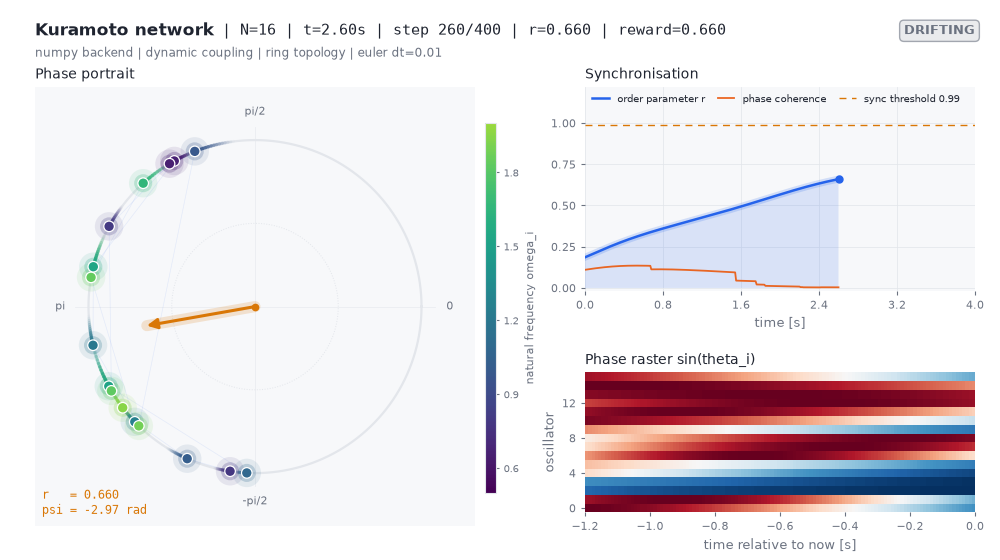
\includegraphics[width=\figwidth]{kuramoto.png}
  \caption{Kuramoto dashboard (16 oscillators on a ring, dynamic coupling,
    light theme). Left: phase portrait with coupling chords, trails and the
    order-parameter vector. Right: order parameter and phase coherence over
    time, and the phase raster $\sin\theta_i$.}
  \label{fig:kuramoto}
\end{figure}

% ---------------------------------------------------------------------------
\section{Registered ids}\label{sec:kuramoto-ids}

\begin{table}[htbp]
  \centering\small
  \caption{Kuramoto ids (all other parameters keep their defaults).}
  \label{tab:kuramoto-ids}
  \begin{tabularx}{\textwidth}{@{}>{\raggedright\arraybackslash}p{0.52\textwidth}X@{}}
    \toprule
    Id & Configuration \\
    \midrule
    \envid{KuramotoOscillator-v0} & NumPy, $N = 10$, dynamic coupling \\
    \envid{KuramotoOscillator-v1} & NumPy, $N = 5$, dynamic coupling \\
    \envid{KuramotoOscillator-Constant-v0} & NumPy, $N = 6$, constant coupling \\
    \envid{KuramotoOscillator-FreqSync-Constant-v0} & NumPy, $N = 6$, constant coupling, frequency reward, $\Omega = 2$ \\
    \envid{KuramotoOscillatorTorch-v0} & PyTorch, $N = 10$, one system \\
    \envid{KuramotoOscillatorTorch-v1} & PyTorch, $N = 8$, 4 systems, CPU \\
    \envid{KuramotoOscillatorTorch-v2} & PyTorch, $N = 10$, RK4, \code{device="auto"} \\
    \envid{KuramotoOscillatorTorch-Constant-v0} & PyTorch, $N = 6$, constant coupling \\
    \envid{KuramotoOscillatorTorch-FreqSync-Constant-v0} & PyTorch, $N = 6$, constant coupling, frequency reward, $\Omega = 2$ \\
    \bottomrule
  \end{tabularx}
\end{table}

% ---------------------------------------------------------------------------
\section{Usage}\label{sec:kuramoto-usage}

The first example drives a network with constant coupling to synchronisation
with a proportional phase-alignment input $a_i = r \sin(\psi - \theta_i)$
computed from the observation:

\begin{pycode}
import numpy as np
import env_lib

env = env_lib.KuramotoOscillatorEnv(
    n_oscillators=12, coupling_mode="constant", coupling_strength=0.5, max_steps=1000
)
obs, info = env.reset(seed=0)
n = env.n_oscillators
while True:
    phases = obs[:n].astype(np.float64)
    z = np.exp(1j * phases).mean()                      # r exp(i psi)
    action = np.abs(z) * np.sin(np.angle(z) - phases)   # phase alignment
    obs, reward, terminated, truncated, info = env.step(action.astype(np.float32))
    if terminated or truncated:
        break
print(info["step_count"], info["order_parameter"])      # synchronised after 51 steps
env.close()
\end{pycode}

The second example runs four systems in parallel on the PyTorch backend, one
coupling level per system:

\begin{pycode}
import numpy as np
import env_lib

env = env_lib.make("KuramotoOscillatorTorch-v1")   # 8 oscillators, 4 systems
core = env.unwrapped
obs, info = env.reset(seed=0)
print(core.get_batch_observations().shape)         # torch.Size([4, 52])

n, act_dim = core.n_oscillators, core.action_space.shape[0]
actions = np.zeros((core.n_agents, act_dim), dtype=np.float32)
actions[:, n:] = np.linspace(1.0, 4.0, core.n_agents)[:, None]
for _ in range(300):
    obs, reward, terminated, truncated, info = env.step(actions)
print(info["order_parameter"])                     # one value per system
print(info["agent_rewards"])                       # per-system rewards incl. bonus
env.close()
\end{pycode}

The example script \code{examples/kuramoto\_demo.py} ramps the coupling
strengths and adds phase alignment, and records the transition from incoherence
to synchronisation:

\begin{shellcode}
python examples/kuramoto_demo.py --save renders/kuramoto.gif
python examples/kuramoto_demo.py --backend torch --n-agents 4 --theme light
python examples/kuramoto_demo.py --mode constant --topology two_clusters --render-mode human
\end{shellcode}

% ---------------------------------------------------------------------------
\section{Reproducibility and performance}\label{sec:kuramoto-perf}

\paragraph{Seeding.} \code{reset(seed=s)} seeds \code{self.np\_random}, from
which the NumPy backend draws the initial state and the phase noise. The
PyTorch backend seeds its own \code{torch.Generator} from
\code{self.np\_random} at every reset; neither backend touches the global
random state. The random topology is built once from \code{topology\_seed}. The
two backends draw from different generators, so the same seed gives different
initial states; to compare them, pass the initial state through
\code{reset(options=...)}.

\paragraph{Performance.} Table~\ref{tab:kuramoto-perf} lists step times
measured with \code{benchmarks/benchmark\_envs.py} on the development machine
(random actions, no rendering). The coupling term is evaluated with two
matrix--vector products instead of $N^2$ sine evaluations. Rendering in
\code{"rgb\_array"} mode takes about 25--35\,ms per frame and dominates the
cost of recorded rollouts; use \code{render\_every} in \code{record\_episode} to
thin out long episodes. Use Euler integration for speed and RK4 when accuracy
at larger \code{dt} matters, and a GPU for large batches.

\begin{table}[htbp]
  \centering\small
  \caption{Step time in milliseconds on the development machine.}
  \label{tab:kuramoto-perf}
  \begin{tabular}{@{}lrr@{}}
    \toprule
    Case & Before 1.0 & Version 1.0 \\
    \midrule
    NumPy, $N = 10$ & 0.17 & 0.04 \\
    NumPy, $N = 50$ & 2.36 & 0.07--0.11 \\
    NumPy, RK4, $N = 50$ & 7.1 & 0.1 \\
    PyTorch (CPU), $N = 50$, 8 systems & 10.3 & 0.3--0.4 \\
    \bottomrule
  \end{tabular}
\end{table}

% ---------------------------------------------------------------------------
\section{Changes in 1.0}\label{sec:kuramoto-changes}

The behaviour of the Kuramoto environments changed in several ways; see
Appendix~\ref{app:migration} for migration advice.

\begin{itemize}
  \item The PyTorch backend had a sign error that made the coupling repulsive
        ($\sin(\theta_i - \theta_j)$ instead of $\sin(\theta_j - \theta_i)$).
        Both backends now implement \eqref{eq:kuramoto} and produce the same
        trajectories; normalisation by $N$ is opt-in for both.
  \item The coupling uses the full matrix; the former NumPy loop skipped entries
        $K_{ij} \le 0$. Default settings are unaffected.
  \item Synchronisation sets \code{terminated} and the step limit sets
        \code{truncated} (previously both were reported as \code{terminated});
        \code{sync\_threshold} and \code{sync\_bonus} are configurable.
  \item Constant mode without a matrix uses
        \code{coupling\_strength}$\,\cdot A$, so the \code{*-Constant-v0} ids
        work (they raised before).
  \item The environments no longer call \code{np.random.seed(42)} or
        \code{torch.manual\_seed(42)}; the random topology uses a local
        generator (\code{topology\_seed}) and is unchanged.
  \item The PyTorch backend accepts \code{device="auto"}, and its phase
        coherence and bonus rules match the NumPy backend.
  \item The dynamics are vectorised (20 times faster at $N = 50$, 65 times with
        RK4) and the renderer was rewritten; the former \code{"rgb\_array"} path
        failed with matplotlib 3.10 and later.
  \item \code{env\_lib.kos\_env.register()} is deprecated; the ids are
        registered when \pkg{env\_lib} is imported.
\end{itemize}

\endgroup

% ---------------------------------------------------------------------------
% Networked communication environments: LineMsg and WirelessComm
% ---------------------------------------------------------------------------
\begingroup
% Line breaking for paragraphs with long, unbreakable identifiers (local to
% this chapter): allow looser lines instead of overfull ones.
\setlength{\emergencystretch}{3em}\tolerance=1000
\chapter{Networked Communication Environments}\label{chap:networked}

This chapter documents two discrete multi-agent benchmarks in which agents on a
network cooperate under local observations:

\begin{itemize}
  \item \textbf{LineMsg} (\code{env\_lib.linemsg\_env.LineMsgEnv}): agents on
        a line relay a message from a source to a sink;
  \item \textbf{WirelessComm}
        (\code{env\_lib.wireless\_comm\_env.WirelessCommEnv}): agents on a grid
        send deadline-constrained packets to shared access points and must avoid
        collisions.
\end{itemize}

Both environments have small discrete state and action spaces, local
observation windows controlled by \code{n\_obs\_neighbors}, per-agent rewards
and a fixed episode length. They are designed for research on decentralised
and networked multi-agent reinforcement learning: exploiting the locality of
interactions (policies and value functions that depend on a $\kappa$-hop
neighbourhood), credit assignment, communication and coordination protocols,
scalability in the number of agents, and robustness to failing agents. The
WirelessComm environment is the Gymnasium joint-action port of an earlier
PettingZoo implementation used in the DSDP project.

% ===========================================================================
\section{LineMsg}\label{sec:linemsg}

% ---------------------------------------------------------------------------
\subsection{Model}\label{sec:linemsg-model}

$N$ agents sit on a line. Agent $N-1$ at the right end is the source, agent 0
at the left end is the sink. Each agent holds a binary state $s_i \in \{0, 1\}$
(1: it holds the message) and chooses a binary action $a_i \in \{0, 1\}$ at
every step. All states are updated synchronously from the previous states:
\begin{align}
  s_0 &\leftarrow s_1, \nonumber\\
  s_i &\leftarrow a_i \wedge \bigl(s_{i+1} \vee [u_i < 0.8]\bigr),
       \qquad 0 < i < N-1,\; u_i \sim \mathcal{U}(0, 1), \label{eq:linemsg}\\
  s_{N-1} &\leftarrow a_{N-1}. \nonumber
\end{align}
An active middle agent ($a_i = 1$) therefore receives the message from its
right neighbour for sure and otherwise obtains one with probability 0.8; an
inactive agent loses its message. The sink copies agent 1 and its own action
has no effect; the source holds the message exactly when it acts. At reset all
agents hold the message ($s_i = 1$).

\paragraph{Reward.} Agent $i$ receives
\begin{equation}
  r_i = w_i\, s_i, \qquad w_0 = 1.0, \quad w_i = 0.1 \;\; (i > 0),
\end{equation}
evaluated on the new states, and the team reward is $R = \sum_i r_i$. The
maximum per step is $1 + 0.1(N - 1)$, which the ``always relay'' policy
($a_i = 1$ for all $i$) attains at every step.

\paragraph{Episode end.} \code{terminated} is always \code{False};
\code{truncated} becomes \code{True} after \code{max\_iter} steps.

% ---------------------------------------------------------------------------
\subsection{Spaces}\label{sec:linemsg-spaces}

\paragraph{Action.} The joint action can be given in two formats, both of
which \code{step()} always accepts:
\begin{itemize}
  \item an integer in \code{Discrete(2**N)} whose bit $i$ is the action of
        agent $i$ (the declared space for \code{action\_space\_type="discrete"},
        the default; only possible for $N \le 62$);
  \item an array of $N$ values in $\{0, 1\}$ (integer or boolean), the
        declared space \code{MultiBinary(N)} for
        \code{action\_space\_type="multibinary"}, which has no limit on $N$.
\end{itemize}
Out-of-range integers, arrays of the wrong shape and values other than 0 and 1
raise \code{ValueError}.

\paragraph{Observation.} \code{Box(0, 3, (N, 2k+1), float32)} with
$k$ = \code{n\_obs\_neighbors}. The state vector is padded with $k$ boundary
cells on each side, and row $i$ is the window of the $2k + 1$ cells centred on
agent $i$:

\begin{table}[htbp]
  \centering\small
  \caption{LineMsg observation (row $i$).}
  \label{tab:linemsg-obs}
  \begin{tabularx}{\textwidth}{@{}l>{\raggedright\arraybackslash}X@{}}
    \toprule
    Column & Content \\
    \midrule
    \code{0 : k} & states of agents $i-k, \dots, i-1$ (left neighbours, towards the sink) \\
    \code{k} & own state $s_i$ \\
    \code{k+1 : 2k+1} & states of agents $i+1, \dots, i+k$ (right neighbours, towards the source) \\
    \midrule
    Values & 0: no message, 1: message, 2: boundary cell beyond the end of the line \\
    \bottomrule
  \end{tabularx}
\end{table}

% ---------------------------------------------------------------------------
\subsection{Parameters and info}\label{sec:linemsg-params}

\begin{table}[htbp]
  \centering\small
  \caption{Constructor parameters of \code{LineMsgEnv}.}
  \label{tab:linemsg-params}
  \begin{tabularx}{\textwidth}{@{}>{\raggedright\arraybackslash}p{0.25\textwidth}>{\raggedright\arraybackslash}p{0.14\textwidth}>{\raggedright\arraybackslash}X@{}}
    \toprule
    Parameter & Default & Description \\
    \midrule
    \code{num\_agents} & \code{10} & Number of agents $N$ ($\ge 2$: a sink and a source, plus any number of relays). \\
    \code{n\_obs\_neighbors} & \code{1} & Observation radius $k$; $0$ is treated as $1$ with a warning. \\
    \code{max\_iter} & \code{50} & Episode length; reaching it sets \code{truncated}. \\
    \code{render\_mode} & \code{None} & \code{None}, \code{"human"}, \code{"rgb\_array"} or \code{"ansi"}. \\
    \code{action\_space\_type} & \code{"discrete"} & Declared action space: \code{"discrete"} (\code{Discrete(2**N)}, $N \le 62$) or \code{"multibinary"} (\code{MultiBinary(N)}). \\
    \bottomrule
  \end{tabularx}
\end{table}

The info dictionary of \code{reset()} and \code{step()} contains a single key,
\code{"agent\_rewards"}: the \code{float64} per-agent rewards $r_i$ (zeros at
reset). The attribute \code{state} holds the padded state vector (agent $i$ is
\code{state[k + i]}), \code{actions} the last joint action with the same padding
(2 before the first step), and \code{num\_moves} the number of steps taken.
\code{step()} before \code{reset()} raises \code{env\_lib.ResetNeededError}.

% ---------------------------------------------------------------------------
\subsection{Rendering}\label{sec:linemsg-render}

The dashboard (Figure~\ref{fig:linemsg}) shows the line of agents at the top,
coloured by state, with a halo under agents that act and arrows on the active
links, which point in the direction of message flow towards the sink. Below it
a space-time raster (one row per step, one column per agent) makes message
fronts visible, and the right panel traces the team reward with its maximum.
The header reports the step, the last reward, the episode return and the number
of agents holding the message. \code{render\_mode="ansi"} returns a text line
with the action and state of every agent.

\begin{figure}[htbp]
  \centering
  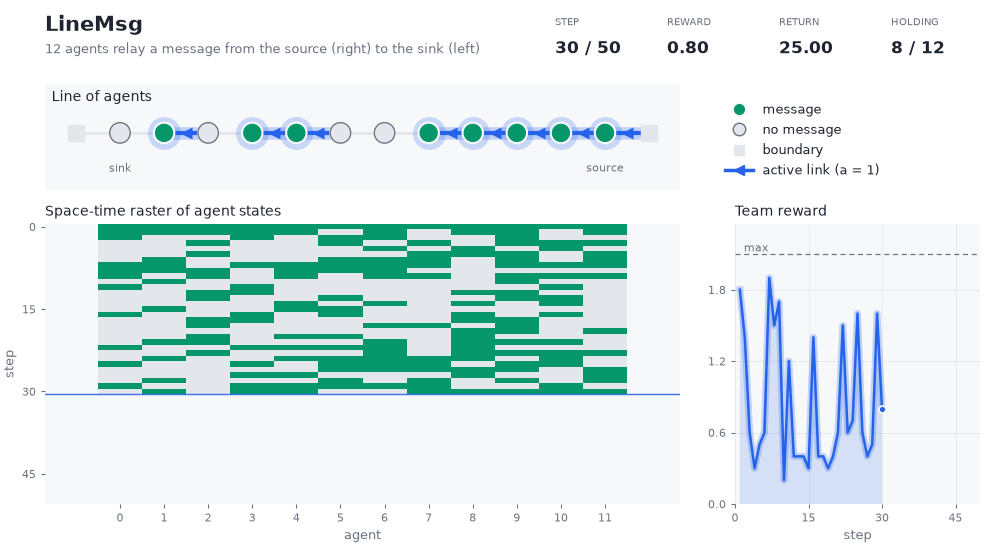
\includegraphics[width=\figwidth]{linemsg.png}
  \caption{LineMsg dashboard (12 agents, step 30 of 50).
    Top: agent states and active links. Bottom left: space-time raster of the
    agent states. Bottom right: team reward per step.}
  \label{fig:linemsg}
\end{figure}

% ---------------------------------------------------------------------------
\subsection{Usage}\label{sec:linemsg-usage}

\begin{pycode}
import numpy as np
from env_lib.linemsg_env import LineMsgEnv

env = LineMsgEnv(num_agents=10, action_space_type="multibinary")
obs, info = env.reset(seed=0)                 # obs: (10, 3) float32
rng = np.random.default_rng(0)
episode_return = 0.0
while True:
    action = (rng.random(env.num_agents) < 0.9).astype(np.int64)  # duty cycle
    obs, reward, terminated, truncated, info = env.step(action)
    episode_return += reward
    if terminated or truncated:
        break
print(episode_return, info["agent_rewards"])

env.reset(seed=1)
env.step(0b1111111110)          # integer action: all agents but the sink act
\end{pycode}

The example script compares a random policy, duty-cycled relays and the
always-relay policy and can record an episode:

\begin{shellcode}
python examples/environments/linemsg_demo.py --policy relay --save renders/linemsg.gif
python examples/environments/linemsg_demo.py --num-agents 30 --episodes 50
python examples/environments/linemsg_demo.py --render-mode ansi
\end{shellcode}

Over 20 episodes with $N = 10$ and \code{max\_iter=50} the mean returns are
44.1 for uniformly random actions, 85.2 for duty-cycled relays that act with
probability 0.9, and 95.0 for the always-relay policy (the maximum).

% ===========================================================================
\section{WirelessComm}\label{sec:wireless}

% ---------------------------------------------------------------------------
\subsection{Model}\label{sec:wireless-model}

$G_x \times G_y$ agents sit on a grid (\code{grid\_x} rows, \code{grid\_y}
columns); agent $(i, j)$ has index $i G_y + j$. Access points sit at the
$(G_x - 1)(G_y - 1)$ interior corners of the grid: access point $(a, b)$ lies
between agents $(a, b)$, $(a+1, b)$, $(a, b+1)$ and $(a+1, b+1)$. Every agent
holds a packet queue with $D$ = \code{ddl} deadline slots; slot 0 holds the
packet with the earliest deadline. Each agent chooses one of five actions per
step (Table~\ref{tab:wireless-actions}).

\begin{table}[htbp]
  \centering\small
  \caption{WirelessComm actions of agent $(i, j)$. A direction without an
    access point (at the border of the grid) is a failed attempt.}
  \label{tab:wireless-actions}
  \begin{tabular}{@{}cll@{}}
    \toprule
    Action & Meaning & Access point \\
    \midrule
    0 & stay idle & none \\
    1 & transmit up-left & $(i-1, j-1)$ \\
    2 & transmit down-left & $(i, j-1)$ \\
    3 & transmit up-right & $(i-1, j)$ \\
    4 & transmit down-right & $(i, j)$ \\
    \bottomrule
  \end{tabular}
\end{table}

\paragraph{Transition.} Let $\ell_m$ be the load of access point $m$, the
number of agents that transmit to it in the step; every transmitting agent
counts, whether or not it holds a packet. The transmission of agent $k$ is
\emph{eligible} when the agent transmits, holds at least one packet, its access
point exists and that access point has load exactly $\ell_m = 1$. Each eligible
transmission succeeds with probability $q$; one uniform draw is made per
eligible agent, in agent order. A success removes the agent's earliest-deadline
packet and earns reward 1. Afterwards every queue shifts one slot towards the
deadline (packets in slot 0 expire and are lost), and a new packet arrives in
the last slot with probability $p$. At reset every queue slot is occupied
independently with probability $1/2$.

\paragraph{Reward and outcomes.} The per-agent reward is 1 for a delivered
packet and 0 otherwise; the team reward is the number of packets delivered in
the step. The outcome of every agent is reported in \code{info["outcomes"]}
(Table~\ref{tab:wireless-info}): idle (0), success (1), collision (2: the
access point exists and has load $\ge 2$) or lost (3: any other failed attempt,
that is no packet, no access point or a channel loss).

\paragraph{Episode end.} \code{terminated} is always \code{False};
\code{truncated} becomes \code{True} after \code{max\_iter} steps.

% ---------------------------------------------------------------------------
\subsection{Spaces}\label{sec:wireless-spaces}

\paragraph{Action.} \code{MultiDiscrete([5] * n)} with $n = G_x G_y$. An action
of shape \code{(n,)} or \code{(grid\_x, grid\_y)} is accepted; other shapes and
values outside $0, \dots, 4$ raise \code{ValueError}.

\paragraph{Observation.} \code{Box(0, 2, (n, D w\^{}2), float32)} with
$w = 2k + 1$ and $k$ = \code{n\_obs\_neighbors}. The queues form a
$(D, G_x, G_y)$ array that is padded with $k$ cells of value 2 on every side of
the grid. Row $m$ of the observation is the $(D, w, w)$ window centred on agent
$m$, flattened in C order (slot, then row, then column). Values are 0 (empty
slot), 1 (packet) and 2 (outside the grid). The agent's own slot $d$ is column
$d w^2 + k w + k$. The default configuration ($D = 2$, $k = 1$) has 18 columns.

% ---------------------------------------------------------------------------
\subsection{Parameters and info}\label{sec:wireless-params}

\begin{table}[htbp]
  \centering\small
  \caption{Constructor parameters of \code{WirelessCommEnv}.}
  \label{tab:wireless-params}
  \begin{tabularx}{\textwidth}{@{}>{\raggedright\arraybackslash}p{0.39\textwidth}>{\raggedright\arraybackslash}p{0.1\textwidth}>{\raggedright\arraybackslash}X@{}}
    \toprule
    Parameter & Default & Description \\
    \midrule
    \code{grid\_x}, \code{grid\_y} & \code{6}, \code{6} & Number of agent rows and columns (each $\ge 2$, so that at least one access point exists). \\
    \code{ddl} & \code{2} & Deadline horizon $D$: queue slots per agent ($\ge 1$). \\
    \code{packet\_arrival\_probability} & \code{0.8} & Arrival probability $p$ of a new packet per agent and step. \\
    \code{success\_transmission\_probability} & \code{0.8} & Success probability $q$ of an eligible transmission. \\
    \code{n\_obs\_neighbors} & \code{1} & Observation radius $k$ (Chebyshev distance, $\ge 0$). \\
    \code{max\_iter} & \code{50} & Episode length; reaching it sets \code{truncated}. \\
    \code{render\_mode} & \code{None} & \code{None}, \code{"human"}, \code{"rgb\_array"} or \code{"ansi"}. \\
    \bottomrule
  \end{tabularx}
\end{table}

\begin{table}[htbp]
  \centering\small
  \caption{WirelessComm info dictionary (the same keys, all zero, at reset).}
  \label{tab:wireless-info}
  \begin{tabularx}{\textwidth}{@{}l>{\raggedright\arraybackslash}X@{}}
    \toprule
    Key & Content \\
    \midrule
    \code{agent\_rewards} & \code{float64} array \code{(n,)}: 1 for a delivered packet, else 0 \\
    \code{outcomes} & \code{int8} array \code{(n,)}: 0 idle, 1 success, 2 collision, 3 lost
      (constants \code{OUTCOME\_IDLE}, \code{OUTCOME\_SUCCESS}, \code{OUTCOME\_COLLISION},
      \code{OUTCOME\_LOST} and \code{OUTCOME\_LABELS} in \code{env\_lib.wireless\_comm\_env.wireless\_comm\_env}) \\
    \code{ap\_load} & \code{int64} array \code{(grid\_x - 1, grid\_y - 1)}: number of agents that transmitted to each access point \\
    \bottomrule
  \end{tabularx}
\end{table}

The environment also exposes \code{last\_outcomes} and \code{last\_ap\_load}
(the values of the last step), \code{access\_point\_mapping(i, j, action)},
which returns the access point $(a, b)$ reached by agent $(i, j)$ or
\code{(None, None)}, and \code{check\_transmission\_fail(a, b, load)}.
\code{step()} before \code{reset()} raises \code{env\_lib.ResetNeededError}.

% ---------------------------------------------------------------------------
\subsection{Rendering}\label{sec:wireless-render}

The dashboard (Figure~\ref{fig:wireless}) draws the agent grid on the left.
Every agent is a circle coloured by the outcome of its last action, with a
small queue bar below it (one cell per deadline slot; the left cell expires
first). Access points are squares at the interior corners, coloured by their
load (idle, one transmitter, collision), and a line joins every transmitting
agent to the access point it chose, coloured by the outcome; the line of an attempt
towards a missing access point ends outside the grid. The right panels show the packets
delivered per step with a rolling mean and the rolling collision count, and the
cumulative return. \code{render\_mode="ansi"} returns the action and queue of
every agent as text.

\begin{figure}[htbp]
  \centering
  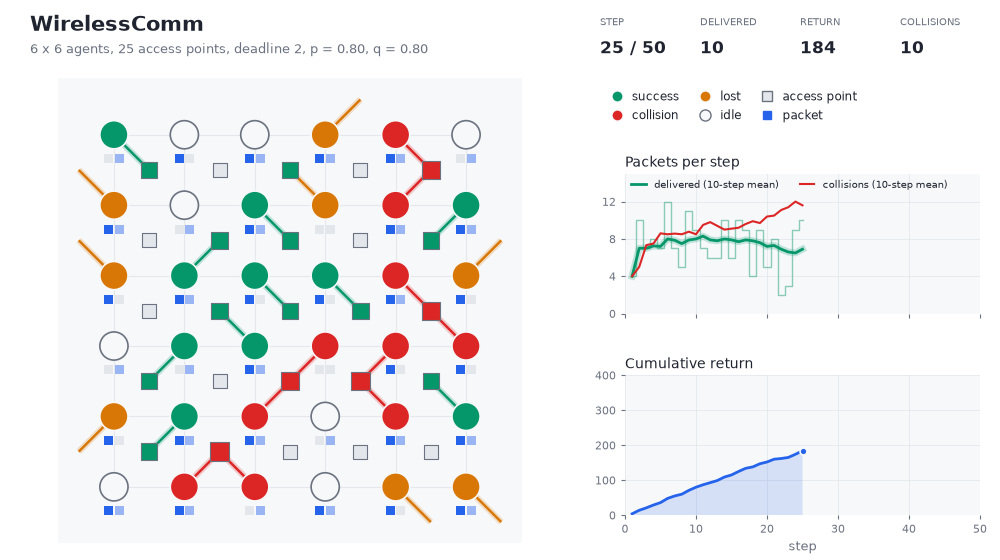
\includegraphics[width=\figwidth]{wireless.png}
  \caption{WirelessComm dashboard ($6 \times 6$ agents, 25 access points,
    step 25 of 50). Left: agents coloured by outcome with their packet queues,
    access points coloured by load and transmission links. Right: packets
    delivered and collisions per step (10-step means) and the cumulative
    return.}
  \label{fig:wireless}
\end{figure}

% ---------------------------------------------------------------------------
\subsection{Usage}\label{sec:wireless-usage}

The following policy is a collision-free rotating schedule: at step $t$ every
agent that holds a packet uses the same direction $(4, 1, 2, 3)[t \bmod 4]$ if
an access point exists in that direction. A common direction maps agents to
access points one-to-one, so no collisions occur.

\begin{pycode}
import numpy as np
from env_lib.wireless_comm_env import WirelessCommEnv

env = WirelessCommEnv(grid_x=6, grid_y=6)
obs, info = env.reset(seed=0)                     # obs: (36, 18) float32
k, w = env.n_obs_nghbr, env.window
own = [d * w * w + k * w + k for d in range(env.ddl)]  # own queue columns
directions = (4, 1, 2, 3)
cells = [(i, j) for i in range(env.grid_x) for j in range(env.grid_y)]
reachable = {d: np.array([env.access_point_mapping(i, j, d)[0] is not None
                          for i, j in cells])
             for d in directions}
episode_return = 0.0
for t in range(env.max_iter):
    d = directions[t % 4]
    has_packet = obs[:, own].max(axis=1) > 0.5
    action = np.where(has_packet & reachable[d], d, 0)
    obs, reward, terminated, truncated, info = env.step(action)
    episode_return += reward
print(episode_return, np.bincount(info["outcomes"], minlength=4))
\end{pycode}

The example script compares uniformly random actions, $p$-persistent slotted
ALOHA and the rotating schedule:

\begin{shellcode}
python examples/environments/wireless_comm_demo.py --policy schedule \
    --save renders/wireless.gif
python examples/environments/wireless_comm_demo.py --grid 8 8 --tau 0.5 --episodes 50
\end{shellcode}

Over 20 episodes on the $6 \times 6$ grid the mean returns are 385 for random
actions, 398 for ALOHA with transmit probability 0.6 and 910 for the rotating
schedule, which causes no collisions.

% ===========================================================================
\section{Registered ids}\label{sec:networked-ids}

\begin{table}[htbp]
  \centering\small
  \caption{Registered ids of the networked environments.}
  \label{tab:networked-ids}
  \begin{tabular}{@{}lll@{}}
    \toprule
    Id & Class & Configuration \\
    \midrule
    \envid{LineMsg-v0} & \code{LineMsgEnv} & defaults (10 agents) \\
    \envid{WirelessComm-v0} & \code{WirelessCommEnv} & defaults ($6 \times 6$ grid, 36 agents) \\
    \envid{WirelessComm-v1} & \code{WirelessCommEnv} & \code{grid\_x=4}, \code{grid\_y=4} (16 agents) \\
    \bottomrule
  \end{tabular}
\end{table}

% ===========================================================================
\section{Reproducibility and performance}\label{sec:networked-perf}

Both environments draw all randomness (relay successes in LineMsg; initial
queues, transmission successes and packet arrivals in WirelessComm) from
\code{self.np\_random}, seeded by \code{reset(seed=...)}. Seeded trajectories
are bit-identical to those of the implementation before version 1.0, so
earlier results can be reproduced exactly.

Measured on the development machine without rendering, a LineMsg step with 10
agents takes 0.013\,ms (0.019\,ms before 1.0), and a WirelessComm step takes
0.05\,ms on the $6 \times 6$ grid (0.154\,ms before) and 0.046\,ms on a
$12 \times 12$ grid (0.56\,ms before). Rendering a dashboard frame in
\code{"rgb\_array"} mode takes about 15\,ms for either environment; the history
needed by the dashboards is only recorded in the \code{"human"} and
\code{"rgb\_array"} modes.

% ===========================================================================
\section{Changes in 1.0}\label{sec:networked-changes}

The seeded dynamics of both environments are unchanged. Interface changes are
summarised below; see Appendix~\ref{app:migration} for migration advice.

\paragraph{LineMsg.}
\begin{itemize}
  \item Action decoding and observations are vectorised.
  \item The joint action may be an integer or an array of $N$ bits. The new
        option \code{action\_space\_type="multibinary"} declares a
        \code{MultiBinary(N)} space and supports more than 62 agents.
  \item \code{step()} before \code{reset()} raises instead of resetting
        implicitly.
  \item The former text output is \code{render\_mode="ansi"}; \code{"human"}
        and \code{"rgb\_array"} show the new dashboard.
\end{itemize}

\paragraph{WirelessComm.}
\begin{itemize}
  \item \code{step()} is fully vectorised (up to 37 times faster on large grids).
  \item Fixed: the stored actions were never updated, so rendering showed no
        actions. Per-agent outcomes and access-point loads are reported in
        \code{info}.
  \item Arguments and actions are validated; \code{"ansi"} text mode and a new
        dashboard were added.
  \item \code{env\_lib.wireless\_comm\_env.register()} is deprecated; the ids
        are registered when \pkg{env\_lib} is imported.
\end{itemize}

\endgroup

% ---------------------------------------------------------------------------
% Pistonball environment
% ---------------------------------------------------------------------------
\begingroup
% Line breaking for paragraphs with long, unbreakable identifiers (local to
% this chapter): allow looser lines instead of overfull ones.
\setlength{\emergencystretch}{3em}\tolerance=1000
\chapter{Pistonball}\label{chap:pistonball}

Pistonball is a cooperative physics game. A row of pistons forms the floor of a
walled arena and a ball is dropped near the right wall; every piston is an
agent that moves up or down, and together the pistons must roll the ball to
the left wall. Each piston observes the ball only when it is close to it, and
the reward of a piston depends on the ball's progress while it observes the
ball. The environment is used to study cooperation under local observability,
credit assignment with local rewards, scalability in the number of agents and
the effect of the observation radius $\kappa$ on learning. The physics is
simulated with \pkg{pymunk}; \pkg{pygame} is only needed for rendering and
keyboard control (extra \code{pistonball}).

The class is \code{env\_lib.pistonball\_env.PistonballEnv}; the package also
exports \code{ManualPolicy}, \code{PistonballRenderer} and
\code{PistonballLayout}.

% ---------------------------------------------------------------------------
\section{Arena and physics}\label{sec:pistonball-physics}

All coordinates are pygame screen pixels with $y$ growing downwards. With $n$
pistons the screen is $W = 160 + 40n$ pixels wide and 560 pixels high; the
walls are 80 pixels from each screen edge, so the arena spans
$x \in [80, W - 80]$ and $y \in [80, 480]$. The left wall is the goal.

\begin{itemize}
  \item \textbf{Pistons.} Piston $i$ is 40 pixels wide with its left edge at
        $x = 80 + 40i$. Its height $y_i$ (the $y$ coordinate of the piston
        head) moves by 4 pixels per unit action and is limited to
        $y_i \in [387, 451]$, a travel of 64 pixels around the middle position
        419. At reset every piston starts at $451 - d_i$ with $d_i$ drawn
        uniformly from $\{0, 4, \dots, 28\}$.
  \item \textbf{Ball.} A disc of radius 40 pixels with mass
        \code{ball\_mass}, friction \code{ball\_friction} and elasticity
        \code{ball\_elasticity}. It starts at
        $x = W - 150 + \delta_x$, $y = 370 + \delta_y$, where
        $\delta_x \in \{-30, \dots, 30\}$ and $\delta_y \in \{-15, \dots, 15\}$
        are uniform integers when \code{random\_drop=True} and zero otherwise,
        with an angular velocity drawn uniformly from $[-6\pi, 6\pi]$\,rad/s
        when \code{random\_rotate=True}.
  \item \textbf{Simulation.} Gravity is 750\,px/s$^2$ downwards, walls and
        pistons have friction 0.64, and one environment step is one physics
        step of $\Delta t = 1/20$\,s. The pistons are kinematic bodies that are
        moved to their new height before the physics step; the ball speed is
        capped at 1000\,px/s and its position is kept inside the screen.
\end{itemize}

% ---------------------------------------------------------------------------
\section{Spaces}\label{sec:pistonball-spaces}

\paragraph{Action.} One value per piston, stacked in an array of shape
\code{(n,)}:
\begin{itemize}
  \item continuous (\code{continuous=True}, default):
        \code{Box(-1, 1, (n,), float32)}; the value is clipped to $[-1, 1]$ and
        moves the piston by $4 a_i$ pixels, where $+1$ moves it up;
  \item discrete (\code{continuous=False}): \code{MultiDiscrete([3] * n)} with
        0 = down, 1 = stay and 2 = up (4 pixels).
\end{itemize}
Actions of the wrong shape, continuous actions with NaN or infinite values, and
discrete values outside $\{0, 1, 2\}$ raise \code{ValueError}.

\paragraph{Observation.} \code{float32} array of shape \code{(n, 7)} in an
unbounded \code{Box}. Row $i$ is the observation of piston $i$
(Table~\ref{tab:pistonball-obs}). The piston under the ball has index
\begin{equation}
  p(x) = \operatorname{clip}\bigl(\lfloor (x - 85)/40 \rfloor,\; 0,\; n - 1\bigr),
\end{equation}
and piston $i$ observes the ball when $|i - p(x)| \le \kappa$, where $x$ is the
ball centre and $\kappa$ = \code{kappa}. Columns 2--6 are zero for pistons that
do not observe the ball. The method \code{observable\_mask()} returns the
boolean mask of the observing pistons; its optional argument \code{ball\_x}
evaluates the mask for another ball position.

\begin{table}[htbp]
  \centering\small
  \caption{Pistonball observation (row $i$). $(x, y)$ is the ball centre,
    $(v_x, v_y)$ its velocity in px/s and $\dot\phi$ its angular velocity.}
  \label{tab:pistonball-obs}
  \begin{tabularx}{\textwidth}{@{}cl>{\raggedright\arraybackslash}X@{}}
    \toprule
    Column & Value & Meaning \\
    \midrule
    0 & $(y_i - 419)/32$ & piston height in $[-1, 1]$; $+1$ is the lowest position \\
    1 & $(5 + 40i)/(40n)$ & piston position along the arena in $[0, 1]$ \\
    2 & $(x - 80)/(40n)$ & ball $x$ position (observers only) \\
    3 & $(y - 80)/400$ & ball $y$ position (observers only) \\
    4 & $v_x / 15$ & ball $x$ velocity (observers only) \\
    5 & $v_y / 8$ & ball $y$ velocity (observers only) \\
    6 & $\dot\phi / 8$ & ball angular velocity (observers only) \\
    \bottomrule
  \end{tabularx}
\end{table}

% ---------------------------------------------------------------------------
\section{Reward and episode end}\label{sec:pistonball-reward}

Let $b_t = \lfloor x_t - 40 \rfloor$ be the $x$ coordinate of the ball's left
edge after step $t$ and $\Delta b = b_{t-1} - b_t$ its leftward displacement.
The ball term rewards leftward progress at half rate and penalises rightward
motion in full:
\begin{equation}
  g_t =
  \begin{cases}
    0.5\,\Delta b, & \Delta b > 0,\\
    \Delta b, & \text{otherwise.}
  \end{cases}
\end{equation}
The local reward of piston $i$ is
\begin{equation}
  \begin{split}
  r_i = \tau
      &+ g_t\, \mathbf{1}\bigl[i \in O(b_{t-1}) \cup O(b_t)\bigr]
       + \rho_T\, \mathbf{1}\bigl[\text{goal},\; i \in O(x_t)\bigr]
       + \rho_L\, \mathbf{1}\bigl[\text{goal},\; i = 0\bigr] \\
      &+ \mu\, \frac{|\Delta y_i|}{4}\, \mathbf{1}\bigl[|\Delta y_i| > \epsilon_\mu\bigr],
  \end{split}
  \label{eq:pistonball-reward}
\end{equation}
where $O(z) = \{ i : |i - p(z)| \le \kappa \}$ is the set of pistons within
$\kappa$ hops of the piston under position $z$ (the ball term uses the left-edge
positions $b$, the goal bonus the ball centre $x_t$), $\tau$ =
\code{time\_penalty}, $\rho_T$ = \code{termination\_reward}, $\rho_L$ =
\code{leftmost\_piston\_reward}, $\mu$ = \code{movement\_penalty},
$\epsilon_\mu$ = \code{movement\_penalty\_threshold} and $\Delta y_i$ the
movement of piston $i$ in pixels. The team reward returned by \code{step()} is
$R = \sum_i r_i$.

\paragraph{Goal and episode end.} With \code{terminated\_condition=True}
(default) the goal is reached when the ball's left edge will reach the left wall
within one step, $x_t - 40 + v_x \Delta t \le 80.5$; the episode then
terminates. \code{truncated} becomes \code{True} after \code{max\_cycles}
steps. For example, with \code{leftmost\_piston\_reward=1.0} and the default
termination reward, piston 0 receives $0.5 + 1.0 = 1.5$ on reaching the goal,
the other pistons that observe the ball receive 0.5, and the remaining pistons
receive no bonus.

% ---------------------------------------------------------------------------
\section{Parameters}\label{sec:pistonball-params}

\begingroup\small
\begin{longtable}{@{}>{\raggedright\arraybackslash}p{0.33\textwidth}>{\raggedright\arraybackslash}p{0.1\textwidth}>{\raggedright\arraybackslash}p{0.51\textwidth}@{}}
  \caption{Constructor parameters of \code{PistonballEnv}.}\label{tab:pistonball-params}\\
  \toprule
  Parameter & Default & Description \\
  \midrule
  \endfirsthead
  \toprule
  Parameter & Default & Description \\
  \midrule
  \endhead
  \bottomrule
  \endfoot
  \code{n\_pistons} & \code{20} & Number of pistons (agents), $\ge 1$. \\
  \code{time\_penalty} & \code{-0.1} & Reward $\tau$ added to every piston at every step. \\
  \code{continuous} & \code{True} & Continuous actions in $[-1, 1]$; \code{False} for \code{MultiDiscrete([3] * n)}. \\
  \code{random\_drop} & \code{True} & Randomise the initial ball position ($\pm 30$\,px horizontally, $\pm 15$\,px vertically). \\
  \code{random\_rotate} & \code{True} & Random initial angular velocity in $[-6\pi, 6\pi]$\,rad/s. \\
  \code{ball\_mass} & \code{0.75} & Ball mass ($> 0$). \\
  \code{ball\_friction} & \code{0.3} & Ball friction ($\ge 0$). \\
  \code{ball\_elasticity} & \code{1.5} & Ball elasticity ($\ge 0$). \\
  \code{max\_cycles} & \code{125} & Episode length; reaching it sets \code{truncated}. \\
  \code{render\_mode} & \code{None} & \code{None}, \code{"human"} (pygame window) or \code{"rgb\_array"}. \\
  \code{movement\_penalty} & \code{0.0} & Reward $\mu$ per 4 pixels of piston movement, typically negative; 0 disables it. \\
  \code{movement\_penalty\_threshold} & \code{0.01} & Movements of at most this many pixels are not penalised. \\
  \code{kappa} & \code{1} & Observation radius $\kappa$ in pistons ($\ge 0$). \\
  \code{terminated\_condition} & \code{True} & End the episode when the ball reaches the left wall. \\
  \code{leftmost\_piston\_reward} & \code{0.0} & Bonus $\rho_L$ for piston 0 when the goal is reached. \\
  \code{termination\_reward} & \code{0.5} & Bonus $\rho_T$ for every piston that observes the ball when the goal is reached. \\
\end{longtable}
\endgroup

\paragraph{Physics presets.} The ball parameters change the character of the
task considerably. A heavy, damped ball (\code{ball\_mass=2.0},
\code{ball\_friction=0.8}, \code{ball\_elasticity=0.5}) rolls slowly and rewards
coordinated ramps; a light, bouncy ball (\code{ball\_mass=0.5},
\code{ball\_friction=0.1}, \code{ball\_elasticity=2.0}) is harder to control.

\paragraph{Info dictionary.} \code{step()} returns \code{"local\_rewards"} and
\code{"agent\_rewards"} (both the \code{float64} local rewards $r_i$, shape
\code{(n,)}) and \code{"total\_reward"} (their sum, equal to the returned
reward). The info dictionary of \code{reset()} is empty. \code{step()} before
\code{reset()} raises \code{RuntimeError}.

% ---------------------------------------------------------------------------
\section{Keyboard control}\label{sec:pistonball-manual}

\code{ManualPolicy(env, agent\_id=0, show\_obs=False)} lets a person control one
piston at a time in a window. Create the environment with
\code{render\_mode="human"} so that the pygame window exists and receives the
key presses, and call the policy once per step: \code{W} or \code{Up} raises
the selected piston, \code{S} or \code{Down} lowers it (hold the key to keep
moving), \code{A}/\code{Left} and \code{D}/\code{Right} select the previous or
next piston, \code{Backspace} resets the environment, and \code{Esc} or closing
the window sets \code{policy.running} to \code{False}. All other pistons stay
in place.

\begin{pycode}
from env_lib.pistonball_env import ManualPolicy, PistonballEnv

env = PistonballEnv(n_pistons=8, render_mode="human")
policy = ManualPolicy(env)
obs, info = env.reset(seed=0)
while policy.running:
    obs, reward, terminated, truncated, info = env.step(policy(obs))
    if terminated or truncated:
        obs, info = env.reset()
env.close()
\end{pycode}

% ---------------------------------------------------------------------------
\section{Rendering}\label{sec:pistonball-render}

The renderer draws with pygame and needs no image assets
(Figure~\ref{fig:pistonball}). It shows a gradient background with shaded walls
and a highlighted goal strip on the left wall, the pistons as rounded
rectangles (pistons that observe the ball in the accent colour with a glow),
the ball with shading, a rotation marker and a fading motion trail, a
heads-up display with the step counter, episode return, ball $x$ velocity and
number of observing pistons, and a progress bar with the ball's distance to the
goal. Frames have the screen size, $(160 + 40n) \times 560$ pixels. The
\code{"rgb\_array"} mode never initialises the display and works on headless
machines; \code{"human"} mode opens a window capped at 20 frames per second.
Colours follow the active theme (Section~\ref{sec:envlib-rendering}).

\begin{figure}[htbp]
  \centering
  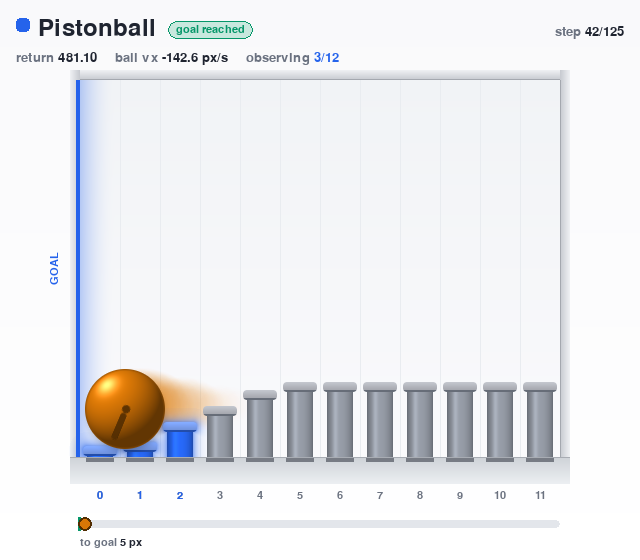
\includegraphics[width=0.62\textwidth]{pistonball.png}
  \caption{Pistonball with 12 pistons (light theme) at the moment the ball
    reaches the goal. The three pistons that observe the ball ($\kappa = 1$)
    are highlighted; the ramp formed by the pistons rolls the ball to the
    left wall.}
  \label{fig:pistonball}
\end{figure}

% ---------------------------------------------------------------------------
\section{Registered id}\label{sec:pistonball-ids}

\envid{Pistonball-v0} creates \code{PistonballEnv} with its defaults (20
pistons, continuous actions, $\kappa = 1$). Creating it requires \pkg{pymunk};
rendering also requires \pkg{pygame}.

% ---------------------------------------------------------------------------
\section{Usage}\label{sec:pistonball-usage}

The following heuristic reads the ball position from the observing pistons and
shapes the pistons into a ramp that falls towards the left: pistons right of
the ball move up, pistons left of it move down.

\begin{pycode}
import numpy as np
from env_lib.pistonball_env import PistonballEnv

env = PistonballEnv(n_pistons=12, kappa=1)
obs, info = env.reset(seed=0)                     # obs: (12, 7) float32
episode_return = 0.0
while True:
    action = np.zeros(env.n_pistons, dtype=np.float32)
    observers = np.any(obs[:, 2:] != 0.0, axis=1)
    if observers.any():
        ball_x = obs[observers, 2].mean()          # (x - 80) / (40 n)
        offset = (obs[:, 1] - ball_x) * env.n_pistons  # in piston widths
        action = np.clip(2.0 * offset, -1.0, 1.0).astype(np.float32)
    obs, reward, terminated, truncated, info = env.step(action)
    episode_return += reward
    if terminated or truncated:
        break
print(env.frames, terminated, episode_return)     # goal after 99 steps
env.close()
\end{pycode}

The example script evaluates a similar heuristic against random actions,
records episodes and offers keyboard control:

\begin{shellcode}
python examples/pistonball_demo.py --save renders/pistonball.gif
python examples/pistonball_demo.py --discrete --kappa 2 --movement-penalty -0.05
python examples/pistonball_demo.py --manual --n-pistons 8
\end{shellcode}

Over 20 episodes with the default configuration the heuristic of the script
reaches a mean return of $857.1 \pm 254.3$ and brings the ball to the goal in
95\,\% of the episodes, whereas random actions obtain $-290.5$ and never reach
the goal.

% ---------------------------------------------------------------------------
\section{Reproducibility and performance}\label{sec:pistonball-perf}

\code{reset(seed=...)} seeds \code{self.np\_random}, from which the initial
piston heights, the ball position and its angular velocity are drawn; the
physics itself is deterministic. The random draws are made in the same order as
before version 1.0, so seeded episodes start from the same states as in earlier
versions.

Measured on the development machine with 20 pistons, a step without rendering
takes 0.06\,ms (1.11\,ms before 1.0, when the screen was drawn at every step).
Rendering an \code{"rgb\_array"} frame takes about 3\,ms.

% ---------------------------------------------------------------------------
\section{Changes in 1.0}\label{sec:pistonball-changes}

See Appendix~\ref{app:migration} for migration advice.

\begin{itemize}
  \item Nothing is drawn unless rendering is requested; pygame is initialised
        lazily. Together with vectorised observations and rewards this makes
        steps 16 to 30 times faster.
  \item In discrete mode the declared action space is
        \code{MultiDiscrete([3] * n)}, one entry per piston. The per-piston
        action arrays accepted by \code{step()} are unchanged; the former
        single-integer \code{Discrete(3**n)} declaration was removed.
  \item Actions are validated (shape, range, NaN), and \code{step()} before
        \code{reset()} raises.
  \item New vector renderer (shaded pistons, highlighted $\kappa$-hop
        observers, ball trail, heads-up display, progress bar); the PNG sprites
        were removed. The former drawing methods (\code{draw()},
        \code{draw\_background()}, \code{draw\_pistons()},
        \code{enable\_render()}) are deprecated no-ops.
  \item Compatible with pymunk 6 and 7.
\end{itemize}

\endgroup

% ---------------------------------------------------------------------------
% Consensus and formation control environment
% ---------------------------------------------------------------------------
\begingroup
% Line breaking for paragraphs with long, unbreakable identifiers (local to
% this chapter): allow looser lines instead of overfull ones.
\setlength{\emergencystretch}{3em}\tolerance=1000
\chapter{Consensus and Formation Control}\label{chap:consensus}

\code{env\_lib.consensus\_env.ConsensusEnv} is a networked multi-agent control
benchmark, new in version 1.0. $N$ agents move in a bounded plane and must
either agree on a common position (\emph{consensus} or rendezvous) or assume a
geometric formation up to translation (\emph{formation control}). Every agent
only sees the agents it is connected to in a communication graph, which is
either fixed or rebuilt every step from the agents' distances. The environment
connects multi-agent reinforcement learning with the classical theory of
distributed control: the Laplacian consensus protocol is included as a baseline
controller, the algebraic connectivity of the graph is reported at every step,
and the difficulty can be tuned through the topology, the dynamics (single or
double integrators), noise and the formation shape. Typical research uses are
learning distributed controllers from local observations, studying the effect of
graph connectivity and time-varying graphs on learning, and comparing learned
policies with model-based protocols.

% ---------------------------------------------------------------------------
\section{Model}\label{sec:consensus-model}

Agent $i$ has position $x_i \in \mathbb{R}^2$, velocity $v_i \in \mathbb{R}^2$
and a formation offset $d_i$. The offsets are zero for consensus and the slots
of the chosen formation shape, centred at the origin, for formation control.
The task is solved when the shifted positions $y_i = x_i - d_i$ agree. The
task error
\begin{equation}
  e = \frac{1}{N} \sum_{i=1}^{N} \lVert y_i - \bar y \rVert^2,
  \qquad \bar y = \frac{1}{N} \sum_{j=1}^{N} y_j,
  \label{eq:consensus-error}
\end{equation}
measures the disagreement; the task is solved when $e <$ \code{tolerance}.

\paragraph{Dynamics.} The action $u_i$ of agent $i$ is clipped to
$[-u_{\max}, u_{\max}]^2$ with $u_{\max}$ = \code{max\_control}. With time step
$\Delta t$ = \code{dt}, noise intensity $\sigma$ = \code{noise\_std},
$w_i \sim \mathcal{N}(0, I_2)$ and the arena
$[-a, a]^2$ ($a$ = \code{arena\_size}):
\begin{itemize}
  \item single integrator (\code{dynamics="single"}, the action is a velocity):
    \begin{equation}
      x_i \leftarrow \operatorname{clip}_{[-a, a]}\bigl(x_i + \Delta t\, u_i
        + \sigma \sqrt{\Delta t}\, w_i\bigr);
    \end{equation}
    the reported velocity is the realised one, $v_i = (x_i^{+} - x_i)/\Delta t$;
  \item double integrator (\code{dynamics="double"}, the action is an
    acceleration, damping $c$ = \code{damping}):
    \begin{equation}
      v_i \leftarrow v_i + \Delta t\,(u_i - c\, v_i) + \sigma \sqrt{\Delta t}\, w_i,
      \qquad
      x_i \leftarrow \operatorname{clip}_{[-a, a]}\bigl(x_i + \Delta t\, v_i\bigr)
    \end{equation}
    (semi-implicit Euler); a velocity component is set to zero when the arena
    wall stops the agent.
\end{itemize}

\paragraph{Communication graph.} The agents communicate over an undirected graph
with adjacency matrix $A$ and neighbour sets $\mathcal{N}_i$
(Table~\ref{tab:consensus-topologies}). Static graphs are built once at
construction; the proximity graph is rebuilt after every step. The
environment reports the algebraic connectivity $\lambda_2(L)$, the second
smallest eigenvalue of the graph Laplacian $L = D - A$ ($D$ the diagonal degree
matrix). It is positive exactly when the graph is connected and bounds the
convergence rate of linear consensus.

\begin{table}[htbp]
  \centering\small
  \caption{Communication topologies.}
  \label{tab:consensus-topologies}
  \begin{tabularx}{\textwidth}{@{}l>{\raggedright\arraybackslash}X@{}}
    \toprule
    \code{topology} & Graph \\
    \midrule
    \code{"ring"} & $i$ is connected to $i \pm 1 \bmod N$ \\
    \code{"line"} & $i$ is connected to $i \pm 1$ (a path) \\
    \code{"star"} & agent 0 is the hub connected to all others \\
    \code{"complete"} & all pairs are connected \\
    \code{"erdos\_renyi"} & every pair is connected independently with probability
      \code{edge\_probability}; the graph is resampled (up to 1000 times) until it is
      connected, using a generator seeded with \code{graph\_seed} \\
    \code{"proximity"} & disk graph: $i$ and $j$ are connected when
      $\lVert x_i - x_j \rVert \le$ \code{comm\_radius}; rebuilt after every step and
      may disconnect during an episode \\
    \bottomrule
  \end{tabularx}
\end{table}

\paragraph{Formation shapes.} \code{make\_formation(shape, n\_agents, radius)}
returns the offsets $d_i$, centred at the origin; all shapes have a
characteristic extent of $2R$ with $R$ = \code{formation\_radius}:
\begin{itemize}
  \item \code{"circle"}: regular polygon of radius $R$, agent 0 at the top;
  \item \code{"line"}: evenly spaced on a horizontal segment of length $2R$;
  \item \code{"grid"}: row-major grid with $\lceil\sqrt{N}\,\rceil$ columns whose
        longer side spans $2R$;
  \item \code{"wedge"}: V shape pointing up, agent 0 at the apex and the others
        alternating between the two arms (half opening angle 35 degrees, arm
        length $2R$).
\end{itemize}
A formation that does not fit into the arena raises \code{ValueError}.

\paragraph{Initial state.} Positions are drawn uniformly from
$[-0.8a, 0.8a]^2$ and velocities are zero. For the proximity topology the draw
is conditioned on a connected initial graph (rejection sampling in vectorised
batches); if \code{comm\_radius} is so small that no connected placement is
found, the agents are placed sequentially, each within $0.95$\,\code{comm\_radius}
of a previously placed agent, and a warning is issued once.
\code{reset(options=\{"positions": ..., "velocities": ...\})} starts from a
given state (arrays of shape \code{(N, 2)}; positions are clipped to the
arena).

% ---------------------------------------------------------------------------
\section{Spaces}\label{sec:consensus-spaces}

\paragraph{Action.} \code{Box(-max\_control, max\_control, (N, 2), float32)}:
one velocity command (single integrator) or acceleration (double integrator) per
agent. Any array with $2N$ entries is reshaped to \code{(N, 2)}; values are
clipped, and NaN or infinite values raise \code{ValueError}.

\paragraph{Observation.} An unbounded \code{Box} of shape \code{(N, 6 + 5K)},
\code{float32}, where $K$ = \code{max\_neighbors} is the number of neighbour
slots. Row $i$ has the layout of Table~\ref{tab:consensus-obs}. The slots hold
the neighbours $j \in \mathcal{N}_i$ sorted by physical distance
$\lVert x_j - x_i \rVert$ (ties by index); unused slots are zero with mask 0.
If an agent has more neighbours than slots, the farthest ones are left out of
the observation; they still count in the reward and in the baseline controller.
The property \code{env.observation\_layout} returns the column slices
(\code{"position"}, \code{"velocity"}, \code{"offset"}, \code{"neighbors"}), and
\code{obs[:, layout["neighbors"]].reshape(N, K, 5)} gives the slots, whose
columns are described by \code{ConsensusEnv.neighbor\_slot\_layout}.

\begin{table}[htbp]
  \centering\small
  \caption{Consensus observation (row $i$; slot $s = 0, \dots, K-1$).}
  \label{tab:consensus-obs}
  \begin{tabularx}{\textwidth}{@{}ll>{\raggedright\arraybackslash}X@{}}
    \toprule
    Columns & Layout key & Content \\
    \midrule
    \code{0:2} & \code{position} & $x_i$ \\
    \code{2:4} & \code{velocity} & $v_i$ \\
    \code{4:6} & \code{offset} & $d_i$ (zeros for consensus) \\
    \code{6+5s : 6+5s+2} & \code{neighbors} & slot $s$: $(x_j - d_j) - (x_i - d_i) = y_j - y_i$ \\
    \code{6+5s+2 : 6+5s+4} & \code{neighbors} & slot $s$: $v_j - v_i$ \\
    \code{6+5s+4} & \code{neighbors} & slot $s$: valid mask (1 or 0) \\
    \bottomrule
  \end{tabularx}
\end{table}

$K$ defaults to the maximum degree of a static graph (2 for the default ring, so
the default observation has shape \code{(8, 16)}) and to $\min(6, N - 1)$ for the
proximity graph.

% ---------------------------------------------------------------------------
\section{Reward and episode end}\label{sec:consensus-reward}

Agent $i$ receives the negative mean squared disagreement with its neighbours
and a quadratic control cost,
\begin{equation}
  r_i = -\frac{1}{\max(|\mathcal{N}_i|, 1)} \sum_{j \in \mathcal{N}_i}
        \lVert y_i - y_j \rVert^2 \;-\; c_u \lVert u_i \rVert^2,
  \label{eq:consensus-reward}
\end{equation}
with $c_u$ = \code{control\_cost} and the clipped action $u_i$, evaluated after
the step on the new graph (isolated agents only pay the control cost). The team
reward is $R = \frac{1}{N} \sum_i r_i$, plus \code{success\_bonus} on the step on
which the task error first drops below \code{tolerance}.

\code{terminated} is \code{True} when $e <$ \code{tolerance};
\code{truncated} is \code{True} once \code{max\_steps} steps were taken. Both
can be \code{True} on the last step.

% ---------------------------------------------------------------------------
\section{Parameters}\label{sec:consensus-params}

All constructor arguments are keyword-only.

\begingroup\small
\begin{longtable}{@{}>{\raggedright\arraybackslash}p{0.24\textwidth}>{\raggedright\arraybackslash}p{0.17\textwidth}>{\raggedright\arraybackslash}p{0.53\textwidth}@{}}
  \caption{Constructor parameters of \code{ConsensusEnv}.}\label{tab:consensus-params}\\
  \toprule
  Parameter & Default & Description \\
  \midrule
  \endfirsthead
  \toprule
  Parameter & Default & Description \\
  \midrule
  \endhead
  \bottomrule
  \endfoot
  \code{n\_agents} & \code{8} & Number of agents $N$ ($\ge 2$). \\
  \code{task} & \code{"consensus"} & \code{"consensus"} (rendezvous) or \code{"formation"}. \\
  \code{topology} & \code{"ring"} & \code{"ring"}, \code{"line"}, \code{"star"}, \code{"complete"}, \code{"erdos\_renyi"} or \code{"proximity"}. \\
  \code{dynamics} & \code{"single"} & \code{"single"} (velocity input) or \code{"double"} (acceleration input with damping). \\
  \code{dt} & \code{0.1} & Integration time step ($> 0$). \\
  \code{max\_steps} & \code{200} & Episode length before truncation. \\
  \code{arena\_size} & \code{10.0} & Positions are clipped to $[-a, a]^2$ ($> 0$). \\
  \code{max\_control} & \code{1.0} & Bound of every action component ($> 0$). \\
  \code{control\_cost} & \code{0.01} & Weight $c_u$ of the control penalty ($\ge 0$). \\
  \code{noise\_std} & \code{0.0} & Noise intensity $\sigma$; each step adds noise with standard deviation $\sigma\sqrt{\Delta t}$ to the positions (single) or velocities (double). \\
  \code{tolerance} & \code{0.05} & Success threshold on the task error ($> 0$, squared distance units). \\
  \code{success\_bonus} & \code{10.0} & Team-reward bonus paid once, on the step the task is solved. \\
  \code{formation\_shape} & \code{"circle"} & \code{"circle"}, \code{"line"}, \code{"grid"} or \code{"wedge"} (formation task only). \\
  \code{formation\_radius} & \code{3.0} & Scale $R$ of the formation ($> 0$). \\
  \code{comm\_radius} & \code{4.0} & Communication range of the proximity topology (inclusive, $> 0$). \\
  \code{edge\_probability} & \code{0.3} & Edge probability of the Erd\H{o}s--R\'enyi topology, in $(0, 1]$. \\
  \code{graph\_seed} & \code{None} & Seed of the Erd\H{o}s--R\'enyi graph, sampled once at construction; \code{None} uses fresh entropy, so two instances may differ in graph and observation size. \\
  \code{max\_neighbors} & \code{None} & Number of neighbour slots $K$ ($\ge 1$); defaults to the maximum degree of a static graph and to $\min(6, N-1)$ for the proximity graph. \\
  \code{damping} & \code{0.5} & Linear velocity damping $c$ of the double integrator ($\ge 0$). \\
  \code{render\_mode} & \code{None} & \code{None}, \code{"human"} or \code{"rgb\_array"}. \\
\end{longtable}
\endgroup

% ---------------------------------------------------------------------------
\section{Info dictionary and properties}\label{sec:consensus-info}

\begin{table}[htbp]
  \centering\small
  \caption{Consensus info dictionary (returned by \code{reset()} and \code{step()}).}
  \label{tab:consensus-info}
  \begin{tabularx}{\textwidth}{@{}l>{\raggedright\arraybackslash}X@{}}
    \toprule
    Key & Content \\
    \midrule
    \code{agent\_rewards} & \code{float64} array \code{(N,)} of the rewards $r_i$ (zeros at reset) \\
    \code{error} & task error $e$ \eqref{eq:consensus-error} \\
    \code{algebraic\_connectivity} & $\lambda_2(L)$ of the current graph \\
    \code{adjacency} & boolean adjacency matrix \code{(N, N)} of the current graph \\
    \code{success} & \code{True} once the task has been solved in the episode (sticky) \\
    \code{step} & number of steps taken in the episode \\
    \bottomrule
  \end{tabularx}
\end{table}

The state is available through read-only properties
(Table~\ref{tab:consensus-properties}); \code{obs\_dim} and
\code{max\_neighbors} are plain attributes.

\begin{table}[htbp]
  \centering\small
  \caption{Read-only properties of \code{ConsensusEnv} (arrays are copies).}
  \label{tab:consensus-properties}
  \begin{tabularx}{\textwidth}{@{}l>{\raggedright\arraybackslash}X@{}}
    \toprule
    Property & Content \\
    \midrule
    \code{positions}, \code{velocities} & $x_i$ and $v_i$, shape \code{(N, 2)} \\
    \code{formation\_offsets} & offsets $d_i$, shape \code{(N, 2)} (zeros for consensus) \\
    \code{adjacency}, \code{laplacian} & adjacency matrix $A$ and Laplacian $L = D - A$ of the current graph \\
    \code{algebraic\_connectivity} & $\lambda_2(L)$ of the current graph \\
    \code{task\_error} & task error $e$ \\
    \code{step\_count} & number of steps taken in the episode \\
    \code{observation\_layout} & column slices of an observation row \\
    \bottomrule
  \end{tabularx}
\end{table}

The module
\code{env\_lib.consensus\_env} also exports the helpers used by the
environment, which are useful for analysis and for reference controllers:
\begin{itemize}
  \item \code{make\_topology(topology, n\_agents, *, edge\_probability=0.3, rng=None)}:
        adjacency matrix of a static graph;
  \item \code{proximity\_adjacency(positions, comm\_radius)}: disk-graph adjacency;
  \item \code{make\_formation(shape, n\_agents, radius=1.0)}: formation offsets;
  \item \code{algebraic\_connectivity(adjacency)} and \code{is\_connected(adjacency)};
  \item the tuples \code{TASKS}, \code{TOPOLOGIES}, \code{DYNAMICS} and
        \code{FORMATION\_SHAPES} of valid option values.
\end{itemize}

% ---------------------------------------------------------------------------
\section{Baseline controller}\label{sec:consensus-baseline}

\code{env.laplacian\_policy(gain=1.0, velocity\_gain=None)} returns the
classical distributed consensus and formation feedback
\begin{equation}
  u_i = -k \sum_{j \in \mathcal{N}_i} \bigl((x_i - d_i) - (x_j - d_j)\bigr),
  \qquad\text{that is}\qquad u = -k\, L\,(x - d),
  \label{eq:laplacian-policy}
\end{equation}
with gain $k$, clipped to the action bounds. For the double integrator the
velocity feedback $-k_v v_i$ is added; the default
$k_v = \max(0, \sqrt{k} - c)$ makes the total damping $c + k_v$ equal to
$\sqrt{k}$. The feedback uses the full neighbour sets, even when the
observation is truncated by \code{max\_neighbors}. The discrete-time
single-integrator loop is stable when $k\, \Delta t\, \lambda_{\max}(L) < 2$;
the method warns once otherwise.

Table~\ref{tab:consensus-baseline} reports the success rate of the controller
with gain 1 for all topologies and task/dynamics combinations (default
parameters otherwise; 100 episodes with reset seeds 0--99 and
\code{graph\_seed} equal to the reset seed). The controller solves every
episode on connected static graphs. On the line, the slowest graph, some
episodes run out of time, and on the proximity graph agents can lose contact.

\begin{table}[htbp]
  \centering\small
  \caption{Success rate of \code{laplacian\_policy(gain=1.0)} over 100 episodes,
    with the mean episode length in steps (truncated episodes count 200).}
  \label{tab:consensus-baseline}
  \begin{tabular}{@{}lcccc@{}}
    \toprule
    & \multicolumn{2}{c}{Consensus} & \multicolumn{2}{c}{Formation (circle)} \\
    \cmidrule(lr){2-3}\cmidrule(l){4-5}
    Topology & single & double & single & double \\
    \midrule
    ring        & 1.00 (84)  & 1.00 (81)  & 1.00 (97)  & 1.00 (86)  \\
    line        & 0.82 (160) & 0.94 (154) & 0.53 (183) & 0.72 (174) \\
    star        & 1.00 (73)  & 1.00 (80)  & 1.00 (85)  & 1.00 (85)  \\
    complete    & 1.00 (65)  & 1.00 (81)  & 1.00 (78)  & 1.00 (87)  \\
    Erd\H{o}s--R\'enyi & 1.00 (90) & 1.00 (90) & 1.00 (104) & 1.00 (97) \\
    proximity   & 0.83 (72)  & 0.70 (109) & 0.55 (135) & 0.12 (190) \\
    \bottomrule
  \end{tabular}
\end{table}

% ---------------------------------------------------------------------------
\section{Rendering}\label{sec:consensus-render}

The dashboard ($1000 \times 560$ pixels, Figures~\ref{fig:consensus} and
\ref{fig:formation}) shows the arena on the left: agents as coloured markers
with halos, communication links whose opacity decreases with their length,
fading trails of the recent positions, the formation slots around the current
centroid (hollow markers, formation task only) and the centroid (cross). On the
right, the task error is plotted on a logarithmic scale with the tolerance as a
dashed line over a shaded success band, and below it the algebraic connectivity
$\lambda_2$. The header reports the task, the team size, the step, the error,
$\lambda_2$ and a status badge.

\begin{figure}[htbp]
  \centering
  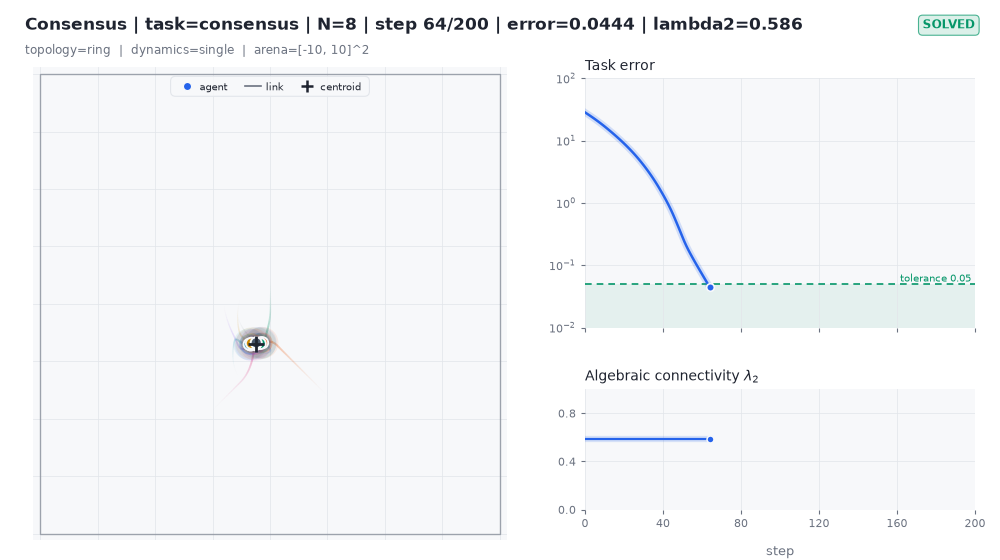
\includegraphics[width=\figwidth]{consensus.png}
  \caption{Consensus (rendezvous) of 8 single integrators on a ring, solved at
    step 64 by the Laplacian controller. The agents have gathered at the
    centroid; the task error has fallen below the tolerance and $\lambda_2$ of
    the static ring is constant.}
  \label{fig:consensus}
\end{figure}

\begin{figure}[htbp]
  \centering
  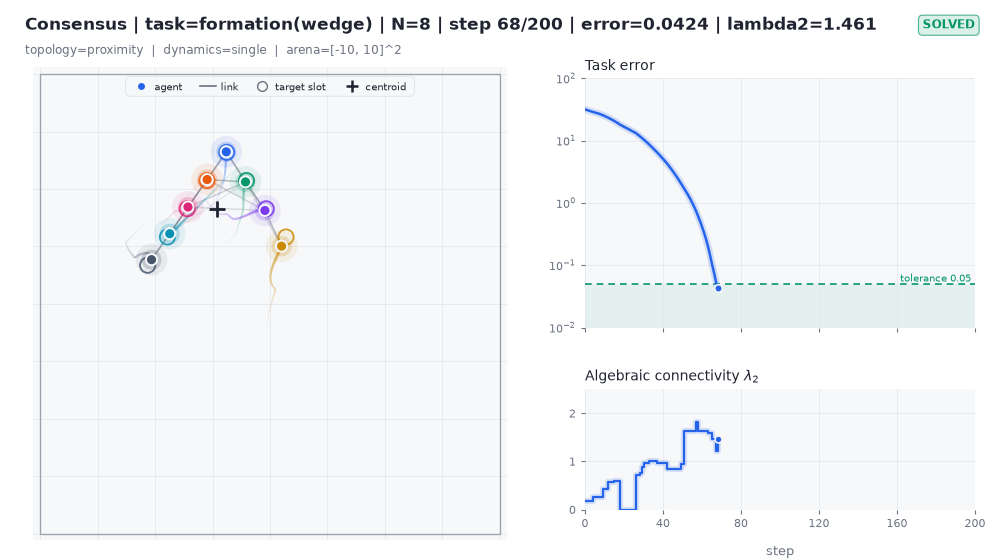
\includegraphics[width=\figwidth]{formation.png}
  \caption{Wedge formation of 8 agents on a proximity graph, solved at step 68.
    Hollow markers are the formation slots around the centroid; $\lambda_2$
    changes as links appear and disappear and drops to zero while the graph is
    disconnected.}
  \label{fig:formation}
\end{figure}

% ---------------------------------------------------------------------------
\section{Registered ids}\label{sec:consensus-ids}

\begin{table}[!htbp]
  \centering\small
  \caption{Registered ids of the consensus environment.}
  \label{tab:consensus-ids}
  \begin{tabular}{@{}lll@{}}
    \toprule
    Id & Class & Configuration \\
    \midrule
    \envid{Consensus-v0} & \code{ConsensusEnv} & defaults (rendezvous, 8 agents on a ring) \\
    \envid{Formation-v0} & \code{ConsensusEnv} & \code{task="formation"} (circle of radius 3) \\
    \bottomrule
  \end{tabular}
\end{table}

Table~\ref{tab:consensus-ids} lists the two ids. Keyword arguments of
\code{env\_lib.make} override the registered configuration, for example \code{env\_lib.make("Formation-v0", formation\_shape="wedge",
topology="proximity")}.

% ---------------------------------------------------------------------------
\section{Usage}\label{sec:consensus-usage}

\begin{pycode}
import env_lib

env = env_lib.make("Formation-v0", formation_shape="wedge",
                   topology="proximity", dynamics="double")
core = env.unwrapped
obs, info = env.reset(seed=0)                 # obs: (8, 36), K = 6 slots
layout = core.observation_layout
n, k = core.n_agents, core.max_neighbors
slots = obs[:, layout["neighbors"]].reshape(n, k, 5)   # neighbour slots
episode_return = 0.0
while True:
    action = core.laplacian_policy(gain=1.0)  # u = -gain L (x - d) - k_v v
    obs, reward, terminated, truncated, info = env.step(action)
    episode_return += reward
    if terminated or truncated:
        break
print(info["step"], info["error"], info["success"], episode_return)
env.close()
\end{pycode}

The example script compares random actions with the Laplacian controller and
records the controller:

\begin{shellcode}
python examples/environments/consensus_demo.py
python examples/environments/consensus_demo.py --task formation --save renders/formation.gif
python examples/environments/consensus_demo.py --task formation --shape wedge \
    --topology proximity --dynamics double --save renders/wedge.gif
\end{shellcode}

% ---------------------------------------------------------------------------
\section{Native vector environment}\label{sec:consensus-vector}

\code{env\_lib.make\_vec("Consensus-v0", B)} and \code{make\_vec("Formation-v0", B)}
return a \code{ConsensusVectorEnv}, which simulates $B$ copies with the same
array kernels as the single environment. It takes the constructor arguments of
\code{ConsensusEnv} plus \code{num\_envs} and \code{autoreset\_mode}, supports
every task, topology (proximity graphs are rebuilt per copy and step),
dynamics and formation shape, and returns observations of shape
$(B, N, d)$, team rewards of shape $(B,)$ and batched info arrays with a
leading $B$ axis. Each copy reproduces a single environment started from the
same state bit for bit:

\begin{pycode}
import numpy as np
import env_lib

envs = env_lib.make_vec("Formation-v0", num_envs=4)
obs, _ = envs.reset(seed=0)                     # (4, 8, 16)
single = env_lib.make("Formation-v0").unwrapped
first, _ = single.reset(options={"positions": envs.unwrapped.positions[0]})
assert np.array_equal(first, obs[0])

action = envs.unwrapped.laplacian_policy()      # batched baseline, (4, 8, 2)
obs, reward, terminated, truncated, info = envs.step(action)
assert np.array_equal(single.step(action[0])[0], obs[0])
\end{pycode}

\code{reset(options=...)} accepts \code{"positions"} and \code{"velocities"}
either for all copies (shape $(N, 2)$) or per copy (shape $(B, N, 2)$), and
combines with \code{"reset\_mask"}. Erdos-Renyi graphs are sampled once per
copy from \code{numpy.random.default\_rng(graph\_seed)}; copy 0 has the graph of
a single environment with the same \code{graph\_seed}. The default
\code{max\_neighbors} is then the maximum degree over all copies, so pass
\code{max\_neighbors} explicitly when observations must have the same width as
a single environment's. \code{render()} draws copy 0. Chapter~\ref{chap:workflow}
covers autoreset modes, seeding and throughput.

\section{Reproducibility and performance}\label{sec:consensus-perf}

The initial positions and the process noise are drawn from
\code{self.np\_random}, seeded by \code{reset(seed=...)}. The Erd\H{o}s--R\'enyi
graph is sampled once at construction from \code{graph\_seed}; pass a seed to
obtain the same graph (and observation size) in every instance, for example in
vectorised training environments.

Measured on the development machine without rendering, a step takes about
0.1\,ms with the default 8 agents and 0.18\,ms for a grid formation of 32
agents on a proximity graph. Rendering an \code{"rgb\_array"} frame takes
about 16--21\,ms.

\endgroup

\chapter{Power Grid Frequency Control}\label{chap:power_grid}

% Placeholder: written in the 1.1 update.

\chapter{Vehicle Platoon Control}\label{chap:platoon}

% Placeholder: written in the 1.1 update.

% ---------------------------------------------------------------------------
% AJLATT: active joint localisation and target tracking
% ---------------------------------------------------------------------------
\begingroup
% Line breaking for paragraphs with long, unbreakable identifiers (local to
% this chapter): allow looser lines instead of overfull ones.
\setlength{\emergencystretch}{3em}\tolerance=1000
\chapter{AJLATT: Active Joint Localisation and Target Tracking}\label{chap:ajlatt}

In AJLATT a team of mobile robots with range-bearing sensors has to localise
itself and track a moving target on an occupancy grid map. Every robot runs an
estimator for its own pose and for the target; estimates are exchanged within a
limited communication range and fused with covariance intersection. The robots
choose their velocities, and the reward drives the team to keep the target and
its own poses well estimated while avoiding obstacles, the map border and each
other. The environment is used to study active perception and
information-driven control, cooperative localisation and distributed target
tracking, and multi-agent reinforcement learning with continuous actions,
partial observability and safety constraints.

The main entry points are exported by \code{env\_lib.ajlatt\_env}:
\begin{description}[style=nextline,leftmargin=3.9cm]
  \item[\code{AJLATTEnv}] the Gymnasium environment with joint multi-agent
    spaces (also available as \code{env\_lib.AJLATTEnv});
  \item[\code{AJLATTConfig}] a validated dataclass holding every parameter;
  \item[\code{TeamRewardWrapper}] a scalar-reward view for single-agent
    algorithms;
  \item[\code{make}] the backwards-compatible factory accepting the original
    keyword names;
  \item[\code{maps}] occupancy maps, the map builder and map plotting
    (Section~\ref{sec:ajlatt-maps}).
\end{description}

% ---------------------------------------------------------------------------
\section{Scenario and motion model}\label{sec:ajlatt-scenario}

The team consists of \code{num\_robots} robots (default 4) and
\code{num\_targets} targets (default 1). Target 0 moves according to a target
policy (Section~\ref{sec:ajlatt-target}); further targets are static landmarks
whose positions are estimated in 2-D. One step lasts $\Delta t$ =
\code{sampling\_period} (0.5\,s), so the default episode of 120 steps covers
60\,s. Robots and the target follow the unicycle model
\begin{equation}
  \begin{bmatrix} p_x \\ p_y \\ \theta \end{bmatrix}_{k+1}
  = \begin{bmatrix} p_x \\ p_y \\ \theta \end{bmatrix}_{k}
  + \begin{bmatrix} v\,\Delta t \cos\theta_k \\ v\,\Delta t \sin\theta_k \\ \omega\,\Delta t \end{bmatrix},
  \label{eq:ajlatt-unicycle}
\end{equation}
with the heading wrapped to $[-\pi, \pi)$. The true robot poses are propagated
with noisy velocities $v \sim \mathcal{N}(v_{\mathrm{cmd}}, \sigma_v^2)$,
$\omega \sim \mathcal{N}(\omega_{\mathrm{cmd}}, \sigma_\omega^2)$, where
$(\sigma_v, \sigma_\omega)$ = (\code{sigma\_vR}, \code{sigma\_wR}); with
\code{process\_noise\_fixed=False} the noise scales with the speed,
$\sigma_v = \sigma/\sqrt{2}$ and $\sigma_\omega = 2\sqrt{2}\,\sigma$ with
$\sigma$ = \code{sigmapR}$\,\cdot v_{\mathrm{cmd}}$. The target moves exactly
with the command of its policy, while the robots predict their target beliefs
with a noisy copy of that command (\code{sigma\_vT}, \code{sigma\_wT}, or
\code{sigmapT}$\,\cdot$\code{target\_linear\_velocity} in the speed-dependent
case).

% ---------------------------------------------------------------------------
\section{Sensing, communication and estimation}\label{sec:ajlatt-estimation}

\paragraph{Beliefs.} Robot $i$ keeps a Gaussian belief
$(\hat x_i, P_i)$ of its own pose and a belief
$(\hat x^{T}_{i,t}, P^{T}_{i,t})$ of every target $t$ (a pose for target 0, a
position for landmarks). At reset the means are drawn around the initial poses
with the initial covariances: $P_i$ = \code{robot\_init\_cov[i]}$\,I$ with
heading variance $10^{-3}$, and $P^T_{i,t}$ = \code{target\_init\_cov[t]}$\,I$
with heading variance 0.1 for target 0.

\paragraph{Prediction.} Every belief is predicted with an extended Kalman filter
step for \eqref{eq:ajlatt-unicycle}:
\begin{equation}
  \hat x \leftarrow f(\hat x, u), \qquad
  P \leftarrow \Phi P \Phi^\top + G Q G^\top, \qquad
  Q = \operatorname{diag}(\sigma_v^2, \sigma_\omega^2),
\end{equation}
where $\Phi$ is the Jacobian of the motion with respect to the pose and
$G = \Delta t \bigl[\begin{smallmatrix} \cos\theta & 0 \\ \sin\theta & 0 \\ 0 & 1 \end{smallmatrix}\bigr]$
its Jacobian with respect to the velocity noise.

\paragraph{Measurements.} Robot $\ell$ measures the range and bearing
$z = (\rho, \beta)$ of another robot or a target $j$ when
\code{sensor\_r\_min} $< \rho <$ \code{sensor\_r\_max},
$|\beta| \le$ \code{fov}$/2$, the straight line between the two (true)
positions does not cross an occupied cell of the grid (Bresenham ray casting),
and robot $\ell$'s estimated position lies inside the map. The measurement noise
has standard deviations $\sigma_\rho$ = \code{sigma\_p}$\,\cdot\rho$ (with
\code{range\_noise\_proportional=True}) or \code{sigma\_r}, and
$\sigma_\beta$ = \code{sigma\_th}. All three default to zero: by default the
measurements are exact, and the uncertainty of the estimates stems from the
motion noise and from the uncertainty of the measured party's own estimate.

\paragraph{Communication.} Robots closer than \code{commu\_r\_max} (true
distance) are neighbours; the neighbour set $\mathcal{N}_i$ of robot $i$
includes $i$ itself.

\paragraph{Update.} With \code{use\_update=True} (default) the robots are
processed one after another in index order, and each update is applied in place,
so later robots use the updated beliefs of earlier ones:
\begin{enumerate}
  \item \emph{Self-localisation.} Every measurement $z$ of an entity $j$ with
        belief $(\hat x_j, P_j)$ contributes the information pair
        \begin{equation*}
          S = H_i^\top W H_i, \qquad
          y = H_i^\top W \bigl(z - \hat z + H_i \hat x_i\bigr), \qquad
          W = \bigl(R + H_j P_j H_j^\top\bigr)^{-1},
        \end{equation*}
        where $\hat z$ is the predicted measurement and $H_i$, $H_j$ are the
        Jacobians of the range-bearing model with respect to the observer and
        the observed pose. These pairs and the prior
        $(P_i^{-1}, P_i^{-1}\hat x_i)$ are fused by covariance intersection.
  \item \emph{Target tracking.} For each target, the measurements of all
        neighbours $r \in \mathcal{N}_i$ that detect it contribute analogous
        information pairs (with the roles of observer and target exchanged);
        these are fused by covariance intersection in information form. The
        neighbours' prior beliefs of the target are fused in the same way, and
        the two results are combined by a final covariance intersection. If no
        neighbour detects the target, robot $i$'s belief is the fusion of the
        neighbours' priors.
\end{enumerate}
With \code{use\_update=False} the robots only dead-reckon.

\paragraph{Covariance intersection.} Given information pairs
$(S_k, y_k)$, $k = 1, \dots, K$, covariance intersection chooses weights $c$ on
the probability simplex that minimise the trace of the fused covariance,
\begin{equation}
  c^\star = \operatorname*{arg\,min}_{c \ge 0,\; \sum_k c_k = 1}
    \operatorname{tr}\Bigl(\bigl(\textstyle\sum_k c_k S_k\bigr)^{-1}\Bigr),
  \qquad
  P = \Bigl(\sum_k c^\star_k S_k\Bigr)^{-1},\quad
  \hat x = P \sum_k c^\star_k y_k .
\end{equation}
The fused estimate is consistent without knowledge of the correlations between
the sources. The solver is chosen with \code{ci\_solver}:
\code{"newton"} (default) is an active-set projected Newton method with the
analytic gradient $g_k = -\operatorname{tr}(P S_k P)$ and Hessian
$H_{kl} = 2 \operatorname{tr}(P S_k P S_l P)$; its objective is never worse than
that of \code{"slsqp"}, the original solver (SciPy SLSQP with finite-difference
gradients), which reproduces trajectories of the implementation before
version 1.0 to about $10^{-6}$.

% ---------------------------------------------------------------------------
\section{Spaces}\label{sec:ajlatt-spaces}

\paragraph{Action.} \code{Box} of shape \code{(num\_robots, 2)}, one command
$(v, \omega)$ per robot with $0 \le v \le v_{\max}$ and
$|\omega| \le \omega_{\max}$, where $v_{\max}$ =
\code{max\_linear\_velocity} (default 2\,m/s) and $\omega_{\max}$ =
\code{max\_angular\_velocity} (default $\pi/4$\,rad/s). The per-robot space
is \code{env.single\_action\_space}. Actions are not clipped unless
\code{clip\_actions=True} (the original environment did not clip). NumPy arrays
and tensors are accepted; rows beyond \code{num\_robots} are ignored with a
warning, and fewer rows raise \code{ValueError}.

\paragraph{Observation.} \code{Box} of shape \code{(num\_robots, obs\_dim)}
with $\text{obs\_dim} = 7 + 4(n_R - 1) + 5$ for $n_R$ robots (24 for the
default team); the per-robot space is \code{env.single\_observation\_space}.
Row $i$ is computed from robot $i$'s beliefs; positions and headings of other
entities are expressed in robot $i$'s estimated body frame.
\code{env.observation\_layout()} returns the slices of
Table~\ref{tab:ajlatt-obs}.

\begin{table}[htbp]
  \centering\small
  \caption{AJLATT observation of robot $i$ ($n = 6 + 4(n_R - 1)$).}
  \label{tab:ajlatt-obs}
  \begin{tabularx}{\textwidth}{@{}>{\raggedright\arraybackslash}p{0.33\textwidth}l>{\raggedright\arraybackslash}X@{}}
    \toprule
    Key of \code{observation\_layout()} & Columns & Content \\
    \midrule
    \code{target\_relative\_position} & \code{0:2} & believed target position in the robot frame \\
    \code{target\_relative\_heading} & \code{2} & believed target heading minus own heading \\
    \code{target\_velocity} & \code{3:5} & commanded target velocity $(v, \omega)$ of the last step (zero after reset) \\
    \code{target\_cov\_trace} & \code{5} & $\operatorname{tr} P^T_{i,0}$ \\
    \code{neighbours} & \code{6:n} & for every other robot, in index order: relative $x$, relative $y$, relative heading (estimates), trace of its covariance \\
    \code{closest\_obstacle} & \code{n:n+2} & range and bearing of the closest obstacle cell within the field of view and sensor range; $(r_{\max}, \pi)$ if none; zeros while the robot is within \code{obstacle\_sensing\_margin} of the map border \\
    \code{self\_pose} & \code{n+2:n+5} & own pose estimate $(x, y, \theta)$ in the map frame \\
    \code{self\_cov\_trace} & \code{n+5} & $\operatorname{tr} P_i$ \\
    \bottomrule
  \end{tabularx}
\end{table}

% ---------------------------------------------------------------------------
\section{Reward and episode end}\label{sec:ajlatt-reward}

\code{step()} returns the per-robot rewards as an array of shape
\code{(num\_robots,)}. They are built from the tracking cost $c_i$ and the
penalty $p_i$ of robot $i$ in the step,
\begin{equation}
  c_i = w_T \operatorname{tr} P^T_{i,0} + w_R \operatorname{tr} P_i, \qquad
  p_i = \beta_B\, \mathbf{1}_{\mathrm{border}}(i)
        + \beta_O\, \mathbf{1}_{\mathrm{obstacle}}(i)
        + \beta_M\, \mathbf{1}_{\mathrm{mutual}}(i),
  \label{eq:ajlatt-cost}
\end{equation}
and, in the default \code{reward\_mode="cost"} (the original reward),
\begin{equation}
  r_i = -c_i - p_i,
  \label{eq:ajlatt-reward}
\end{equation}
with $w_T$ = \code{target\_cov\_weight} (10), $w_R$ = \code{robot\_cov\_weight}
(5) and the penalties
\begin{itemize}
  \item $\beta_B$ = \code{boundary\_penalty} (20) when the estimated position
        lies within 0.1\,m of the map border or outside the map;
  \item otherwise $\beta_O$ = \code{obstacle\_penalty} (1.3) when an obstacle
        cell is closer to the estimated pose than
        \code{obstacle\_collision\_distance} (0.2\,m, searched in all
        directions up to \code{sensor\_r\_max}); this also sets the robot's
        collision flag;
  \item $\beta_M$ = \code{mutual\_collision\_penalty} (0.5) when another
        robot's estimated position is closer than
        \code{mutual\_collision\_distance} (0.4\,m).
\end{itemize}
The team reward is $\sum_i r_i$ (\code{info["team\_reward"]}), and
\code{info["tracking\_cost"]} holds $c_i$ for evaluations that do not depend
on the reward settings.

\paragraph{Reward settings.} Four configuration fields change the reward
(Table~\ref{tab:ajlatt-reward-settings}); they are applied in the order of the
table.

\begin{table}[htbp]
  \centering\small
  \caption{Reward settings of AJLATT (defaults first; the defaults give the
    original reward \eqref{eq:ajlatt-reward}).}
  \label{tab:ajlatt-reward-settings}
  \begin{tabularx}{\textwidth}{@{}p{4.2cm}>{\raggedright\arraybackslash}X@{}}
    \toprule
    Setting & Effect \\
    \midrule
    \code{reward\_mode="cost"} & $r_i = -c_i - p_i$: every reward is negative. \\
    \code{reward\_mode="bounded"} & $r_i = e^{-c_i/\sigma} - p_i/\sigma$ with
      $\sigma$ = \code{cost\_scale} (20): at most 1, positive while the robot
      tracks well, so a collision that ends the episode forfeits the rewards of
      the remaining steps. \\
    \code{terminate\_on\_collision} (\code{True}) & An obstacle collision ends
      the robot's episode (\code{terminated[i]}); with \code{False} the
      collision is only penalised and the episode continues. \\
    \code{collision\_termination\_penalty} (0) & Subtracted from $r_i$ on the
      step a collision ends robot $i$'s episode. \\
    \code{team\_reward\_weight} $w$ (0) & $r_i \leftarrow (1-w)\, r_i + w\,
      \frac{1}{n_R}\sum_j r_j$: 0 keeps individual rewards, 1 gives every robot
      the team mean; the team sum is unchanged. \\
    \bottomrule
  \end{tabularx}
\end{table}

\paragraph{Choosing the settings.} With the defaults every reward is negative
and the first collision ends the episode (in the team view of
\code{TeamRewardWrapper} and \code{env\_lib.make\_vec}), so a team can raise its
return by colliding early: on 64 seeded episodes random actions reach $-627$
in 16 steps, the classical controller $-7{,}090$ in 115. The registered id
keeps this reward for compatibility, and \code{env-lib describe} prints a
caution. For learning, use \code{reward\_mode="bounded"} (random 39.9,
controller 223.6) or \code{terminate\_on\_collision=False} (random
$-34{,}273$, controller $-7{,}415$), or a
\code{collision\_termination\_penalty} larger than the cost of an episode.

\begin{pycode}
import env_lib

env = env_lib.make("AJLATT-v0", terminate_on_collision=False)   # penalised, not stopped
env = env_lib.make("AJLATT-v0", reward_mode="bounded", team_reward_weight=0.5)
\end{pycode}

\paragraph{Episode end.} \code{terminated} is a boolean array of shape
\code{(num\_robots,)} holding the obstacle collision flags (all \code{False}
with \code{terminate\_on\_collision=False}). If an estimator diverges
(non-finite covariance) all flags are set, a \code{RuntimeWarning} is issued and
\code{info["numerical\_error"]} is \code{True}. \code{truncated} is a
\code{bool}, set after \code{max\_episode\_steps} steps. The environment keeps
simulating after a collision flag; whether a flag ends the episode is left to
the caller (\code{record\_episode} and \code{TeamRewardWrapper} use
\code{any(terminated)}).

% ---------------------------------------------------------------------------
\section{Configuration}\label{sec:ajlatt-config}

\code{AJLATTEnv(config=None, render\_mode=None, **overrides)} takes an
\code{AJLATTConfig} and/or individual fields as keyword arguments, which are
applied on top of \code{config}. Unknown field names raise \code{TypeError}.

\begin{pycode}
from env_lib import AJLATTConfig, AJLATTEnv

env = AJLATTEnv(map_name="obstacles05", num_robots=3)   # fields as keywords
config = AJLATTConfig(map_name="obstacles04", sensor_r_max=5.0, fov=120.0)
env = AJLATTEnv(config, render_mode="rgb_array")
env = AJLATTEnv(config.replace(ci_solver="slsqp"))              # validated copy
\end{pycode}

\code{AJLATTConfig} validates its values on construction (for example
\code{0 <= sensor\_r\_min < sensor\_r\_max}, \code{0 < fov <= 360}, non-negative
noise levels, enough initial poses and covariances for the team) and offers
\code{replace(**changes)}, \code{to\_dict()} and \code{from\_dict(data)}, the
property \code{observation\_dim}, and \code{from\_kwargs(strict=True, **kwargs)},
which also accepts the legacy names of Table~\ref{tab:ajlatt-legacy} (as do
\code{AJLATTEnv}, \code{env\_lib.ajlatt\_env.make} and the callable module
\code{env\_lib.ajlatt\_env}). All
fields are listed in Table~\ref{tab:ajlatt-params}.

\begingroup\small
\setlength{\LTcapwidth}{\textwidth}
\begin{longtable}{@{}>{\raggedright\arraybackslash}p{0.32\textwidth}>{\raggedright\arraybackslash}p{0.18\textwidth}>{\raggedright\arraybackslash}p{0.44\textwidth}@{}}
  \caption{Fields of \code{AJLATTConfig} (keyword arguments of \code{AJLATTEnv}).}\label{tab:ajlatt-params}\\
  \toprule
  Field & Default & Description \\
  \midrule
  \endfirsthead
  \toprule
  Field & Default & Description \\
  \midrule
  \endhead
  \bottomrule
  \endfoot
  \multicolumn{3}{@{}l}{\textit{Scenario}} \\
  \code{map\_name} & \code{"obstacles04"} & Bundled map name or path to a user map (Section~\ref{sec:ajlatt-maps}). \\
  \code{num\_robots} & \code{4} & Team size $n_R$ ($\ge 1$). \\
  \code{num\_targets} & \code{1} & Number of targets; target 0 moves, the others are static landmarks. \\
  \code{max\_episode\_steps} & \code{120} & Episode length; reaching it sets \code{truncated}. \\
  \code{sampling\_period} & \code{0.5} & Duration $\Delta t$ of one step in seconds. \\
  \code{margin2wall} & \code{1.0} & Safety margin of the map queries \code{in\_bound} and \code{is\_collision}. \\
  \code{robot\_init\_pose} & six poses & $(x, y, \theta)$ per robot; the first four defaults are $(7.5, 12.5, 0)$, $(7.5, 10.5, 0)$, $(10, 12.5, 0)$, $(10, 10.5, 0)$. \\
  \code{target\_init\_pose} & 13 poses & $(x, y, \theta)$ per target; target 0 starts at $(10.5, 11.5, 0)$. \\
  \code{robot\_init\_cov} & \code{(0.1,) * 6} & Initial position variance per robot. \\
  \code{target\_init\_cov} & \code{(1.0,) + (10.0,) * 10} & Initial position variance per target. \\
  \multicolumn{3}{@{}l}{\textit{Sensing and communication}} \\
  \code{sensor\_r\_min} & \code{0.0} & Minimum sensing range (m). \\
  \code{sensor\_r\_max} & \code{3.0} & Maximum sensing range (m); also the range of the obstacle reading. \\
  \code{fov} & \code{180.0} & Field of view in degrees, centred on the heading. \\
  \code{sigma\_p} & \code{0.0} & Range noise as a fraction of the range (proportional mode). \\
  \code{sigma\_r} & \code{0.0} & Absolute range noise (m) when \code{range\_noise\_proportional=False}. \\
  \code{sigma\_th} & \code{0.0} & Bearing noise (rad). \\
  \code{range\_noise\_proportional} & \code{True} & Use \code{sigma\_p} instead of \code{sigma\_r}. \\
  \code{use\_update} & \code{True} & Run measurement updates (\code{False}: dead reckoning only). \\
  \code{commu\_r\_max} & \code{6.0} & Communication range (m). \\
  \code{ci\_solver} & \code{"newton"} & Covariance-intersection solver, \code{"newton"} or \code{"slsqp"}. \\
  \multicolumn{3}{@{}l}{\textit{Motion noise}} \\
  \code{process\_noise\_fixed} & \code{True} & Fixed velocity noise; \code{False} scales it with the speed. \\
  \code{sigmapR} & \code{0.1} & Robot noise factor in the speed-dependent mode. \\
  \code{sigma\_vR} & \code{0.1} & Robot linear-velocity noise (m/s). \\
  \code{sigma\_wR} & $0.5\pi/180$ & Robot angular-velocity noise (rad/s, 0.5 degrees/s). \\
  \code{sigmapT} & \code{0.1} & Target noise factor in the speed-dependent mode. \\
  \code{sigma\_vT} & \code{0.2} & Target linear-velocity noise used by the estimators (m/s). \\
  \code{sigma\_wT} & $0.5\pi/180$ & Target angular-velocity noise used by the estimators (rad/s). \\
  \multicolumn{3}{@{}l}{\textit{Target motion}} \\
  \code{target\_policy} & \code{"auto"} & Target policy (Table~\ref{tab:ajlatt-target}). \\
  \code{target\_linear\_velocity} & \code{0.3} & Speed of the \code{"sine"} policy; also scales the speed-dependent target noise. \\
  \code{target\_omega\_bound} & $\pi/4$ & Turn-rate bound of the \code{"random"} policy. \\
  \code{k\_theta} & \code{0.5} & Heading gain of the \code{"sine"} and \code{"waypoints"} policies. \\
  \code{k\_p} & \code{1.0} & Kept for compatibility; currently unused. \\
  \multicolumn{3}{@{}l}{\textit{Actions}} \\
  \code{max\_linear\_velocity} & \code{2.0} & Upper bound of $v$ (m/s); the lower bound is 0. \\
  \code{max\_angular\_velocity} & $\pi/4$ & Bound of $|\omega|$ (rad/s). \\
  \code{clip\_actions} & \code{False} & Clip actions to the action space. \\
  \multicolumn{3}{@{}l}{\textit{Rewards and termination}} \\
  \code{target\_cov\_weight} & \code{10.0} & Weight $w_T$ of the target covariance trace. \\
  \code{robot\_cov\_weight} & \code{5.0} & Weight $w_R$ of the self-localisation covariance trace. \\
  \code{boundary\_penalty} & \code{20.0} & Penalty $\beta_B$ near or beyond the map border (0.1\,m margin). \\
  \code{obstacle\_penalty} & \code{1.3} & Penalty $\beta_O$ for an obstacle closer than \code{obstacle\_collision\_distance}. \\
  \code{obstacle\_collision\_distance} & \code{0.2} & Obstacle collision distance (m). \\
  \code{mutual\_collision\_penalty} & \code{0.5} & Penalty $\beta_M$ for robots closer than \code{mutual\_collision\_distance}. \\
  \code{mutual\_collision\_distance} & \code{0.4} & Robot-robot distance threshold (m). \\
  \code{terminate\_on\_collision} & \code{True} & End a robot's episode (\code{terminated}) at an obstacle collision; \code{False} only penalises it. \\
  \code{reward\_mode} & \code{"cost"} & \code{"cost"} or \code{"bounded"} (Table~\ref{tab:ajlatt-reward-settings}). \\
  \code{cost\_scale} & \code{20.0} & Scale $\sigma$ of the \code{"bounded"} reward. \\
  \code{collision\_termination\_penalty} & \code{0.0} & Extra penalty when a collision ends a robot's episode. \\
  \code{team\_reward\_weight} & \code{0.0} & Weight $w \in [0, 1]$ of the team mean in each robot's reward. \\
  \code{obstacle\_sensing\_margin} & \code{1.0} & Robots closer than this to the map border report a zero obstacle reading (original behaviour). \\
  \multicolumn{3}{@{}l}{\textit{Miscellaneous}} \\
  \code{seed} & \code{None} & Seed of the first \code{reset()} when none is passed. \\
\end{longtable}
\endgroup

The default poses and covariances cover up to six robots and eleven targets;
larger teams need explicit \code{robot\_init\_pose} and \code{robot\_init\_cov}
(and likewise for targets).

\begin{table}[htbp]
  \centering\small
  \caption{Legacy parameter names; each emits a \code{DeprecationWarning}.}
  \label{tab:ajlatt-legacy}
  \begin{tabularx}{\textwidth}{@{}l>{\raggedright\arraybackslash}X@{}}
    \toprule
    Legacy name & Replacement \\
    \midrule
    \code{num\_Robot}, \code{num\_Target} & \code{num\_robots}, \code{num\_targets} \\
    \code{T\_steps} & \code{max\_episode\_steps} \\
    \code{maxmum\_run} & caps \code{max\_episode\_steps} at \code{maxmum\_run + 1} \\
    \code{SIGPERCENT} & \code{range\_noise\_proportional} \\
    \code{useupdate} & \code{use\_update} \\
    \code{fix\_seed} & \code{seed} (\code{fix\_seed=True} sets \code{seed=1}) \\
    \code{render=True} & \code{render\_mode="human"} \\
    obsolete keys (\code{figID}, \code{ssh\_debug}, \code{episode\_num}, \dots) & ignored with a warning \\
    \bottomrule
  \end{tabularx}
\end{table}

\paragraph{Command-line integration.} \code{AJLATTConfig.add\_arguments(parser,
prefix="")} registers every scalar field as an option \code{-{}-<prefix><name>}
on an \code{argparse} parser, and \code{AJLATTConfig.from\_namespace(namespace,
prefix="")} builds a configuration from the parsed arguments. Training scripts
keep their own options next to the environment's:

\begin{pycode}
import argparse
from env_lib import AJLATTConfig, AJLATTEnv

parser = argparse.ArgumentParser()
parser.add_argument("--lr", type=float, default=3e-4)     # training options
AJLATTConfig.add_arguments(parser, prefix="env.")        # --env.map_name, ...
args = parser.parse_args(["--env.map_name", "obstacles05",
                          "--env.num_robots", "3"])
env = AJLATTEnv(AJLATTConfig.from_namespace(args, prefix="env."))
\end{pycode}

% ---------------------------------------------------------------------------
\section{Target motion}\label{sec:ajlatt-target}

The target policy maps the true target pose to a unicycle command. Policies are
per-environment objects that are reset with the environment's generator at
every \code{reset()}.

\begin{table}[htbp]
  \centering\small
  \caption{Target policies (\code{target\_policy}).}
  \label{tab:ajlatt-target}
  \begin{tabularx}{\textwidth}{@{}l>{\raggedright\arraybackslash}X@{}}
    \toprule
    Policy & Behaviour \\
    \midrule
    \code{"auto"} & \code{"sine"} on the map \code{empty}, \code{"waypoints"} on
      \code{obstacles04} and \code{obstacles05}, \code{"circle"} otherwise \\
    \code{"sine"} & follows the slope field $dy/dx = 5\cos x$ at speed
      \code{target\_linear\_velocity} with heading gain \code{k\_theta} until
      $x \ge 32$\,m, then circles with $v = 0.25$\,m/s on a 4\,m radius \\
    \code{"waypoints"} & proportional heading control (gain \code{k\_theta})
      towards piecewise waypoints; built-in routes for \code{obstacles04}
      (0.1\,m/s) and \code{obstacles05} (0.25\,m/s); other routes with
      \code{env\_lib.ajlatt\_env.controllers.WaypointPolicy} \\
    \code{"circle"} & constant $(v, \omega) = (0.25\,\mathrm{m/s}, 0.15\,\mathrm{rad/s})$ \\
    \code{"random"} & $v = 0.25$\,m/s and a turn rate drawn uniformly from
      $[-$\code{target\_omega\_bound}, \code{target\_omega\_bound}$]$ at every step \\
    \code{"static"} & the target does not move \\
    \bottomrule
  \end{tabularx}
\end{table}

% ---------------------------------------------------------------------------
\section{Info dictionary and episode statistics}\label{sec:ajlatt-info}

\begin{table}[htbp]
  \centering\small
  \caption{AJLATT info dictionary ($n_R$ = \code{num\_robots}).}
  \label{tab:ajlatt-info}
  \begin{tabularx}{\textwidth}{@{}l>{\raggedright\arraybackslash}X@{}}
    \toprule
    Key & Content \\
    \midrule
    \code{agent\_rewards} & \code{float64} array $(n_R,)$, equal to the returned rewards (zeros at reset) \\
    \code{team\_reward} & sum of the per-robot rewards \\
    \code{collisions} & boolean array $(n_R,)$: obstacle collisions in this step \\
    \code{episode\_collisions} & integer array $(n_R,)$: number of border, obstacle and robot-robot penalty events in the episode \\
    \code{target\_observed} & boolean array $(n_R,)$: robot measured target 0 in this step \\
    \code{communication} & boolean matrix $(n_R, n_R)$: communication links, including self-loops \\
    \code{robot\_cov\_trace} & array $(n_R,)$: $\operatorname{tr} P_i$ \\
    \code{target\_cov\_trace} & array $(n_R,)$: $\operatorname{tr} P^T_{i,0}$ \\
    \code{tracking\_cost} & array $(n_R,)$: tracking cost $c_i$ of \eqref{eq:ajlatt-cost} (\code{step()} only) \\
    \code{step} & number of steps taken \\
    \code{numerical\_error} & \code{True} if an estimator diverged (\code{step()} only) \\
    \bottomrule
  \end{tabularx}
\end{table}

\code{env.episode\_statistics()} returns per-step traces of the current
episode as arrays of shape \code{(steps + 1, num\_robots)}, starting with the
state after reset: \code{robot\_cov\_trace}, \code{target\_cov\_trace},
\code{robot\_error} and \code{target\_error} (Euclidean position errors of the
robots' own and target beliefs) and \code{reward}. The traces are cleared at
every reset.

% ---------------------------------------------------------------------------
\section{Team reward wrapper and legacy factory}\label{sec:ajlatt-wrapper}

\code{TeamRewardWrapper(env)} returns the team reward $\sum_i r_i$ as a
\code{float} and \code{any(terminated)} as a \code{bool}, for algorithms that
expect scalar values. The per-robot values remain available in the info
dictionary under \code{"agent\_rewards"} and \code{"agent\_terminated"}.

\begin{pycode}
from env_lib import AJLATTEnv
from env_lib.ajlatt_env import TeamRewardWrapper

env = TeamRewardWrapper(AJLATTEnv(map_name="obstacles04"))
obs, info = env.reset(seed=1)
obs, reward, terminated, truncated, info = env.step(env.action_space.sample())
\end{pycode}

The original factory remains available for existing code:
\code{env\_lib.ajlatt\_env.make(**kwargs)}, or the callable module
\code{env\_lib.ajlatt\_env(num\_Robot=4, T\_steps=100)}. It translates the legacy
names of Table~\ref{tab:ajlatt-legacy}, ignores unknown keys with a warning and
maps \code{render=True} to \code{render\_mode="human"}. New code should create
\code{AJLATTEnv} directly.

% ---------------------------------------------------------------------------
\section{Maps}\label{sec:ajlatt-maps}

The subpackage \code{env\_lib.ajlatt\_env.maps} contains the occupancy maps and
the tools to create and inspect them.

\subsection{Bundled maps}\label{sec:ajlatt-bundled-maps}

\code{available\_maps()} lists the bundled maps (Table~\ref{tab:ajlatt-maps});
\code{ajlatt-plot-map -{}-list} prints the same list. All maps start at the
origin (\code{mapmin} $= (0, 0)$). Figure~\ref{fig:ajlatt-map} shows
\code{obstacles05}.

\begin{table}[htbp]
  \centering\small
  \caption{Bundled maps. Size in cells ($n_x \times n_y$) and metres.}
  \label{tab:ajlatt-maps}
  \begin{tabularx}{\textwidth}{@{}>{\raggedright\arraybackslash}p{0.34\textwidth}lll>{\raggedright\arraybackslash}X@{}}
    \toprule
    Map & Cells & Cell size & Extent & Notes \\
    \midrule
    \code{obstacles} & $51 \times 51$ & 0.5\,m & 25.5\,m & \\
    \code{obstacles02}, \code{obstacles07}, \code{obstacles07-02}, \code{obstacles08} & $181 \times 181$ & 0.2\,m & 36.2\,m & \\
    \code{obstacles03} & $102 \times 102$ & 0.2\,m & 20.4\,m & \\
    \code{obstacles04} & $181 \times 181$ & 0.2\,m & 36.2\,m & default; waypoint route \\
    \code{obstacles05} & $181 \times 181$ & 0.4\,m & 72.4\,m & waypoint route \\
    \code{obstacles06}, \code{obstacles06-02}, \code{obstacles06-03}, \code{obstacles08-02} & $181 \times 181$ & 0.1\,m & 18.1\,m & \\
    \code{example\_complete\_map}, \code{sample\_map\_config} & $181 \times 181$ & 0.4\,m & 72.4\,m & map builder examples \\
    \code{empty} & $82 \times 62$ & 0.5\,m & $41 \times 31$\,m & no obstacles; sine target policy \\
    \code{empty05} & $181 \times 181$ & 0.4\,m & 72.4\,m & no obstacles \\
    \code{emptySmall} & $135 \times 135$ & 0.2\,m & 27\,m & no obstacles \\
    \code{emptySmall05} & $65 \times 65$ & 0.4\,m & 26\,m & no obstacles \\
    \code{dynamic\_map}, \code{dynamic\_map\_2} & $181 \times 181$ & 0.4\,m & 72.4\,m & obstacles resampled at every reset \\
    \bottomrule
  \end{tabularx}
\end{table}

\begin{figure}[htbp]
  \centering
  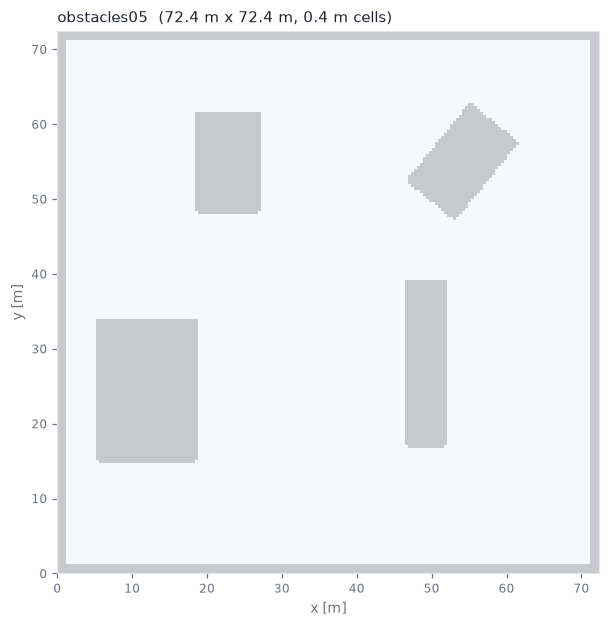
\includegraphics[width=0.55\textwidth]{map_obstacles05.png}
  \caption{The bundled map \code{obstacles05} ($72.4 \times 72.4$\,m,
    0.4\,m cells) plotted with \code{ajlatt-plot-map obstacles05}; occupied
    cells are grey, including the one-cell wall around the map.}
  \label{fig:ajlatt-map}
\end{figure}

\subsection{Map files}\label{sec:ajlatt-map-format}

A static map consists of two files with the same name:
\begin{itemize}
  \item \code{<name>.yaml}, the header, with the keys \code{mapdim}
        ($[n_x, n_y]$, cells along $x$ and $y$), \code{mapres} (cell size
        $[r_x, r_y]$ in metres), \code{mapmin} and \code{mapmax} (corners of the
        map in metres) and optionally \code{origin}. Further keys written by
        older tools or the map builder (\code{datatype}, \code{mappath},
        \code{origincells}, \code{storage}, the embedded specification) are
        ignored by the loader.
  \item \code{<name>.cfg}, the occupancy grid as whitespace-separated numbers,
        one text row per grid row: $n_y$ rows of $n_x$ values, where row 0 is
        the bottom row ($y$ = \code{mapmin}) and 1 marks an occupied cell.
\end{itemize}
Cell $(c_x, c_y)$ has its centre at $(c + 0.5)\,r + $\code{mapmin}. A grid with
fewer cells than its header declares is padded with occupied cells and a
warning. An empty (zero-byte) \code{.cfg} file denotes an obstacle-free map in
which only the boundary blocks rays; a map whose name contains \code{empty} may
omit the file altogether, while a missing grid for any other static map raises
\code{FileNotFoundError}. A dynamic map has only a header, which defines
\code{submaporigin} (four $(\text{row}, \text{column})$ cell anchors, flattened
to eight numbers) and \code{lib\_path} (a directory of \code{.npy} obstacle
masks relative to the header).

To use your own map, pass its path to \code{map\_name}, with or without the
\code{.yaml} suffix, for example \code{AJLATTEnv(map\_name="maps/my\_map")};
the grid file must sit next to the header. Check that the default initial poses
(Table~\ref{tab:ajlatt-params}) are free cells of the map, or pass
\code{robot\_init\_pose} and \code{target\_init\_pose}.

\subsection{Map API}\label{sec:ajlatt-map-api}

\begin{itemize}
  \item \code{load\_grid\_map(name\_or\_path, margin2wall=0.5)} returns a
        \code{GridMap}, or a \code{DynamicMap} for a header with
        \code{submaporigin} and no grid. \code{load\_map(name)} returns
        \code{(occupancy, mapmin, mapmax)} for plotting, and
        \code{resolve\_map\_path(name)} the file path without suffix.
  \item \code{GridMap} holds the grid as \code{map} (shape $(n_y, n_x)$,
        \code{None} for empty maps) together with \code{mapdim}, \code{mapres},
        \code{mapmin} and \code{mapmax}; its queries are listed in
        Table~\ref{tab:ajlatt-gridmap}. \code{GridMap.from\_array(occupancy,
        mapmin=(0, 0), mapres=0.4)} builds a map from an array of shape
        $(n_y, n_x)$.
  \item \code{DynamicMap.generate\_map(chosen\_idx=None, rot\_angs=None,
        rng=None)} places four distinct obstacles from its library at the four
        anchors, each rotated by a random multiple of 18 degrees, and closes the
        border. The environment calls it with its own generator at every reset.
\end{itemize}

\begin{table}[htbp]
  \centering\small
  \caption{Queries of \code{GridMap} (positions and poses in metres and radians).}
  \label{tab:ajlatt-gridmap}
  \begin{tabularx}{\textwidth}{@{}>{\raggedright\arraybackslash}p{0.47\textwidth}>{\raggedright\arraybackslash}X@{}}
    \toprule
    Method & Result \\
    \midrule
    \code{is\_blocked(start, end)} & \code{True} if the straight line crosses an occupied
      cell (exact Bresenham ray casting) \\
    \code{is\_blocked\_batch(starts, ends)} & the same for arrays of shape \code{(k, 2)} or \code{(k, 3)} \\
    \code{get\_closest\_obstacle(pose, ang\_res=0.05, fov=pi, r\_max=3.0)} & range and
      bearing of the closest occupied cell in the field of view, or \code{None} \\
    \code{is\_collision(pos, margin=None)} & \code{True} if \code{pos} is out of bounds or
      within \code{margin} (default \code{margin2wall}) of an occupied cell \\
    \code{in\_bound(pos)} & \code{True} if \code{pos} is at least \code{margin2wall} inside the map \\
    \code{se2\_to\_cell(pos)}, \code{cell\_to\_se2(cell)} & conversion between positions and cell indices \\
    \bottomrule
  \end{tabularx}
\end{table}

\subsection{Building maps}\label{sec:ajlatt-builder}

The map builder (\code{env\_lib.ajlatt\_env.maps.builder}, command
\code{ajlatt-build-map}) rasterises a YAML specification that describes the map
in metres:

\begin{textcode}
map_info:
  name: my_map
  width: 36.0            # metres along x
  height: 36.0           # metres along y
  resolution: 0.2        # cell size in metres
  boundary:
    enabled: true
    thickness: 0.2
    style: rectangle     # rectangle | circle | polygon
    rectangle: {margin: 0.0}
obstacles:
  - {type: rectangle, center: [10, 10], width: 4, height: 2, angle: 0.3}
  - {type: circle, center: [25, 25], radius: 3, filled: false}
  - {type: polygon, points: [[5, 20], [9, 20], [7, 26]]}
  - {type: line, start: [0, 18], end: [12, 18], width: 0.4}
  - {type: random, num_obstacles: 5, min_size: 0.5, max_size: 1.5, seed: 3}
\end{textcode}

The grid has $n_x = \operatorname{round}(\text{width}/\text{resolution})$ columns
and $n_y = \operatorname{round}(\text{height}/\text{resolution})$ rows; a cell
is occupied when its centre lies inside a shape. The boundary (enabled by
default) is a rectangular wall with an optional \code{margin}, the outside of a
circle (\code{circle: \{center, radius\}}) or the outside of a polygon
(\code{polygon: \{points\}}), \code{thickness} metres thick. The obstacle types
are listed in Table~\ref{tab:ajlatt-obstacles}; closed shapes accept
\code{filled: false} for a one-cell outline.

\begin{table}[htbp]
  \centering\small
  \caption{Obstacle types of the map builder (lengths in metres, angles in radians).}
  \label{tab:ajlatt-obstacles}
  \begin{tabularx}{\textwidth}{@{}l>{\raggedright\arraybackslash}X@{}}
    \toprule
    Type & Keys \\
    \midrule
    \code{rectangle} & \code{center}, \code{width}, \code{height}, \code{angle} (default 0), \code{filled} \\
    \code{circle} & \code{center}, \code{radius}, \code{filled} \\
    \code{triangle} & \code{vertices} (three points), \code{filled} \\
    \code{hexagon} & \code{center}, \code{radius}, \code{angle}, \code{filled} \\
    \code{polygon} & \code{points} (at least three), \code{filled} \\
    \code{line} & \code{start}, \code{end}, \code{width} (default: one cell) \\
    \code{maze} & \code{cell\_size} (5.0), \code{wall\_thickness} (0.5) and \code{gaps}, a list of
      \code{\{type: horizontal|vertical, position: <cell index>\}} walls to leave open \\
    \code{random} & \code{num\_obstacles} (10), \code{min\_size} (1.0), \code{max\_size} (3.0), \code{seed}: axis-aligned squares \\
    \bottomrule
  \end{tabularx}
\end{table}

The builder writes \code{<name>.yaml} (the grid header followed by the
specification, so a map can always be rebuilt from its own header) and
\code{<name>.cfg}, in the orientation the environment reads. The name is
\code{map\_info.name} unless \code{-n} is given:

\begin{shellcode}
ajlatt-build-map --create-sample my_map        # writes my_map.spec.yaml
ajlatt-build-map my_map.spec.yaml --png        # my_map.yaml, .cfg, .png
ajlatt-build-map spec.yaml -o maps/ -n arena   # other directory and name
\end{shellcode}

\code{-{}-create-sample} sets \code{map\_info.name} to the requested file name,
so the second command writes \code{my\_map.yaml}, \code{my\_map.cfg} and
\code{my\_map.png}. The same functionality is available from Python:
\code{build\_map(spec, output\_dir=None, *, name=None, png=False)} accepts a path
or a dictionary and returns the paths of the header and grid,
\code{rasterize(spec)} returns the occupancy array and the header, and
\code{save\_map} writes them.

\begin{pycode}
from env_lib import AJLATTEnv
from env_lib.ajlatt_env.maps.builder import build_map

spec = {
    "map_info": {"name": "corridor", "width": 20.0, "height": 10.0,
                 "resolution": 0.2},
    "obstacles": [
        {"type": "line", "start": [10, 0], "end": [10, 6], "width": 0.4},
        {"type": "circle", "center": [15, 5], "radius": 1.5},
    ],
}
header, grid = build_map(spec, "maps", png=True)   # maps/corridor.yaml, ...
env = AJLATTEnv(map_name="maps/corridor",
                robot_init_pose=[(2, 2, 0), (2, 4, 0), (4, 2, 0), (4, 4, 0)],
                target_init_pose=[(5, 5, 0)], target_policy="static")
\end{pycode}

\subsection{Plotting maps}\label{sec:ajlatt-plot}

\code{ajlatt-plot-map} draws a bundled or user map; without \code{-{}-save} it
writes \code{<map>.png} in the working directory. It uses the light theme unless
\code{-{}-theme dark} is given. Dynamic maps are drawn with a fixed obstacle
sample.

\begin{shellcode}
ajlatt-plot-map --list                          # bundled map names
ajlatt-plot-map obstacles04 --save o4.png
ajlatt-plot-map maps/corridor --theme dark
\end{shellcode}

From Python, \code{plot\_map(map\_or\_name, ax=None, *, theme=None,
title=None, save=None, dpi=150)} in \code{env\_lib.ajlatt\_env.maps.plotting}
draws a map into existing axes (or a new off-screen figure) and returns the
axes.

% ---------------------------------------------------------------------------
\section{Rendering}\label{sec:ajlatt-render}

The dashboard ($1100 \times 620$ pixels, Figure~\ref{fig:ajlatt}) shows the map
on the left with the robots' true poses as oriented arrowheads, their pose
beliefs as covariance ellipses, their sensing sectors, fading trajectory trails,
communication links, the active target measurements, the true target (star)
and every robot's belief about the target (crosses). The two panels on the
right plot the trace of each robot's target covariance and of its
self-localisation covariance over the episode. The header shows the map, the
step, the simulated time, the team reward and how many robots currently see
the target. Human mode requires an interactive matplotlib backend; TkAgg needs
the \pkg{tk} bindings of the Python installation (\code{python3-tk} on Debian
and Ubuntu, \code{tk} in conda).

\begin{figure}[htbp]
  \centering
  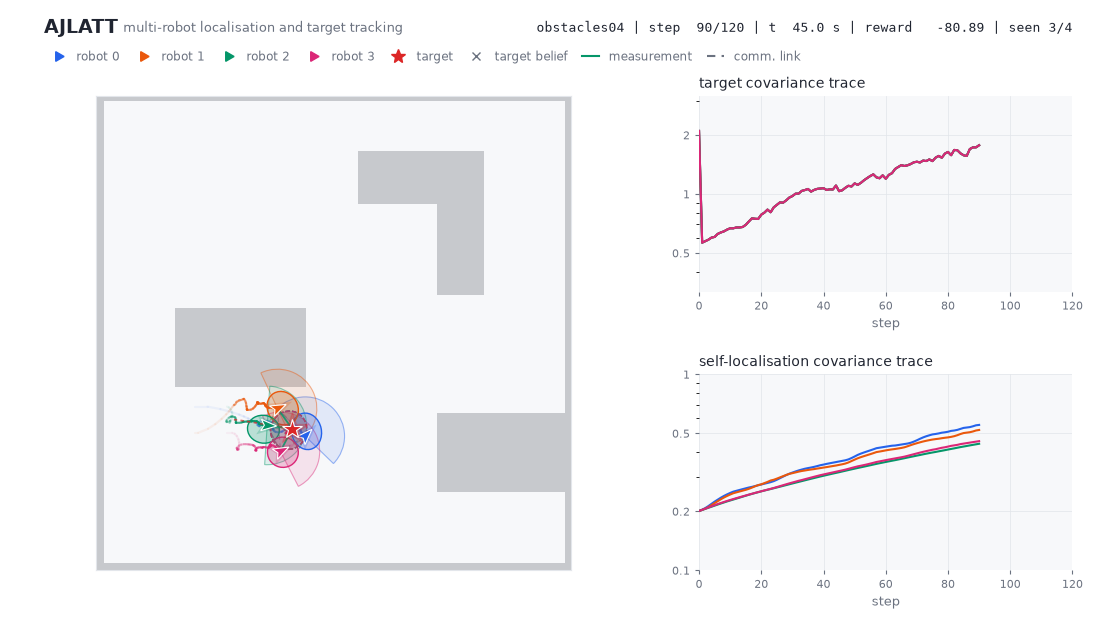
\includegraphics[width=\textwidth]{ajlatt.png}
  \caption{AJLATT dashboard on \code{obstacles04} (four robots running the
    encircling heuristic of the example script, step 90 of 120). The robots
    surround the target; the right panels show the trace of the target
    covariance and of the self-localisation covariances of the four robots.}
  \label{fig:ajlatt}
\end{figure}

% ---------------------------------------------------------------------------
\section{Registered id}\label{sec:ajlatt-ids}

\envid{AJLATT-v0} creates \code{AJLATTEnv} with the default configuration (four
robots on \code{obstacles04}). Gymnasium's passive environment checker is
disabled for this id because rewards and \code{terminated} are per-robot
arrays. Keyword arguments of \code{env\_lib.make} are configuration fields, for
example \code{env\_lib.make("AJLATT-v0", map\_name="obstacles05")}.

% ---------------------------------------------------------------------------
\section{Usage}\label{sec:ajlatt-usage}

The following controller sends robot $i$ to the $i$-th of $n_R$ evenly spaced
slots on a circle of radius 1.8\,m around its belief of the target, using only
the observation:

\begin{pycode}
import numpy as np
from env_lib import AJLATTEnv


def encircle(obs, layout, radius=1.8, gain=1.2):
    """Send robot i to the i-th slot of a circle around its target belief."""
    n = len(obs)
    pose = obs[:, layout["self_pose"]].astype(np.float64)   # x, y, theta
    rel = obs[:, layout["target_relative_position"]].astype(np.float64)
    c, s = np.cos(pose[:, 2]), np.sin(pose[:, 2])
    target = pose[:, :2] + np.column_stack([c * rel[:, 0] - s * rel[:, 1],
                                            s * rel[:, 0] + c * rel[:, 1]])
    angle = 2 * np.pi * np.arange(n) / n
    slot = target + radius * np.column_stack([np.cos(angle), np.sin(angle)])
    delta = slot - pose[:, :2]
    heading = np.arctan2(delta[:, 1], delta[:, 0])
    error = np.angle(np.exp(1j * (heading - pose[:, 2])))  # wrapped
    speed = np.minimum(2.0, 0.5 * np.linalg.norm(delta, axis=1))
    v = speed * np.maximum(0.0, np.cos(error))
    w = np.clip(gain * error, -np.pi / 4, np.pi / 4)
    return np.column_stack([v, w])


env = AJLATTEnv(map_name="obstacles04", num_robots=4)
layout = env.observation_layout()
obs, info = env.reset(seed=0)                  # obs: (4, 24) float32
episode_return = np.zeros(env.num_robots)
while True:
    obs, reward, terminated, truncated, info = env.step(encircle(obs, layout))
    episode_return += reward                   # per-robot rewards
    if truncated:                              # collision flags ignored
        break
stats = env.episode_statistics()               # arrays of shape (121, 4)
print(episode_return.sum(), info["episode_collisions"])
print(stats["target_cov_trace"][-1])
env.close()
\end{pycode}

The example script compares a similar heuristic with random actions and can
record an episode:

\begin{shellcode}
python examples/environments/ajlatt_demo.py --episodes 3
python examples/environments/ajlatt_demo.py --save renders/ajlatt.gif
python examples/environments/ajlatt_demo.py --map obstacles05 --render-mode human
\end{shellcode}

With the default configuration the heuristic of the script obtains a team
return of about $-7250$ per episode without collision events and keeps the
trace of the target covariance near 2, whereas random actions obtain returns of
$-25\,000$ or lower with dozens of collision events and target covariance traces
of 7 to 12 (the random actions are not seeded, so these values vary from run to
run).

% ---------------------------------------------------------------------------
\section{Reproducibility and performance}\label{sec:ajlatt-perf}

All randomness (initial beliefs, motion and measurement noise, the random target
policy and dynamic maps) is drawn from \code{self.np\_random}. If
\code{reset()} is called without a seed for the first time and
\code{config.seed} is set, that seed is used. With
\code{ci\_solver="slsqp"} trajectories match the implementation before
version 1.0 to about $10^{-6}$; the default Newton solver finds weights that
are at least as good and therefore produces slightly different, not worse,
estimates.

Measured on the development machine without rendering, a step takes 5--9\,ms on
\code{obstacles04} (90\,ms before 1.0) and 6--7\,ms on \code{obstacles05}
(67\,ms before). The gains come from exact batched Bresenham ray casting
(closest-obstacle queries are 7 to 19 times faster) and from the Newton
covariance-intersection solver. Rendering a frame takes about 25\,ms (about
110\,ms before). The cost of a step grows with the number of robots, because
every robot fuses the measurements and priors of its neighbours.

% ---------------------------------------------------------------------------
\section{Changes in 1.0}\label{sec:ajlatt-changes}

AJLATT was rewritten as a Gymnasium environment. See Appendix~\ref{app:migration}
for migration advice.

\begin{itemize}
  \item The environment class \code{AJLATTEnv} with its configuration
        dataclass \code{AJLATTConfig} replaces the former factory, which parsed
        the command line internally and therefore failed in scripts with their
        own command-line arguments. The legacy factory
        still works and translates the old names with a
        \code{DeprecationWarning}. Training options that used to live in the
        parameter module (PPO, LLM and debug settings) were removed; use
        \code{AJLATTConfig.add\_arguments}.
  \item \code{reset()} returns \code{(observation, info)}. Rendering is off by
        default; pass \code{render\_mode}.
  \item The spaces are joint multi-agent spaces with one row per robot, and
        rewards and \code{terminated} are per-robot arrays; the per-robot
        spaces are available as \code{single\_action\_space} and
        \code{single\_observation\_space}.
  \item The target-velocity entries of the observation contain the commanded
        target velocity instead of a configured constant.
  \item Fixed a memory leak: covariance traces accumulated across episodes
        (per-episode traces are now returned by \code{episode\_statistics()}).
        Also fixed: target policies were shared between environments and never
        reset, unknown maps triggered an interactive prompt, and dynamic maps
        did not work; they now resample at every reset and no longer need
        scikit-image. Three bundled maps that were one row short of their header
        were padded with a wall row.
  \item About ten times faster (Section~\ref{sec:ajlatt-perf}) and a new
        renderer.
  \item Map tools were consolidated into \code{env\_lib.ajlatt\_env.maps}; the
        builder now writes grids in the orientation the environment reads (the
        old builder produced transposed maps) and embeds its specification in
        the header.
  \item The id \envid{AJLATT-v1}, an unusable alias of \envid{AJLATT-v0}, was
        removed.
\end{itemize}

\endgroup

\chapter{Vectorised Simulation, Adapters, Baselines and Evaluation}\label{chap:workflow}

% Placeholder: written in the 1.1 update.


\part{Algorithms}
% ---------------------------------------------------------------------------
% Multi-agent reinforcement learning algorithms (marl_algorithms)
% ---------------------------------------------------------------------------
\begingroup
% Line breaking for paragraphs with long, unbreakable identifiers (local to
% this chapter): allow looser lines instead of overfull ones.
\setlength{\emergencystretch}{3em}\tolerance=1000
\chapter{Multi-Agent Reinforcement Learning Algorithms}\label{chap:marl}

The package \pkg{marl\_algorithms}, new in version 1.2, contains reference
implementations of seven classical algorithms for cooperative multi-agent
reinforcement learning: independent and multi-agent proximal policy
optimisation (IPPO, MAPPO), multi-agent deep deterministic policy gradient and
its twin-critic variant (MADDPG, MATD3), and independent Q-learning, value
decomposition networks and QMIX (IQL, VDN, QMIX). All seven are written
against one small core and train directly on the environments of
\pkg{env\_lib}: on the native batched vector environments where these exist,
with the per-agent rewards that every environment reports, and with evaluation
against the classical baseline controllers of
Section~\ref{sec:workflow-baselines}.

The code is meant to be read next to the papers. Every algorithm module cites
the method it implements, every class docstring states the loss it minimises,
and every simplification or deviation from the original method is stated in
the code and in this chapter. Tuned \emph{presets} train each algorithm on one
or more demonstration environments in at most about two minutes on a single
CPU core.
The package requires PyTorch (the \code{torch} extra,
Section~\ref{sec:install-extras}); \code{import marl\_algorithms} itself loads
nothing but the version number, and the first use of an algorithm imports
PyTorch.

% ---------------------------------------------------------------------------
\section{Overview}\label{sec:marl-overview}

Three parts of the package connect the algorithms to \pkg{env\_lib}:

\begin{enumerate}
  \item \emph{A per-agent view of the joint spaces.} The environments expose
    the whole team through joint spaces: observations stacked as
    \code{(n\_agents, obs\_dim)} and one joint action
    (Section~\ref{sec:envlib-joint}). \code{MultiAgentSpec} reads the number of
    agents, the size of one agent's observation and the kind and size of one
    agent's action from these spaces, and converts observations to per-agent
    arrays and per-agent actions back to the joint action
    (Section~\ref{sec:marl-spec}).
  \item \emph{Training on batched copies.} \code{make\_vector\_env} creates
    \code{num\_envs} copies of an environment with \code{env\_lib.make\_vec},
    which uses the native batched implementation when there is one
    (Section~\ref{sec:workflow-vector}), with the \code{"same\_step"}
    autoreset mode, so that every transition is a real one and the final
    observation of a truncated episode is available for bootstrapping. A
    \code{VectorRunner} turns every vector step into a \code{Transition} of
    per-agent arrays, including the per-agent rewards of
    \code{info["agent\_rewards"]} (Section~\ref{sec:marl-runner}).
  \item \emph{Evaluation with the \pkg{env\_lib} tools.} The method
    \code{policy()} of a trained algorithm returns a function from environment
    observations to environment actions that works for single and vector
    environments. The evaluation function \code{env\_lib.evaluate} therefore
    compares the trained policy with random actions and with the baseline
    controller on the same seeded episodes, and the recording function
    \code{record\_episode} of \pkg{env\_lib.utils} turns an episode of it
    into an animation (Section~\ref{sec:marl-quickstart}).
\end{enumerate}

Table~\ref{tab:marl-algorithms} lists the algorithms as registered in
\pkg{marl\_algorithms.registry}; the function \code{list\_algorithms()}
returns these records and the command \code{marl-train list} prints them.
Section~\ref{sec:marl-references} gives the full references cited in the
source code.

\begin{table}[htbp]
  \centering\small
  \caption{Registered algorithms. ``Family'' and ``Actions'' are the
    \code{family} and \code{action\_kinds} fields of \code{AlgorithmInfo}.}
  \label{tab:marl-algorithms}
  \begin{tabularx}{\textwidth}{@{}>{\raggedright\arraybackslash}p{1.35cm}>{\raggedright\arraybackslash}p{2.1cm}>{\raggedright\arraybackslash}p{1.8cm}>{\raggedright\arraybackslash}X>{\raggedright\arraybackslash}p{2.2cm}@{}}
    \toprule
    Name & Family & Actions & Key idea & Reference \\
    \midrule
    \code{ippo} & on-policy & continuous, discrete &
      PPO for every agent; decentralised critic $V(o_i)$ trained on the
      agent's own reward & de Witt et al.\ (2020) \\
    \code{mappo} & on-policy & continuous, discrete &
      decentralised PPO actors; centralised critic $V(s, i)$ on the global
      state, trained on the team reward & Yu et al.\ (2022) \\
    \code{maddpg} & off-policy actor-critic & continuous &
      deterministic actors $\mu_i(o_i)$; centralised critics
      $Q_i(s, a_1, \dots, a_n)$ on the global state and the joint action &
      Lowe et al.\ (2017) \\
    \code{matd3} & off-policy actor-critic & continuous &
      MADDPG with twin critics, target policy smoothing and delayed actor
      updates & Ackermann et al.\ (2019) \\
    \code{iql} & value-based & discrete &
      one DQN utility $Q_i(o_i, a_i)$ per agent, each trained on its own
      reward & Tan (1993) \\
    \code{vdn} & value-based & discrete &
      team value $\sum_i Q_i(o_i, a_i)$, trained end to end on the team
      reward & Sunehag et al.\ (2018) \\
    \code{qmix} & value-based & discrete &
      team value as a monotonic, state-conditioned mixture of the utilities
      (hypernetworks) & Rashid et al.\ (2018) \\
    \bottomrule
  \end{tabularx}
\end{table}

Every algorithm works on every environment whose action kind it supports.
Table~\ref{tab:marl-envs} shows the per-agent structure that
\code{MultiAgentSpec} reads from the registered environments; every
environment was trained briefly with an algorithm of each family that applies
to it, and an algorithm given an environment of the wrong action kind raises
\code{TypeError}.
Environments whose observation is not stacked per agent, the Kuramoto
environments, are treated as a single agent that observes and acts on the whole
network; with one agent IPPO and MAPPO reduce to PPO, MADDPG and MATD3 to DDPG
and TD3, and IQL to (double) DQN.

\begin{table}[htbp]
  \centering\small
  \caption{Per-agent structure of the registered environments as read by
    \code{MultiAgentSpec} (default parameters) and the algorithms that apply.
    $n$ is the number of agents and $d$ the size of one agent's observation.}
  \label{tab:marl-envs}
  \begin{tabularx}{\textwidth}{@{}>{\raggedright\arraybackslash}p{4.3cm}rr>{\raggedright\arraybackslash}p{3.1cm}>{\raggedright\arraybackslash}X@{}}
    \toprule
    Environment & $n$ & $d$ & Action per agent & Algorithms \\
    \midrule
    \envid{Consensus-v0}, \envid{Formation-v0} & 8 & 16 & continuous, 2-d & IPPO, MAPPO, MADDPG, MATD3 \\
    \envid{PowerGrid-v0} & 16 & 10 & continuous, 1-d & IPPO, MAPPO, MADDPG, MATD3 \\
    \envid{Platoon-v0} & 8 & 13 & continuous, 1-d & IPPO, MAPPO, MADDPG, MATD3 \\
    \envid{AJLATT-v0} & 4 & 24 & continuous, 2-d & IPPO, MAPPO, MADDPG, MATD3 \\
    \envid{Pistonball-v0} & 20 & 7 & continuous, 1-d; 3 choices with \code{continuous=False} & all seven, by action mode \\
    \envid{LineMsg-v0} (per-agent bits) & 10 & 3 & 2 choices & IPPO, MAPPO, IQL, VDN, QMIX \\
    \envid{WirelessComm-v1} (\envid{-v0}) & 16 (36) & 18 & 5 choices & IPPO, MAPPO, IQL, VDN, QMIX \\
    \envid{KuramotoOscillator-v0} (other Kuramoto ids: other sizes) & 1 & 75 & continuous, 55-d & IPPO, MAPPO, MADDPG, MATD3 \\
    \bottomrule
  \end{tabularx}
\end{table}

% ---------------------------------------------------------------------------
\section{Quick start}\label{sec:marl-quickstart}

\subsection{Training and evaluating from Python}

\code{marl\_algorithms.train} trains a registered algorithm on batched copies
of an environment and returns the trained algorithm together with its
\code{TrainingLog}. The run below is deliberately short (2\,000 environment
steps, a few seconds); the tuned MAPPO preset for \envid{PowerGrid-v0} trains
for 250\,000 steps (Section~\ref{sec:marl-results}).

\begin{pycode}
import env_lib
from marl_algorithms import train

# A short run; the tuned MAPPO preset for PowerGrid-v0 trains for 250_000 steps.
algo, log = train("mappo", "PowerGrid-v0", total_steps=2_000, num_envs=8,
                  seed=0)
print(algo)
print(len(log.episodes), "training episodes, mean return",
      round(log.mean_return(), 1))

envs = env_lib.make_vec("PowerGrid-v0", 16)
for name, policy in [("random", None), ("mappo", algo.policy()),
                     ("droop", env_lib.baseline_policy(envs))]:
    result = env_lib.evaluate(envs, policy, n_episodes=32, seed=1)
    print(f"{name:8s}{result.mean_return:10.2f}")
envs.close()
\end{pycode}

\begin{textcode}
MAPPO(16 agents, 10-d observations, continuous 1-d per agent, env_steps=2048)
8 training episodes, mean return -381.0
random     -613.22
mappo       -49.52
droop        -0.71
\end{textcode}

% norun
\begin{pycode}
train(algorithm, env_id, total_steps, *, num_envs=16, seed=0, env_kwargs=None,
      device="cpu", callback=None, **config) -> (Algorithm, TrainingLog)
\end{pycode}
creates the copies with \code{make\_vector\_env}, builds the algorithm with the
seed and the configuration overrides \code{**config} (field names of the
algorithm's configuration class; an unknown name raises \code{TypeError}),
trains it with \code{learn}, whose environment reset uses the same seed, and
closes the copies. On-policy algorithms stop after the first
complete rollout that reaches \code{total\_steps}, so the run above collected
2\,048 steps (two rollouts of 64 steps on 8 copies). The training returns in
the log are those of the exploratory policy; the evaluation uses the
deterministic policy (the mean action), which \code{algo.policy()} returns by
default.

The presets of Section~\ref{sec:marl-results} are looked up and trained with the
functions of \pkg{marl\_algorithms.presets}, which the top-level package also
exports:

\begin{pycode}
from marl_algorithms import get_preset, list_presets, train_preset

print(len(list_presets()), list_presets()[:2])
print(get_preset("qmix", "LineMsg-v0"))

# The preset trains for 25_000 steps; a smoke test overrides the length.
algo, log = train_preset("qmix", "LineMsg-v0", total_steps=2_000,
                         warmup_steps=500)
print(algo.config.lr, algo.config.batch_size, algo.env_steps)
\end{pycode}

\begin{textcode}
17 [('ippo', 'PowerGrid-v0'), ('ippo', 'Platoon-v0')]
{'num_envs': 16, 'total_steps': 25000, 'config': {'batch_size': 128,
'lr': 0.001, 'epsilon_decay_steps': 12500}, 'env_kwargs': {}}
0.001 128 2000
\end{textcode}

% norun
\begin{pycode}
train_preset(algorithm, env_id, *, seed=0, total_steps=None, num_envs=None,
             device="cpu", callback=None, **config) -> (Algorithm, TrainingLog)
\end{pycode}
calls \code{train} with the preset's values; \code{total\_steps},
\code{num\_envs} and configuration overrides replace them. It raises \code{KeyError} when the pair has no preset.
\code{get\_preset} returns a copy of the preset (or \code{None}), so it can be
modified freely.

A trained algorithm drives any environment of the same structure through
\code{policy()}, and \code{save} and \code{Algorithm.load} store and restore
it:

\begin{pycode}
import numpy as np
import env_lib
from env_lib.utils import record_episode
from marl_algorithms import Algorithm, make_vector_env, train

algo, log = train("vdn", "LineMsg-v0", total_steps=2_000, warmup_steps=500)

# Record the greedy policy on a single environment with per-agent actions.
env = env_lib.make("LineMsg-v0", action_space_type="multibinary",
                   render_mode="rgb_array")
frames = record_episode(env, algo.policy(), "renders/vdn_linemsg.gif",
                        seed=1, render_every=2)
env.close()

# Save and restore: the class and the configuration are read from the file.
path = algo.save("runs/vdn_linemsg.pt")
restored = Algorithm.load(path)
envs = make_vector_env("LineMsg-v0", 4)
obs = restored.spec.agent_obs(envs.reset(seed=0)[0])     # (4, 10, 3)
assert np.array_equal(restored.act(obs, deterministic=True),
                      algo.act(obs, deterministic=True))
print(type(restored).__name__, restored.env_steps, len(frames))
envs.close()
\end{pycode}

The file written by \code{save} holds the registry name, the
\code{MultiAgentSpec}, the configuration, the seed and the state (networks,
optimisers, counters and normalisation statistics); \code{Algorithm.load}
selects the class through the registry. The replay buffer of the off-policy
methods is not saved. Checkpoints are read with \code{torch.load(...,
weights\_only=False)} because they contain more than tensors, so load only
files from trusted sources.

\paragraph{Training in stages.} The method \code{learn} of an algorithm
(Section~\ref{sec:marl-base}) trains until the counter \code{algo.env\_steps}, which
persists across calls and through \code{save} and \code{load}, reaches
\code{total\_steps}; \code{total\_steps} is therefore a cumulative target, not
a number of additional steps. To continue a run, call \code{learn} again with
a larger total and pass the previous log to append to it. Every call resets
the copies with its \code{seed}, so episodes still running at the end of a
call are not completed. The callback is
called as \code{callback(algorithm, log)} after every update (on-policy) or
every round of gradient steps (off-policy); returning \code{False} stops
training. The environment copies passed to \code{learn} must use the
\code{"same\_step"} autoreset mode, which \code{make\_vector\_env} sets:

\begin{pycode}
from marl_algorithms import MATD3, make_vector_env

def stop_when_solved(algo, log):
    """Stop once the last 20 training episodes average more than -1600."""
    if log.mean_return(20) > -1600:     # NaN (no episode yet) compares False
        return False

envs = make_vector_env("Consensus-v0", 16)
algo = MATD3(envs, seed=0, reward_scale=0.01, normalize_observations=True)
log = algo.learn(envs, 3_200, seed=0)            # one episode per copy
log = algo.learn(envs, 6_400, seed=1, log=log,   # 3_200 more steps
                 callback=stop_when_solved)
print(algo.env_steps, algo.num_updates, len(log.episodes))
log.to_csv("runs/matd3_consensus.csv")
envs.close()
\end{pycode}

\subsection{The \texorpdfstring{\code{marl-train}}{marl-train} command line}\label{sec:marl-cli}

Installing the package provides the console script \code{marl-train}
(equivalently \code{python -m marl\_algorithms}) with the sub-commands of
Table~\ref{tab:marl-cli}. Values given with \code{-{}-set} and
\code{-{}-env-kwarg} are parsed as Python literals (plain text otherwise) and
override the preset's configuration and environment arguments.

\begin{table}[htbp]
  \centering\small
  \caption{Sub-commands of \code{marl-train} (defaults in brackets).}
  \label{tab:marl-cli}
  \begin{tabularx}{\textwidth}{@{}>{\raggedright\arraybackslash}p{0.36\textwidth}>{\raggedright\arraybackslash}X@{}}
    \toprule
    Command & Purpose \\
    \midrule
    \code{list} & the registered algorithms with family, action kinds, summary
      and reference \\
    \code{presets} & every \code{(algorithm, environment)} pair with a preset,
      with its steps and copies \\
    \code{run ALGORITHM ENV\_ID} & train (with the preset when there is one),
      print progress and a summary, optionally save the algorithm and the
      training episodes, then evaluate random actions, the trained policy and
      the baseline \\
    \quad \code{-{}-steps N}, \code{-{}-num-envs N} & environment steps and
      batched copies [preset; 100\,000 and 16 without a preset] \\
    \quad \code{-{}-seed S} & seed of training [0]; the evaluation uses
      \code{S + 1} \\
    \quad \code{-{}-no-preset} & ignore the preset and use the defaults of the
      configuration class \\
    \quad \code{-{}-set KEY=VALUE ...} & configuration overrides \\
    \quad \code{-{}-env-kwarg KEY=VALUE ...} & environment arguments \\
    \quad \code{-{}-eval-episodes N} & evaluation episodes [64]; 0 skips the
      evaluation \\
    \quad \code{-{}-reports N} & progress lines during training [10] \\
    \quad \code{-{}-save PATH}, \code{-{}-csv PATH} & save the algorithm
      (\code{Algorithm.save}) and the training episodes
      (\code{TrainingLog.to\_csv}) \\
    \quad \code{-{}-threads N} & PyTorch threads [1]; 0 keeps the PyTorch
      default \\
    \code{compare ENV\_ID} & train baseline algorithms over one or more
      seeds and compare them with random actions and the classical controller
      on the same episodes (Section~\ref{sec:marl-baselines}) \\
    \quad \code{-{}-algos ALGO ...} & algorithms [every one with a preset for
      the environment] \\
    \quad \code{-{}-seeds S ...} & training seeds [0] \\
    \quad \code{-{}-steps N}, \code{-{}-num-envs N} & budget and copies per run
      [preset] \\
    \quad \code{-{}-episodes N}, \code{-{}-eval-seed S} & evaluation episodes
      [64] and seed [1] \\
    \quad \code{-{}-set}, \code{-{}-env-kwarg} & as for \code{run} \\
    \quad \code{-{}-markdown}, \code{-{}-csv PATH} & print a Markdown table,
      save the report as CSV \\
    \quad \code{-{}-save-dir DIR} & save every trained algorithm as
      \code{DIR/NAME\_seedS.pt} \\
    \code{evaluate CHECKPOINT ENV\_ID} & evaluate a saved algorithm against
      random actions and the baseline \\
    \quad \code{-{}-episodes N}, \code{-{}-seed S} & evaluation episodes [64]
      and seed [1] \\
    \quad \code{-{}-env-kwarg KEY=VALUE ...} & environment arguments (as used
      in training) \\
    \bottomrule
  \end{tabularx}
\end{table}

\begin{shellcode}
marl-train list                       # algorithms and references
marl-train presets                    # tuned (algorithm, environment) pairs
marl-train run mappo PowerGrid-v0     # train with the preset, then evaluate
marl-train run qmix LineMsg-v0 --steps 50000 --set lr=1e-3
marl-train run maddpg Consensus-v0 --save runs/maddpg.pt --csv runs/maddpg.csv
marl-train evaluate runs/maddpg.pt Consensus-v0 --episodes 64
marl-train run ippo Formation-v0 --no-preset --steps 200000 --num-envs 32 \
    --set lr=1e-3 normalize_observations=False --env-kwarg formation_shape=wedge
\end{shellcode}

The evaluation of \code{run} and \code{evaluate} uses
\code{make\_vector\_env(env\_id, min(episodes, 64))}, so up to 64 episodes run in
parallel. Output of \code{marl-train run qmix LineMsg-v0} (the complete preset;
wall-clock times depend on the machine):

\begin{textcode}
Training qmix on LineMsg-v0 (preset): 25,000 env steps, 16 copies, seed 0
       2,512 steps  mean return (last 20)        43.02     2.7 s
       5,008 steps  mean return (last 20)        54.33     4.7 s
       ...
      22,512 steps  mean return (last 20)        92.35    17.3 s
      25,008 steps  mean return (last 20)        91.96    19.1 s
qmix on LineMsg-v0: 496 episodes, 25008 env steps, mean return (last 100) 92.18, 17.0 s

Evaluation on LineMsg-v0, 64 episodes (seed 1):
  policy       mean return   95% CI +-   length
  random              43.2        1.17     50.0
  qmix                  95           0     50.0
  baseline              95           0     50.0
\end{textcode}

The progress lines report the mean return of the last 20 exploratory training
episodes; the summary line is \code{TrainingLog.summary()}, whose step count
and time refer to the last record of the log (an update or a finished
episode). The evaluation columns
are the mean team return of the deterministic policy, the half-width of its
95\,\% confidence interval and the mean episode length
(Table~\ref{tab:workflow-result}).

% ---------------------------------------------------------------------------
\section{Using the algorithms as baselines}\label{sec:marl-baselines}

A new method for one of the environments is judged against established ones.
Three kinds of reference are available for every environment: uniformly
random actions (the floor), the environment's classical controller
(\code{env\_lib.baseline\_policy}, the standard of its field) and the seven
learning algorithms, with tuned presets for the environments of
Table~\ref{tab:marl-presets}. The function \code{marl\_algorithms.compare}
trains the learning baselines, over as many seeds as you ask for, and
evaluates everything, your methods included, on the same seeded episodes.

\subsection{In one call}

\begin{pycode}
import numpy as np
from marl_algorithms import compare

def my_policy(obs):
    """Your method: (num_envs, n_agents, obs_dim) -> (num_envs, n_agents)."""
    return np.zeros(obs.shape[:-1], dtype=np.float32)   # replace me

report = compare("PowerGrid-v0", ["mappo", "ippo"], seeds=(0, 1),
                 policies={"my method": my_policy},
                 total_steps=4_096, num_envs=16)       # small budget: seconds
print(report)
report.to_csv("runs/power_grid_comparison.csv")
\end{pycode}

Without \code{total\_steps} and \code{num\_envs} every algorithm trains with
its preset. The script \code{examples/algorithms/baseline\_comparison.py} runs
exactly this comparison with a proposed method, a distributed droop controller
that also reacts to the neighbours' mean frequency deviation, and the full
presets (about six minutes on one core):

\begin{textcode}
PowerGrid-v0: mean team return over 64 evaluation episodes (seed 1); higher is better

method     kind       mean return    std  seeds  env steps  train [s]
---------  ---------  -----------  -----  -----  ---------  ---------
random     reference       -629.3      -      -          -          -
baseline   reference       -0.786      -      -          -          -
mappo      algorithm        -1.02  0.182      2    251,904      101.9
ippo       algorithm        -2.25  0.172      2    200,704       65.2
my method  policy          -0.675      -      -          -          -
\end{textcode}


\begin{figure}[htbp]
  \centering
  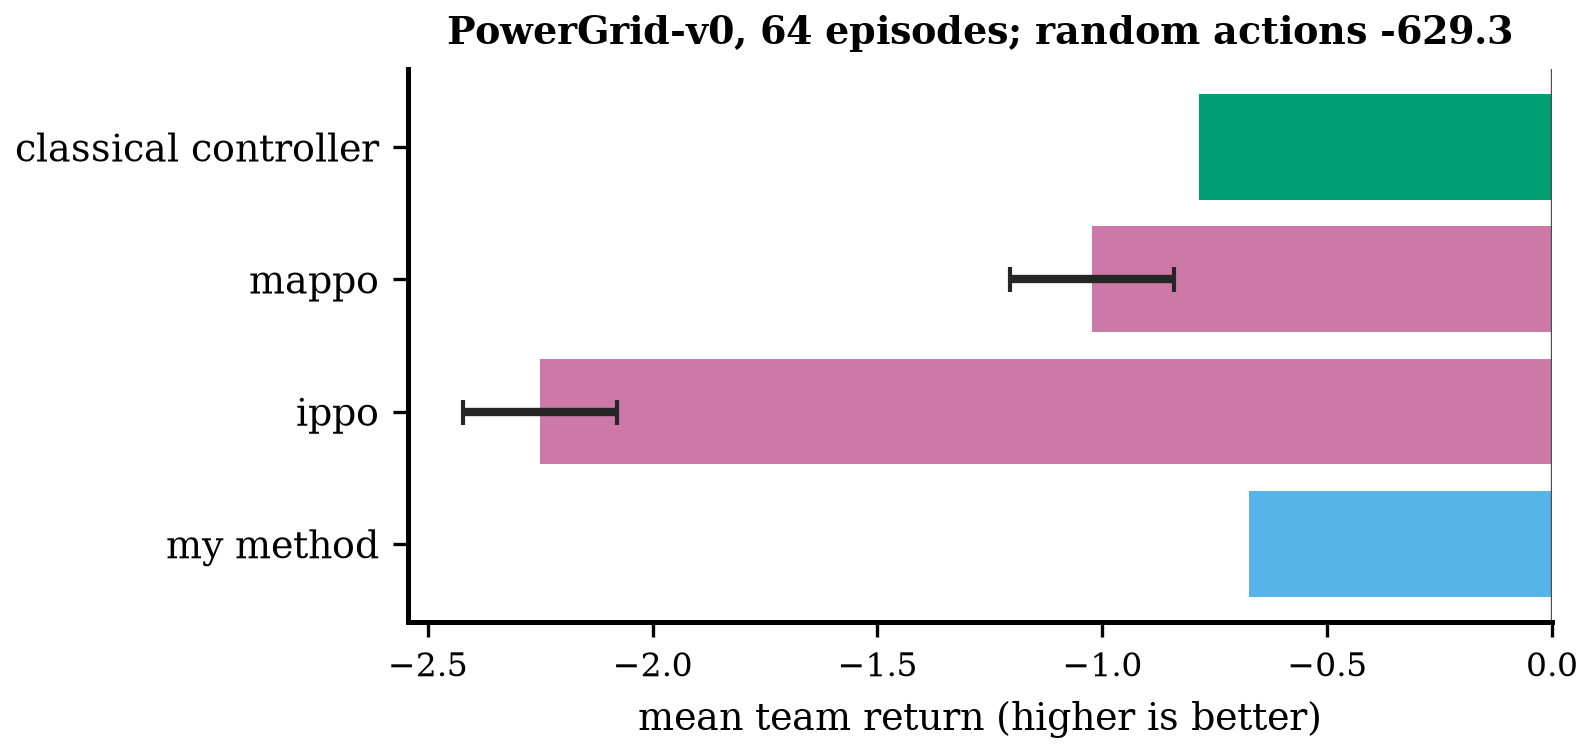
\includegraphics[width=0.72\textwidth]{baseline_comparison.png}
  \caption{Output figure of \code{baseline\_comparison.py}: mean return on
    \envid{PowerGrid-v0} over 64 evaluation episodes; the error bars are the
    standard deviation over two training seeds. Random actions ($-629.3$) are
    off the scale.}
  \label{fig:marl-baselines}
\end{figure}

Figure~\ref{fig:marl-baselines} draws the same numbers. The rows are the
references first, then the algorithms with the mean and the
standard deviation over the training seeds, the environment steps and the
wall-clock training time of one run, then your policies. \code{compare} works
in four steps:

\begin{enumerate}
  \item it creates the evaluation environment,
    \code{make\_vector\_env(env\_id, min(n\_episodes, 64), **env\_kwargs)};
  \item it evaluates random actions, the classical controller (when the
    environment has one) and your policies, first, so that an error in a
    policy shows before any training;
  \item it trains every algorithm once per seed, with its preset
    (\code{train\_preset}) or, without a preset, with its default
    configuration and \code{total\_steps}, and evaluates the deterministic
    policy;
  \item it returns a \code{Comparison}, which also keeps every trained
    algorithm and training log.
\end{enumerate}

Every evaluation resets the same environment copies with the same seed, so all
rows see identical initial conditions and disturbances. With the default
training seed 0 and evaluation seed 1 the numbers reproduce the published
results of Table~\ref{tab:marl-results-table}.

\subsection{From the command line}

\begin{shellcode}
marl-train compare PowerGrid-v0                       # every preset algorithm, seed 0
marl-train compare PowerGrid-v0 --algos mappo ippo --seeds 0 1 2 --csv runs/pg.csv
marl-train compare LineMsg-v0 --markdown              # a table for a README or a paper
marl-train compare Consensus-v0 --save-dir runs/baselines  # keep the trained baselines
marl-train compare Formation-v0 --algos mappo --steps 200000   # no preset: set a budget
\end{shellcode}

\code{marl-train compare} checks the environment, the algorithm names, their
action kinds and the \code{-{}-set} fields before training
(Table~\ref{tab:marl-cli}).

\subsection{Recipes}

\begin{description}[leftmargin=0.6cm,style=nextline]
  \item[Choose the baselines and the budget]
    \code{algorithms=["mappo", "maddpg"]} selects methods (by default every
    algorithm with a preset for the environment, \code{marl-train presets});
    \code{seeds=(0, 1, 2, 3, 4)} adds seeds; \code{total\_steps} and
    \code{num\_envs} replace the presets' budget, for example for a quick
    check before a long run.
  \item[Another configuration of the environment]
    \code{env\_kwargs=\{"n\_buses": 32\}} trains and evaluates every method on
    the variant. The presets' hyperparameters are kept; a larger variant may
    need a larger \code{total\_steps}.
  \item[An algorithm without a preset]
    Pass \code{total\_steps} to train it with its default configuration, or
    tune it yourself with \code{train(...)} and pass the trained algorithm in
    \code{policies}.
  \item[A policy written for a single environment]
    \code{compare} evaluates batched observations. Wrap a policy that maps one
    observation \code{(n\_agents, obs\_dim)} to one action with
    \code{per\_copy(policy)}; batched policies are faster.
  \item[A method built on this package]
    A modified algorithm (a new loss, another critic) is an \code{Algorithm}:
    train it and pass the object in \code{policies}; its deterministic policy
    is evaluated like the baselines. For several seeds of your method, train
    one per seed and pass them under separate names, or register it
    (Section~\ref{sec:marl-extending}) and list it in \code{algorithms}.
  \item[Reuse the trained baselines]
    \code{report.algorithms[("mappo", 0)]} is the trained MAPPO of seed 0:
    save it, record an episode with \code{record\_episode(env,
    algo.policy(), path)} or evaluate it on other scenarios;
    \code{report.logs} holds the training logs for learning curves
    (Section~\ref{sec:plotkit-curves}).
  \item[Tables and further analysis]
    \code{report.to\_markdown()}, \code{report.to\_csv(path)} and
    \code{report.records()} (one dictionary per row, for example for
    \code{pandas.DataFrame}); \code{report["mappo"].returns} gives the
    per-seed returns and \code{report.ranking()} orders the algorithms and
    your policies by mean return.
\end{description}

% ---------------------------------------------------------------------------
\section{Design of the core}\label{sec:marl-core}

The package separates what all methods share, what distinguishes each
method, and the settings tuned for the environments. Every algorithm has its
own module, next to the \code{common} module of its family, and the algorithm
modules contain only what is specific to them:

\begin{textcode}
src/marl_algorithms/
  __init__.py           lazy exports (train, compare, algorithms, ...)
  __main__.py           the marl-train command line
  registry.py           AlgorithmInfo, get_algorithm, make_algorithm, train
  baselines.py          compare, Comparison, per_copy: baselines
  core/                 shared by all methods
    spec.py             MultiAgentSpec: per-agent view of the joint spaces
    runner.py           make_vector_env, VectorRunner, Transition
    buffers.py          RolloutBuffer, compute_gae, ReplayBuffer
    normalization.py    RunningMeanStd, ObservationNormalizer, RewardScaler
    networks.py         mlp, policies, QMixer, PerAgent, agent_one_hot,
                        soft_update
    config.py           AlgorithmConfig, OnPolicyConfig, OffPolicyConfig
    base.py             Algorithm, OnPolicyAlgorithm, OffPolicyAlgorithm,
                        TrainingLog
  algorithms/           one module per algorithm, grouped by family
    ppo/                on-policy
      common.py         PPOConfig and the shared PPO implementation
      ippo.py           IPPO (decentralised critics)
      mappo.py          MAPPO (centralised critic)
    ddpg/               off-policy actor-critic
      common.py         DDPGConfig and the shared implementation
      maddpg.py         MADDPG
      matd3.py          MATD3 (twin critics, smoothing, delayed actors)
    q_learning/         value-based
      common.py         QLearningConfig and the shared implementation
      iql.py            IQL (no mixing)
      vdn.py            VDN and VDNMixer (additive mixing)
      qmix.py           QMIX (monotonic mixing with QMixer)
  presets/              tuned settings for the env_lib environments
    __init__.py         PRESETS, get_preset, list_presets, train_preset
    ppo.py, ddpg.py, q_learning.py
                        the tables of each family, with tuning notes
\end{textcode}

The docstring of every family package (for example
\code{help(marl\_algorithms.algorithms.ppo)}) describes the methods, the
implementation choices and the references; the docstring of every class gives
its losses.

\subsection{The per-agent view: \texorpdfstring{\code{MultiAgentSpec}}{MultiAgentSpec}}\label{sec:marl-spec}

\code{MultiAgentSpec.from\_env(env)} reads the agent structure of a single or
vector environment (from \code{single\_observation\_space} and
\code{single\_action\_space} when present) and
\code{MultiAgentSpec.from\_spaces(observation\_space, action\_space)} from the
spaces. The spec is a frozen dataclass with the fields \code{n\_agents},
\code{obs\_dim}, \code{action\_kind} (\code{"continuous"} or
\code{"discrete"}), \code{action\_dim} (1 for discrete actions),
\code{n\_actions} (discrete only), \code{action\_low} and \code{action\_high}
(continuous only, shape \code{(n\_agents, action\_dim)}), \code{obs\_shape},
\code{action\_shape} and \code{action\_dtype}. The observation space must be a
\code{Box}; the action spaces are read as follows.

\begin{itemize}
  \item \code{Box} of shape \code{(n, d)} with observations \code{(n, obs\_dim)}:
    $n$ agents with $d$-dimensional continuous actions; shape \code{(n,)}: $n$
    agents with one action each. Any other \code{Box} is a single agent whose
    action is the flattened box (the Kuramoto environments). The bounds must be
    finite; they may differ between agents and dimensions.
  \item \code{MultiDiscrete} and \code{MultiBinary}: one agent per entry, with
    the same number of choices for every agent; \code{MultiDiscrete} must
    start at 0.
  \item \code{Discrete}: only for a single agent. A joint \code{Discrete}
    action over several agents, such as the default \code{Discrete(2 ** n)}
    action of LineMsg, raises \code{TypeError}; \code{make\_vector\_env}
    therefore creates LineMsg with \code{action\_space\_type="multibinary"}.
  \item With several agents the observation must be stacked as
    \code{(n, obs\_dim)}; with one agent it is flattened.
\end{itemize}

\code{spec.agent\_obs(obs)} returns observations with any leading batch shape
as \code{float32} arrays \code{(*batch, n\_agents, obs\_dim)};
\code{spec.env\_action(actions)} converts per-agent actions,
\code{(*batch, n\_agents, action\_dim)} floats (or \code{(*batch, n\_agents)}
when \code{action\_dim} is 1) or \code{(*batch, n\_agents)} integers, into the
joint action and clips continuous actions to the bounds. The property
\code{state\_dim} $= n \cdot \code{obs\_dim}$ is the size of the global state
$s = [o_1, \dots, o_n]$ that the centralised critics and the QMIX mixer use:
none of the environments exposes a separate state, so the global state is the
concatenation of all agents' observations. \code{describe()} returns a one-line
summary such as \code{"16 agents, 10-d observations, continuous 1-d per agent"}.

\subsection{Collecting experience: \texorpdfstring{\code{VectorRunner}}{VectorRunner} and \texorpdfstring{\code{Transition}}{Transition}}\label{sec:marl-runner}

% norun
\begin{pycode}
make_vector_env(env_id, num_envs=16, **env_kwargs)
# = env_lib.make_vec(env_id, num_envs, autoreset_mode="same_step", **env_kwargs)
\end{pycode}
creates the training copies; for LineMsg it sets
\code{action\_space\_type="multibinary"} unless the argument is given. Environments without a native vector implementation (LineMsg,
WirelessComm, Pistonball, AJLATT and the PyTorch Kuramoto ids) are simulated
with Gymnasium's \code{SyncVectorEnv}.

\code{VectorRunner(envs, spec=None)} steps such a vector environment in
per-agent form; it raises \code{ValueError} for any autoreset mode other than
\code{"same\_step"}. \code{reset(seed=None)} resets all copies and returns
observations \code{(B, n, obs\_dim)}; \code{step(actions)} applies per-agent
actions to all copies and returns a \code{Transition}
(Table~\ref{tab:marl-transition}), after which \code{runner.obs} holds the
observations to act on next; \code{pop\_episodes()} returns and clears the
\code{(return, length)} pairs of the episodes finished so far.

\begin{table}[htbp]
  \centering\small
  \caption{Fields of \code{Transition} ($B$ copies, $n$ agents).}
  \label{tab:marl-transition}
  \begin{tabularx}{\textwidth}{@{}>{\raggedright\arraybackslash}p{3.3cm}>{\raggedright\arraybackslash}p{3.4cm}>{\raggedright\arraybackslash}X@{}}
    \toprule
    Field & Shape & Content \\
    \midrule
    \code{obs} & \code{(B, n, obs\_dim)} & observations the actions were taken in \\
    \code{actions} & \code{(B, n, action\_dim)} or \code{(B, n)} & per-agent actions as passed to \code{step} (unclipped) \\
    \code{reward} & \code{(B,)} & team rewards \\
    \code{agent\_rewards} & \code{(B, n)} & per-agent rewards from \code{info["agent\_rewards"]}; the team reward for every agent when the environment reports none \\
    \code{next\_obs} & \code{(B, n, obs\_dim)} & successor observations; the \emph{final} observation for copies whose episode ended \\
    \code{terminated}, \code{truncated} & \code{(B,)} & episode-end flags; the property \code{done} is their disjunction \\
    \bottomrule
  \end{tabularx}
\end{table}

With same-step autoreset a finished copy is reset within the step, so the
observation returned by the environment already belongs to the next episode.
The runner therefore takes the final observation from
\code{infos["final\_obs"]} and the final per-agent rewards from
\code{infos["final\_info"]["agent\_rewards"]}. Every transition is a real one
(there is no reset step to skip, as with next-step autoreset), and the value
of the final observation is available to bootstrap episodes that were
truncated by the time limit. Only \code{terminated} stops the bootstrap in the
algorithms; \code{truncated} only cuts the advantage recursion.

\subsection{Buffers and generalised advantage estimation}\label{sec:marl-buffers}

\paragraph{Rollouts.} \code{RolloutBuffer(length, num\_envs, fields)} stores
named arrays of shape \code{(T, B, ...)}, with \code{fields} a dictionary
\code{\{name: (trailing\_shape, dtype)\}}. \code{add(**values)} stores one
vector step (every field must be given), \code{buffer[name]} returns the
stored steps, \code{full} tells whether $T$ steps are stored and
\code{reset()} starts a new rollout in the same arrays.

\paragraph{GAE.} The function

% norun
\begin{pycode}
compute_gae(rewards, values, next_values, terminated, truncated, gamma,
            gae_lambda) -> (advantages, returns)
\end{pycode}
works on arrays of shape \code{(T, B, ...)}; trailing dimensions such as
agents are broadcast against the \code{(T, B)} flags. With $V_t = V(o_t)$,
$V'_t$ the value of the successor observation $o'_t$ (the final observation
when the episode ended), $\tau_t$ the \code{terminated} flag of step $t$ and
$\mathrm{done}_t$ the flag that is set when the episode terminated or was
truncated at step $t$,
\begin{align}
  \delta_t &= r_t + \gamma\,(1 - \tau_t)\, V'_t - V_t, \label{eq:marl-td}\\
  A_t &= \delta_t + \gamma \lambda\, (1 - \mathrm{done}_t)\, A_{t+1},
  \qquad A_T = 0, \label{eq:marl-gae}\\
  R_t &= A_t + V_t. \nonumber
\end{align}
The recursion runs backwards from the last step of the rollout, where the
bootstrap enters through $V'_{T-1}$ in $\delta_{T-1}$. A terminated episode
does not bootstrap, a truncated one bootstraps from the value of its final
observation, and neither passes advantages across the episode boundary. A test
compares the function with this recursion written out step by step.

\paragraph{Replay.} \code{ReplayBuffer(capacity, spec)} is a circular buffer of
joint transitions. Its method \code{add(transition)} stores every copy of a
vector transition, one entry per copy and step, so the capacity counts
transitions rather than vector steps. The method \code{sample(batch\_size,
rng)} draws transitions uniformly with replacement using the algorithm's
generator and returns a dictionary of NumPy arrays:

\begin{textcode}
obs, next_obs      (N, n, obs_dim)       float32
actions            (N, n, action_dim)    float32   (continuous actions)
                   (N, n)                int64     (discrete actions)
reward             (N,)                  float32
agent_rewards      (N, n)                float32
terminated         (N,)                  float32
\end{textcode}

Truncation is not stored, because the stored successor of a truncated
transition is its final observation and the target bootstraps from it.

\subsection{Normalisation}\label{sec:marl-normalisation}

\code{RunningMeanStd(shape=())} keeps a running mean $\mu$, variance
$\sigma^2$ and count $N$ (initially $10^{-4}$) and includes a batch with mean
$\mu_b$, variance $\sigma_b^2$ and size $N_b$ with the parallel update rule
\begin{equation}
  \Delta = \mu_b - \mu, \quad
  \mu \leftarrow \mu + \Delta \frac{N_b}{N + N_b}, \quad
  \sigma^2 \leftarrow \frac{N \sigma^2 + N_b \sigma_b^2
      + \Delta^2 N N_b / (N + N_b)}{N + N_b}, \quad
  N \leftarrow N + N_b .
\end{equation}

\code{ObservationNormalizer(obs\_dim, clip=10.0, enabled=True)} standardises
observations feature by feature, $\hat o = \operatorname{clip}((o - \mu) /
\sigma, -10, 10)$, with statistics \emph{shared by all agents}: every agent's
observation of every copy is a sample of the same per-feature statistics, as
befits homogeneous agents with shared parameters. \code{update(obs)} adds
observations of any leading shape; with \code{enabled=False} the normaliser
returns its input unchanged.

\code{RewardScaler(num\_envs, gamma, enabled=True)} divides rewards by the
running standard deviation of the discounted return. Every copy $b$ keeps a
return $G_b \leftarrow \gamma G_b + \bar r_b$, where $\bar r_b$ is the reward of
copy $b$ averaged over its trailing dimensions (the agents), the statistics
include the new $G_b$, the returns of finished copies are reset to zero, and
the rewards are returned as $r / \sigma_G$. Rewards are scaled, not centred, so
the optimal policy is unchanged, while value targets become of order one
whether an environment's rewards are of order $10^{-3}$ per step (PowerGrid)
or $10^{2}$ (Consensus).

\subsection{Networks}\label{sec:marl-networks}

The building blocks of \pkg{marl\_algorithms.core.networks} take per-agent
inputs with arbitrary leading dimensions \code{(..., features)}:

% norun
\begin{pycode}
mlp(in_dim, out_dim, hidden_sizes=(64, 64), activation="tanh", *,
    output_gain=1.0, layer_norm=False)
PerAgent(factory, n_agents, shared=True)
GaussianPolicy(in_dim, action_dim, low, high, hidden_sizes, activation,
               log_std_init=-0.5)
CategoricalPolicy(in_dim, n_actions, hidden_sizes, activation)
DeterministicPolicy(in_dim, action_dim, low, high, hidden_sizes,
                    activation="relu")
QMixer(n_agents, state_dim, embed_dim=32, hypernet_hidden=64)
agent_one_hot(batch_shape, n_agents, device)
soft_update(target, source, tau)
\end{pycode}

\begin{itemize}
  \item \code{mlp} builds a multi-layer perceptron with orthogonal
    initialisation (gain $\sqrt{2}$ for ReLU-type activations, $5/3$ for
    tanh) and zero biases; the activation is \code{"tanh"}, \code{"relu"},
    \code{"elu"} or \code{"gelu"}. The policy heads use
    \code{output\_gain=0.01}, which makes the initial policies nearly uniform
    (categorical) or centred in the action range (Gaussian, deterministic).
  \item \code{PerAgent} with \code{shared=True} applies one network, built by
    \code{factory()}, to all agents in one call; with \code{shared=False}
    every agent has its own network and agent $i$'s slice of the input goes
    through network $i$. \code{call(method, x, *args)} dispatches any method
    of the underlying networks in the same way (tensor arguments are sliced
    per agent, others, such as a \code{torch.Generator}, are passed
    unchanged).
  \item Agent identifiers: when parameters are shared and
    \code{agent\_ids=True} (both defaults) and there is more than one agent,
    the one-hot identifier $e_i \in \{0, 1\}^n$ of agent $i$ is appended to
    its input, $x_i = [\hat o_i, e_i]$, so that agents sharing one network can
    still behave differently. \code{Algorithm.agent\_inputs(obs)} builds these
    inputs for all agents at once with \code{agent\_one\_hot}.
  \item \code{GaussianPolicy} is a diagonal Gaussian with a state-independent
    standard deviation, expressed in units of the action range: with the
    centre $c = (\text{high} + \text{low})/2$ and the half-range
    $h = (\text{high} - \text{low})/2$,
    $\pi_\theta(\cdot \mid x) = \mathcal{N}\bigl(c + h \odot f_\theta(x),\;
    \operatorname{diag}(h \odot e^{\ell})^2\bigr)$ with the learned vector
    $\ell$ initialised to \code{log\_std\_init}. Samples are unbounded; the
    log-density $\sum_k \log \mathcal{N}(a_k)$ is that of the unclipped sample,
    and the entropy is $\sum_k \bigl(\tfrac12 + \tfrac12 \log 2\pi + \log
    \sigma_k\bigr)$. A shared policy keeps the bounds of all agents, so agents
    with different action ranges can share it.
  \item \code{CategoricalPolicy} returns the logits of a categorical
    distribution; like \code{GaussianPolicy} it provides
    \code{sample(x, generator)} (actions and log-probabilities) and
    \code{log\_prob(x, action)} (log-probabilities and entropy).
  \item \code{DeterministicPolicy} computes $\mu_\theta(x) = c + h \odot
    \tanh f_\theta(x)$, always within the bounds.
  \item \code{QMixer} is the monotonic mixing network of QMIX
    (Section~\ref{sec:marl-value}), and \code{soft\_update} performs Polyak
    averaging, $\theta' \leftarrow (1 - \tau)\theta' + \tau\theta$.
\end{itemize}

\subsection{Base classes and training loops}\label{sec:marl-base}

Every algorithm derives from \code{Algorithm}:

% norun
\begin{pycode}
Algorithm(spec, config=None, *, device="cpu", seed=None, **overrides)
\end{pycode}

\code{spec} is a \code{MultiAgentSpec} or an environment (single or vector) to
read it from; \code{config} an instance of the class attribute
\code{config\_class} (defaults to \code{config\_class()}); \code{overrides}
replace configuration fields with \code{dataclasses.replace}. An environment
whose action kind is not in the class attribute \code{action\_kinds}, a
configuration of the wrong class and an unknown field raise \code{TypeError};
invalid values raise \code{ValueError} when the configuration is created.
Table~\ref{tab:marl-config-common} lists the fields shared by all algorithms.

\begin{table}[htbp]
  \centering\small
  \caption{Configuration fields shared by the algorithms
    (\pkg{marl\_algorithms.core.config}). \code{PPOConfig} derives from
    \code{OnPolicyConfig}, \code{DDPGConfig} and \code{QLearningConfig} from
    \code{OffPolicyConfig}; both derive from \code{AlgorithmConfig}.}
  \label{tab:marl-config-common}
  \begin{tabularx}{\textwidth}{@{}>{\raggedright\arraybackslash}p{4.3cm}>{\raggedright\arraybackslash}p{1.8cm}>{\raggedright\arraybackslash}X@{}}
    \toprule
    Field & Default & Meaning \\
    \midrule
    \multicolumn{3}{@{}l}{\emph{\code{AlgorithmConfig} (all algorithms)}} \\
    \code{hidden\_sizes} & \code{(64, 64)} & widths of the hidden layers of every network \\
    \code{activation} & \code{"tanh"} & hidden activation (\code{"tanh"}, \code{"relu"}, \code{"elu"}, \code{"gelu"}) \\
    \code{gamma} & 0.99 & discount factor $\gamma$ \\
    \code{share\_parameters} & \code{True} & one set of network weights for all agents \\
    \code{agent\_ids} & \code{True} & append one-hot agent identifiers to per-agent inputs when parameters are shared \\
    \code{max\_grad\_norm} & 10.0 & gradient-norm clipping threshold \\
    \midrule
    \multicolumn{3}{@{}l}{\emph{\code{OnPolicyConfig} (IPPO, MAPPO)}} \\
    \code{max\_grad\_norm} & 0.5 & overrides the default above \\
    \code{rollout\_length} & 64 & vector steps $T$ per rollout ($T \cdot B$ transitions per update) \\
    \code{lr} & $3 \cdot 10^{-4}$ & Adam learning rate (of the actor for PPO) \\
    \code{gae\_lambda} & 0.95 & GAE parameter $\lambda$ \\
    \code{normalize\_observations} & \code{True} & standardise observations with running statistics \\
    \code{normalize\_rewards} & \code{True} & scale rewards by the running standard deviation of the return \\
    \midrule
    \multicolumn{3}{@{}l}{\emph{\code{OffPolicyConfig} (MADDPG, MATD3, IQL, VDN, QMIX)}} \\
    \code{activation} & \code{"relu"} & overrides the default above \\
    \code{buffer\_size} & 200\,000 & replay capacity in transitions (one per copy and step) \\
    \code{batch\_size} & 256 & transitions per gradient step \\
    \code{warmup\_steps} & 2\,000 & environment steps (summed over copies) with uniformly random actions before learning starts \\
    \code{update\_every} & 1 & vector steps between rounds of gradient steps \\
    \code{gradient\_steps} & 1 & gradient steps per round \\
    \code{tau} & 0.01 & Polyak coefficient $\tau$ of the target networks \\
    \code{reward\_scale} & 1.0 & constant factor $\kappa$ applied to rewards before learning \\
    \bottomrule
  \end{tabularx}
\end{table}

\paragraph{Seeding without global side effects.} The seed initialises a
\code{numpy.random.SeedSequence}, from which the algorithm derives its own
NumPy generator \code{self.np\_rng} (random warm-up actions, replay sampling,
$\epsilon$-greedy draws) and a seed for its own \code{torch.Generator}
\code{self.torch\_rng} (policy samples, exploration and target-smoothing noise,
minibatch permutations). The networks are built inside
\code{torch.random.fork\_rng}, seeded from the same sequence, so network
initialisation is reproducible while PyTorch's global random state is restored
afterwards. Apart from this temporary, forked seeding, no code of the package
seeds or draws from the global NumPy or PyTorch generators, and none changes
the number of PyTorch threads; the scripts and \code{marl-train} set the
thread count themselves. With the same seed and the same machine, training is identical
(the tests check this for every algorithm); \code{seed=None} draws fresh
entropy.

\paragraph{The on-policy loop.} \code{OnPolicyAlgorithm.learn} resets the
copies with the given seed and then repeats until \code{env\_steps} reaches
\code{total\_steps}:
\begin{enumerate}
  \item for \code{rollout\_length} vector steps, call
    \code{\_rollout\_step(obs)} for exploratory actions and extra fields (for
    PPO the normalised observations and the log-probabilities), step the
    runner, pass the transition to \code{\_observe\_transition} and store it
    with the extra fields in a \code{RolloutBuffer};
  \item call \code{\_update(buffer)} and record its statistics and the
    finished episodes in the log, then call the callback.
\end{enumerate}
The buffer always holds the fields \code{obs}, \code{actions}, \code{reward},
\code{agent\_rewards}, \code{next\_obs}, \code{terminated} and
\code{truncated}, plus the fields declared by \code{\_rollout\_fields()}.

\paragraph{The off-policy loop.} \code{OffPolicyAlgorithm.learn} resets the
copies and then, at every vector step, takes uniformly random actions within
the bounds while \code{env\_steps < warmup\_steps} and \code{\_explore(obs)}
afterwards, steps the runner and adds the transition to the replay buffer
(created on the first call), and records the episodes finished in this step
in the log. Once the warm-up is over and the buffer holds at least
\code{batch\_size} transitions, every \code{update\_every} vector steps it
performs \code{gradient\_steps} calls of \code{\_update(batch)} on batches
sampled from the replay buffer, records the statistics of the last one and
calls the callback. With $B$ copies the loop therefore performs
\code{gradient\_steps} / (\code{update\_every} $\cdot B$) gradient steps per
environment step; the presets use one gradient step per vector step of 16
copies.

\paragraph{Public methods.} Every algorithm provides the following methods
and the counters \code{env\_steps} and \code{num\_updates}:

% norun
\begin{pycode}
algo.learn(envs, total_steps, *, seed=None, log=None,
           callback=None) -> TrainingLog
algo.act(obs, deterministic=False)   # (*batch, n, obs_dim) -> agent actions
algo.policy(deterministic=True)      # env observation -> env action
algo.evaluate(env, n_episodes=10, *, seed=None, deterministic=True)
algo.state_dict(); algo.load_state_dict(state)
algo.save(path) -> Path
Algorithm.load(path, device="cpu") -> Algorithm      # class method
\end{pycode}
The method \code{evaluate} runs \code{env\_lib.evaluate} with the policy
returned by \code{policy} and returns its \code{EvaluationResult}.

\paragraph{The training log.} \code{TrainingLog} records every finished
training episode as \code{(env\_steps, team\_return, length)} in
\code{episodes} and the statistics of every update as
\code{(env\_steps, statistics)} in \code{updates}; the returns are those of
the environment's team reward, before any reward scaling.
\code{episode\_steps} and \code{episode\_returns} return them as arrays,
\code{mean\_return(last=100)} averages the last episodes (NaN before the
first), \code{curve(points=50)} bins the returns into equal intervals of
environment steps for a learning curve, \code{summary()} gives a one-line
summary, \code{to\_csv(path)} writes the episodes as CSV
(\code{env\_steps, return, length}), and \code{wall\_time} is the time from the
creation of the log to its last record. Section~\ref{sec:plotkit-curves} shows how to plot learning
curves of several seeds with confidence bands.

% ---------------------------------------------------------------------------
\section{PPO: IPPO and MAPPO}\label{sec:marl-ppo}

IPPO and MAPPO train decentralised stochastic actors $\pi_\theta(a_i \mid x_i)$
with the clipped surrogate objective of PPO (Schulman et al., 2017) and
generalised advantage estimation (Schulman et al., 2016), and differ only in
the critic:

\begin{itemize}
  \item \textbf{IPPO} gives every agent a decentralised critic
    $V_\phi(x_i)$ on its own input $x_i = [\hat o_i, e_i]$, trained on the
    agent's own reward $r^i_t$ (\code{reward\_source="agent"}, the default of
    IPPO). Every agent is an independent PPO learner that treats the others as
    part of the environment.
  \item \textbf{MAPPO} gives every agent a centralised critic
    $V_\phi(s, i)$ on the global state $s = [\hat o_1, \dots, \hat o_n]$, the
    concatenation of all normalised observations, trained on the team reward
    $r_t$ (\code{reward\_source="team"}, the default of MAPPO). With shared
    parameters one network takes $[s, e_i]$, which amounts to one value head
    per agent over the shared state; without sharing agent $i$ has its own
    network on $s$. The critic is used only in training, so execution stays
    decentralised.
\end{itemize}

\code{reward\_source} selects the reward of the critics for both methods:
\code{"team"} gives every critic the team reward, \code{"agent"} gives critic
$i$ agent $i$'s own reward. The presets of MAPPO on \envid{Platoon-v0} and
\envid{Consensus-v0} use \code{"agent"} (Section~\ref{sec:marl-results}).

\paragraph{Acting.} In a rollout the observation normaliser first includes the
new observations and then normalises them; the normalised observations are
stored, so the update evaluates the policy on exactly the input that produced
each action. Continuous actions are sampled unbounded and stored unclipped
(the environment adapter clips them); the stored log-probability is that of
the unclipped sample. The deterministic policy returns the mean, clipped to
the bounds, or the most likely discrete action.

\paragraph{Advantages and value targets.} After a rollout of $T$ vector steps
on $B$ copies the critic values $V_t^i$ of the stored inputs and $V'^i_t$ of
the successor observations (normalised with the current statistics) give, for
every agent and with the rewards $r^i_t$ of the chosen source scaled by the
\code{RewardScaler}, the GAE advantages $A^i_t$ and targets $R^i_t = A^i_t +
V^i_t$ of \eqref{eq:marl-td} and \eqref{eq:marl-gae}. With
\code{normalize\_advantages} the advantages are standardised over the whole
rollout (all steps, copies and agents), $\hat A = (A - \bar A)/(\operatorname{std}
A + 10^{-8})$.

\paragraph{Losses.} With the probability ratio
$\rho^i_t = \pi_\theta(a^i_t \mid x^i_t) / \pi_{\theta_\text{old}}(a^i_t \mid
x^i_t)$ and the means taken over the samples of a minibatch and all agents,
the actor minimises
\begin{equation}
  L^{\pi}(\theta) = -\operatorname{mean}\Bigl[\min\bigl(\rho^i_t \hat A^i_t,\;
    \operatorname{clip}(\rho^i_t, 1 - \epsilon, 1 + \epsilon)\, \hat A^i_t\bigr)\Bigr]
    - c_H \operatorname{mean}\bigl[\mathcal{H}\bigl(\pi_\theta(\cdot \mid x^i_t)\bigr)\bigr]
  \label{eq:marl-ppo-actor}
\end{equation}
with $\epsilon$ = \code{clip\_range} and $c_H$ = \code{ent\_coef}, and the
critic minimises
\begin{equation}
  L^{V}(\phi) = \operatorname{mean}\Bigl[\max\Bigl(\ell\bigl(V_\phi - R\bigr),\;
    \ell\bigl(V_\text{old} + \operatorname{clip}(V_\phi - V_\text{old},
    -\epsilon_V, \epsilon_V) - R\bigr)\Bigr)\Bigr],
  \label{eq:marl-ppo-critic}
\end{equation}
where $V_\phi$ is $V_\phi(x^i_t)$ for IPPO and $V_\phi(s_t, i)$ for MAPPO,
$V_\text{old}$ the value before the update, $\epsilon_V$ =
\code{value\_clip\_range} (\code{None} removes the clipped term) and
$\ell(e) = e^2/2$, or with \code{huber\_delta} $=\eta$ the Huber loss
$\ell(e) = e^2/2$ for $|e| \le \eta$ and $\eta(|e| - \eta/2)$ otherwise.

\paragraph{Optimisation.} A sample is one copy at one step with all its agents,
because the centralised critic needs every agent's observation; a rollout
therefore holds $T B$ samples. Each of the \code{n\_epochs} epochs shuffles
them with the algorithm's generator and splits them into
\code{num\_minibatches} minibatches; on each minibatch the actor takes one Adam
step on \eqref{eq:marl-ppo-actor} and then the critic one Adam step on
\eqref{eq:marl-ppo-critic}, with separate optimisers ($\epsilon_\text{Adam} =
10^{-5}$, learning rates \code{lr} and \code{critic\_lr}) and separate
gradient-norm clipping at \code{max\_grad\_norm}. With \code{target\_kl} the
epochs stop early once the mean approximate KL divergence of an epoch,
$\operatorname{mean}[(\rho - 1) - \log \rho]$, exceeds $1.5$ times
\code{target\_kl}. With \code{anneal\_lr} both learning rates decay linearly to
zero over the steps of the current \code{learn} call. Every update records
\code{policy\_loss}, \code{value\_loss}, \code{entropy}, \code{approx\_kl},
\code{clip\_fraction} (the fraction of $|\rho - 1| > \epsilon$), averaged over
the minibatches, and \code{explained\_variance}, \code{epochs},
\code{learning\_rate}, \code{value\_mean}, \code{action\_std} (continuous
actions) and \code{reward\_std} (with reward scaling).

\paragraph{Stated simplifications.} The implementation follows the PPO recipe
of the references (including the practices studied by Andrychowicz et al.,
2021) with four standard simplifications, stated in the module docstring:
feed-forward instead of recurrent networks (the \pkg{env\_lib} observations
carry the recent history that matters, such as previous actions and rates of
change); a state-independent Gaussian standard deviation with unbounded
samples clipped by the environment adapter; reward scaling by the running
standard deviation of the return instead of MAPPO's value normalisation
(PopArt or ValueNorm), both of which keep value targets of order one; and the
concatenation of the local observations as MAPPO's global state, not an
environment-specific state.

\begin{table}[htbp]
  \centering\small
  \caption{Fields of \code{PPOConfig}, in addition to those of
    \code{OnPolicyConfig} and \code{AlgorithmConfig}
    (Table~\ref{tab:marl-config-common}).}
  \label{tab:marl-ppo-config}
  \begin{tabularx}{\textwidth}{@{}>{\raggedright\arraybackslash}p{3.7cm}>{\raggedright\arraybackslash}p{1.5cm}>{\raggedright\arraybackslash}X@{}}
    \toprule
    Field & Default & Meaning \\
    \midrule
    \code{n\_epochs} & 10 & passes over each rollout \\
    \code{num\_minibatches} & 4 & minibatches per epoch (a sample is one copy at one step with all its agents) \\
    \code{clip\_range} & 0.2 & ratio clipping $\epsilon$ \\
    \code{value\_clip\_range} & 0.2 & value clipping $\epsilon_V$ around the pre-update value; \code{None} disables it \\
    \code{huber\_delta} & \code{None} & Huber threshold $\eta$ of the critic loss; \code{None} uses $e^2/2$ \\
    \code{ent\_coef} & 0.0 & entropy weight $c_H$ \\
    \code{normalize\_advantages} & \code{True} & standardise the advantages over the rollout \\
    \code{critic\_lr} & \code{None} & critic learning rate; \code{None} uses \code{lr} \\
    \code{critic\_hidden\_sizes} & \code{None} & hidden widths of the critic; \code{None} uses \code{hidden\_sizes} \\
    \code{anneal\_lr} & \code{False} & decay both learning rates linearly to zero \\
    \code{target\_kl} & \code{None} & stop the epochs once the mean approximate KL of an epoch exceeds $1.5\,\times$ this value \\
    \code{log\_std\_init} & $-0.5$ & initial log standard deviation of the Gaussian policy, in units of half the action range \\
    \code{reward\_source} & \code{None} & \code{"team"} or \code{"agent"}; \code{None} selects \code{"agent"} for IPPO and \code{"team"} for MAPPO \\
    \bottomrule
  \end{tabularx}
\end{table}

% ---------------------------------------------------------------------------
\section{MADDPG and MATD3}\label{sec:marl-ddpg}

MADDPG (Lowe et al., 2017) extends DDPG (Lillicrap et al., 2016) to several
agents: decentralised deterministic actors $\mu_i(o_i)$ are trained with the
deterministic policy gradient (Silver et al., 2014) of centralised critics
$Q_i(s, a_1, \dots, a_n)$ that see the global state and the joint action.
MATD3 (Ackermann et al., 2019) carries the three corrections of TD3
(Fujimoto et al., 2018) over to the centralised critics. Both learn from a
replay buffer and support continuous actions only.

\paragraph{Normalised action units.} The actors output actions in $[-1, 1]$
through a $\tanh$; the per-agent bounds of the environment map them to
physical units, $a_i = c_i + h_i \odot \tilde a_i$, and actions from the
replay buffer are mapped back, $\tilde a_i = (a_i - c_i) \oslash h_i$. Critics,
exploration noise and target smoothing all work in these normalised units, so
one set of hyperparameters suits environments with very different action
ranges.

\paragraph{Critic inputs.} With shared parameters (the default) one actor and
one critic serve all agents, with the one-hot identifier $e_i$ appended to the
actor input $x_i = [\hat o_i, e_i]$ and to the critic input; the shared critic
evaluated at agent $i$'s identifier is $Q_i$. With \code{share\_parameters=False}
every agent has its own actor and critic. By default
(\code{critic\_local\_inputs=True}) the input of $Q_i$ also repeats agent $i$'s
own observation and action,
\begin{equation}
  z_i(s, \tilde a) = \bigl[\,s,\; \tilde a_1, \dots, \tilde a_n,\; \hat o_i,\;
    \tilde a_i,\; e_i\,\bigr], \qquad Q_i(s, \tilde a) = Q_\phi\bigl(z_i(s, \tilde a)\bigr).
  \label{eq:marl-critic-input}
\end{equation}
This is a documented deviation from the original critic input
$[s, a_1, \dots, a_n]$. The input is still a function of $(s, a)$ and $i$ only
(the ``agent-specific global state'' of Yu et al., 2022), but a shared critic
no longer has to learn from the identifier which of the $n$ blocks of $s$ and
$a$ belong to agent $i$. According to the implementation notes, MADDPG does not
learn on \envid{Consensus-v0} (8 agents) without these inputs and approaches
the Laplacian baseline with them. \code{critic\_local\_inputs=False} restores
the original input.

\paragraph{Critic update.} On a replay batch of $N$ transitions
$(o, a, r, o', d)$, with $d$ the \code{terminated} flag (truncated episodes
bootstrap from their stored final observations) and $r_i$ agent $i$'s own
reward (\code{reward\_source="agent"}, the default, as in MADDPG) or the team
reward (\code{"team"}), the target actions and the TD targets are
\begin{align}
  \tilde a'_j &= \mu_{\theta'}(x'_j) &&\text{(MADDPG)}, \nonumber\\
  \tilde a'_j &= \operatorname{clip}\bigl(\mu_{\theta'}(x'_j)
      + \operatorname{clip}(\varepsilon_j, -c, c),\, -1, 1\bigr),
      \quad \varepsilon_j \sim \mathcal{N}(0, \sigma^2 I) &&\text{(MATD3)},
      \label{eq:marl-target-actions}\\
  y_i &= \kappa\, r_i + \gamma\,(1 - d)\, \min_{k} Q'_{i,k}(s', \tilde a'), \nonumber
\end{align}
with the target actor $\mu_{\theta'}$, the target critics $Q'_{i,k}$ ($k = 1$
for MADDPG, $k \in \{1, 2\}$ for MATD3), $\kappa$ = \code{reward\_scale},
$\sigma$ = \code{target\_noise} and $c$ = \code{target\_noise\_clip}. The
critics minimise
\begin{equation}
  L^{Q}(\phi) = \sum_k \frac{1}{N n} \sum_{b, i}
      \ell\bigl(Q_{i,k}(s_b, \tilde a_b) - y_{b,i}\bigr),
  \label{eq:marl-ddpg-critic}
\end{equation}
with $\ell(e) = e^2$ (\code{critic\_loss="mse"}, as in the papers) or, with
\code{critic\_loss="huber"}, $\ell(e) = e^2$ for $|e| \le 1$ and $2|e| - 1$
beyond, which bounds the gradient of rare, very large errors such as the trip
penalty of \envid{PowerGrid-v0}. The gradient norm is clipped at
\code{max\_grad\_norm}.

\paragraph{Actor update.} Actor $i$ follows the deterministic policy gradient
of its (first) critic, with its own action replaced by $\mu_\theta(x_i)$ and
the other agents' actions taken from the replay batch:
\begin{equation}
  L^{\mu}(\theta) = -\frac{1}{N n} \sum_{b, i}
      Q_{i,1}\bigl(s_b,\; (\tilde a_{b,1}, \dots, \mu_\theta(x_{b,i}), \dots,
      \tilde a_{b,n})\bigr).
  \label{eq:marl-ddpg-actor}
\end{equation}
The replacement applies to the joint action and, with local inputs, to the
own-action slot of \eqref{eq:marl-critic-input}. All agents are updated in one
batched pass (row $i$ of the batched critic input carries agent $i$'s
replacement); the critic parameters are frozen during this step, so only the
actor changes. After every actor update the target networks follow by Polyak
averaging, $\theta' \leftarrow (1 - \tau)\theta' + \tau\theta$ and
$\phi' \leftarrow (1 - \tau)\phi' + \tau\phi$. MADDPG updates the actor after
every critic update; MATD3 updates the actor and the targets only every
\code{policy\_delay} critic updates, which together with the twin critics and
the target smoothing of \eqref{eq:marl-target-actions} are the three TD3
corrections.

\paragraph{Exploration.} During training, $\tilde a_i =
\operatorname{clip}(\mu_\theta(x_i) + \sigma_t \xi_i, -1, 1)$ with $\xi_i \sim
\mathcal{N}(0, I)$, drawn from the algorithm's generator. The noise scale
$\sigma_t$ is \code{exploration\_noise} or, when
\code{final\_exploration\_noise} is set, decays linearly with the environment
steps $t$ (summed over copies),
\begin{equation}
  \sigma_t = \sigma_0 + \min(1, t / T_\sigma)\,(\sigma_1 - \sigma_0),
\end{equation}
where $\sigma_0$ is \code{exploration\_noise}, $\sigma_1$ is
\code{final\_exploration\_noise} and $T_\sigma$ is the length
\code{noise\_decay\_steps} of the decay; the property
\code{exploration\_scale} returns the current value. The
warm-up actions are uniform in the bounds.

\paragraph{Observation normalisation.} Optional
(\code{normalize\_observations}): the statistics are computed once, from all
observations in the replay buffer at the first gradient step (the warm-up
data), and frozen afterwards, so that stored transitions and learned values
stay consistent. Every update records \code{critic\_loss}, \code{actor\_loss}
(of the last actor update), \code{q\_mean}, \code{target\_mean} and
\code{noise\_scale}.

\begin{table}[htbp]
  \centering\small
  \caption{Fields of \code{DDPGConfig}, in addition to those of
    \code{OffPolicyConfig} and \code{AlgorithmConfig}
    (Table~\ref{tab:marl-config-common}). Noise scales are in units of half the
    action range.}
  \label{tab:marl-ddpg-config}
  \begin{tabularx}{\textwidth}{@{}>{\raggedright\arraybackslash}p{4.3cm}>{\raggedright\arraybackslash}p{1.5cm}>{\raggedright\arraybackslash}X@{}}
    \toprule
    Field & Default & Meaning \\
    \midrule
    \code{actor\_lr}, \code{critic\_lr} & $10^{-3}$ & Adam learning rates \\
    \code{critic\_hidden\_sizes} & \code{None} & hidden widths of the critics; \code{None} uses \code{hidden\_sizes} (which always sets the actors) \\
    \code{exploration\_noise} & 0.1 & standard deviation $\sigma_0$ of the exploration noise \\
    \code{final\_exploration\_noise} & \code{None} & when set, the noise decays linearly to this value $\sigma_1$ \\
    \code{noise\_decay\_steps} & 0 & length $T_\sigma$ of the decay in environment steps \\
    \code{reward\_source} & \code{"agent"} & \code{"agent"}: critic $i$ learns from agent $i$'s reward; \code{"team"}: from the team reward \\
    \code{normalize\_observations} & \code{False} & standardise observations with statistics of the warm-up data, frozen at the first gradient step \\
    \code{critic\_local\_inputs} & \code{True} & append agent $i$'s own observation and action to the input of $Q_i$ \eqref{eq:marl-critic-input} \\
    \code{critic\_loss} & \code{"mse"} & \code{"mse"} or \code{"huber"} \\
    \code{policy\_delay} & 2 & MATD3 only: critic updates per actor and target update \\
    \code{target\_noise} & 0.2 & MATD3 only: standard deviation $\sigma$ of the target smoothing noise \\
    \code{target\_noise\_clip} & 0.5 & MATD3 only: clipping bound $c$ of the smoothing noise \\
    \bottomrule
  \end{tabularx}
\end{table}

% ---------------------------------------------------------------------------
\section{IQL, VDN and QMIX}\label{sec:marl-value}

The value-based methods learn per-agent \emph{utilities}
$Q_\theta(x_i) \in \mathbb{R}^{|\mathcal{A}|}$, one value per action of agent
$i$, with the DQN machinery (Mnih et al., 2015): a replay buffer, target
networks and $\epsilon$-greedy exploration. Every agent acts greedily on its
own utility, $a_i = \arg\max_a Q_\theta(x_i)[a]$, from its own observation. The
three methods differ only in how the utilities are trained. With shared
parameters (default) one utility network serves all agents, with the one-hot
identifier appended to the observation as in the QMIX paper;
\code{share\_parameters=False} gives one network per agent. The observations
enter the utility network unnormalised.

On a replay batch $(o, a, r, o', d)$ the chosen utilities are
$q_i = Q_\theta(x_i)[a_i]$. The greedy next actions are selected by the online
network and evaluated by the target network $\theta^-$ (double Q-learning, van
Hasselt et al., 2016, \code{double\_q=True}),
\begin{equation}
  \hat a'_i = \arg\max_a Q_\theta(x'_i)[a], \qquad
  q'_i = Q_{\theta^-}(x'_i)[\hat a'_i],
\end{equation}
or both by the target network with \code{double\_q=False}. With $\kappa$ =
\code{reward\_scale}, $d$ the \code{terminated} flag and $\ell$ the Huber loss
(smooth L1 with threshold 1, $\ell(e) = e^2/2$ for $|e| < 1$ and $|e| - 1/2$
otherwise; \code{loss="huber"}) or the squared error $\ell(e) = e^2$
(\code{loss="mse"}):

\begin{itemize}
  \item \textbf{IQL} (Tan, 1993, here with DQN agents): every agent regresses
    its utility on its own reward $r_i$ with its own target; there is no
    mixing and no centralised information,
    \begin{equation}
      y_i = \kappa\, r_i + \gamma (1 - d)\, q'_i, \qquad
      L = \frac{1}{N n} \sum_{b, i} \ell(q_{b,i} - y_{b,i}).
    \end{equation}
  \item \textbf{VDN} (Sunehag et al., 2018): the team value is the sum of the
    utilities, trained end to end on the team reward $r$ with one target,
    \begin{equation}
      Q_\text{tot} = \sum_i q_i, \qquad
      y = \kappa\, r + \gamma (1 - d) \sum_i q'_i, \qquad
      L = \frac{1}{N} \sum_b \ell(Q_{\text{tot},b} - y_b).
    \end{equation}
  \item \textbf{QMIX} (Rashid et al., 2018): the team value is a monotonic
    function of the utilities, computed by a mixing network whose weights are
    generated from the global state $s$ by hypernetworks,
    \begin{align}
      Q_\text{tot}(q; s) &= w_2(s)^{\top} \operatorname{elu}\bigl(W_1(s)^{\top} q
        + b_1(s)\bigr) + b_2(s), \label{eq:marl-qmix}\\
      W_1(s) &= \bigl|h_{W_1}(s)\bigr| \in \mathbb{R}^{n \times m}, \quad
      w_2(s) = \bigl|h_{w_2}(s)\bigr| \in \mathbb{R}^{m}, \nonumber\\
      y &= \kappa\, r + \gamma (1 - d)\, Q^-_\text{tot}(q'; s'), \qquad
      L = \frac{1}{N} \sum_b \ell\bigl(Q_\text{tot}(q_b; s_b) - y_b\bigr), \nonumber
    \end{align}
    with $m$ = \code{mixer\_embed\_dim}. The hypernetworks $h_{W_1}$ and
    $h_{w_2}$ are MLPs with one hidden layer of \code{hypernet\_hidden} ReLU
    units, $b_1$ is a linear function of $s$ and $b_2$ an MLP with one hidden
    layer of $m$ ReLU units; the absolute values make the weights
    non-negative, and since $\operatorname{elu}$ is increasing,
    $\partial Q_\text{tot} / \partial q_i \ge 0$. The target mixer $Q^-_\text{tot}$
    is a Polyak-averaged or periodically copied twin of the mixer.
\end{itemize}

Because the VDN and QMIX mixing is monotonic in every utility, the greedy joint
action $\arg\max_{a} Q_\text{tot}$ is obtained by every agent maximising its own
utility (the individual-global-max property). The centralised target is
therefore computed from per-agent maxima, the mixers are used only in
training, and execution stays decentralised. The global state of QMIX is the
concatenation of all agents' observations (Section~\ref{sec:marl-spec}).

\paragraph{Optimisation and exploration.} One Adam optimiser (learning rate
\code{lr}) updates the utility network and the mixer, with the gradient norm of
all their parameters clipped at \code{max\_grad\_norm}. After every gradient
step the target networks follow by Polyak averaging with \code{tau}
(\code{target\_update\_interval=0}, the default), or the online weights are
copied into them every $K$ gradient steps (\code{target\_update\_interval}
$= K > 0$, the original DQN scheme). While training, every agent of every copy
independently takes a uniformly random action with probability
\begin{equation}
  \epsilon(t) = \epsilon_\text{start} + \min(1, t / T_\epsilon)\,
      (\epsilon_\text{end} - \epsilon_\text{start}),
\end{equation}
where $t$ counts environment steps (summed over copies) from the start of
training, including the warm-up, and $T_\epsilon$ =
\code{epsilon\_decay\_steps} ($0$ uses $\epsilon_\text{end}$ from the start);
\code{epsilon\_at(t)} and the property \code{epsilon} return the value. Every
update records \code{td\_loss}, \code{q\_mean} (the trained value,
$Q_\text{tot}$ or $q_i$, in units of the scaled reward), \code{target\_mean},
\code{grad\_norm} (before clipping) and \code{epsilon}. The methods
\code{q\_values(obs, *, target=False)}, \code{mix(agent\_q, obs, *,
target=False)}, \code{td\_target(batch)} and \code{td\_loss(batch)} expose the
pieces of the update.

\paragraph{Stated simplifications.} The VDN and QMIX papers use recurrent
(LSTM or GRU) agent networks trained on whole episodes sampled from an
episode replay, to cope with partial observability. Here the agent networks
are feed-forward and trained on single transitions from a transition replay:
the observations of the discrete environments (the local message and queue
windows of LineMsg and WirelessComm, the piston and ball features of
Pistonball) are Markov enough for the demonstrations, and the feed-forward
version is much cheaper on a CPU. Further standard choices: one-step TD
targets, double Q-learning by default, Adam instead of RMSprop, and
Polyak-averaged target networks by default. IQL with environments that report
no per-agent rewards gives every agent the team reward, and with a single
agent it is (double) DQN.

\begin{table}[htbp]
  \centering\small
  \caption{Fields of \code{QLearningConfig} (IQL, VDN, QMIX), in addition to
    those of \code{OffPolicyConfig} and \code{AlgorithmConfig}
    (Table~\ref{tab:marl-config-common}).}
  \label{tab:marl-value-config}
  \begin{tabularx}{\textwidth}{@{}>{\raggedright\arraybackslash}p{4.3cm}>{\raggedright\arraybackslash}p{1.5cm}>{\raggedright\arraybackslash}X@{}}
    \toprule
    Field & Default & Meaning \\
    \midrule
    \code{lr} & $5 \cdot 10^{-4}$ & Adam learning rate of the utility network and the mixer \\
    \code{epsilon\_start}, \code{epsilon\_end} & 1.0, 0.05 & exploration probability at the start and after the decay \\
    \code{epsilon\_decay\_steps} & 50\,000 & environment steps $T_\epsilon$ of the linear decay \\
    \code{double\_q} & \code{True} & select the next action with the online network, evaluate it with the target network \\
    \code{target\_update\_interval} & 0 & 0: Polyak averaging with \code{tau} after every gradient step; $K > 0$: copy the online weights every $K$ gradient steps \\
    \code{loss} & \code{"huber"} & TD loss, \code{"huber"} (threshold 1) or \code{"mse"} \\
    \code{mixer\_embed\_dim} & 32 & QMIX: width $m$ of the mixing layer \\
    \code{hypernet\_hidden} & 64 & QMIX: hidden width of the weight hypernetworks \\
    \bottomrule
  \end{tabularx}
\end{table}

% ---------------------------------------------------------------------------
\section{Presets and results}\label{sec:marl-results}

The package \pkg{marl\_algorithms.presets} holds a table
\code{PRESETS[algorithm][env\_id]} of tuned settings, collected from one module
per family (\pkg{presets.ppo}, \pkg{presets.ddpg} and
\pkg{presets.q\_learning}, each with the notes from tuning). A preset fixes the environment steps (\code{"total\_steps"}),
the number of copies (\code{"num\_envs"}), configuration overrides
(\code{"config"}) and environment arguments (\code{"env\_kwargs"}, empty for
all current presets). The presets were tuned to train in at most about two
minutes on one CPU core and to show clear learning.
Table~\ref{tab:marl-presets} lists all 17 of them, as printed by
\code{marl-train presets}, with their configuration overrides.

\begin{table}[htbp]
  \centering\small
  \caption{Presets (\code{list\_presets()}); ``Steps'' is the preset's
    \code{total\_steps}, ``Copies'' its \code{num\_envs}.}
  \label{tab:marl-presets}
  \begin{tabularx}{\textwidth}{@{}l>{\raggedright\arraybackslash}p{2.9cm}rr>{\raggedright\arraybackslash}X@{}}
    \toprule
    Algorithm & Environment & Steps & Copies & Configuration overrides \\
    \midrule
    IPPO  & \envid{PowerGrid-v0} & 200\,000 & 32 & \code{rollout\_length=64}, \code{n\_epochs=5}, \code{lr=1e-3}, \code{gamma=0.95}, \code{log\_std\_init=-1.5} \\
    IPPO  & \envid{Platoon-v0}   & 450\,000 & 32 & \code{rollout\_length=64}, \code{n\_epochs=5}, \code{lr=3e-4}, \code{gamma=0.99}, \code{log\_std\_init=-1.0}, \code{normalize\_observations=False}, \code{value\_clip\_range=None} \\
    IPPO  & \envid{Consensus-v0} & 400\,000 & 32 & \code{rollout\_length=64}, \code{n\_epochs=5}, \code{lr=1e-3}, \code{gamma=0.95}, \code{normalize\_observations=False} \\
    IPPO  & \envid{LineMsg-v0}   & 100\,000 & 32 & \code{rollout\_length=50}, \code{n\_epochs=5}, \code{lr=1e-3}, \code{ent\_coef=0.01} \\
    MAPPO & \envid{PowerGrid-v0} & 250\,000 & 32 & as IPPO on \envid{PowerGrid-v0} \\
    MAPPO & \envid{Platoon-v0}   & 450\,000 & 32 & as IPPO on \envid{Platoon-v0}, and \code{reward\_source="agent"} \\
    MAPPO & \envid{Consensus-v0} & 400\,000 & 32 & \code{rollout\_length=64}, \code{n\_epochs=5}, \code{lr=1e-3}, \code{gamma=0.9}, \code{reward\_source="agent"}, \code{normalize\_observations=False} \\
    MAPPO & \envid{LineMsg-v0}   & 100\,000 & 32 & as IPPO on \envid{LineMsg-v0} \\
    MADDPG & \envid{PowerGrid-v0} & 64\,000 & 16 & \code{critic\_hidden\_sizes=(128, 128)}, \code{batch\_size=64}, \code{warmup\_steps=3200}, \code{reward\_source="team"}, \code{critic\_loss="huber"} \\
    MADDPG & \envid{Consensus-v0} & 96\,000 & 16 & \code{critic\_hidden\_sizes=(128, 128)}, \code{batch\_size=64}, \code{warmup\_steps=3200}, \code{gamma=0.95}, \code{reward\_scale=0.01}, \code{normalize\_observations=True}, \code{exploration\_noise=0.2}, \code{final\_exploration\_noise=0.02}, \code{noise\_decay\_steps=96000} \\
    MATD3 & \envid{PowerGrid-v0} & 64\,000 & 16 & as MADDPG, and \code{exploration\_noise=0.3}, \code{final\_exploration\_noise=0.05}, \code{noise\_decay\_steps=64000} \\
    MATD3 & \envid{Consensus-v0} & 96\,000 & 16 & as MADDPG on \envid{Consensus-v0} \\
    IQL, VDN, QMIX & \envid{LineMsg-v0} & 25\,000 & 16 & \code{batch\_size=128}, \code{lr=1e-3}, \code{epsilon\_decay\_steps=12500} \\
    VDN  & \envid{WirelessComm-v1} & 120\,000 & 16 & \code{batch\_size=128}, \code{lr=1e-3}, \code{gamma=0.8}, \code{epsilon\_decay\_steps=30000} \\
    QMIX & \envid{WirelessComm-v1} & 100\,000 & 16 & \code{batch\_size=128}, \code{lr=1e-3}, \code{gamma=0.8}, \code{epsilon\_decay\_steps=45000} \\
    \bottomrule
  \end{tabularx}
\end{table}

The source code documents the reasons for these settings. On
\envid{PowerGrid-v0} the PPO policies need little initial exploration noise
(\code{log\_std\_init=-1.5}): with more noise the mean policy learns to
compensate its own previous actions, which it observes, and performs poorly
when executed without noise. On \envid{Platoon-v0} and \envid{Consensus-v0} the
critics learn each agent's own reward, which isolates the effect of an agent's
own command, and the observations are used unnormalised, because they are
already of order one (Platoon) or in arena units (Consensus) and running
statistics dominated by the large errors of early training would hide the
small errors that matter once the task is nearly solved. MADDPG and MATD3 use
the team reward on \envid{PowerGrid-v0}, where each bus sees only about
1/16 of the benefit of its frequency support but pays its full control cost
under the per-agent rewards, and the Huber loss keeps the rare trip
transitions from dominating the critic updates. On \envid{WirelessComm-v1}
packets are delivered in the step they are sent, so a short horizon
($\gamma = 0.8$) suffices. IQL has no \envid{WirelessComm-v1} preset, for the
reason discussed below.

\paragraph{Results.} Table~\ref{tab:marl-results-table} reports the results
of \code{benchmarks/benchmark\_marl.py}, which applies one protocol to every
preset: train with \code{train\_preset(algorithm, env\_id, seed=0)} on one CPU
core (\code{OMP\_NUM\_THREADS=1}, one PyTorch thread), then evaluate uniformly
random actions, the trained deterministic policy and the baseline controller
of the environment with \code{env\_lib.evaluate} on the same 64 episodes (seed
1) of a 64-copy vector environment created with \code{make\_vector\_env}. The
script appends one JSON record per preset to the file given by \code{-{}-out}
(default \code{renders/marl\_benchmark.jsonl}); \code{-{}-only ALGO:ENV ...}
selects presets, \code{-{}-shard K/N} runs every $N$-th preset starting at
$K$, so that shards can run in parallel processes (for example pinned to
different cores with \code{taskset}), and \code{-{}-report FILE} prints the
table of a result file, as Markdown with \code{-{}-markdown}.

\begin{shellcode}
python benchmarks/benchmark_marl.py --out marl.jsonl          # all presets
python benchmarks/benchmark_marl.py --only mappo:PowerGrid-v0 qmix:LineMsg-v0
taskset -c 0 python benchmarks/benchmark_marl.py --shard 0/2 --out marl.jsonl &
taskset -c 1 python benchmarks/benchmark_marl.py --shard 1/2 --out marl.jsonl &
python benchmarks/benchmark_marl.py --report marl.jsonl --markdown
\end{shellcode}

\begin{table}[htbp]
  \centering\small
  \caption{Results of \code{benchmarks/benchmark\_marl.py}: mean team return of
    64 evaluation episodes (seed 1, 64-copy vector environment) after training
    with the preset and seed 0; higher is better. ``CPU'' is the processor
    time of training on one core. ``Env steps'' are the steps actually
    collected, a multiple of the steps per rollout (on-policy) or of the
    number of copies (off-policy). The baselines are droop control
    (PowerGrid), cooperative adaptive cruise control (Platoon), the Laplacian
    protocol (Consensus), always relay (LineMsg) and the collision-free
    schedule (WirelessComm).}
  \label{tab:marl-results-table}
  \begin{tabular}{@{}llrrrrr@{}}
    \toprule
    Environment & Algorithm & Env steps & CPU [s] & Random & Trained & Baseline \\
    \midrule
    \envid{PowerGrid-v0} & IPPO   & 200\,704 & 69  & $-629.3$ & $-2.37$ & $-0.79$ \\
                         & MAPPO  & 251\,904 & 106 & $-629.3$ & $-0.89$ & $-0.79$ \\
                         & MADDPG & 64\,000  & 70  & $-629.3$ & $-5.69$ & $-0.79$ \\
                         & MATD3  & 64\,000  & 87  & $-629.3$ & $-5.63$ & $-0.79$ \\
    \midrule
    \envid{Platoon-v0}   & IPPO   & 450\,560 & 88  & $-5350$ & $-84.8$ & $-46.4$ \\
                         & MAPPO  & 450\,560 & 102 & $-5350$ & $-65.0$ & $-46.4$ \\
    \midrule
    \envid{Consensus-v0} & IPPO   & 401\,408 & 83  & $-18041$ & $-1550$ & $-1518$ \\
                         & MAPPO  & 401\,408 & 96  & $-18041$ & $-1586$ & $-1518$ \\
                         & MADDPG & 96\,000  & 72  & $-18041$ & $-1681$ & $-1518$ \\
                         & MATD3  & 96\,000  & 83  & $-18041$ & $-1737$ & $-1518$ \\
    \midrule
    \envid{LineMsg-v0}   & IPPO   & 100\,800 & 26 & 43.2 & 95.0 & 95.0 \\
                         & MAPPO  & 100\,800 & 26 & 43.2 & 95.0 & 95.0 \\
                         & IQL    & 25\,008  & 9  & 43.2 & 95.0 & 95.0 \\
                         & VDN    & 25\,008  & 10 & 43.2 & 95.0 & 95.0 \\
                         & QMIX   & 25\,008  & 16 & 43.2 & 95.0 & 95.0 \\
    \midrule
    \envid{WirelessComm-v1} & VDN  & 120\,000 & 74  & 139.2 & 338.0 & 339.6 \\
                            & QMIX & 100\,000 & 101 & 139.2 & 319.1 & 339.6 \\
    \bottomrule
  \end{tabular}
\end{table}

\paragraph{Discussion.} Every preset learns: each trained policy is far better
than random actions, and several match their baseline.

\begin{itemize}
  \item \emph{LineMsg.} All five discrete-action methods learn the optimal
    ``always relay'' policy (return 95.0, the same as the baseline); the
    value-based methods need a quarter of the environment steps of the PPO
    methods and 9 to 16 seconds.
  \item \emph{Consensus.} IPPO and MAPPO come within about 2 and 5\,\% of the
    Laplacian protocol, MADDPG and MATD3, with a quarter of the environment
    steps, within about 11 and 14\,\%. The Laplacian protocol is a strong reference
    here: it is the classical solution of the consensus problem on a
    connected graph.
  \item \emph{PowerGrid.} MAPPO reaches $-0.89$ against $-0.79$ for droop
    control, IPPO $-2.37$. MADDPG and MATD3 improve the return from $-629$ to
    about $-5.7$ but remain far from droop control. Fitting the actions of the
    trained deterministic policies to the local frequency deviation $\omega_i$
    (measured for this chapter over 200 steps on 16 copies) gives slopes of
    $-0.09$ (MADDPG)
    and $-0.14$ (MATD3), against the droop gain of $-0.25$, with correlations
    of only $-0.15$ and $-0.12$: the actors have learned a partial droop
    feedback, weaker than droop control, combined with a sizeable part of the
    action that does not follow the local frequency deviation and costs
    control effort.
  \item \emph{Platoon.} IPPO and MAPPO reduce the cost from about 5\,350 to 85
    and 65, which is still 83 and 40\,\% above the cost of cooperative
    adaptive cruise control. According to the tuning notes in the source,
    MAPPO with the team reward and normalised observations does not learn this
    task (every episode ends in a collision); the per-agent rewards and
    unnormalised observations of the preset are essential.
  \item \emph{WirelessComm.} VDN comes within 0.5\,\% of the collision-free
    schedule. IQL has no preset here: trained with the VDN settings
    (120\,000 steps), it reached only 152.3 on the same evaluation episodes,
    hardly better than random actions. This is a structural failure rather
    than a matter of tuning. The per-agent reward is 1 for a delivered packet
    and 0 otherwise, so a collision costs the transmitting agent nothing
    compared with staying idle; for an independent learner transmitting is
    never worse than waiting, the harm it does to the other agent's delivery is
    invisible in its own reward, and the agents keep transmitting and
    colliding. VDN and QMIX learn from the team reward, in which a collision
    costs a delivery, and learn to leave a contested access point to one agent.
    The QMIX result depends on the seed. With seed 0 it converges to a fixed
    assignment in which each of the nine access points is used by exactly one
    agent, the one to its upper right, and the seven agents of the first column
    and the last row never deliver a packet (6 collisions in the 64 evaluation
    episodes); the baseline additionally lets the border agents borrow idle
    access points. With the same preset and seeds 1 and 2, QMIX reached 344.1
    and 332.7 on the same evaluation episodes (measured for this chapter),
    with 14 and 12 agents delivering packets.
\end{itemize}

The off-policy methods need three to four times fewer environment steps than the
PPO methods on the continuous tasks, but spend more computation per step, so
the training times are similar. The results come from single training runs
(seed 0); a comparison of methods for a publication needs several seeds per
method and confidence intervals, for example with
\code{plot\_learning\_curves} of \pkg{plotkit}
(Section~\ref{sec:plotkit-curves}).

% ---------------------------------------------------------------------------
\section{The demonstration script}\label{sec:marl-demo}

\code{examples/algorithms/marl\_training\_demo.py} trains one algorithm of every family
with its preset, each on a different environment:

\begin{itemize}
  \item MAPPO on \envid{PowerGrid-v0}: continuous actions, 16 agents, on-policy;
  \item MADDPG on \envid{Consensus-v0}: continuous actions, 8 agents, off-policy;
  \item QMIX on \envid{LineMsg-v0}: discrete actions, 10 agents, value-based;
  \item VDN on \envid{WirelessComm-v1}: discrete actions, 16 agents, value-based.
\end{itemize}

Each run trains on batched copies created with \code{make\_vector\_env}
(native batches for PowerGrid and Consensus), then evaluates random actions,
the trained policy and the baseline controller on the same seeded episodes (a
vector environment of \code{min(episodes, 64)} copies, seed \code{seed + 1}).
The script
prints one line per run and a results table, and saves the learning curves
(training returns over environment steps, with the random and baseline
evaluation returns as reference lines) as a PNG file. The full suite takes a
few minutes on one CPU core.

\begin{table}[htbp]
  \centering\small
  \caption{Options of \code{examples/algorithms/marl\_training\_demo.py}.}
  \label{tab:marl-demo-options}
  \begin{tabularx}{\textwidth}{@{}>{\raggedright\arraybackslash}p{2.9cm}>{\raggedright\arraybackslash}p{4.6cm}>{\raggedright\arraybackslash}X@{}}
    \toprule
    Option & Default & Meaning \\
    \midrule
    \code{-{}-algo}, \code{-{}-env} & the suite & train only this preset (both are required together) \\
    \code{-{}-quick} & off & smoke test: 2\,000 steps (PPO) or 1\,500 steps with a 500-step warm-up (off-policy) on 8 copies \\
    \code{-{}-seed} & 0 & training seed; the evaluation uses \code{seed + 1} \\
    \code{-{}-episodes} & 64 & evaluation episodes per policy \\
    \code{-{}-plot} & \code{renders/marl\_training.png} & learning-curve figure; an empty string skips it \\
    \code{-{}-gif} & none & record the trained policy of a single run (\code{-{}-algo}/\code{-{}-env}) \\
    \code{-{}-threads} & 1 & PyTorch threads \\
    \bottomrule
  \end{tabularx}
\end{table}

\begin{shellcode}
python examples/algorithms/marl_training_demo.py                 # the suite, a few minutes
python examples/algorithms/marl_training_demo.py --algo mappo --env PowerGrid-v0
python examples/algorithms/marl_training_demo.py --algo qmix --env LineMsg-v0 \
    --gif renders/qmix.gif
python examples/algorithms/marl_training_demo.py --quick --plot ''   # smoke test
\end{shellcode}

Table~\ref{tab:marl-demo-results} shows the results of the full suite with its
default arguments and Figure~\ref{fig:marl-training} the learning curves it
saves. The evaluation protocol is that of
Table~\ref{tab:marl-results-table}, and the returns agree with it to the digits
shown there.

\begin{table}[htbp]
  \centering\small
  \caption{Output of \code{examples/algorithms/marl\_training\_demo.py} with default
    arguments: training seed 0 on one CPU core (``Time'' is the wall-clock
    training time), 64 evaluation episodes with seed 1 on a 64-copy vector
    environment.}
  \label{tab:marl-demo-results}
  \begin{tabular}{@{}llrrrrr@{}}
    \toprule
    Algorithm & Environment & Env steps & Time [s] & Random & Trained & Baseline \\
    \midrule
    MAPPO  & \envid{PowerGrid-v0}    & 251\,904 & 106.6 & $-629.3$  & $-0.894$ & $-0.786$ \\
    MADDPG & \envid{Consensus-v0}    & 96\,000  & 76.1  & $-18041$  & $-1681$  & $-1518$ \\
    QMIX   & \envid{LineMsg-v0}      & 25\,008  & 16.6  & 43.2      & 95.0     & 95.0 \\
    VDN    & \envid{WirelessComm-v1} & 120\,000 & 78.8  & 139.2     & 338.0    & 339.6 \\
    \bottomrule
  \end{tabular}
\end{table}

\begin{figure}[htbp]
  \centering
  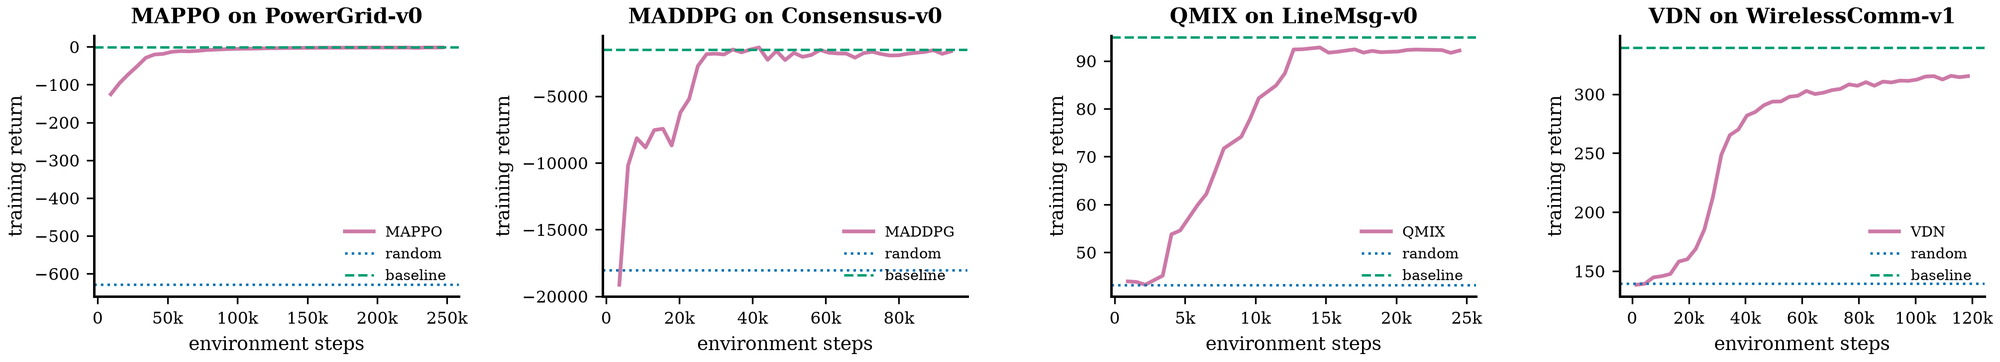
\includegraphics[width=\textwidth]{marl_training.png}
  \caption{Learning curves saved by \code{examples/algorithms/marl\_training\_demo.py}
    (default suite, seed 0): mean return of the exploratory training episodes
    over environment steps, with the evaluation returns of random actions
    (dotted) and of the baseline controller (dashed) for reference. The
    training returns include the random warm-up and the exploration (policy
    noise or $\epsilon$-greedy actions) and are averaged over the few episodes
    that finish in each interval, so they are not directly comparable with
    the evaluation returns of the deterministic policy in
    Table~\ref{tab:marl-demo-results}.}
  \label{fig:marl-training}
\end{figure}

% ---------------------------------------------------------------------------
\section{Adding an algorithm}\label{sec:marl-extending}

A new algorithm reuses the core and implements only what is specific to it.
Inside the package it gets its own module in the folder of its family (or a
new family folder with a \code{common.py} when it shares code with a sibling):

\begin{enumerate}
  \item Define a configuration dataclass that derives from
    \code{OnPolicyConfig} or \code{OffPolicyConfig} (validate new fields in
    \code{\_\_post\_init\_\_}, after calling the parent's).
  \item Subclass \code{OnPolicyAlgorithm} or \code{OffPolicyAlgorithm} and set
    the class attributes \code{name}, \code{action\_kinds} and
    \code{config\_class}.
  \item Implement the hooks: \code{\_build()} (networks and optimisers; it runs
    under the seeded, forked PyTorch generator), \code{act(obs,
    deterministic=False)}, \code{\_modules()} (what \code{save} stores) and,
    for an on-policy method, \code{\_rollout\_step(obs)} and
    \code{\_update(rollout)}, optionally \code{\_rollout\_fields()} and
    \code{\_observe\_transition(transition)}; for an off-policy method,
    \code{\_explore(obs)} and \code{\_update(batch)}. Extra state such as
    normalisers goes into \code{\_extra\_state()} and
    \code{\_load\_extra\_state(state)}. Use \code{self.np\_rng} and
    \code{self.torch\_rng} for all randomness, \code{self.agent\_inputs} for
    per-agent network inputs and \code{PerAgent} for shared or separate
    networks, and batch over copies and agents.
  \item Register it: add an \code{AlgorithmInfo} record (name,
    \code{"module:Class"} entry point, family, action kinds, summary and
    reference) to the tuple in \pkg{marl\_algorithms.registry}, and optionally a
    lazy export in \code{marl\_algorithms/\_\_init\_\_.py}. \code{train},
    \code{make\_algorithm}, \code{Algorithm.load} and \code{marl-train} then
    find it. An unregistered class can still be trained directly
    (\code{MyAlgorithm(envs, seed=0).learn(envs, ...)}) and loaded with
    \code{MyAlgorithm.load(path)}.
  \item Add presets as a table \code{\{name: \{env\_id: preset\}\}} in a
    module of \pkg{marl\_algorithms.presets} and merge it into \code{PRESETS} in
    \code{presets/\_\_init\_\_.py}, where \code{get\_preset}, \code{compare} and
    \code{marl-train presets} look them up.
  \item Add tests in \code{tests/algorithms/}: action shapes on several
    environments, \code{policy()} with \code{env\_lib.evaluate}, the
    \code{TypeError} for an unsupported action kind, a short \code{learn} with
    shared and separate parameters, seed determinism, a \code{save}/\code{load}
    round trip and a loose learning check on a small task.
\end{enumerate}

A minimal skeleton, an independent advantage actor-critic for discrete
actions (one gradient step per rollout on the agents' own rewards):

% norun
\begin{pycode}
from dataclasses import dataclass
from typing import ClassVar

import torch
from torch import nn

from marl_algorithms.core.base import OnPolicyAlgorithm
from marl_algorithms.core.buffers import compute_gae
from marl_algorithms.core.config import OnPolicyConfig
from marl_algorithms.core.networks import CategoricalPolicy, PerAgent, mlp


@dataclass
class A2CConfig(OnPolicyConfig):
    """Options of IA2C (this sketch ignores the normalisation options)."""

    ent_coef: float = 0.01


class IA2C(OnPolicyAlgorithm):
    """Independent advantage actor-critic (discrete actions)."""

    name: ClassVar[str] = "ia2c"
    action_kinds: ClassVar[tuple[str, ...]] = ("discrete",)
    config_class: ClassVar[type[A2CConfig]] = A2CConfig

    def _build(self):
        cfg, spec = self.config, self.spec
        self.actor = PerAgent(
            lambda: CategoricalPolicy(self.agent_input_dim, spec.n_actions,
                                      cfg.hidden_sizes, cfg.activation),
            spec.n_agents, cfg.share_parameters).to(self.device)
        self.critic = PerAgent(
            lambda: mlp(self.agent_input_dim, 1, cfg.hidden_sizes,
                        cfg.activation),
            spec.n_agents, cfg.share_parameters).to(self.device)
        self.params = [*self.actor.parameters(), *self.critic.parameters()]
        self.optimizer = torch.optim.Adam(self.params, lr=cfg.lr)

    def _modules(self):
        return {"actor": self.actor, "critic": self.critic,
                "optimizer": self.optimizer}

    def act(self, obs, deterministic=False):
        inputs = self.agent_inputs(self.tensor(obs))
        with torch.inference_mode():
            if deterministic:
                return self.actor(inputs).argmax(-1).cpu().numpy()
            actions, _ = self.actor.call("sample", inputs, self.torch_rng)
        return actions.cpu().numpy()

    def _rollout_step(self, obs):
        return self.act(obs), {}                 # no extra rollout fields

    def _update(self, rollout):
        cfg = self.config
        inputs = self.agent_inputs(self.tensor(rollout["obs"]))
        values = self.critic(inputs).squeeze(-1)                  # (T, B, n)
        with torch.no_grad():
            next_inputs = self.agent_inputs(self.tensor(rollout["next_obs"]))
            next_values = self.critic(next_inputs).squeeze(-1)
        advantages, returns = compute_gae(
            rollout["agent_rewards"], values.detach().cpu().numpy(),
            next_values.cpu().numpy(), rollout["terminated"],
            rollout["truncated"], cfg.gamma, cfg.gae_lambda)
        actions = self.tensor(rollout["actions"], torch.int64)
        log_prob, entropy = self.actor.call("log_prob", inputs, actions)
        loss = (-(log_prob * self.tensor(advantages)).mean()
                - cfg.ent_coef * entropy.mean()
                + 0.5 * (values - self.tensor(returns)).pow(2).mean())
        self.optimizer.zero_grad(set_to_none=True)
        loss.backward()
        nn.utils.clip_grad_norm_(self.params, cfg.max_grad_norm)
        self.optimizer.step()
        return {"loss": loss.item(), "entropy": entropy.mean().item()}


# Registration (in marl_algorithms/registry.py) and a preset (in a module of
# marl_algorithms/presets/, merged into PRESETS):
# AlgorithmInfo("ia2c", "my_package.ia2c:IA2C", "on-policy", ("discrete",),
#               "independent advantage actor-critic", "<reference>")
PRESETS = {"ia2c": {"LineMsg-v0": {"num_envs": 32, "total_steps": 100_000,
                                   "config": {"lr": 1e-3}, "env_kwargs": {}}}}
\end{pycode}

% ---------------------------------------------------------------------------
\section{References}\label{sec:marl-references}

The source code of \pkg{marl\_algorithms} cites the following publications.

\begin{itemize}[leftmargin=1.5em,itemindent=-1.5em,label={}]
  \item J. Ackermann, V. Gabler, T. Osa and M. Sugiyama (2019).
    \emph{Reducing overestimation bias in multi-agent domains using double
    centralized critics.} NeurIPS Deep RL Workshop, arXiv:1910.01465.
  \item M. Andrychowicz et al.\ (2021). \emph{What matters in on-policy
    reinforcement learning? A large-scale empirical study.} ICLR.
  \item C. S. de Witt, T. Gupta, D. Makoviichuk, V. Makoviychuk,
    P. H. S. Torr, M. Sun and S. Whiteson (2020). \emph{Is independent
    learning all you need in the StarCraft multi-agent challenge?}
    arXiv:2011.09533.
  \item S. Fujimoto, H. van Hoof and D. Meger (2018). \emph{Addressing
    function approximation error in actor-critic methods.} ICML.
  \item T. P. Lillicrap et al.\ (2016). \emph{Continuous control with deep
    reinforcement learning.} ICLR.
  \item R. Lowe, Y. Wu, A. Tamar, J. Harb, P. Abbeel and I. Mordatch (2017).
    \emph{Multi-agent actor-critic for mixed cooperative-competitive
    environments.} NeurIPS.
  \item V. Mnih et al.\ (2015). \emph{Human-level control through deep
    reinforcement learning.} Nature 518, 529--533.
  \item T. Rashid et al.\ (2018). \emph{QMIX: monotonic value function
    factorisation for deep multi-agent reinforcement learning.} ICML.
  \item J. Schulman, P. Moritz, S. Levine, M. Jordan and P. Abbeel (2016).
    \emph{High-dimensional continuous control using generalized advantage
    estimation.} ICLR.
  \item J. Schulman, F. Wolski, P. Dhariwal, A. Radford and O. Klimov (2017).
    \emph{Proximal policy optimization algorithms.} arXiv:1707.06347.
  \item D. Silver et al.\ (2014). \emph{Deterministic policy gradient
    algorithms.} ICML.
  \item P. Sunehag et al.\ (2018). \emph{Value-decomposition networks for
    cooperative multi-agent learning based on team reward.} AAMAS.
  \item M. Tan (1993). \emph{Multi-agent reinforcement learning: independent
    vs.\ cooperative agents.} ICML.
  \item H. van Hasselt, A. Guez and D. Silver (2016). \emph{Deep
    reinforcement learning with double Q-learning.} AAAI.
  \item C. Yu, A. Velu, E. Vinitsky, J. Gao, Y. Wang, A. Bayen and Y. Wu
    (2022). \emph{The surprising effectiveness of PPO in cooperative
    multi-agent games.} NeurIPS Datasets and Benchmarks.
\end{itemize}

\endgroup


\part{Toolkit}
% ---------------------------------------------------------------------------
% Chapter: Toolkit overview and parakit
% ---------------------------------------------------------------------------
\chapter{Toolkit Overview and Parameter Management}\label{chap:toolkit}

The \pkg{toolkit} package collects research utilities that are independent of
the environments. This chapter describes its structure and then documents
\pkg{toolkit.parakit}, the parameter-management module. The plotting and
neural-network subpackages have their own chapters.

\section{Structure of the toolkit}\label{sec:toolkit-structure}

\begin{table}[htbp]
  \centering
  \small
  \caption{Subpackages of \pkg{toolkit}.}
  \label{tab:toolkit-subpackages}
  \begin{tabularx}{\textwidth}{@{}l>{\raggedright\arraybackslash}X>{\raggedright\arraybackslash}p{3.3cm}l@{}}
    \toprule
    Subpackage & Contents & Dependencies & Chapter \\
    \midrule
    \pkg{toolkit.plotkit} & Learning curves, bars, histograms, heatmaps,
      style presets, palettes, figure export, gallery CLI &
      matplotlib (core) & \ref{chap:plotkit} \\
    \pkg{toolkit.neural\_toolkit} & Policy, value and Q-networks, encoders,
      decoders, factories, \code{NetworkUtils}, tabular tools &
      PyTorch (\code{torch} extra) & \ref{chap:neural} \\
    \pkg{toolkit.parakit} & Save, load, validate and apply \pkg{argparse}
      defaults; Tk editor window & standard library; Tk for the window &
      \ref{chap:toolkit} \\
    \bottomrule
  \end{tabularx}
\end{table}

The subpackages are imported lazily: \code{import toolkit} only defines
\code{toolkit.\_\_version\_\_}, and the first access to
\code{toolkit.plotkit}, \code{toolkit.neural\_toolkit} or
\code{toolkit.parakit} imports that subpackage. A script that only plots
therefore never imports PyTorch, and \pkg{parakit}'s headless functions work
on systems without Tk. The usual import style names the subpackage
explicitly:

\begin{pycode}
from toolkit.plotkit import plot_learning_curves, save_figure
from toolkit.parakit import apply_parameters, load_parameters
from toolkit.neural_toolkit import MLPPolicyNetwork, NetworkUtils  # needs torch
\end{pycode}

All three subpackages follow the conventions of the environments: they never
print, never configure logging (diagnostics go to \code{logging} loggers named
after the module), never touch the global random state, and report problems
with exceptions or \code{warnings} whose messages say how to fix them.

\section{parakit: managing argparse parameters}\label{sec:parakit}

Research scripts are usually configured through an
\code{argparse.ArgumentParser}. \pkg{parakit} treats the parser as the single
source of truth for the parameters, their types and their allowed values, and
adds four operations on top of it: reading the current defaults, saving them
to a JSON file, loading a file, and installing validated values as the new
defaults. Because the values become \emph{defaults}, flags given on the
command line still override them. An optional Tk window
(Section~\ref{sec:parakit-gui}) lets users edit the values interactively.

\subsection{Quick start}\label{sec:parakit-quickstart}

The typical workflow saves the configuration of a run next to its results and
later restores it:

\begin{pycode}
import argparse
from toolkit.parakit import (
    apply_parameters, get_parameters, load_parameters, save_parameters,
)

parser = argparse.ArgumentParser()
parser.add_argument("--lr", type=float, default=3e-4, help="learning rate")
parser.add_argument("--batch_size", type=int, default=64)
parser.add_argument("--optimizer", choices=["adam", "sgd"], default="adam")
parser.add_argument("--hidden", type=int, nargs="+", default=[256, 256])
parser.add_argument("--layer_norm", action="store_true")
parser.add_argument("--checkpoint", default=None)

# Save the current defaults into a directory (timestamped file name).
path = save_parameters(get_parameters(parser), "runs/params")

# Later: load the newest file of the directory and install it as defaults.
apply_parameters(parser, load_parameters("runs/params"))

# Values given as text are converted according to the parser.
apply_parameters(parser, {"lr": "1e-3", "hidden": "64 64", "layer_norm": "yes"})
args = parser.parse_args([])            # lr=0.001, hidden=[64, 64], layer_norm=True
args = parser.parse_args(["--lr", "0.01"])  # command-line flags still win
\end{pycode}

\subsection{Headless API}\label{sec:parakit-api}

Table~\ref{tab:parakit-api} lists the functions; none of them needs Tk.

\begin{table}[htbp]
  \centering
  \small
  \caption{Headless functions of \pkg{toolkit.parakit}.}
  \label{tab:parakit-api}
  \begin{tabularx}{\textwidth}{@{}>{\raggedright\arraybackslash}p{5.6cm}>{\raggedright\arraybackslash}X@{}}
    \toprule
    Function & Description \\
    \midrule
    \code{get\_parameters(parser)} &
      Dictionary \code{\{dest: default\}} of all tunable options (lists are
      copied). \\
    \code{save\_parameters(values, path\_or\_dir)} &
      Write \code{values} as JSON and return the \code{Path} of the file.
      A path with a suffix is used as the file name; a directory (existing, or
      a path without suffix) receives a new timestamped file. Parent
      directories are created and the write is atomic. \\
    \code{load\_parameters(path)} &
      Read a JSON object from a file, or from the newest
      \code{parameters\_*.json} file of a directory. Raises
      \code{FileNotFoundError} or \code{ValueError}. \\
    \code{apply\_parameters(parser, values, strict=True, validation\_callbacks=None)} &
      Convert and validate every value with \code{parse\_value}, then call
      \code{parser.set\_defaults}. Returns the parser. \\
    \code{parse\_value(action, text, validator=None)} &
      Convert one value (text or an already typed JSON value) for an
      \pkg{argparse} action; see Section~\ref{sec:parakit-parsing}. \\
    \code{parse\_bool(value)} &
      Convert \code{true/false}, \code{yes/no}, \code{on/off}, \code{1/0}
      (any case) or a boolean to \code{bool}. \\
    \code{format\_value(action, value)} &
      Text that \code{parse\_value} converts back (lists as JSON, \code{None}
      as \code{"None"}). \\
    \code{describe\_type(action)} &
      Short type description such as \code{"float"}, \code{"list[int]"} or
      \code{"str or None"}. \\
    \code{tunable\_actions(parser)} &
      Dictionary \code{\{dest: action\}} of the options \pkg{parakit}
      manages. \\
    \bottomrule
  \end{tabularx}
\end{table}

\paragraph{Tunable options.}
\code{tunable\_actions} skips help, version and sub-parser actions and options
whose destination or default is \code{argparse.SUPPRESS}. When several options
share a destination, such as a \code{--flag}/\code{--no-flag} pair, the first
one is used. Positional arguments are included and keyed by their name.

\paragraph{Errors.}
\code{apply\_parameters} either applies all values or none. With
\code{strict=True} (the default) a key that is not a parser destination raises
a \code{ValueError} that lists the unknown keys and the valid names; with
\code{strict=False} unknown keys are ignored. Otherwise every value is
converted, and all conversion and validation failures are reported together
in one \code{ValueError}, one line per parameter. The parser is left unchanged
whenever an exception is raised.

\subsection{File format}\label{sec:parakit-format}

A parameter file is a flat JSON object that maps each destination name
(\code{action.dest}) to its value, written in UTF-8 with an indentation of four
spaces:

\begin{textcode}
{
    "lr": 0.001,
    "batch_size": 64,
    "optimizer": "adam",
    "hidden": [
        64,
        64
    ],
    "layer_norm": true,
    "checkpoint": null
}
\end{textcode}

\begin{itemize}
  \item \emph{File names.} Saving into a directory creates
    \code{parameters\_YYYYmmdd\_HHMMSS.json}; if that name exists (two saves in
    the same second), \code{\_1}, \code{\_2}, \ldots\ is appended. Loading from
    a directory reads the file whose name sorts last, which is the most recent
    one.
  \item \emph{Values.} JSON numbers, strings, booleans, \code{null} and lists
    are stored as such. NumPy arrays and scalars are converted with
    \code{tolist()}, sets are stored as sorted lists and any other object as its
    \code{str()}.
  \item \emph{Loading.} Values read from a file pass through the same
    conversion as text, so a file may contain \code{"64"} or \code{64} for an
    integer option, and \code{"yes"} or \code{true} for a flag. A file may
    contain a subset of the parameters; the other defaults are kept.
  \item \emph{Atomic writes.} Files are written to a temporary file in the
    target directory and renamed, so an interrupted save never leaves a
    truncated file behind.
\end{itemize}

\subsection{Parsing rules}\label{sec:parakit-parsing}

\code{parse\_value(action, text)} derives the conversion from the parser's
own declarations, so the same rules apply to values typed in the editor
window, loaded from JSON or passed to \code{apply\_parameters}.
Table~\ref{tab:parakit-rules} summarises them.

\begin{table}[htbp]
  \centering
  \small
  \caption{Conversion rules of \code{parse\_value}.}
  \label{tab:parakit-rules}
  \begin{tabularx}{\textwidth}{@{}>{\raggedright\arraybackslash}p{4.4cm}>{\raggedright\arraybackslash}X@{}}
    \toprule
    Declaration & Accepted input and result \\
    \midrule
    \code{type=callable} &
      The callable is applied to text (surrounding blanks are removed for
      \code{int} and \code{float}). Already typed values from JSON are checked:
      an \code{int} option accepts \code{3} and \code{3.0} but not \code{3.5};
      a \code{float} option accepts integers. \\
    No \code{type} &
      The type is inferred from the default (\code{bool}, \code{int},
      \code{float}, otherwise \code{str}), or from the \code{choices} when all
      have the same type. \\
    Booleans: \code{store\_true}, \code{store\_false},
      \code{BooleanOptionalAction}, \code{type=bool} or a boolean default &
      \code{true/false}, \code{yes/no}, \code{on/off}, \code{1/0} in any case,
      or a JSON boolean. The string \code{"False"} gives \code{False}. \\
    Lists: \code{nargs="+"}, \code{"*"}, an integer, \code{append} and
      \code{extend} actions &
      A JSON list (\code{[1.0, 2.0]}), a Python literal list or tuple, or
      tokens separated by commas (if the text contains a comma) or by
      whitespace. Each element is converted; \code{"+"} requires at least one
      element and an integer \code{nargs} exactly that many. \\
    Default \code{None} or \code{nargs="?"} &
      \code{None}, \code{null} (any case) and the empty string give
      \code{None}. For other options \code{None} is rejected, except that a
      string option accepts the text \code{"None"} literally. \\
    \code{choices} &
      Enforced on the converted value (on every element of a list). \\
    \code{count} action & Converted as an integer. \\
    \bottomrule
  \end{tabularx}
\end{table}

\paragraph{Declare types explicitly.}
Type inference from the default is a convenience of \pkg{parakit}, not of
\pkg{argparse}. An option declared as \code{add\_argument("--gamma",
default=0.99)} is converted to \code{float} by \pkg{parakit}, but
\code{parser.parse\_args(["--gamma", "0.9"])} returns the \emph{string}
\code{"0.9"}. Give every option a \code{type=} so that both paths agree.

\paragraph{Validation callbacks.}
A validator receives the \emph{converted} value and signals the result in one
of the following ways: return \code{True}/\code{False}; return a tuple
\code{(is\_valid, message)} or the legacy form \code{(is\_valid,
converted\_value, message)}; return \code{None} (valid); or raise
\code{ValueError} or \code{TypeError}, whose text becomes the error message.
Validators are not called when the converted value is \code{None}, and a value
returned by a validator is ignored: the result always follows the parser
declaration.

\begin{pycode}
def positive_even(value):
    return value > 0 and value % 2 == 0, "batch size must be a positive even number"

validators = {"batch_size": positive_even,
              "lr": lambda v: (0 < v <= 1, "lr must lie in (0, 1]")}
apply_parameters(parser, {"batch_size": "128", "lr": 0.01},
                 validation_callbacks=validators)

try:
    apply_parameters(parser, {"batch_size": 7, "optimizer": "rmsprop"},
                     validation_callbacks=validators)
except ValueError as exc:
    print(exc)
# Invalid parameter values:
# batch_size: batch size must be a positive even number
# optimizer: 'rmsprop' is not a valid choice; value must be one of: 'adam', 'sgd'
\end{pycode}

\subsection{Recommended workflow in training scripts}\label{sec:parakit-workflow}

The following pattern gives a script three configuration layers with a clear
precedence: parser defaults, then an optional parameter file, then explicit
command-line flags.

\begin{pycode}
import argparse
import sys
from toolkit.parakit import apply_parameters, get_parameters, load_parameters, save_parameters

def build_parser():
    parser = argparse.ArgumentParser()
    parser.add_argument("--config", default=None, help="JSON file or directory")
    parser.add_argument("--lr", type=float, default=3e-4)
    parser.add_argument("--seed", type=int, default=0)
    return parser

def main(argv=None):
    parser = build_parser()
    pre, _ = parser.parse_known_args(argv)          # read --config first
    if pre.config is not None:
        apply_parameters(parser, load_parameters(pre.config), strict=False)
    args = parser.parse_args(argv)                  # flags override the file
    run_dir = f"runs/seed{args.seed}"
    save_parameters(vars(args), f"{run_dir}/config.json")
    return args

main(["--lr", "0.001"])
\end{pycode}

\code{AJLATTConfig.add\_arguments(parser)} registers every AJLATT option on a
parser (Chapter~\ref{chap:ajlatt}), so environment parameters can be managed
in the same way.

\subsection{The ParameterTuner window}\label{sec:parakit-gui}

\code{ParameterTuner} opens a Tk window with one input field per tunable
option: a check box for booleans, a drop-down list for options with
\code{choices}, and a text field otherwise. Each field shows the option's help
text and its type as reported by \code{describe\_type}. Values are validated
with \code{parse\_value} (and the optional validation callbacks), written to
timestamped JSON files, and installed as the parser's defaults when the window
closes.

\begin{table}[htbp]
  \centering
  \small
  \caption{Constructor arguments of \code{ParameterTuner}.}
  \label{tab:parakit-tuner}
  \begin{tabularx}{\textwidth}{@{}>{\raggedright\arraybackslash}p{3.8cm}>{\raggedright\arraybackslash}p{2.1cm}>{\raggedright\arraybackslash}X@{}}
    \toprule
    Argument & Default & Meaning \\
    \midrule
    \code{parser} & required & The \code{argparse.ArgumentParser} to tune. \\
    \code{save\_delay} & \code{30000} & Auto-save interval in milliseconds. \\
    \code{save\_path} & \code{None} & Output directory for the JSON files; \code{None}
      uses the current working directory. Created on the first save. \\
    \code{auto\_save\_enabled} & \code{True} & Start with auto-save switched on. \\
    \code{validation\_callbacks} & \code{None} & Per-destination validators
      (Section~\ref{sec:parakit-parsing}); callbacks for unknown names are
      ignored with a warning. \\
    \code{inactivity\_timeout} & \code{10} & Seconds without keyboard or mouse
      activity after which the values are saved and the window closes;
      \code{None} disables the automatic close. \\
    \bottomrule
  \end{tabularx}
\end{table}

\paragraph{Window behaviour.}
\begin{itemize}
  \item \emph{Save Parameters} validates all fields and writes a new file.
    Invalid values are listed in an error dialog and nothing is saved.
  \item \emph{OK} saves and closes the window; if the values are invalid the
    window stays open.
  \item \emph{Auto-save} (check box) saves every \code{save\_delay}
    milliseconds while enabled; problems are shown in the status line instead
    of dialogs.
  \item After \code{inactivity\_timeout} seconds without activity the window
    saves (if the values are valid) and closes. The default of ten seconds
    suits scripts that open the window at start-up and should continue
    unattended; pass a larger value or \code{None} for interactive editing.
  \item \emph{Browse} selects another output directory and \emph{Reset to
    Default} returns to the initial one. Closing the window with the window
    manager does not save.
\end{itemize}

\code{tune()} blocks until the window closes and returns the parser. The
values of the last \emph{successful} save (manual, OK, auto-save or
inactivity save) become the parser's defaults; if nothing was saved, the
parser is unchanged. The path of the last file is available as
\code{tuner.last\_saved\_path}. The class method
\code{ParameterTuner.tune\_parameters(parser, ...)} creates a tuner, calls
\code{tune()} and returns the parser; \code{ParameterAdjuster} is a
backward-compatible alias of the class. The font of the window is the class
attribute \code{font\_family} (default \code{"Times New Roman"}).

% norun
\begin{pycode}
from toolkit.parakit import ParameterTuner

tuner = ParameterTuner(parser, save_path="runs/params", inactivity_timeout=None,
                       validation_callbacks=validators)
parser = tuner.tune()                  # blocks until the window is closed
args = parser.parse_args()
print("saved to", tuner.last_saved_path)
\end{pycode}

\paragraph{Systems without Tk or without a display.}
\code{tune()} raises \code{ImportError} with installation instructions when
Tk is missing (the message is available as
\code{toolkit.parakit.TK\_MISSING\_MESSAGE}) and \code{RuntimeError} when no
display is available, for example on a cluster node or over SSH without X
forwarding. Scripts that should run everywhere catch both exceptions and fall
back to the headless API:

% norun
\begin{pycode}
try:
    ParameterTuner(parser, save_path="runs/params").tune()
except (ImportError, RuntimeError) as exc:
    print(f"Editor not available ({exc}); using the current defaults.")
\end{pycode}

The script \code{examples/parakit\_demo.py} demonstrates the complete
workflow, including the window (\code{--gui}), loading a file or directory
(\code{--load}) and command-line overrides (\code{--set KEY=VALUE}).

% ---------------------------------------------------------------------------
% Chapter: plotkit
% ---------------------------------------------------------------------------
\chapter{plotkit: Publication-Quality Plots}\label{chap:plotkit}
% Long monospaced identifiers leave little room for line breaking; allow some
% extra inter-word stretch in this chapter (the group keeps it local).
\begingroup\setlength{\emergencystretch}{3em}% chapter-local

\pkg{toolkit.plotkit} produces the figures that research papers on
reinforcement learning need most often: learning curves aggregated over seeds
with uncertainty bands, grouped bar charts with error bars, histograms and
annotated heatmaps. It depends only on matplotlib, accepts data from NumPy,
pandas, PyTorch, TensorFlow and JAX, and never changes the global matplotlib
configuration unless explicitly asked to.

\begin{figure}[htbp]
  \centering
  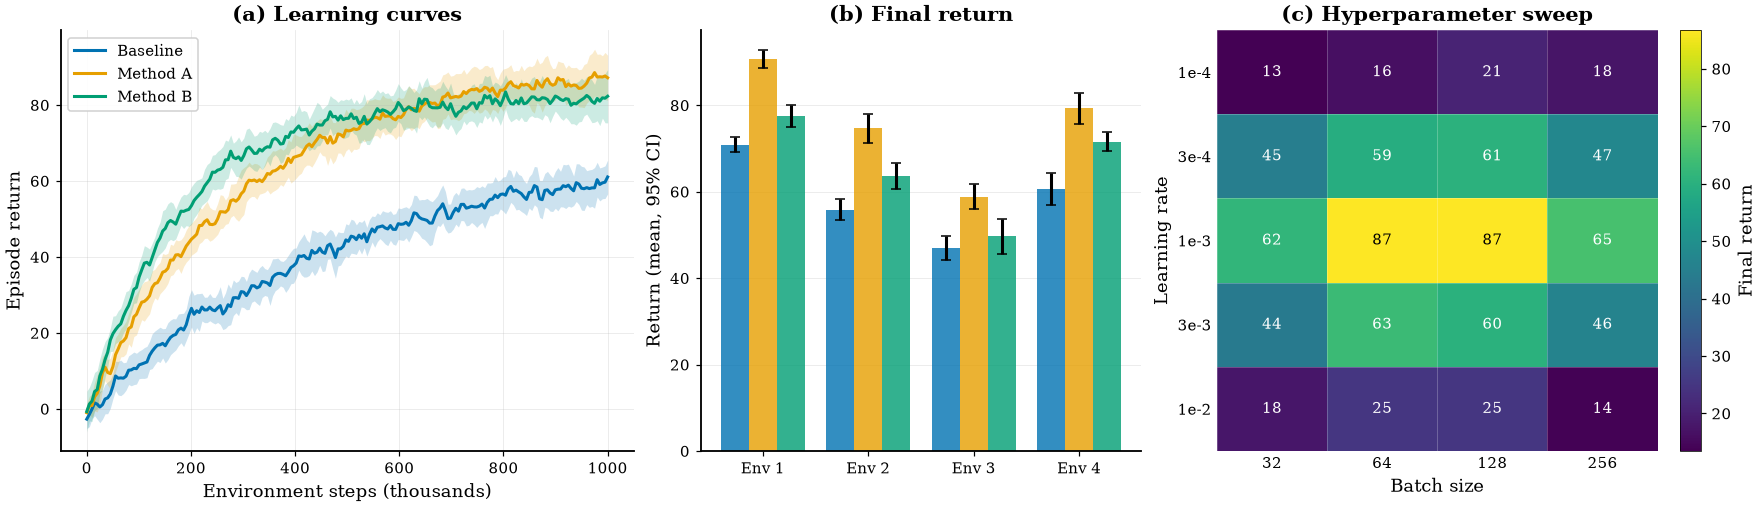
\includegraphics[width=\textwidth]{plotkit_gallery.png}
  \caption{A three-panel summary figure made with \pkg{plotkit}
    (\code{examples/plotkit\_gallery.py}, synthetic data): (a) learning curves
    of three methods over eight seeds with 95\,\% confidence bands and EMA
    smoothing, (b) grouped bars with 95\,\% confidence intervals, (c) an
    annotated heatmap of a hyperparameter sweep. Each method keeps its
    Okabe-Ito colour in every panel.}
  \label{fig:plotkit-gallery}
\end{figure}

\section{Overview}\label{sec:plotkit-overview}

\begin{table}[htbp]
  \centering
  \small
  \caption{Public API of \pkg{toolkit.plotkit}.}
  \label{tab:plotkit-api}
  \begin{tabularx}{\textwidth}{@{}>{\raggedright\arraybackslash}p{4.4cm}>{\raggedright\arraybackslash}X@{}}
    \toprule
    Name & Purpose \\
    \midrule
    \code{plot\_shadow\_curve} & Mean curves with a shaded band (std, SEM, 95\,\% CI, min-max or explicit) and optional smoothing. \\
    \code{plot\_learning\_curves} & \code{\{method: runs\}} learning curves aggregated over seeds; runs may have different lengths. \\
    \code{plot\_line}, \code{plot\_scatter} & Line and scatter plots of one or several series. \\
    \code{plot\_bar} & Bar charts; several series are grouped side by side, with error bars and value labels. \\
    \code{plot\_histogram} & Overlaid histograms on common bins. \\
    \code{plot\_heatmap}, \code{plot\_gray\_scale} & Annotated heatmaps with colorbar (seaborn-compatible arguments, matplotlib only). \\
    \code{save\_figure} & Save a figure to several formats at once. \\
    \code{style\_context}, \code{set\_research\_style}, \code{reset\_style}, \code{STYLE\_PRESETS} & Style presets applied locally or globally. \\
    \code{get\_palette}, \code{RESEARCH\_COLORS}, \code{OKABE\_ITO\_COLORS} (and the \code{*\_COLOR\_LIST} variants) & Colour palettes, including a colour-blind-safe one. \\
    \bottomrule
  \end{tabularx}
\end{table}

All plot functions share the same behaviour:
\begin{itemize}
  \item they draw into the \code{ax} argument when it is given and otherwise
    create a new figure of size \code{figsize};
  \item they apply the \code{style} preset \emph{locally}, inside a
    \code{matplotlib.rc\_context}, so the caller's \code{rcParams} are
    unchanged afterwards;
  \item they return the \code{matplotlib.axes.Axes} they drew on, which can be
    customised further with ordinary matplotlib calls.
\end{itemize}

A non-default style also restyles the axes it draws on (spines, tick labels,
axis-label fonts), so that axes created outside the style context match the
preset. Pass \code{style="default"} to leave an existing axes exactly as it
is.

\begin{pycode}
import numpy as np
from toolkit.plotkit import plot_shadow_curve, save_figure

rng = np.random.default_rng(0)
returns = rng.normal(size=(5, 100)).cumsum(axis=1)     # 5 seeds x 100 steps
ax = plot_shadow_curve(returns, band="ci95", smoothing=10, labels="Agent",
                       xlabel="Episode", ylabel="Return")
save_figure(ax, "renders/first_curve", formats=("pdf", "png"))
\end{pycode}

\section{Input rules}\label{sec:plotkit-inputs}

Every function converts its data inputs with the same rules:

\begin{itemize}
  \item A 1-D array-like of numbers, including a flat Python list of scalars,
    is \emph{one} series.
  \item A list or tuple of array-likes is \emph{several} series, one per
    element; the elements may have different lengths.
  \item A 2-D array is read by the function: \code{plot\_shadow\_curve} reads
    it as \emph{samples of one curve} along \code{axis} (default: rows are
    samples such as seeds, columns are steps); \code{plot\_line},
    \code{plot\_scatter}, \code{plot\_bar} and \code{plot\_histogram} read it
    as \code{(n\_series, n\_points)}.
  \item A pandas \code{DataFrame} contributes one series per column.
  \item pandas \code{Series}, PyTorch tensors (on any device, with or without
    \code{requires\_grad}), TensorFlow eager tensors and JAX arrays are
    converted to NumPy automatically. Masked arrays become NaN.
  \item A single \code{x} is shared by all series; a list of arrays (or a 2-D
    array) gives one \code{x} per series. When \code{x} is omitted, each series
    is plotted against \code{0, \ldots, n - 1}.
\end{itemize}

Length mismatches raise a \code{ValueError} that states both shapes and, when
a 2-D input looks transposed, suggests transposing it. To pass a nested list
as a single 2-D sample matrix to \code{plot\_shadow\_curve}, convert it with
\code{np.asarray} first; otherwise it is read as several curves.

\section{Common parameters}\label{sec:plotkit-common}

The parameters in Table~\ref{tab:plotkit-common} have the same meaning in all
plot functions (the heatmap functions have no \code{labels}, \code{colors},
\code{legend} or \code{grid}).

\begin{table}[htbp]
  \centering
  \small
  \caption{Parameters shared by the plot functions.}
  \label{tab:plotkit-common}
  \begin{tabularx}{\textwidth}{@{}>{\raggedright\arraybackslash}p{2.6cm}>{\raggedright\arraybackslash}p{2.5cm}>{\raggedright\arraybackslash}X@{}}
    \toprule
    Parameter & Default & Meaning \\
    \midrule
    \code{labels} & \code{None} & Legend labels, one per series; default \code{"Curve 1"}, \code{"Series 1"}, \ldots. A wrong count gives a warning. \\
    \code{colors} & \code{None} & \code{None} (the style's colour cycle), one colour, a list of colours (cycled), a palette name (\code{"okabe\_ito"}, \code{"research"}, \ldots) or a matplotlib colormap name. \\
    \code{ax} & \code{None} & Axes to draw on; a new figure is created when \code{None}. \\
    \code{figsize} & \code{(10, 6)} & Size in inches of a new figure (\code{(8, 6)} for heatmaps). \\
    \code{title}, \code{xlabel}, \code{ylabel} & \code{None} & Axes title and axis labels. \\
    \code{legend} & \code{True} & Show a legend when there are several series or labels were given; a string sets the location, e.g. \code{"lower right"}. \\
    \code{grid} & \code{True} & Draw a major grid (only along the value axis for bars and histograms). \\
    \code{style} & \code{"research"} & Style preset applied locally (Section~\ref{sec:plotkit-styles}), a matplotlib style name, a dict of \code{rcParams}, or \code{None}. \\
    \code{**kwargs} & & Passed to the underlying matplotlib call (\code{plot}, \code{scatter}, \code{bar}, \code{hist}, \code{imshow}); \code{color} and \code{label} are accepted as aliases of \code{colors} and \code{labels}. \\
    \bottomrule
  \end{tabularx}
\end{table}

\section{Curves with uncertainty bands}\label{sec:plotkit-curves}

\subsection{plot\_shadow\_curve}

% norun
\begin{pycode}
plot_shadow_curve(y, x=None, y_std=None, labels=None, colors=None, alpha=0.2,
                  ax=None, axis=0, figsize=(10, 6), title=None, xlabel=None,
                  ylabel=None, legend=True, grid=True, style="research",
                  legend_labels=None, x_tick_labels=None, y_tick_labels=None,
                  *, band="std", smoothing=None, **kwargs) -> Axes
\end{pycode}

Each element of \code{y} gives one curve. A 2-D element holds samples of the
curve (for example one row per seed) and is drawn as its mean with a band; a
1-D element is drawn as it is, with a band only when \code{y\_std} is given.

\begin{table}[htbp]
  \centering
  \small
  \caption{Parameters specific to \code{plot\_shadow\_curve}.}
  \label{tab:plotkit-shadow}
  \begin{tabularx}{\textwidth}{@{}>{\raggedright\arraybackslash}p{2.8cm}>{\raggedright\arraybackslash}p{1.6cm}>{\raggedright\arraybackslash}X@{}}
    \toprule
    Parameter & Default & Meaning \\
    \midrule
    \code{y} & required & One or several curves (see the input rules). \\
    \code{x} & \code{None} & Shared x values or one array per curve. \\
    \code{y\_std} & \code{None} & Explicit half-width of the band: a scalar, one array for all curves, or one entry per curve (entries may be \code{None}). Overrides \code{band}. \\
    \code{alpha} & \code{0.2} & Band opacity; \code{0} hides the band. \\
    \code{axis} & \code{0} & Sample axis of 2-D inputs: \code{0} means rows are samples and columns are steps; use \code{1} for the transposed layout. \\
    \code{band} & \code{"std"} & \code{"std"}, \code{"sem"}, \code{"ci95"}, \code{"minmax"} or \code{None} (see below). Keyword only. \\
    \code{smoothing} & \code{None} & \code{int}: trailing moving-average window; \code{float} in $(0,1)$: EMA weight. Keyword only. \\
    \code{legend\_labels} & \code{None} & Alias of \code{labels} (takes precedence). \\
    \code{x\_tick\_labels}, \code{y\_tick\_labels} & \code{None} & Custom tick labels: a mapping \code{\{position: label\}}, or a sequence (one label per x value of the first curve, otherwise spread evenly over the data range). \\
    \bottomrule
  \end{tabularx}
\end{table}

\paragraph{Bands.}
Let $y_{i,t}$ be sample $i$ (for example seed $i$) at step $t$, and let
$\mathcal{I}_t$ be the set of samples that are not NaN at step $t$, with
$n_t = |\mathcal{I}_t|$. The drawn curve is the mean
\begin{equation}
  \bar{y}_t = \frac{1}{n_t} \sum_{i \in \mathcal{I}_t} y_{i,t},
\end{equation}
and the band is $[\bar{y}_t - h_t,\, \bar{y}_t + h_t]$ with
\begin{align}
  \texttt{"std"}:\quad  h_t &= \sigma_t = \sqrt{\frac{1}{n_t}\sum_{i \in \mathcal{I}_t} (y_{i,t} - \bar{y}_t)^2}, \\
  \texttt{"sem"}:\quad  h_t &= \frac{s_t}{\sqrt{n_t}}, \qquad
     s_t = \sqrt{\frac{1}{n_t - 1}\sum_{i \in \mathcal{I}_t} (y_{i,t} - \bar{y}_t)^2}, \\
  \texttt{"ci95"}:\quad h_t &= z_{0.975}\,\frac{s_t}{\sqrt{n_t}}, \qquad z_{0.975} \approx 1.96,
\end{align}
while \code{"minmax"} draws $[\min_{i} y_{i,t},\, \max_{i} y_{i,t}]$ over
$\mathcal{I}_t$. The \code{"std"} band uses the population standard deviation;
the SEM-based bands use the sample standard deviation and are undefined (not
drawn) where fewer than two samples exist. The \code{"ci95"} band is the
normal approximation of a 95\,\% confidence interval of the mean; with few
seeds (fewer than about ten) it is narrower than the exact Student-$t$
interval, a fact worth stating in a figure caption. Because the statistics
ignore NaN, runs of different length can be padded with NaN.

\paragraph{Smoothing.}
Smoothing is applied along the step axis \emph{after} the statistics, with the
same filter for the mean and both band edges. An integer $w \geq 1$ selects a
trailing moving average with the same output length; the window shrinks at
the start of the series:
\begin{equation}
  \tilde{y}_t = \frac{1}{|W_t|} \sum_{s \in W_t} y_s, \qquad
  W_t = \{\, s : \max(0, t - w + 1) \le s \le t,\ y_s \text{ finite} \,\}.
\end{equation}
A float $\beta \in (0, 1)$ selects a debiased exponential moving average with
smoothing weight $\beta$, the convention of TensorBoard's smoothing slider
(larger values are smoother):
\begin{equation}
  \tilde{y}_t = \frac{\sum_{s \le t,\ y_s \text{ finite}} \beta^{\,t-s}\, y_s}
                     {\sum_{s \le t,\ y_s \text{ finite}} \beta^{\,t-s}} .
\end{equation}
The normalisation removes the bias towards zero of the plain recursion
$m_t = \beta m_{t-1} + (1-\beta) y_t$, $m_{-1} = 0$; for finite data the
result equals \code{pandas.Series(y).ewm(alpha=1 - beta).mean()}. Non-finite
values are skipped. Note that smoothing the band edges does not turn them into a
confidence band of the smoothed curve; it is a visual aid.

\subsection{plot\_learning\_curves}

% norun
\begin{pycode}
plot_learning_curves(runs, x=None, *, band="ci95", smoothing=None, colors=None,
                     alpha=0.2, ax=None, figsize=(10, 6), title=None,
                     xlabel="Step", ylabel="Return", legend=True, grid=True,
                     style="research", **kwargs) -> Axes
\end{pycode}

\code{runs} maps a method name to its results: a 2-D array
\code{(n\_seeds, n\_steps)}, a 1-D array (a single seed), or a list of 1-D
arrays of possibly different lengths, which are padded with NaN. \code{x} is
either shared or a mapping \code{\{method: x\}}. The function is a thin layer
over \code{plot\_shadow\_curve} with a 95\,\% confidence band by default, and
always shows the legend when \code{legend} is true.

\section{Lines, scatter plots, bars and histograms}\label{sec:plotkit-basic}

\code{plot\_line(x, y, ...)} and \code{plot\_scatter(x, y, ...)} draw one or
several series with the input rules of Section~\ref{sec:plotkit-inputs}.
\code{plot\_scatter} uses \code{s=50} and \code{alpha=0.7} unless they are
given; passing per-point values \code{c=...} (for a colormap)
disables the series colour.

\subsection{plot\_bar}

% norun
\begin{pycode}
plot_bar(x, height, labels=None, colors=None, ax=None, figsize=(10, 6),
         title=None, xlabel=None, ylabel=None, legend=True, grid=True,
         style="research", *, width=0.8, yerr=None, value_labels=False,
         horizontal=False, capsize=3.0, **kwargs) -> Axes
\end{pycode}

\begin{table}[htbp]
  \centering
  \small
  \caption{Parameters specific to \code{plot\_bar}.}
  \label{tab:plotkit-bar}
  \begin{tabularx}{\textwidth}{@{}>{\raggedright\arraybackslash}p{2.6cm}>{\raggedright\arraybackslash}p{1.6cm}>{\raggedright\arraybackslash}X@{}}
    \toprule
    Parameter & Default & Meaning \\
    \midrule
    \code{x} & required & Category labels (strings or numbers), or \code{None} for the indices. Bars are placed at \code{0, \ldots, n\_categories - 1}. \\
    \code{height} & required & One series (1-D), a list of series, or a 2-D array \code{(n\_series, n\_categories)}. Several series are grouped side by side. \\
    \code{width} & \code{0.8} & Total width of a group in category units; each bar is \code{width / n\_series} wide. \\
    \code{yerr} & \code{None} & Error bars: a scalar, one array per series (or one shared array), or a \code{(2, n\_categories)} array of lower and upper errors for a single series. \\
    \code{value\_labels} & \code{False} & Annotate the bars: \code{True} (format \code{".3g"}), a format string such as \code{".1f"}, \code{"\{:.1\%\}"} or \code{"\%.2f"}, or a callable. \\
    \code{horizontal} & \code{False} & Horizontal bars, first category at the top. \\
    \code{capsize} & \code{3.0} & Error-bar cap size in points. \\
    \code{colors} & \code{None} & As usual; for a single series a list with one colour per category colours each bar. \\
    \bottomrule
  \end{tabularx}
\end{table}

\subsection{plot\_histogram}

\code{plot\_histogram(data, bins="auto", ...)} overlays one histogram per
series; its keyword-only arguments are \code{density=False},
\code{alpha=0.45} and \code{histtype="stepfilled"}. The bin
edges are computed once from the pooled data (\code{numpy.histogram\_bin\_edges})
so that all series share the same bins; NaN and infinite values are dropped.
\code{density=True} normalises each histogram to unit area, and the default
y-label is \code{"Density"} or \code{"Count"} accordingly. For the filled
types the fill uses \code{alpha} while the outline stays opaque.

\section{Heatmaps}\label{sec:plotkit-heatmaps}

% norun
\begin{pycode}
plot_heatmap(data, xlabels=None, ylabels=None, cmap="viridis", annot=False,
             ax=None, figsize=(8, 6), title=None, xlabel=None, ylabel=None,
             cbar=True, cbar_label=None, style="research", *, fmt=None,
             vmin=None, vmax=None, center=None, robust=False, mask=None,
             nan_color=None, aspect="auto", square=False, linewidths=None,
             linecolor="white", annot_kws=None, cbar_kws=None, **kwargs) -> Axes
\end{pycode}

\code{plot\_heatmap} draws a 2-D array with row 0 at the top (a 1-D array is
drawn as one row). It is implemented with matplotlib's \code{imshow} and
accepts the most common seaborn arguments, so existing seaborn calls usually
work unchanged.

\begin{table}[htbp]
  \centering
  \small
  \caption{Parameters specific to \code{plot\_heatmap}.}
  \label{tab:plotkit-heatmap}
  \begin{tabularx}{\textwidth}{@{}>{\raggedright\arraybackslash}p{2.8cm}>{\raggedright\arraybackslash}p{1.9cm}>{\raggedright\arraybackslash}X@{}}
    \toprule
    Parameter & Default & Meaning \\
    \midrule
    \code{xlabels}, \code{ylabels} & \code{None} & One tick label per column / row. \code{None} labels cells with their index (up to 30 cells, otherwise automatic integer ticks); \code{False} hides the ticks. Long x labels are rotated. seaborn's \code{xticklabels} / \code{yticklabels} are aliases. \\
    \code{cmap} & \code{"viridis"} & Colormap name or object; use a diverging map (\code{"RdBu\_r"}) with \code{center}. \\
    \code{annot} & \code{False} & \code{True} writes each value into its cell; an array of the same shape writes its entries instead. Text is black or white, whichever contrasts better with the cell colour. \\
    \code{fmt} & \code{None} & Annotation format (\code{".2g"}, \code{"\{:.1\%\}"}, \code{"\%.2f"} or a callable). Default \code{".0f"} for integer-valued data, else \code{".2g"}. \\
    \code{cbar}, \code{cbar\_label} & \code{True}, \code{None} & Colorbar and its label (also \code{cbar\_kws=\{"label": ...\}}). The colorbar is available as \code{ax.images[-1].colorbar}. \\
    \code{vmin}, \code{vmax} & \code{None} & Colour limits (default: data range). \\
    \code{center} & \code{None} & Value mapped to the middle of the colormap; missing limits are chosen symmetrically around it. \\
    \code{robust} & \code{False} & Use the 2nd and 98th percentiles for missing limits. \\
    \code{mask} & \code{None} & Boolean array; cells where it is \code{True} are hidden. \\
    \code{nan\_color} & \code{None} & Colour of NaN and masked cells (default transparent). \\
    \code{aspect}, \code{square} & \code{"auto"}, \code{False} & Cell aspect ratio; \code{square=True} equals \code{aspect="equal"}. \\
    \code{linewidths}, \code{linecolor} & \code{None}, \code{"white"} & Lines between cells; by default 0.5 for matrices of up to 50 cells per side and none for larger ones. \\
    \code{annot\_kws}, \code{cbar\_kws} & \code{None} & Text properties of the annotations (a \code{color} entry disables the automatic contrast colour) and arguments of \code{Figure.colorbar}. \\
    \bottomrule
  \end{tabularx}
\end{table}

\code{plot\_gray\_scale(data, ...)} is \code{plot\_heatmap} with
\code{cmap="gray"} (black is low, white is high), convenient for images,
occupancy grids and attention maps; it accepts all keyword arguments of
\code{plot\_heatmap}.

\section{Styles}\label{sec:plotkit-styles}

A style preset is a set of \code{rcParams} overrides applied on top of the
active configuration. Table~\ref{tab:plotkit-styles} summarises the presets;
\code{STYLE\_PRESETS[name]} is a read-only view of the exact values.

\begin{table}[htbp]
  \centering
  \small
  \caption{Style presets. Font sizes are in points.}
  \label{tab:plotkit-styles}
  \begin{tabular}{@{}lllll@{}}
    \toprule
     & \code{"research"} & \code{"presentation"} & \code{"minimal"} & \code{"default"} \\
    \midrule
    Font family          & serif & sans-serif & sans-serif & unchanged \\
    Base / label size    & 12 / 12 & 16 / 18 & 10 / 10 & unchanged \\
    Title size, weight   & 14, bold & 20, bold & 11, normal & unchanged \\
    Tick / legend size   & 10 / 10 & 14 / 14 & 9 / 9 & unchanged \\
    Line width           & 2.0 & 3.0 & 1.5 & unchanged \\
    Axes line width      & 1.2 & 1.5 & 0.8 (dark grey) & unchanged \\
    Top and right spines & hidden & hidden & hidden & unchanged \\
    Legend frame         & framed & framed, no edge & none & unchanged \\
    Grid opacity         & 0.3 & 0.3 & 0.2 & unchanged \\
    Colour cycle         & \code{research} & \code{research} & \code{research} & unchanged \\
    \bottomrule
  \end{tabular}
\end{table}

\code{"research"} is the paper-ready default of every function.
\code{"presentation"} enlarges everything for slides and posters,
\code{"minimal"} produces small, quiet figures, and \code{"default"} (or
\code{None}) leaves the active configuration untouched. The \code{style}
argument also accepts any name from \code{matplotlib.style.available} and a
dictionary of \code{rcParams}.

Three functions apply styles outside the plot functions:

\begin{pycode}
import matplotlib.pyplot as plt
from toolkit.plotkit import reset_style, set_research_style, style_context

# 1. Locally, for any matplotlib code (rcParams are restored on exit).
with style_context("presentation"):
    fig, ax = plt.subplots()
    ax.plot([0, 1, 2], [0, 1, 4])

# 2. Globally, as an explicit opt-in; also sets savefig.dpi=300 and
#    savefig.bbox="tight". reset_style() restores the previous rcParams.
set_research_style()
fig, ax = plt.subplots()
ax.plot([0, 1, 2], [0, 1, 4])
reset_style()
\end{pycode}

Library code should prefer the \code{style} argument or
\code{style\_context}; \code{set\_research\_style} is meant for the top level
of a plotting script.

\section{Colour palettes}\label{sec:plotkit-palettes}

\code{get\_palette(name="research", n=None)} returns a list of hex colours:

\begin{itemize}
  \item \code{"research"} (alias \code{"tab10"}): matplotlib's ten default
    colours, also available as the dictionary \code{RESEARCH\_COLORS}
    (\code{"blue"}, \code{"orange"}, \ldots) and the list
    \code{RESEARCH\_COLOR\_LIST}. It is the colour cycle of all presets.
  \item \code{"okabe\_ito"} (alias \code{"colorblind"}): the eight colours of
    Okabe and Ito (2008), designed to remain distinguishable for the common
    forms of colour-vision deficiency; available as \code{OKABE\_ITO\_COLORS}
    and \code{OKABE\_ITO\_COLOR\_LIST}.
  \item Any matplotlib colormap name. Qualitative colormaps (\code{"tab20"},
    \code{"Set2"}, \ldots) return their colours; continuous colormaps
    (\code{"viridis"}, \ldots) are sampled at \code{n} evenly spaced points in
    $[0.1, 0.9]$ (eight by default).
\end{itemize}
Palettes are cycled when \code{n} exceeds their length. A palette name can be
passed directly as \code{colors} to every plot function.

\begin{table}[htbp]
  \centering
  \small
  \caption{The Okabe-Ito palette in plotting order.}
  \label{tab:plotkit-okabe}
  \begin{tabular}{@{}lllll@{}}
    \toprule
    Name & Hex & & Name & Hex \\
    \midrule
    \code{blue}           & \code{\#0072B2} & & \code{reddish\_purple} & \code{\#CC79A7} \\
    \code{orange}         & \code{\#E69F00} & & \code{sky\_blue}       & \code{\#56B4E9} \\
    \code{bluish\_green}  & \code{\#009E73} & & \code{yellow}          & \code{\#F0E442} \\
    \code{vermillion}     & \code{\#D55E00} & & \code{black}           & \code{\#000000} \\
    \bottomrule
  \end{tabular}
\end{table}

\paragraph{Colour-blind guidance.}
About one in twelve men has a red-green colour-vision deficiency. Several
pairs of the default \code{tab10} colours, notably its red and green, are hard
to tell apart with protanopia or deuteranopia, so for papers we recommend
\code{colors="okabe\_ito"}. In addition:
\begin{itemize}
  \item use the first six Okabe-Ito colours for curves; yellow has low
    contrast on white and black carries no hue, so they come last;
  \item keep the colour of a method identical in every panel and figure, by
    passing the same list of colours (Section~\ref{sec:plotkit-recipes});
  \item do not rely on colour alone: vary line styles or markers, or label the
    curves directly, so that the figure also works in greyscale print;
  \item for heatmaps use perceptually uniform colormaps (\code{"viridis"},
    \code{"cividis"}) for magnitudes and a diverging map with \code{center}
    for signed quantities; avoid \code{"jet"} and red-green diverging maps.
\end{itemize}

\section{Saving figures}\label{sec:plotkit-saving}

% norun
\begin{pycode}
save_figure(fig_or_ax, path, formats=None, dpi=300, transparent=False,
            **savefig_kwargs) -> list[Path]
\end{pycode}

\code{save\_figure} accepts a \code{Figure}, a \code{SubFigure}, an
\code{Axes} or an array of axes (the whole parent figure is saved), creates
missing parent directories and returns the written paths. With
\code{formats} given, the extension of \code{path} is replaced by (or, if it
has no recognised extension, extended with) each format: with the path
\code{"results/curve"} and \code{formats=("pdf", "png")}, the files
\code{results/curve.pdf} and \code{results/curve.png} are written. Without
\code{formats} the extension of \code{path} is used, or
\code{rcParams["savefig.format"]} if it has none. \code{dpi} applies to raster
formats and to rasterised parts of vector files. The defaults
\code{bbox\_inches="tight"} and \code{pad\_inches=0.05} can be overridden
through \code{**savefig\_kwargs}.

For LaTeX documents, save vector PDF at the final size of the figure (set
\code{figsize} to the column or text width, for example $3.5 \times 2.5$
inches for a two-column paper, and include it without scaling), so that the
font sizes of the style preset are the sizes that appear in print. Some
publishers require TrueType instead of Type~3 fonts in PDF files; set
\code{pdf.fonttype} while saving:

\begin{pycode}
import matplotlib as mpl

with mpl.rc_context({"pdf.fonttype": 42, "ps.fonttype": 42}):
    save_figure(ax, "renders/curve_truetype.pdf")
\end{pycode}

\section{Recipes}\label{sec:plotkit-recipes}

\subsection{Reinforcement-learning training curves}

Episode returns logged for several seeds form a 2-D array
\code{(n\_seeds, n\_episodes)}. Smoothing with an EMA weight between 0.6 and
0.9 makes the trend visible without hiding the variability between seeds:

\begin{pycode}
import numpy as np
from toolkit.plotkit import plot_shadow_curve

rng = np.random.default_rng(1)
episodes = np.arange(500)
returns = 100 * (1 - np.exp(-episodes / 150)) + rng.normal(0, 15, (10, 500))

ax = plot_shadow_curve(returns, x=episodes, band="ci95", smoothing=0.9,
                       labels="PPO", colors="okabe_ito",
                       xlabel="Episode", ylabel="Episode return",
                       title="Training progress (10 seeds, 95% CI)")
\end{pycode}

\subsection{Comparing methods, including unfinished runs}

\code{plot\_learning\_curves} takes one entry per method. Runs of different
length, for example episodes that ended early or seeds that are still
training, are passed as lists and padded with NaN. The following recipe
combines an environment of \pkg{env\_lib} with \pkg{plotkit}: it records the
order parameter $r$ of the Kuramoto model for three coupling strengths and
eight seeds. Runs with strong coupling synchronise and terminate early, so the
curves end at different steps, and the band of the strongest coupling is
computed from the seeds that are still running.

\begin{pycode}
import numpy as np
import env_lib
from toolkit.plotkit import plot_learning_curves

def order_parameter_trace(coupling, seed, steps=300):
    env = env_lib.KuramotoOscillatorEnv(n_oscillators=10, coupling_mode="constant",
                                        coupling_strength=coupling, max_steps=steps)
    obs, info = env.reset(seed=seed)
    trace = [info["order_parameter"]]
    action = np.zeros(env.action_space.shape, dtype=np.float32)  # no control input
    for _ in range(steps):
        obs, reward, terminated, truncated, info = env.step(action)
        trace.append(info["order_parameter"])
        if terminated or truncated:
            break
    env.close()
    return np.asarray(trace)

runs = {f"K = {k}": [order_parameter_trace(k, seed) for seed in range(8)]
        for k in (0.1, 0.2, 0.5)}
ax = plot_learning_curves(runs, band="ci95", colors="okabe_ito",
                          xlabel="Step", ylabel="Order parameter r",
                          legend="lower right")
\end{pycode}

\subsection{Several panels with consistent colours}

Create the axes yourself, pass them as \code{ax}, and give every panel the
same list of colours. Creating the figure inside \code{style\_context} also
applies the preset to anything drawn directly with matplotlib, such as a
figure title.

\begin{pycode}
import matplotlib.pyplot as plt
import numpy as np
from toolkit.plotkit import (get_palette, plot_bar, plot_learning_curves,
                             save_figure, style_context)

rng = np.random.default_rng(0)
methods = ["Baseline", "Method A", "Method B"]
colors = get_palette("okabe_ito", len(methods))
runs = {m: rng.normal(size=(8, 200)).cumsum(axis=1) + 0.1 * i * np.arange(200)
        for i, m in enumerate(methods)}
finals = np.array([r[:, -1].mean() for r in runs.values()])     # one per method

with style_context("research"):
    fig, axes = plt.subplots(1, 2, figsize=(10, 3.8), layout="constrained")
    plot_learning_curves(runs, colors=colors, smoothing=0.8, ax=axes[0],
                         title="(a) Learning curves")
    plot_bar(methods, finals, colors=colors, ax=axes[1], value_labels=".1f",
             title="(b) Final return")          # one colour per bar
save_figure(fig, "renders/comparison", formats=("pdf", "png"))
\end{pycode}

\subsection{Distinguishing series without colour}

Keyword arguments apply to all series of one call. To give each method its
own line style, call the function once per method on the same axes and pass
the colours explicitly:

\begin{pycode}
fig, ax = plt.subplots(figsize=(6, 4))
for method, color, linestyle in zip(methods, colors, ["-", "--", ":"]):
    plot_shadow_curve(runs[method], labels=method, colors=color, ax=ax,
                      band="sem", linestyle=linestyle)
\end{pycode}

\subsection{Bar chart of final performance}

\begin{pycode}
from toolkit.plotkit import plot_bar

methods = ["DQN", "PPO", "SAC", "Ours"]
accuracy = np.array([71.2, 78.5, 80.1, 84.3])
std_err = np.array([1.8, 1.2, 1.5, 1.1])
ax = plot_bar(methods, accuracy, yerr=std_err, value_labels=".1f",
              colors="okabe_ito", ylabel="Success rate (%)")

# Several environments: height has shape (n_methods, n_environments).
scores = rng.uniform(40, 90, size=(3, 4))
ax = plot_bar(["Env 1", "Env 2", "Env 3", "Env 4"], scores,
              labels=["A", "B", "C"], yerr=rng.uniform(1, 4, size=(3, 4)))
\end{pycode}

\subsection{Confusion and correlation matrices}

\begin{pycode}
from toolkit.plotkit import plot_heatmap

classes = ["left", "stay", "right"]
cm = np.array([[48, 5, 2], [4, 40, 6], [1, 7, 52]])
ax = plot_heatmap(cm, xlabels=classes, ylabels=classes, annot=True,
                  cmap="Blues", square=True, xlabel="Predicted",
                  ylabel="True", cbar_label="Count")

# Correlations: diverging colormap centred at zero, upper triangle hidden.
corr = np.corrcoef(rng.normal(size=(6, 200)))
mask = np.triu(np.ones_like(corr, dtype=bool), k=1)
ax = plot_heatmap(corr, annot=True, fmt=".2f", cmap="RdBu_r", center=0,
                  vmin=-1, vmax=1, mask=mask, square=True, cbar_label="r")
\end{pycode}

\subsection{Distributions of returns}

\begin{pycode}
from toolkit.plotkit import plot_histogram

ax = plot_histogram([rng.normal(0, 1, 1000), rng.normal(1.5, 0.7, 1000)],
                    labels=["Policy A", "Policy B"], density=True,
                    colors="okabe_ito", xlabel="Return")
\end{pycode}

\subsection{Plotting tensors and data frames}

Tensors can be passed without conversion; the functions detach them and copy
them to the CPU. A pandas \code{DataFrame} gives one series per column, which
suits logs read with \code{pandas.read\_csv}.

\begin{pycode}
import torch
from toolkit.plotkit import plot_line

losses = torch.rand(3, 100, requires_grad=True).cumsum(dim=1)   # (n_series, n_points)
ax = plot_line(None, losses, labels=["actor", "critic", "entropy"])
\end{pycode}

\section{Command-line gallery}\label{sec:plotkit-cli}

The module is executable and shows every plot type with synthetic data. The
same program is installed as the console script \code{plotkit-gallery}.

\begin{shellcode}
python -m toolkit.plotkit --demo all                    # all eight demos in one window
plotkit-gallery --demo heatmap --style presentation \
    --save renders/plotkit --format png pdf             # renders/plotkit/plotkit_heatmap.*
\end{shellcode}

\begin{table}[htbp]
  \centering
  \small
  \caption{Options of \code{python -m toolkit.plotkit} and \code{plotkit-gallery}.}
  \label{tab:plotkit-cli}
  \begin{tabularx}{\textwidth}{@{}>{\raggedright\arraybackslash}p{3.0cm}>{\raggedright\arraybackslash}p{2.1cm}>{\raggedright\arraybackslash}X@{}}
    \toprule
    Option & Default & Meaning \\
    \midrule
    \code{--demo} & \code{all} & \code{shadow}, \code{learning}, \code{heatmap}, \code{grayscale}, \code{line}, \code{bar}, \code{scatter}, \code{histogram}, or \code{all} for a $2 \times 4$ grid of all demos. \\
    \code{--style} & \code{research} & Style preset. \\
    \code{--save DIR} & none & Save to \code{DIR/plotkit\_<demo>.<format>} instead of showing a window. \\
    \code{--format} & \code{png} & One or more output formats. \\
    \code{--dpi} & \code{150} & Resolution of raster output. \\
    \code{--seed} & \code{0} & Seed of the synthetic data. \\
    \bottomrule
  \end{tabularx}
\end{table}

Without \code{--save} the figure is shown with \code{plt.show()}; when the
active matplotlib backend is non-interactive (for example with
\code{MPLBACKEND=Agg}), the figure is saved to \code{renders/plotkit/}
instead. The script \code{examples/plotkit\_gallery.py} builds the
three-panel figure of Figure~\ref{fig:plotkit-gallery} and is a good starting
point for a paper figure; run it with \code{--help} for its options.

\par\endgroup

% ---------------------------------------------------------------------------
% Chapter: neural_toolkit
% ---------------------------------------------------------------------------
\chapter{neural\_toolkit: Networks and Tabular Tools}\label{chap:neural}
% Long monospaced identifiers leave little room for line breaking; allow some
% extra inter-word stretch in this chapter (the group keeps it local).
\begingroup\setlength{\emergencystretch}{3em}% chapter-local

\pkg{toolkit.neural\_toolkit} provides configurable PyTorch modules for
reinforcement learning: policy, value and Q-networks with MLP, convolutional,
recurrent and transformer trunks, encoders and decoders (including a
variational autoencoder), factories that build them by name, a collection of
utilities for initialisation, optimisation and checkpoints, and NumPy-based
tools for tabular methods. It does not implement learning algorithms; the
modules are ordinary \code{torch.nn.Module} objects meant to be combined with
your own training code.

The subpackage requires PyTorch (\code{pip install ".[torch]"}). Importing it
without PyTorch raises an \code{ImportError} that explains how to install it;
the rest of \pkg{toolkit} does not need PyTorch.

\section{Conventions}\label{sec:neural-conventions}

\begin{itemize}
  \item \emph{Batch first.} Inputs have a leading batch dimension \code{B}:
    feature vectors \code{(B, D)}, images \code{(B, C, H, W)} and sequences
    \code{(B, T, D)}.
  \item \emph{One MLP convention.} Every fully connected stack in the
    toolkit consists of hidden blocks
    \code{Linear -> [LayerNorm] -> activation -> [Dropout]} followed by a
    linear output layer without activation.
  \item \emph{Raw outputs.} Policies return unnormalised outputs of size
    \code{output\_dim}: logits for a categorical policy, or distribution
    parameters (for example means) for a continuous one. Turning them into a
    distribution is left to the algorithm.
  \item \emph{Devices.} Every constructor accepts \code{device} (default
    \code{"cpu"}) and moves the module there at the end of construction;
    \code{device=None} leaves it where PyTorch created it. Inputs must be on
    the same device.
  \item \emph{Validation.} Invalid sizes, dropout rates, activation names or
    cell types raise \code{ValueError} or \code{TypeError} at construction,
    with a message that lists the valid options.
\end{itemize}

\section{Building blocks}\label{sec:neural-blocks}

\paragraph{Activations.}
\code{get\_activation(name)} returns a new activation module for a
case-insensitive name, or instantiates an \code{nn.Module} subclass passed
instead of a name. The valid names are available as \code{ACTIVATION\_NAMES}:

\begin{center}
  \small
  \begin{tabular}{@{}llll@{}}
    \toprule
    Name & Module & Name & Module \\
    \midrule
    \code{relu}        & \code{nn.ReLU}      & \code{gelu}     & \code{nn.GELU} \\
    \code{leaky\_relu} & \code{nn.LeakyReLU} & \code{silu}, \code{swish} & \code{nn.SiLU} \\
    \code{elu}         & \code{nn.ELU}       & \code{mish}     & \code{nn.Mish} \\
    \code{tanh}        & \code{nn.Tanh}      & \code{softplus} & \code{nn.Softplus} \\
    \code{sigmoid}     & \code{nn.Sigmoid}   & \code{identity} & \code{nn.Identity} \\
    \bottomrule
  \end{tabular}
\end{center}

\paragraph{MLPs.}
\code{build\_mlp} returns an \code{nn.Sequential}. Without \code{output\_dim}
only the hidden stack is built; its output width is \code{hidden\_dims[-1]}.

% norun
\begin{pycode}
build_mlp(input_dim, hidden_dims, output_dim=None, activation="relu", dropout=0.0,
          layer_norm=False, output_activation=None, bias=True) -> nn.Sequential
\end{pycode}

\begin{pycode}
import torch
from toolkit.neural_toolkit import build_mlp, get_activation

mlp = build_mlp(4, [32, 32], output_dim=2, activation="tanh", layer_norm=True)
print(mlp(torch.zeros(8, 4)).shape)       # torch.Size([8, 2])
print(get_activation("swish"))            # SiLU()
\end{pycode}

\paragraph{Positional encoding.}
\code{PositionalEncoding(d\_model, dropout=0.1, max\_len=5000)} adds the
sinusoidal table of Vaswani et al.\ (2017) to a batch-first sequence
\code{(B, T, d\_model)}; position $t$ receives
\begin{equation}
  \mathrm{PE}_{t,2i} = \sin\!\left(\frac{t}{10000^{2i/d}}\right), \qquad
  \mathrm{PE}_{t,2i+1} = \cos\!\left(\frac{t}{10000^{2i/d}}\right),
\end{equation}
for every batch element, followed by dropout. Sequences longer than
\code{max\_len} raise a \code{ValueError}. The table is a non-persistent
buffer and is not stored in \code{state\_dict}.

\section{Network families}\label{sec:neural-networks}

Table~\ref{tab:neural-shapes} lists all networks with their input and output
shapes. Four classes have two names: the historical spellings
\code{CNPolicyNetwork}, \code{RNPolicyNetwork}, \code{CNQNetwork} and
\code{RNQNetwork} and the aliases with \code{CNN} and \code{RNN} refer to the
same classes.

\begin{table}[htbp]
  \centering
  \small
  \caption{Networks, encoders and decoders with their shapes.
    \code{B}: batch, \code{T}: sequence length, \code{A}: \code{action\_dim},
    \code{O}: \code{output\_dim}, \code{L}: \code{latent\_dim}.}
  \label{tab:neural-shapes}
  \begin{tabularx}{\textwidth}{@{}>{\raggedright\arraybackslash}p{5.0cm}>{\raggedright\arraybackslash}p{4.1cm}>{\raggedright\arraybackslash}X@{}}
    \toprule
    Class (alias) & Input & Output \\
    \midrule
    \multicolumn{3}{@{}l}{\emph{Policy networks} (\code{input\_dim}, \code{output\_dim})} \\
    \code{MLPPolicyNetwork} & \code{(B, D)} & \code{(B, O)} \\
    \code{CNPolicyNetwork} (\code{CNNPolicyNetwork}) & \code{(B, C, H, W)} & \code{(B, O)} \\
    \code{RNPolicyNetwork} (\code{RNNPolicyNetwork}) & \code{(B, T, D)} or \code{(B, D)} & \code{((B, O), hidden)} \\
    \code{TransformerPolicyNetwork} & \code{(B, T, D)}, mask \code{(B, T)} & \code{(B, O)} \\
    \midrule
    \multicolumn{3}{@{}l}{\emph{Value networks} (\code{input\_dim}, \code{output\_dim=1})} \\
    \code{MLPValueNetwork} & \code{(B, D)} & \code{(B, O)} \\
    \code{CNNValueNetwork} & \code{(B, C, H, W)} & \code{(B, O)} \\
    \code{RNNValueNetwork} & \code{(B, T, D)} or \code{(B, D)} & \code{((B, O), hidden)} \\
    \code{TransformerValueNetwork} & \code{(B, T, D)}, mask \code{(B, T)} & \code{(B, O)} \\
    \midrule
    \multicolumn{3}{@{}l}{\emph{Q-networks} (\code{state\_dim}, \code{action\_dim}); optional integer \code{action} \code{(B,)}} \\
    \code{MLPQNetwork} & \code{(B, D)} & \code{(B, A)}, or \code{(B,)} with \code{action} \\
    \code{MLPQNetwork}, continuous critic & \code{(B, D)}, \code{(B, A)} & \code{(B, 1)}; see below \\
    \code{DuelingQNetwork} & \code{(B, D)} & \code{(B, A)}, or \code{(B,)} with \code{action} \\
    \code{CNQNetwork} (\code{CNNQNetwork}) & \code{(B, C, H, W)} & \code{(B, A)}, or \code{(B,)} with \code{action} \\
    \code{RNQNetwork} (\code{RNNQNetwork}) & \code{(B, T, D)} or \code{(B, D)} & \code{(q, hidden)}, \code{q} as above \\
    \code{TransformerQNetwork} & \code{(B, T, D)}, mask \code{(B, T)} & \code{(B, A)}, or \code{(B,)} with \code{action} \\
    \midrule
    \multicolumn{3}{@{}l}{\emph{Encoders} (\code{input\_dim} or \code{input\_channels}, \code{latent\_dim})} \\
    \code{MLPEncoder} & \code{(B, D)} & \code{(B, L)} \\
    \code{CNNEncoder} & \code{(B, C, H, W)} & \code{(B, L)} \\
    \code{RNNEncoder} & \code{(B, T, D)} or \code{(B, D)} & \code{((B, L), hidden)} \\
    \code{TransformerEncoder} & \code{(B, T, D)}, mask \code{(B, T)} & \code{(B, L)} \\
    \code{VariationalEncoder} & \code{(B, D)} & \code{(z, mu, logvar)}, each \code{(B, L)} \\
    \midrule
    \multicolumn{3}{@{}l}{\emph{Decoders} (\code{latent\_dim}, \code{output\_dim} or \code{output\_channels})} \\
    \code{MLPDecoder}, \code{VariationalDecoder} & \code{(B, L)} & \code{(B, O)} \\
    \code{CNNDecoder} & \code{(B, L)} & \code{(B, C, S, S)}, $S = \text{\code{initial\_size}} \cdot \prod \text{\code{strides}}$ \\
    \code{RNNDecoder}, \code{TransformerDecoder} & \code{(B, L)}, \code{seq\_len} & \code{(B, T, O)}, \code{T = seq\_len} or \code{max\_seq\_len} \\
    \bottomrule
  \end{tabularx}
\end{table}

\subsection{Constructor arguments}\label{sec:neural-arguments}

All classes share the arguments \code{activation="relu"},
\code{dropout=0.0}, \code{layer\_norm=False} and \code{device="cpu"}; the
transformer classes default to \code{dropout=0.1} and \code{layer\_norm=True}.
The remaining arguments depend on the trunk (Table~\ref{tab:neural-trunks}).

\begin{table}[htbp]
  \centering
  \small
  \caption{Trunk-specific constructor arguments and their defaults.}
  \label{tab:neural-trunks}
  \begin{tabularx}{\textwidth}{@{}>{\raggedright\arraybackslash}p{2.1cm}>{\raggedright\arraybackslash}X@{}}
    \toprule
    Trunk & Arguments \\
    \midrule
    MLP & \code{hidden\_dims=(256, 256)}. For \code{DuelingQNetwork} the shared
      trunk uses \code{hidden\_dims[:-1]} and each stream one hidden layer of
      width \code{hidden\_dims[-1]}. \\
    Convolutional &
      \code{input\_channels}, \code{conv\_dims=(32, 64, 128)},
      \code{fc\_dims=(256, 256)}, \code{kernel\_sizes} (int or one per layer,
      default 3), \code{strides} (default 1). Padding is
      \code{kernel\_size // 2}. The feature map is globally average-pooled, so
      any image size works. \code{CNNEncoder}: \code{conv\_dims=(32, 64, 128,
      256)}, \code{fc\_dims=(512, 256)}, strides 1 for the first layer and 2
      afterwards, \code{pooled\_size=4} (the map is pooled to $4 \times 4$). \\
    Transposed conv. &
      \code{CNNDecoder}: \code{output\_channels}, \code{fc\_dims=(512, 256)},
      \code{conv\_dims=(256, 128, 64, 32)}, \code{kernel\_sizes} (default 3),
      \code{strides} (default 2), \code{initial\_size=4},
      \code{output\_activation="sigmoid"}; the default output is
      $64 \times 64$ (property \code{output\_size}). \\
    Recurrent &
      \code{hidden\_dim=256}, \code{num\_layers=2}, \code{rnn\_type="lstm"}
      (or \code{"gru"}), \code{bidirectional=False} (\code{True} for
      \code{RNNEncoder}; not available for \code{RNNDecoder}),
      \code{fc\_dims=(256,)}; \code{RNNDecoder}: \code{max\_seq\_len=100}. \\
    Transformer &
      \code{d\_model=256} (divisible by \code{nhead}), \code{nhead=8},
      \code{num\_layers=6}, \code{dim\_feedforward=1024}, \code{dropout=0.1},
      \code{fc\_dims=(256,)}, \code{max\_len=5000};
      \code{TransformerDecoder}: \code{max\_seq\_len=100},
      \code{max\_len=None} (then \code{max(max\_seq\_len, 5000)}). \\
    \bottomrule
  \end{tabularx}
\end{table}

\code{layer\_norm=True} inserts \code{LayerNorm} after every hidden linear
layer; in convolutional trunks it additionally inserts \code{BatchNorm2d}
after every convolution.

\subsection{Architectures}\label{sec:neural-architectures}

\paragraph{Convolutional trunk.}
\code{Conv2d -> [BatchNorm2d] -> activation -> [Dropout2d]} blocks, adaptive
average pooling to \code{pooled\_size} $\times$ \code{pooled\_size} (1 for
policies, value and Q-networks), flattening and an MLP with \code{fc\_dims},
followed by the output layer. Attribute names: \code{conv\_layers},
\code{adaptive\_pool}, \code{fc\_layers}.

\paragraph{Recurrent trunk.}
A batch-first LSTM or GRU followed by an MLP head that reads the final hidden
state of the last layer; for a bidirectional RNN the forward state after the
last step and the backward state after the first step are concatenated, so
both directions have seen the whole sequence. \code{forward(x, hidden=None)}
accepts a sequence or a single step \code{(B, D)} and returns the new hidden
state (\code{h\_n} for a GRU, \code{(h\_n, c\_n)} for an LSTM), which can be
passed to the next call:

\begin{pycode}
from toolkit.neural_toolkit import RNNPolicyNetwork

policy = RNNPolicyNetwork(input_dim=5, output_dim=3, hidden_dim=32, rnn_type="gru")
hidden = None
for t in range(4):                         # one observation per call
    logits, hidden = policy(torch.randn(8, 5), hidden)
print(logits.shape, hidden.shape)          # (8, 3) and (num_layers, 8, 32)
\end{pycode}

\paragraph{Transformer trunk.}
A linear projection to \code{d\_model}, the positional encoding, a batch-first
\code{nn.TransformerEncoder}, mean pooling over the valid positions and an MLP
head. The optional \code{mask} is a boolean \code{(B, T)} tensor in which
\code{True} marks padding (PyTorch's \code{src\_key\_padding\_mask}
convention); padded positions are excluded from attention and pooling.
Any sequence length up to \code{max\_len} is accepted.

\begin{pycode}
from toolkit.neural_toolkit import TransformerPolicyNetwork

policy = TransformerPolicyNetwork(input_dim=6, output_dim=4, d_model=64, nhead=4,
                                  num_layers=2, dim_feedforward=128)
x = torch.randn(2, 10, 6)                          # two sequences of length 10
mask = torch.zeros(2, 10, dtype=torch.bool)
mask[1, 7:] = True                                 # second sequence has 7 steps
print(policy(x, mask).shape)                       # torch.Size([2, 4])
\end{pycode}

\paragraph{Q-networks.}
Discrete Q-networks return one value per action, \code{(B, A)}. Passing
integer action indices of shape \code{(B,)} or \code{(B, 1)} as second
argument returns the selected values $Q(s, a)$ with shape \code{(B,)}, which
is what temporal-difference losses need. \code{MLPQNetwork} with
\code{continuous\_action=True} is a critic for continuous actions (DDPG, TD3,
SAC): it concatenates state and action and returns $Q(s, a)$ with shape
\code{(B, 1)}. \code{DuelingQNetwork} (Wang et al., 2016) combines a value
stream $V(s)$ and an advantage stream $A(s, a)$ as
\begin{equation}
  Q(s, a) = V(s) + A(s, a) - \frac{1}{|\mathcal{A}|}\sum_{a'} A(s, a').
\end{equation}

\begin{pycode}
from toolkit.neural_toolkit import DuelingQNetwork, MLPQNetwork

q = DuelingQNetwork(state_dim=6, action_dim=3, hidden_dims=(64, 64))
states, actions = torch.randn(5, 6), torch.tensor([0, 1, 2, 1, 0])
print(q(states).shape, q(states, actions).shape)   # (5, 3) and (5,)

critic = MLPQNetwork(state_dim=6, action_dim=2, continuous_action=True)
print(critic(states, torch.randn(5, 2)).shape)     # (5, 1)
\end{pycode}

\paragraph{Variational autoencoder.}
\code{VariationalEncoder} returns \code{(z, mu, logvar)} with
$z = \mu + \exp(\tfrac{1}{2}\log\sigma^2)\,\varepsilon$ and
$\varepsilon \sim \mathcal{N}(0, I)$ drawn from PyTorch's default generator
(the reparameterisation trick). The static method \code{kl\_divergence(mu,
logvar)} returns the per-sample KL term of the evidence lower bound,
\begin{equation}
  \mathrm{KL}\big(\mathcal{N}(\mu, \operatorname{diag}\sigma^2)\,\big\|\,\mathcal{N}(0, I)\big)
  = -\frac{1}{2}\sum_{j} \left(1 + \log\sigma_j^2 - \mu_j^2 - \sigma_j^2\right),
\end{equation}
with shape \code{(B,)}. \code{VariationalDecoder} is an MLP from $z$ to the
reconstruction.

\begin{pycode}
import torch.nn.functional as F
from toolkit.neural_toolkit import VariationalDecoder, VariationalEncoder

encoder = VariationalEncoder(input_dim=64, latent_dim=8, hidden_dims=(128,))
decoder = VariationalDecoder(latent_dim=8, output_dim=64, hidden_dims=(128,))
x = torch.randn(32, 64)
z, mu, logvar = encoder(x)
reconstruction = F.mse_loss(decoder(z), x, reduction="none").sum(dim=1)
loss = (reconstruction + encoder.kl_divergence(mu, logvar)).mean()
\end{pycode}

\paragraph{Sequence decoders.}
\code{RNNDecoder} feeds the projected latent vector to a unidirectional LSTM
or GRU at every time step and maps each output with a shared MLP head.
\code{TransformerDecoder} is non-autoregressive: the queries are positional
encodings of the output positions, the memory is the projected latent vector,
and all positions are decoded in parallel. Both generate \code{max\_seq\_len}
steps unless \code{forward(z, seq\_len=...)} asks for another length.

\section{Factories}\label{sec:neural-factories}

Five factories build networks from a type name, which is convenient when the
architecture is a command-line option. Names are case-insensitive; an unknown
name raises a \code{ValueError} that lists the valid names. The remaining
keyword arguments are passed to the constructor of the selected class.

\begin{center}
  \small
  \begin{tabular}{@{}lll@{}}
    \toprule
    Factory & Static method & Valid type names \\
    \midrule
    \code{PolicyFactory}   & \code{create\_policy}         & \code{mlp}, \code{cnn}, \code{rnn}, \code{transformer} \\
    \code{ValueFactory}    & \code{create\_value\_network} & \code{mlp}, \code{cnn}, \code{rnn}, \code{transformer} \\
    \code{QNetworkFactory} & \code{create\_q\_network}     & \code{mlp}, \code{dueling}, \code{cnn}, \code{rnn}, \code{transformer} \\
    \code{EncoderFactory}  & \code{create\_encoder}        & \code{mlp}, \code{cnn}, \code{rnn}, \code{transformer}, \code{vae} \\
    \code{DecoderFactory}  & \code{create\_decoder}        & \code{mlp}, \code{cnn}, \code{rnn}, \code{transformer}, \code{vae} \\
    \bottomrule
  \end{tabular}
\end{center}

Each method takes the type name as its first argument followed by the keyword
arguments of the constructor.

\begin{pycode}
from toolkit.neural_toolkit import PolicyFactory, QNetworkFactory

policy = PolicyFactory.create_policy("mlp", input_dim=8, output_dim=4,
                                    hidden_dims=(64, 64))
q_net = QNetworkFactory.create_q_network("dueling", state_dim=8, action_dim=4)
\end{pycode}

\section{NetworkUtils}\label{sec:neural-utils}

\code{NetworkUtils} groups helper functions as static methods
(Table~\ref{tab:neural-utils}).

\begin{table}[htbp]
  \centering
  \small
  \caption{Static methods of \code{NetworkUtils}.}
  \label{tab:neural-utils}
  \renewcommand{\arraystretch}{1.05}%
  \begin{tabularx}{\textwidth}{@{}>{\raggedright\arraybackslash}p{6.5cm}>{\raggedright\arraybackslash}X@{}}
    \toprule
    Method & Description \\
    \midrule
    \multicolumn{2}{@{}l}{\emph{Initialisation and parameters}} \\
    \code{initialize\_weights(module, method="xavier\_uniform", gain=1.0)} &
      Initialise every linear and (transposed) convolution layer recursively;
      biases are set to zero. Methods: \code{xavier\_uniform},
      \code{xavier\_normal}, \code{kaiming\_uniform}, \code{kaiming\_normal},
      \code{orthogonal}, \code{uniform} ($U(-0.1, 0.1)$), \code{normal}
      ($\mathcal{N}(0, 0.1^2)$). \\
    \code{count\_parameters(model)} & Number of trainable parameters. \\
    \code{count\_parameters\_by\_layer(model)} & Trainable parameters owned directly by each sub-module. \\
    \code{freeze\_layers(model, names)}, \code{unfreeze\_layers(model, names)} &
      Disable or enable gradients of parameters whose name contains any of
      \code{names}. \\
    \midrule
    \multicolumn{2}{@{}l}{\emph{Gradients}} \\
    \code{get\_grad\_norm(model, norm\_type=2.0)} & Total gradient norm. \\
    \code{clip\_grad\_norm(model, max\_norm, norm\_type=2.0)} & Clip in place; returns the norm before clipping. \\
    \midrule
    \multicolumn{2}{@{}l}{\emph{Optimisation}} \\
    \code{create\_optimizer(model, optimizer\_type="adam", lr=1e-3, weight\_decay=0.0, skip\_list=None, **kw)} &
      \code{adam}, \code{adamw}, \code{sgd}, \code{rmsprop}, \code{adagrad},
      \code{adamax}. With \code{weight\_decay > 0} the decay is applied to
      weights only (see \code{apply\_weight\_decay}). \\
    \code{apply\_weight\_decay(model, weight\_decay, skip\_list=None)} &
      Parameter groups without decay for one-dimensional parameters (biases,
      normalisation scales) and for names in \code{skip\_list}. \\
    \code{create\_scheduler(optimizer, scheduler\_type="step", **kw)} &
      \code{step}, \code{multistep}, \code{exponential}, \code{cosine},
      \code{cosine\_warm\_restart}, \code{plateau}, \code{linear},
      \code{polynomial}; \code{**kw} go to the PyTorch scheduler (for example
      \code{step\_size} or \code{T\_max}). \\
    \midrule
    \multicolumn{2}{@{}l}{\emph{Checkpoints}} \\
    \code{save\_checkpoint(model, optimizer, epoch, loss, filepath, **extra)} &
      Save model and optimizer state (\code{optimizer} may be \code{None}),
      epoch, loss and any extra entries; atomic write; returns the path. \\
    \code{load\_checkpoint(model, optimizer, filepath, map\_location=None, weights\_only=True, strict=True)} &
      Restore a checkpoint and return \code{(epoch, loss)}. Tensors are loaded
      onto the device of the model by default, so GPU checkpoints load on
      CPU-only machines. \\
    \midrule
    \multicolumn{2}{@{}l}{\emph{Layer construction}} \\
    \code{create\_mlp\_layers}, \code{create\_conv\_layers}, \code{create\_transposed\_conv\_layers} &
      MLP and (transposed) convolution stacks following the conventions of
      Section~\ref{sec:neural-conventions}. \\
    \code{create\_attention\_layer(input\_dim, num\_heads=8, dropout=0.1)} & Batch-first \code{nn.MultiheadAttention}. \\
    \code{create\_positional\_encoding(d\_model, max\_len)} & Frozen sinusoidal table of shape \code{(1, max\_len, d\_model)}; \code{max\_len=5000}. \\
    \code{get\_activation(activation)} & Same as the module-level function. \\
    \midrule
    \multicolumn{2}{@{}l}{\emph{Shape arithmetic}} \\
    \code{compute\_output\_size(n, k, s=1, p=0, d=1)} & $\lfloor (n + 2p - d(k-1) - 1)/s \rfloor + 1$ \\
    \code{compute\_transposed\_output\_size(n, k, s=1, p=0, op=0, d=1)} & $(n-1)s - 2p + d(k-1) + op + 1$ \\
    \code{compute\_conv\_output\_size((H, W), layers)} & Spatial size after a list of layer dictionaries. \\
    \bottomrule
  \end{tabularx}
\end{table}

\section{Tabular tools}\label{sec:neural-tabular}

The tabular tools work on finite state and action spaces with NumPy arrays
and do not need a GPU. Every table owns a \code{numpy.random.Generator}
(argument \code{rng}: a generator, an integer seed, or \code{None} for fresh
entropy) that is used for all sampling, so results are reproducible without
touching the global random state. States and actions are integer indices;
out-of-range indices raise \code{IndexError}.

The three table classes share one constructor:

% norun
\begin{pycode}
QTable(state_space_size, action_space_size=None, initial_value=0.0,
       dtype=np.float32, rng=None)          # also ValueTable, PolicyTable
\end{pycode}

\begin{description}[leftmargin=0.6cm,style=nextline]
  \setlength{\emergencystretch}{3em}% long identifiers; local to this list
  \item[\code{QTable}] Action values $Q[s, a]$ (\code{action\_space\_size}
    is required). Entries are read and written with \code{get\_value},
    \code{set\_value}, \code{update\_value} and \code{get\_q\_values}.
    \code{get\_max\_q\_value} and \code{get\_max\_action} return the
    greedy value and action (the lowest index among ties). \code{get\_policy}
    samples an epsilon-greedy action, and the methods
    \code{get\_epsilon\_greedy\_probs}, \code{get\_softmax\_probs} and
    \code{get\_softmax\_policy} give the corresponding probabilities or a
    softmax sample.
  \item[\code{ValueTable}] State values $V[s]$, with \code{get\_values} for
    the whole array.
  \item[\code{PolicyTable}] A stochastic policy $\pi[s, a]$ that starts
    uniform. \code{set\_value} and \code{update\_value} change one
    probability and rescale the others so that the row still sums to one;
    \code{set\_policy\_probs}, \code{set\_deterministic\_policy},
    \code{get\_policy\_probs} and \code{get\_policy} (sampling) complete
    the interface.
  \item[\code{DiscreteEnvironment}] An abstract base class for small finite
    environments, constructed with \code{(state\_space\_size,
    action\_space\_size, rng=None)}. Subclasses implement \code{reset()},
    which returns the initial state, and \code{step(action)}, which returns
    \code{(state, reward, done, info)}.
\end{description}

\code{update\_value(state, value, action, learning\_rate)} moves an entry
towards a target: $x \leftarrow x + \alpha\,(\text{value} - x)$. The static
methods of \code{DiscreteTools} implement the classic updates on top of it,
with discount $\gamma$ (\code{gamma=0.99}) and step size $\alpha$
(\code{alpha=0.1}). On a terminal transition (\code{done=True}) the bootstrap
term is dropped.
\begin{align}
  \text{Q-learning:}\quad & Q(s,a) \leftarrow Q(s,a) + \alpha\big[r + \gamma \max_{a'} Q(s',a') - Q(s,a)\big], \\
  \text{SARSA:}\quad & Q(s,a) \leftarrow Q(s,a) + \alpha\big[r + \gamma\, Q(s',a') - Q(s,a)\big], \\
  \text{Expected SARSA:}\quad & Q(s,a) \leftarrow Q(s,a) + \alpha\Big[r + \gamma \sum_{a'} \pi(a' \mid s')\, Q(s',a') - Q(s,a)\Big].
\end{align}
For expected SARSA, $\pi$ is a given \code{PolicyTable} or, if none is given,
the epsilon-greedy policy of the Q-table with the given \code{epsilon}.
\code{value\_iteration\_update(value\_table, state, q\_table)} sets
$V(s) = \max_a Q(s,a)$ (the Q-table must already hold one-step look-ahead
values), and \code{policy\_iteration\_update(policy\_table, state, q\_table)}
makes $\pi(\cdot \mid s)$ greedy with respect to $Q$.

The exploration rules are static methods of \code{DiscreteTools} whose first
two arguments are the Q-table and the state; they sample with the Q-table's
generator.
\begin{description}[leftmargin=0.6cm,style=nextline]
  \item[\code{epsilon\_greedy\_policy(q, s, epsilon)}] A uniformly random
    action with probability $\varepsilon$, otherwise the greedy one. The
    corresponding probabilities (with ties sharing the greedy mass) are
    $\pi(a \mid s) = \varepsilon/|\mathcal{A}| + (1-\varepsilon)\,
    \mathbf{1}[a \in G_s]/|G_s|$, where $G_s$ is the set of greedy actions.
  \item[\code{softmax\_policy(q, s, temperature)}] Also available as
    \code{boltzmann\_policy}. Samples from
    $\pi(a \mid s) \propto \exp(Q(s,a)/\tau)$, computed in a numerically
    stable way.
  \item[\code{ucb\_policy(q, s, visit\_counts, exploration\_constant=1.0)}]
    UCB1: $\arg\max_a Q(s,a) + c\sqrt{\ln N(s) / N(s,a)}$ with
    $N(s) = \sum_a N(s,a)$; untried actions are chosen first, at random among
    themselves. \code{visit\_counts} has the shape of the Q-table.
  \item[\code{thompson\_sampling\_policy(q, s, visit\_counts, ...)}] A
    heuristic Beta-Bernoulli Thompson sampler with
    $p = \operatorname{sigmoid}(Q(s,a))$ and posterior
    $\mathrm{Beta}(\alpha_0 + n p,\ \beta_0 + n(1-p))$, $n = N(s,a)$, where
    $\alpha_0$ and $\beta_0$ are \code{prior\_alpha} and \code{prior\_beta}
    (default 1). It is exact only for Bernoulli rewards with $Q$ in logit
    space.
\end{description}

The following example learns to walk right on a six-state chain. The reward
is sparse, so the Q-table starts with optimistic values of 1, which makes the
greedy policy try every action before settling:

\begin{pycode}
import numpy as np
from toolkit.neural_toolkit import DiscreteEnvironment, DiscreteTools

class Chain(DiscreteEnvironment):
    """Chain 0..n-1: action 1 moves right, 0 moves left; reward 1 at the end."""

    def reset(self):
        self.current_state = 0
        return self.current_state

    def step(self, action):
        move = 1 if action == 1 else -1
        last = self.state_space_size - 1
        self.current_state = int(np.clip(self.current_state + move, 0, last))
        done = self.current_state == last
        return self.current_state, float(done), done, {}

env = Chain(state_space_size=6, action_space_size=2, rng=0)
q = DiscreteTools.create_q_table(6, 2, initial_value=1.0, rng=0)   # optimistic
for episode in range(200):
    state = env.reset()
    for t in range(50):
        action = DiscreteTools.epsilon_greedy_policy(q, state, epsilon=0.1)
        next_state, reward, done, _ = env.step(action)
        DiscreteTools.q_learning_update(q, state, action, reward, next_state,
                                        gamma=0.9, alpha=0.5, done=done)
        state = next_state
        if done:
            break
print([q.get_max_action(s) for s in range(5)])    # [1, 1, 1, 1, 1]
\end{pycode}

\section{Example: a DQN agent for LineMsg}\label{sec:neural-example}

The following script trains a small deep Q-network on the LineMsg environment
of Chapter~\ref{chap:networked} with four agents, treating the $2^4$ joint
actions as one discrete action. It shows the pieces that a training loop
typically needs: action-value selection with \code{q\_net(s, a)}, a target
network, an optimizer created by name, gradient clipping and checkpointing.
On a laptop CPU it runs in a few seconds and the greedy policy reaches the
return of the always-relay strategy (about 65 per episode, compared with
about 30 for random actions).

% fresh
\begin{pycode}
from collections import deque

import numpy as np
import torch
import torch.nn.functional as F

import env_lib
from toolkit.neural_toolkit import MLPQNetwork, NetworkUtils

torch.manual_seed(0)
rng = np.random.default_rng(0)
env = env_lib.LineMsgEnv(num_agents=4, max_iter=50)
obs_dim = int(np.prod(env.observation_space.shape))    # 4 agents x 3 cells
n_actions = int(env.action_space.n)                     # 2**4 joint actions

q_net = MLPQNetwork(obs_dim, n_actions, hidden_dims=(64, 64))
target_net = MLPQNetwork(obs_dim, n_actions, hidden_dims=(64, 64))
target_net.load_state_dict(q_net.state_dict())
optimizer = NetworkUtils.create_optimizer(q_net, "adam", lr=1e-3)
buffer = deque(maxlen=10_000)

obs, info = env.reset(seed=0)
for step in range(4000):
    epsilon = max(0.05, 1.0 - step / 2000)
    if rng.random() < epsilon:
        action = int(rng.integers(n_actions))
    else:
        with torch.no_grad():
            action = int(q_net(torch.as_tensor(obs.reshape(1, -1))).argmax())
    next_obs, reward, terminated, truncated, info = env.step(action)
    buffer.append((obs.ravel(), action, reward, next_obs.ravel(), terminated))
    obs = next_obs
    if terminated or truncated:
        obs, info = env.reset()

    if len(buffer) >= 500:
        batch = [buffer[i] for i in rng.integers(len(buffer), size=64)]
        s, a, r, s2, done = (torch.as_tensor(np.array(x)) for x in zip(*batch))
        with torch.no_grad():
            next_q = target_net(s2).max(dim=1).values
            target = r.float() + 0.99 * (1.0 - done.float()) * next_q
        loss = F.smooth_l1_loss(q_net(s, a), target)   # q_net(s, a): Q(s, a), (B,)
        optimizer.zero_grad()
        loss.backward()
        NetworkUtils.clip_grad_norm(q_net, max_norm=10.0)
        optimizer.step()
    if step % 500 == 0:
        target_net.load_state_dict(q_net.state_dict())

NetworkUtils.save_checkpoint(q_net, optimizer, epoch=step, loss=loss.item(),
                             filepath="checkpoints/dqn_linemsg.pt")
\end{pycode}

Evaluating the greedy policy and restoring the checkpoint later:

\begin{pycode}
def evaluate(policy, episodes=10):
    returns = []
    for episode in range(episodes):
        obs, info = env.reset(seed=100 + episode)
        total, done = 0.0, False
        while not done:
            obs, reward, terminated, truncated, info = env.step(policy(obs))
            total += reward
            done = terminated or truncated
        returns.append(total)
    return float(np.mean(returns))

restored = MLPQNetwork(obs_dim, n_actions, hidden_dims=(64, 64))
epoch, last_loss = NetworkUtils.load_checkpoint(restored, None,
                                                "checkpoints/dqn_linemsg.pt")

def greedy(obs):
    with torch.no_grad():
        return int(restored(torch.as_tensor(obs.reshape(1, -1))).argmax())

greedy_return = evaluate(greedy)
random_return = evaluate(lambda o: int(rng.integers(n_actions)))
print(f"greedy {greedy_return:.1f}, random {random_return:.1f}")
\end{pycode}

Two larger examples ship with the repository, in \code{examples/toolkit/}
(Chapter~\ref{chap:examples}):
\begin{itemize}
  \item \code{simple\_transformer\_example.py} trains a
    \code{TransformerPolicyNetwork} with REINFORCE on a memory task;
  \item \code{transformer\_rl\_example.py} trains transformer actor and critic
    networks with PPO on batched environments.
\end{itemize}

\section{Changes in version 1.0}\label{sec:neural-changes}

Version 1.0 fixed several defects that changed the computed functions. The
most important ones are:

\begin{itemize}
  \item The MLP stacks of earlier versions applied no activation between
    hidden layers, so deep ``MLPs'' were nearly linear. This affected every
    policy, value and Q-network, encoder and decoder.
  \item The positional encoding was indexed by batch position instead of
    sequence position.
  \item Convolutional networks with activations other than ReLU crashed; the
    dueling head was combined incorrectly; Q-networks ignored the
    \code{action} argument; \code{CNNEncoder} failed on $64 \times 64$ inputs;
    \code{CNNDecoder} indexed its kernel sizes incorrectly; bidirectional RNNs
    read a backward state that had seen only one time step.
  \item Unknown activation names now raise instead of falling back silently,
    and the \code{device} argument is honoured.
  \item Tabular tools use a per-table random generator instead of the global
    one; UCB, softmax and \code{PolicyTable.set\_value} were corrected.
\end{itemize}

\paragraph{Checkpoint compatibility.}
Because the layer structure changed (activation modules now sit between the
linear layers, so the indices of \code{nn.Sequential} entries differ), model
checkpoints written by versions before 1.0 cannot be loaded into 1.0 networks:
\code{load\_state\_dict} reports missing and unexpected keys. Even where the
parameter shapes happen to match, the networks compute different functions.
Retrain models with version 1.0; Appendix~\ref{app:migration} lists the other
API changes.

\par\endgroup


\part{Practice}
% ---------------------------------------------------------------------------
% Chapter: Examples, recording, benchmarks and development workflow
% ---------------------------------------------------------------------------
\chapter{Examples, Benchmarks and Development}\label{chap:examples}
% Long monospaced identifiers leave little room for line breaking; allow some
% extra inter-word stretch in this chapter (the group keeps it local).
\begingroup\setlength{\emergencystretch}{3em}% chapter-local

This chapter is a practical companion to the reference chapters. It lists the
example scripts that ship with the repository and the \code{env-lib} command
line, shows how to write evaluation loops and record episodes as GIF or MP4
files, explains the benchmark tools, and describes the testing, linting and
continuous-integration workflow for contributors.

\section{Example scripts}\label{sec:examples-catalogue}

The directory \code{examples/} contains runnable, documented scripts, grouped
by topic: \code{getting\_started/} (Table~\ref{tab:examples-start}),
\code{environments/} (Table~\ref{tab:examples-envs}), \code{algorithms/}
(Table~\ref{tab:examples-marl}) and \code{toolkit/}
(Table~\ref{tab:examples-toolkit}); \code{examples/README.md} lists them with a
typical invocation each. Every script has a \code{-{}-help} option, a module
docstring that explains what it demonstrates, and a \code{main()} function. Media files are written to
\code{renders/} (relative to the working directory), which Git ignores. Run
the scripts from the repository root after installing the package with the
extras they need (\code{pip install ".[all]"} covers all of them).

\begin{table}[htbp]
  \centering
  \small
  \caption{First steps (\code{examples/getting\_started/}).}
  \label{tab:examples-start}
  \begin{tabularx}{\textwidth}{@{}>{\raggedright\arraybackslash}p{3.9cm}>{\raggedright\arraybackslash}X@{}}
    \toprule
    Script & What it shows \\
    \midrule
    \code{quickstart.py} & Creates every registered environment with \code{env\_lib.make}, takes a few random steps and prints the observation shape and return; \code{-{}-render DIR} saves one PNG frame per environment. \\
    \code{workflow\_demo.py} & The workflow of Chapter~\ref{chap:workflow} in six steps: lists the environments with continuous actions, creates a native vector environment, evaluates random actions and the baseline on all copies in parallel, flattens the spaces for single-agent libraries, adapts the environment to the PettingZoo Parallel API and records a GIF of the baseline (\code{-{}-env}, \code{-{}-num-envs}, \code{-{}-episodes}, \code{-{}-save}, \code{-{}-no-save}). \\
    \bottomrule
  \end{tabularx}
\end{table}

\begin{table}[htbp]
  \centering
  \small
  \caption{Environment examples (\code{examples/environments/}).}
  \label{tab:examples-envs}
  \begin{tabularx}{\textwidth}{@{}>{\raggedright\arraybackslash}p{3.9cm}>{\raggedright\arraybackslash}X@{}}
    \toprule
    Script & What it shows \\
    \midrule
    \code{kuramoto\_demo.py} & Drives an oscillator network to synchronisation with a phase-alignment controller and a coupling ramp; NumPy or batched PyTorch backend (\code{-{}-backend}), several topologies. \\
    \code{linemsg\_demo.py} & Compares random, duty-cycled and always-relay policies on LineMsg (\code{-{}-policy} selects the one to show or record). \\
    \code{wireless\_comm\_demo.py} & Compares random access, slotted ALOHA and a collision-free rotating schedule on WirelessComm. \\
    \code{pistonball\_demo.py} & Compares a hand-written heuristic with random actions; \code{-{}-manual} enables keyboard control in a window. \\
    \code{consensus\_demo.py} & Compares random actions with the distributed Laplacian controller for consensus or formation control on any topology. \\
    \code{power\_grid\_demo.py} & Compares no control, random injections and decentralised droop control on \envid{PowerGrid-v0} under the same disturbances; reports the return, frequency nadir, largest deviation, settling time and trips (\code{-{}-buses}, \code{-{}-topology}, \code{-{}-gain}, \code{-{}-noise}). \\
    \code{platoon\_demo.py} & Compares random actions, sensor-only ACC and cooperative ACC on \envid{Platoon-v0} and prints the analytic string-stability gain of both controllers; reports collisions, the smallest gap and the peak spacing errors of the first and last follower (\code{-{}-vehicles}, \code{-{}-topology}, \code{-{}-scenario}, \code{-{}-headway}). \\
    \code{ajlatt\_demo.py} & Compares random actions with the packaged encircling baseline (\code{env\_lib.baseline\_policy}, implemented by \code{env\_lib.baselines.ajlatt\_encircle}, computed from the observation alone) for multi-robot target tracking and reports tracking error, covariance and collisions. \\
    \bottomrule
  \end{tabularx}
\end{table}

\begin{table}[htbp]
  \centering
  \small
  \caption{Toolkit examples (\code{examples/toolkit/}).}
  \label{tab:examples-toolkit}
  \begin{tabularx}{\textwidth}{@{}>{\raggedright\arraybackslash}p{5.5cm}>{\raggedright\arraybackslash}X@{}}
    \toprule
    Script & What it shows \\
    \midrule
    \code{plotkit\_gallery.py} & The three-panel paper figure of Figure~\ref{fig:plotkit-gallery}: learning curves with confidence bands, grouped bars and a sweep heatmap, saved as PDF and PNG. \\
    \code{parakit\_demo.py} & Saving, loading and applying \pkg{argparse} parameters with validation callbacks; \code{-{}-gui} opens the Tk editor, \code{-{}-load} reads a file or directory, \code{-{}-set KEY=VALUE} overrides one value. \\
    \code{simple\_transformer\_example.py} & A \code{TransformerPolicyNetwork} trained with REINFORCE on a small memory task (requires PyTorch). \\
    \code{transformer\_rl\_example.py} & PPO with transformer actor and critic networks on batched environments (requires PyTorch; \code{-{}-device auto} uses a GPU when available). \\
    \bottomrule
  \end{tabularx}
\end{table}

\begin{table}[htbp]
  \centering
  \small
  \caption{Learning examples (\code{examples/algorithms/}; require PyTorch).}
  \label{tab:examples-marl}
  \begin{tabularx}{\textwidth}{@{}>{\raggedright\arraybackslash}p{4.3cm}>{\raggedright\arraybackslash}X@{}}
    \toprule
    Script & What it shows \\
    \midrule
    \code{marl\_training\_demo.py} & \pkg{marl\_algorithms} on the environments (Chapter~\ref{chap:marl}): MAPPO on \envid{PowerGrid-v0}, MADDPG on \envid{Consensus-v0}, QMIX on \envid{LineMsg-v0} and VDN on \envid{WirelessComm-v1}, each trained with its tuned preset on batched copies and then compared with random actions and the baseline controller on the same seeded episodes; prints a results table and saves the learning curves (\code{-{}-algo}, \code{-{}-env}, \code{-{}-quick}, \code{-{}-episodes}, \code{-{}-plot}, \code{-{}-gif}, \code{-{}-seed}, \code{-{}-threads}). \\
    \code{baseline\_comparison.py} & Your method against the baselines
      (Section~\ref{sec:marl-baselines}): a distributed droop controller that
      also uses the neighbours' mean frequency deviation, compared on
      \envid{PowerGrid-v0} with MAPPO and IPPO trained over two seeds, the
      classical droop controller and random actions, on the same episodes with
      \code{marl\_algorithms.compare}; prints the table and saves it as CSV
      and a bar chart (\code{-{}-algos}, \code{-{}-seeds}, \code{-{}-episodes},
      \code{-{}-quick}, \code{-{}-csv}, \code{-{}-plot}, \code{-{}-threads}). \\
    \bottomrule
  \end{tabularx}
\end{table}

The environment examples share a set of options: \code{-{}-seed}, \code{-{}-steps}
(the episode length), \code{-{}-episodes} (evaluation episodes per policy),
\code{-{}-save PATH} (record an episode; the suffix \code{.gif} or \code{.mp4}
selects the format; \code{power\_grid\_demo.py} and \code{platoon\_demo.py} call
it \code{-{}-render PATH}, and the former also accepts \code{-{}-save}),
\code{-{}-render-mode} (\code{human} opens a window) and
\code{-{}-theme dark|light}. \code{workflow\_demo.py} takes an environment id
(\code{-{}-env}) instead, and \code{quickstart.py} only \code{-{}-steps} and
\code{-{}-render DIR}. The transformer examples,
\code{marl\_training\_demo.py} and \code{baseline\_comparison.py} accept
\code{-{}-quick} for a run of a few seconds, used as a smoke test in
continuous integration.

\begin{shellcode}
python examples/getting_started/quickstart.py --render renders/quickstart
python examples/environments/kuramoto_demo.py --topology ring --save renders/kuramoto.gif
python examples/environments/linemsg_demo.py --policy relay --save renders/linemsg.gif
python examples/environments/wireless_comm_demo.py --policy schedule --save renders/wireless.gif
python examples/environments/pistonball_demo.py --episodes 20 --save renders/pistonball.gif
python examples/environments/consensus_demo.py --task formation --save renders/formation.gif
python examples/environments/power_grid_demo.py --topology ring --render renders/grid.gif
python examples/environments/platoon_demo.py --scenario stop_and_go --render renders/platoon.gif
python examples/environments/ajlatt_demo.py --map obstacles05 --save renders/ajlatt.gif
python examples/getting_started/workflow_demo.py --env Consensus-v0 --num-envs 128 --episodes 128
python examples/toolkit/plotkit_gallery.py --formats pdf png
python examples/toolkit/simple_transformer_example.py --quick
python examples/algorithms/marl_training_demo.py --algo qmix --env LineMsg-v0
\end{shellcode}

The full suite of \code{marl\_training\_demo.py} (without \code{-{}-algo})
trains four presets and takes a few minutes on one CPU core; its results are in
Table~\ref{tab:marl-demo-results} and Figure~\ref{fig:marl-training}. With
\code{-{}-quick} every run takes only a few updates, so the trained returns
only show that the pipeline works (times and returns depend on the machine):

\begin{textcode}
Training MAPPO on PowerGrid-v0 ...
  2,048 env steps in 4.4 s; trained return -63.31
Training MADDPG on Consensus-v0 ...
  1,504 env steps in 2.3 s; trained return -1.278e+04
Training QMIX on LineMsg-v0 ...
  1,504 env steps in 1.9 s; trained return 82.17
Training VDN on WirelessComm-v1 ...
  1,504 env steps in 1.7 s; trained return 151.6
\end{textcode}

followed by a table with the columns of Table~\ref{tab:marl-demo-results}
(random $-629.3$, trained $-63.31$ and baseline $-0.7858$ for MAPPO in this
quick run) and the path of the learning-curve figure.

Table~\ref{tab:examples-results} lists the results that the comparison
scripts print with their default arguments. They are useful as sanity checks
after modifying an environment and as simple baselines; the environment
chapters explain the policies.

\begin{table}[htbp]
  \centering
  \small
  \caption{Output of the comparison scripts with default arguments (mean
    episode return, with the standard deviation over episodes where the script
    prints one).}
  \label{tab:examples-results}
  \begin{tabularx}{\textwidth}{@{}>{\raggedright\arraybackslash}p{4.3cm}>{\raggedright\arraybackslash}X@{}}
    \toprule
    Script (setting) & Result \\
    \midrule
    \code{linemsg\_demo.py} (10 agents, 20 episodes) &
      random $44.1 \pm 4.1$, duty-cycled $85.2 \pm 3.0$, always relay $95.0$ \\
    \code{wireless\_comm\_demo.py} ($6 \times 6$, 20 episodes) &
      random $385 \pm 12$, ALOHA $398 \pm 16$, rotating schedule $911 \pm 17$ with no collisions \\
    \code{pistonball\_demo.py} (20 pistons, 5 episodes) &
      heuristic $889 \pm 22$ (all episodes reach the goal), random $-342 \pm 40$ (none) \\
    \code{consensus\_demo.py} (ring, 8 agents) &
      Laplacian controller solves the task after 99 steps (return $-1968$); random actions do not (return $-19906$) \\
    \code{power\_grid\_demo.py} (16 buses, 3 episodes) &
      droop $-0.98 \pm 0.10$ (nadir $-0.019$\,Hz, settled after 2.95\,s); no control $-103.86 \pm 13.64$ (nadir $-0.114$\,Hz, never settled); random $-1020.10 \pm 726.37$ with one trip \\
    \code{platoon\_demo.py} (8 followers, 5 episodes) &
      CACC $-62.1$ without collisions over all 600 steps; ACC $-824.6$ and random $-4824.8$, both colliding in every episode; string-stability gain 1.000 (CACC) and 1.377 (ACC) \\
    \code{ajlatt\_demo.py} (\code{obstacles04}, 2 episodes) &
      baseline $-7333$ and $-7113$ with no collisions and target covariance trace about 2; random actions $-34171$ and $-20871$ with 63 and 53 collisions \\
    \code{workflow\_demo.py} (\envid{Formation-v0}, 32 copies, 64 episodes) &
      baseline $-1608.2 \pm 635.7$, all episodes successful after 92.7 steps on average; random $-18076.8 \pm 5566.8$, none successful \\
    \bottomrule
  \end{tabularx}
\end{table}

\section{The \texorpdfstring{\code{env-lib}}{env-lib} command line}\label{sec:examples-cli}

The console script \code{env-lib} (equivalently \code{python -m env\_lib}) is
the zero-code way to use every environment: it lists and describes them, runs
and records an episode of the baseline controller or of random actions,
evaluates both with confidence intervals, and benchmarks the single, native
vector and \code{SyncVectorEnv} implementations. Constructor arguments are
passed after \code{-{}-kwarg} as \code{key=value} pairs.
Section~\ref{sec:workflow-cli} documents all sub-commands and options.

\begin{shellcode}
env-lib list --continuous                  # continuous-control ids
env-lib describe Platoon-v0                # spaces, layout, parameters, baseline
env-lib run PowerGrid-v0                   # one episode of the baseline
env-lib run Platoon-v0 --kwarg scenario=stop_and_go --steps 300 \
    --theme light --gif renders/platoon.gif  # record a GIF
env-lib evaluate PowerGrid-v0 --episodes 32 --num-envs 32
env-lib bench Platoon-v0 --num-envs 256 --steps 200
\end{shellcode}

The recording command prints a summary of the episode (agent rows shortened
here):

\begin{textcode}
Platoon-v0 (scenario='stop_and_go')
  policy        baseline: cooperative adaptive cruise control (env_lib.platoon_env.cacc_policy)
  seed          0
  episode       300 steps, stopped (--steps) (29.17 s)
  team return   -26.8019
  agent return  mean -3.3502, min -3.9278 (agent_0), max -2.8442 (agent_7)
    agent     return
    agent_0  -3.9278
    ...
    agent_7  -2.8442
  final info    leader_speed=18.9  leader_acceleration=0.0009988  min_gap=11.41  collision=False  breakup=False  error_amplification=0.338  step=300  time=30
  gif           renders/platoon.gif (301 frames)
\end{textcode}

and the evaluation compares random actions with the baseline on 32 copies
simulated in parallel:

\begin{textcode}
PowerGrid-v0: 32 episodes per policy, seed 0, 32 parallel copies
policy    mean return       std  95% CI +-  length  terminated  success     s
random      -537.1770  404.5420   145.8530   198.1          6%        -  0.22
baseline      -0.8164    0.6262     0.2258   200.0          0%        -  0.15
\end{textcode}

The last column is the wall-clock time of each evaluation in seconds.

\section{Writing an evaluation loop}\label{sec:examples-loop}

All environments share the Gymnasium interface, so one evaluation function
serves all of them. The packaged \code{env\_lib.evaluate}
(Section~\ref{sec:workflow-evaluation}) does this with confidence intervals
and runs vector environments in parallel; writing the loop yourself is useful
when an experiment needs other statistics. The loop below evaluates a policy
over several seeded episodes and reports the team return and the per-agent
returns from \code{info["agent\_rewards"]}. \code{np.sum} and \code{np.any}
make it work also for AJLATT, whose reward and \code{terminated} are
per-robot arrays.

\begin{pycode}
import numpy as np
import env_lib

def evaluate(env, policy, episodes=5, seed=0):
    """Mean team return and mean per-agent returns over seeded episodes."""
    team, per_agent = [], []
    for episode in range(episodes):
        obs, info = env.reset(seed=seed + episode)
        total, agents = 0.0, 0.0
        while True:
            obs, reward, terminated, truncated, info = env.step(policy(obs))
            total += float(np.sum(reward))
            agents = agents + info["agent_rewards"]
            if np.any(terminated) or truncated:
                break
        team.append(total)
        per_agent.append(agents)
    return np.mean(team), np.mean(per_agent, axis=0)

env = env_lib.make("WirelessComm-v1")
env.action_space.seed(0)                         # reproducible random actions
mean_return, agent_returns = evaluate(env, lambda obs: env.action_space.sample())
print(f"{mean_return:.1f}", agent_returns.shape)   # 16 agents on the 4x4 grid
env.close()
\end{pycode}

\code{env\_lib.baseline\_policy(env)} returns the baseline controller of any
environment as a function of the observation, which can be passed to this
loop directly. Policies that need more than the observation can close over the
environment, for example \code{lambda obs: env.unwrapped.laplacian\_policy()}
for the consensus environment. Use \code{env.unwrapped} to reach
environment-specific methods and attributes through the wrappers that
\code{gymnasium.make} adds.

\section{Recording episodes}\label{sec:examples-recording}

The module \pkg{env\_lib.utils} provides two functions to turn rendered
frames into animations:

% norun
\begin{pycode}
record_episode(env, policy=None, path=None, *, max_steps=None, seed=None,
               fps=None, render_every=1) -> list[np.ndarray]
save_animation(frames, path, fps=30.0, *, loop=0) -> Path
\end{pycode}

\code{record\_episode} requires an environment created with
\code{render\_mode="rgb\_array"}. It resets the environment with \code{seed},
renders the initial state, then steps with \code{policy(observation)} (uniform
random actions from \code{env.action\_space} when no policy is given) until the
episode terminates or is truncated, or \code{max\_steps} steps have been
taken, rendering every \code{render\_every}-th step. It returns the list of
\code{(H, W, 3)} \code{uint8} frames and, if \code{path} is given, writes them
with \code{save\_animation} at \code{fps} frames per second (default: the
environment's \code{metadata["render\_fps"]}).

\code{save\_animation} chooses the format from the file suffix: \code{.gif} is
written with Pillow, which is always available; \code{.mp4}, \code{.webm},
\code{.avi}, \code{.mov} and \code{.mkv} require the \code{video} extra
(\pkg{imageio} and \pkg{imageio-ffmpeg}). For video formats the frames are
cropped to even width and height, which most codecs require. Parent
directories are created. \code{loop} is the GIF loop count (0 repeats
forever).

\begin{pycode}
import env_lib
from env_lib.utils import record_episode, save_animation, set_theme

set_theme("light")          # renderers created from now on use the light theme
env = env_lib.ConsensusEnv(task="formation", formation_shape="wedge",
                           render_mode="rgb_array")
frames = record_episode(env, policy=lambda obs: env.laplacian_policy(),
                        path="renders/formation.gif", seed=0, render_every=2)
save_animation(frames, "renders/formation.mp4", fps=15)   # needs the video extra
env.close()
set_theme("dark")                   # back to the default theme
\end{pycode}

\code{set\_theme("dark"|"light")} selects the colour theme of all renderers
created afterwards: the dark theme (default) suits screens and slides, the
light theme suits papers and printed material. Custom themes can be added with
\code{register\_theme}.

For full control, for example to record only part of an episode or to
annotate frames, collect the frames yourself with \code{env.render()}:

\begin{pycode}
import env_lib
from env_lib.utils import save_animation

env = env_lib.make("KuramotoOscillator-v0", render_mode="rgb_array")
obs, info = env.reset(seed=1)
frames = []
for step in range(300):
    obs, reward, terminated, truncated, info = env.step(env.action_space.sample())
    if step % 5 == 0:                       # every fifth step
        frames.append(env.render())
    if terminated or truncated:
        break
save_animation(frames, "renders/kuramoto.gif", fps=20)
env.close()
\end{pycode}

GIF files grow quickly with the number of frames and the frame size;
rendering every second or fifth step and using MP4 for long episodes keeps the
files small. The first \code{render()} call of an environment builds its
figure and takes noticeably longer than later calls.

\section{Benchmarks}\label{sec:examples-benchmarks}

\paragraph{Single environments.} The script \code{benchmarks/benchmark\_envs.py} measures the mean wall-clock
time of \code{env.step} (with pre-sampled random actions and no rendering)
and the additional time of \code{env.render()} in \code{"rgb\_array"} mode,
for representative configurations of every environment. Environments whose
optional dependencies are missing are reported as skipped. The script sets
\code{MPLBACKEND=Agg} and \code{SDL\_VIDEODRIVER=dummy} itself, so it runs
headless.

\begin{shellcode}
python benchmarks/benchmark_envs.py                        # all environments
python benchmarks/benchmark_envs.py --steps 500 --only kuramoto ajlatt
python benchmarks/benchmark_envs.py --markdown > renders/benchmarks.md
\end{shellcode}

\begin{table}[htbp]
  \centering
  \small
  \caption{Options of \code{benchmarks/benchmark\_envs.py}.}
  \label{tab:examples-bench-options}
  \begin{tabularx}{\textwidth}{@{}l>{\raggedright\arraybackslash}p{1.6cm}>{\raggedright\arraybackslash}X@{}}
    \toprule
    Option & Default & Meaning \\
    \midrule
    \code{-{}-steps} & \code{300} & Timed steps per case. \\
    \code{-{}-render-steps} & \code{40} & Timed rendered steps per case; \code{0} skips the rendering measurement. \\
    \code{-{}-seed} & \code{0} & Seed of the environment and of the action space. \\
    \code{-{}-only} & all & Subset of the groups \code{kuramoto}, \code{linemsg}, \code{wireless}, \code{pistonball}, \code{consensus}, \code{ajlatt}, \code{power\_grid}, \code{platoon}. \\
    \code{-{}-markdown} & off & Print a Markdown table instead of plain text. \\
    \code{-{}-torch-threads} & PyTorch default & Number of PyTorch threads for the PyTorch Kuramoto case. \\
    \bottomrule
  \end{tabularx}
\end{table}

Table~\ref{tab:examples-bench} shows typical results. The ``before 1.0''
column was measured with the implementations that preceded version 1.0; the
version 1.1 columns are the output of
\code{OMP\_NUM\_THREADS=1 python benchmarks/benchmark\_envs.py -{}-torch-threads 1}
on one core of an Intel Xeon at 2.8~GHz (Python~3.11, NumPy~2.4). Timings on a
shared machine vary by 10 to 20 per cent between runs; the ratios are more
informative than the absolute numbers.

\begin{table}[htbp]
  \centering
  \small
  \caption{Time per step and per rendered \code{"rgb\_array"} frame in
    milliseconds. A dash marks a configuration that did not exist before
    version 1.0.}
  \label{tab:examples-bench}
  \begin{tabular}{@{}lrrr@{}}
    \toprule
    Configuration & Step, before 1.0 & Step, 1.1 & Frame, 1.1 \\
    \midrule
    Kuramoto NumPy, $N = 10$              & 0.17  & 0.075 & 28 \\
    Kuramoto NumPy, $N = 50$              & 2.36  & 0.093 & 44 \\
    Kuramoto NumPy RK4, $N = 50$          & 7.1   & 0.12  & 53 \\
    Kuramoto PyTorch, $N = 50$, 8 systems & 10.3  & 0.45  & 42 \\
    LineMsg, 10 agents                    & 0.019 & 0.017 & 16 \\
    WirelessComm, $6 \times 6$            & 0.154 & 0.057 & 14 \\
    WirelessComm, $12 \times 12$          & 0.56  & 0.064 & 18 \\
    Pistonball, 20 pistons                & 1.11  & 0.078 & 3 \\
    Consensus, 8 agents                   & --    & 0.082 & 19 \\
    Formation, 32 agents, proximity graph & --    & 0.28  & 29 \\
    PowerGrid, 16 buses                   & --    & 0.25  & 36 \\
    Platoon, 8 followers                  & --    & 0.13  & 38 \\
    AJLATT, \code{obstacles04}, 4 robots  & 90    & 4.7   & 33 \\
    AJLATT, \code{obstacles05}, 4 robots  & 67    & 4.7   & 34 \\
    \bottomrule
  \end{tabular}
\end{table}

Before version 1.0 the Kuramoto \code{"rgb\_array"} renderer failed with
matplotlib 3.10 and later, Pistonball drew its screen on every step even
without rendering, and an AJLATT frame took about 110\,ms. Rendering now
costs more than a simulation step in every environment, which is why it is
performed only on request (Section~\ref{sec:trouble-performance}). The
chapters of the environments added in version 1.1 report their step and frame
times (Sections~\ref{sec:power-grid-vector}, \ref{sec:power-grid-render},
\ref{sec:platoon-vector} and~\ref{sec:platoon-render}).

\paragraph{Vector environments.} \code{benchmarks/benchmark\_vector.py} measures
the throughput of \code{env\_lib.make\_vec(id, n)}, once with the native
implementation and once with Gymnasium's \code{SyncVectorEnv}, for
$n \in \{1, 16, 64, 256, 1024\}$
(Sync is skipped above \code{-{}-sync-max}, default 256) and prints environment
steps, agent-steps per second and the speed-up; \code{-{}-ids} selects
environments, \code{-{}-num-envs} the batch sizes, \code{-{}-markdown} prints a
Markdown table and \code{-{}-quick} runs a short smoke test. Every case runs at
least 300 batched steps (\code{-{}-min-steps}), so automatic resets are
included. \code{env-lib bench ID} measures the throughput
of an environment in environment steps per second: the single environment, its
native vector implementation (if any) and \code{SyncVectorEnv} over single
environments (and \code{AsyncVectorEnv} with \code{-{}-async}), all stepped
with a fixed random action. \code{-{}-num-envs} sets the number of copies,
\code{-{}-steps} the number of timed steps and \code{-{}-kwarg} the
constructor arguments. Table~\ref{tab:workflow-throughput} collects reference
values, and Section~\ref{sec:trouble-performance} discusses batch sizes and
threads.

\begin{shellcode}
env-lib bench Consensus-v0 --num-envs 256 --steps 200
env-lib bench PowerGrid-v0 --num-envs 1024 --kwarg n_buses=64
env-lib bench LineMsg-v0 --num-envs 64 --async     # no native implementation
\end{shellcode}

\paragraph{Algorithms.} \code{benchmarks/benchmark\_marl.py} trains every
preset of \pkg{marl\_algorithms} (seed 0, one thread) and evaluates random
actions, the trained policy and the baseline controller on the same 64 seeded
episodes; \code{-{}-only} selects presets, \code{-{}-shard K/N} splits the
presets between parallel processes, \code{-{}-out} names the JSON-lines result
file and \code{-{}-report FILE} (with \code{-{}-markdown}) prints the table.
Section~\ref{sec:marl-results} describes the protocol and reports the results.

\section{Testing, linting and continuous integration}\label{sec:examples-contributing}

\subsection{Running the tests}

The test suite lives in \code{tests/} (\code{tests/envs/} for the
environments, \code{tests/algorithms/} for \pkg{marl\_algorithms},
\code{tests/toolkit/} for the toolkit) and uses \pkg{pytest}.
After an editable installation with the \code{dev} extra
(Section~\ref{sec:install-dev}):

\begin{shellcode}
pytest -q                                   # whole suite (about two minutes)
pytest tests/envs/test_consensus.py -q      # one file
pytest -k "seed or determinism" -q          # tests whose name matches
pytest --cov=env_lib --cov=marl_algorithms --cov=toolkit \
    --cov-report=term-missing
\end{shellcode}

The suite contains more than 1300 tests, 176 of them for
\pkg{marl\_algorithms}. \code{tests/conftest.py} sets
\code{MPLBACKEND=Agg} and \code{SDL\_VIDEODRIVER=dummy}, so rendering tests
run without a display. Tests of optional features are skipped when the
dependency is missing (\code{pytest.importorskip}). The marker \code{slow} is
reserved for long-running tests and can be deselected with
\code{-m "not slow"}.

The tests check, for every environment, the shapes, dtypes and bounds of the
spaces, that observations lie in \code{observation\_space}, determinism under
seeding, reward and termination rules against simple reference
implementations written in the tests, backward-compatible arguments, the
registered ids, rendered frames and, where the multi-agent interface permits
it, Gymnasium's \code{check\_env}. For the native vector environments they
check that copy~0 reproduces a single environment started from the same state,
the three autoreset modes and the info masks; for the workflow layer they
check the catalogue, the command line, the baseline controllers, the wrappers
(including PettingZoo's \code{parallel\_api\_test} when PettingZoo is
installed) and the evaluation statistics. For \pkg{marl\_algorithms} they check the per-agent
view of every kind of action space, the runner's final observations and
per-agent rewards, generalised advantage estimation against the recursion
written out, the replay buffer, the running statistics and the networks
(including the monotonicity of the QMIX mixer), and for every algorithm the
action shapes and bounds, \code{policy()} with \code{env\_lib.evaluate},
the rejection of unsupported action kinds and invalid configurations, short
training runs with shared and separate parameters, the losses and targets
against their definitions, seed determinism, \code{save}/\code{load} round
trips, small learning checks, the presets and the \code{marl-train} command
line. For the toolkit they cover input handling and numerical
results of \pkg{plotkit}, network shapes and the version 1.0 fixes of
\pkg{neural\_toolkit}, and the conversion rules of \pkg{parakit}.

\subsection{Linting and formatting}

The code base is formatted and linted with \pkg{ruff}; the configuration
(line length 100, target Python 3.9, rule sets \code{E}, \code{F}, \code{W},
\code{I}, \code{B}, \code{UP}, \code{NPY}) is in \code{pyproject.toml}.

\begin{shellcode}
ruff check src tests examples benchmarks          # lint
ruff check --fix src tests examples benchmarks    # apply automatic fixes
ruff format src tests examples benchmarks         # format
ruff format --check src tests examples benchmarks # verify formatting only
\end{shellcode}

\subsection{Continuous integration}

The workflow \code{.github/workflows/ci.yml} runs on pushes to the
\code{main} and \code{development} branches and on pull requests. It has two
jobs:

\begin{description}[leftmargin=0.6cm,style=nextline]
  \item[\code{lint}] On Python 3.11: \code{ruff check} and
    \code{ruff format -{}-check} on \code{src}, \code{tests}, \code{examples} and
    \code{benchmarks}.
  \item[\code{test}] On Python 3.9, 3.10, 3.11 and 3.12 with
    \code{MPLBACKEND=Agg} and \code{SDL\_VIDEODRIVER=dummy}: installs the CPU
    build of PyTorch and the package with the \code{pistonball}, \code{video}
    and \code{dev} extras, runs \code{pytest -q}, and smoke-tests the examples
    and the command line: \code{quickstart.py -{}-steps 5},
    \code{simple\_transformer\_example.py -{}-quick -{}-no-plot},
    \code{workflow\_demo.py -{}-no-save},
    \code{power\_grid\_demo.py -{}-episodes 2 -{}-steps 50},
    \code{platoon\_demo.py -{}-episodes 2 -{}-steps 100}, \code{env-lib list},
    \code{env-lib evaluate Formation-v0 -{}-episodes 8 -{}-num-envs 8},
    \code{benchmarks/benchmark\_envs.py -{}-steps 20 -{}-render-steps 2},
    \code{benchmarks/benchmark\_vector.py -{}-quick}, \code{marl-train list},
    \code{marl\_training\_demo.py -{}-quick -{}-plot ''},
    \code{baseline\_comparison.py -{}-quick} (one seed, 16 episodes) and
    \code{marl-train compare LineMsg-v0} with IQL and VDN on a small budget.
\end{description}

Running the same commands locally before opening a pull request avoids
failed CI runs.

\subsection{Conventions for contributions}

Contributions follow the conventions that the existing code relies on:

\begin{itemize}
  \item Python 3.9 compatible code with \code{from \_\_future\_\_ import
    annotations}, type hints on public functions and NumPy-style docstrings
    (Parameters, Returns, Raises, Examples).
  \item No global side effects in library code: no \code{print}, no
    \code{logging.basicConfig}, no calls to the global NumPy or PyTorch random
    generators, no changes to \code{matplotlib.rcParams} and no
    \code{matplotlib.use}. Randomness comes from \code{self.np\_random} or an
    explicitly owned generator.
  \item Arguments are validated early with \code{ValueError} or
    \code{TypeError} and actionable messages; user-facing problems are
    reported with \code{warnings.warn(..., stacklevel=2)}; diagnostics go to
    \code{logging.getLogger(\_\_name\_\_)}.
  \item Environments follow the contract of Chapter~\ref{chap:envlib}:
    Gymnasium API, \code{float32} observations inside
    \code{observation\_space}, \code{info["agent\_rewards"]}, their own episode
    limit, and no drawing work unless a render mode is set. Renderers subclass
    \code{env\_lib.utils.MatplotlibRenderer}, build their artists once and use
    the colours of the active theme.
  \item Deprecated arguments keep working and emit a
    \code{DeprecationWarning} that names the replacement; every behavioural
    change is recorded in \code{CHANGELOG.md}.
  \item Plain ASCII text in code, output and documentation, without emojis or
    decorative symbols.
\end{itemize}

A new environment needs the following additions:
\begin{enumerate}
  \item an entry in \code{ENV\_SPECS} in \code{src/env\_lib/registration.py},
    with a string entry point so that registration does not import optional
    dependencies, and the metadata of Table~\ref{tab:envlib-spec}
    (\code{family}, observation and action types, \code{requires},
    \code{limit\_kwarg} and, for a native batched implementation,
    \code{vector\_entry\_point}); the catalogue and the command line pick the
    entry up automatically;
  \item a lazy export in \code{src/env\_lib/\_\_init\_\_.py};
  \item a baseline controller that is a pure function of the observation,
    registered in \code{src/env\_lib/baselines.py} so that
    \code{baseline\_policy} finds it;
  \item for a native vector environment, a subclass of
    \code{env\_lib.utils.BatchedVectorEnv} that accepts the constructor
    arguments of the single environment plus \code{num\_envs} and
    \code{autoreset\_mode} (Appendix~\ref{app:api});
  \item tests in \code{tests/envs/} and an example script in
    \code{examples/environments/};
  \item a chapter in this manual and an entry in \code{CHANGELOG.md}.
\end{enumerate}

Section~\ref{sec:marl-extending} lists the corresponding steps for a new
learning algorithm in \pkg{marl\_algorithms}.

\par\endgroup

% ---------------------------------------------------------------------------
% Chapter: Troubleshooting
% ---------------------------------------------------------------------------
\chapter{Troubleshooting}\label{chap:troubleshooting}
% Long monospaced identifiers leave little room for line breaking; allow some
% extra inter-word stretch in this chapter (the group keeps it local).
\begingroup\setlength{\emergencystretch}{3em}% chapter-local

This chapter collects the problems that users most often run into, grouped by
symptom, together with their causes and solutions. If a problem is not
covered here, run the failing code with warnings enabled
(\code{python -W default ...}), check the installation with the commands of
Section~\ref{sec:install-verify}, and report the issue with the full error
message and the output of \code{pip list} at
\url{https://github.com/EricDMW/My_Tool_Box/issues}.

\section{Rendering on machines without a display}\label{sec:trouble-headless}

\paragraph{Symptom.} Rendering fails or hangs on a compute cluster, in a
container, over SSH or in continuous integration, often with messages such as
\code{cannot connect to X server}, \code{no display name} or
\code{TclError}.

\paragraph{Solution.} Use \code{render\_mode="rgb\_array"}, which draws
off-screen and never needs a display: the matplotlib renderers draw on an Agg
canvas that is independent of the active matplotlib backend, and the
Pistonball renderer draws on pygame surfaces without initialising the display.
In addition, select non-interactive back ends for any other plotting code:

\begin{shellcode}
export MPLBACKEND=Agg            # matplotlib: off-screen rendering
export SDL_VIDEODRIVER=dummy     # pygame: no window system
python train.py
\end{shellcode}

The same settings can be made at the top of a script, before matplotlib or
pygame is imported:

\begin{pycode}
import os

os.environ.setdefault("MPLBACKEND", "Agg")
os.environ.setdefault("SDL_VIDEODRIVER", "dummy")
\end{pycode}

Frames returned by \code{env.render()} can then be recorded to GIF or MP4
(Section~\ref{sec:examples-recording}) and inspected later. The test suite,
the benchmark script and the CI workflow use exactly these settings.

\section{No window appears in human mode}\label{sec:trouble-human}

\paragraph{Symptom.} With \code{render\_mode="human"} nothing is shown, and
a \code{RuntimeWarning} states that the active matplotlib backend is
non-interactive.

\paragraph{Cause.} \code{"human"} mode opens a window through matplotlib,
which needs an interactive backend such as TkAgg or QtAgg and a display.
When matplotlib falls back to Agg (because no GUI toolkit is installed, no
display is available, or \code{MPLBACKEND=Agg} is set), the environment warns
once and renders nothing. Pistonball's window is opened by pygame and needs a
display, but no matplotlib backend.

\paragraph{Solution.} Check which backend is active:

\begin{shellcode}
python -c "import matplotlib; print(matplotlib.get_backend())"
\end{shellcode}

If it prints \code{agg} (any case), install a GUI toolkit and select it:

\begin{itemize}
  \item TkAgg needs Tk: \code{sudo apt-get install python3-tk} (Debian,
    Ubuntu), \code{sudo dnf install python3-tkinter} (Fedora),
    \code{brew install python-tk} (Homebrew) or \code{conda install tk}.
  \item QtAgg needs a Qt binding: \code{pip install PyQt6} (or \code{PySide6}).
\end{itemize}

Then unset \code{MPLBACKEND} or set it explicitly, for example
\code{export MPLBACKEND=TkAgg}. In a Jupyter notebook, \code{"human"} mode is
not the right tool: render with \code{"rgb\_array"} and display the frames
with \code{matplotlib.pyplot.imshow} or save an animation. Over SSH, either
enable X forwarding (\code{ssh -X}) or record the episode and copy the file.

\section{Missing optional dependencies}\label{sec:trouble-deps}

Optional dependencies are imported only when a feature needs them, and the
resulting error names the extra that provides them
(Table~\ref{tab:trouble-deps}).

\begin{table}[htbp]
  \centering
  \small
  \caption{Errors caused by missing optional dependencies.}
  \label{tab:trouble-deps}
  \begin{tabularx}{\textwidth}{@{}>{\raggedright\arraybackslash}X>{\raggedright\arraybackslash}p{4.4cm}@{}}
    \toprule
    Error message (abbreviated) & Fix \\
    \midrule
    \code{PistonballEnv requires pymunk (and pygame for rendering)} &
      \code{pip install ".[pistonball]"} \\
    \code{Pistonball rendering requires pygame} & \code{pip install ".[pistonball]"} \\
    \code{toolkit.neural\_toolkit requires PyTorch} & \code{pip install ".[torch]"} \\
    \code{No module named 'torch'} when creating \code{KuramotoOscillatorEnvTorch}
      or a \envid{KuramotoOscillatorTorch-*} id & \code{pip install ".[torch]"} \\
    \code{Video export requires imageio and imageio-ffmpeg} & \code{pip install ".[video]"} \\
    \code{The parakit GUI requires Tk (the 'tkinter' module)} &
      system package \code{python3-tk} or \code{conda install tk}
      (Section~\ref{sec:install-tk}) \\
    \code{No module named 'pytest'} or \code{'ruff'} & \code{pip install -e ".[all,dev]"} \\
    \bottomrule
  \end{tabularx}
\end{table}

Note that \code{pip install ".[dev]"} installs only the development tools; the
test suite skips the tests of optional features that are not installed, so a
complete test run needs \code{".[all,dev]"}. If an extra is installed but the
error persists, the package was probably installed into a different Python
environment than the one running the code; compare \code{which python} with
\code{pip -V}, and use \code{python -m pip install ...} to be sure.

\section{``Out of date'' warnings for -v0 environment ids}\label{sec:trouble-outofdate}

\paragraph{Symptom.} \code{gymnasium.make("WirelessComm-v0")} or
\code{gymnasium.make("KuramotoOscillator-v0")} prints

\begin{textcode}
DeprecationWarning: WARN: The environment WirelessComm-v0 is out of date.
You should consider upgrading to version `v1`.
\end{textcode}

\paragraph{Cause and solution.} Gymnasium assumes that a higher version
suffix is a newer revision of the same environment. In \pkg{env\_lib} the
suffixes denote preset configurations: \envid{WirelessComm-v1} is the
$4 \times 4$ grid, not an improved \envid{WirelessComm-v0}. The warning is
harmless and can be ignored. \code{env\_lib.make}, which otherwise behaves
like \code{gymnasium.make}, suppresses it. To silence it when calling
\code{gymnasium.make} directly:

\begin{pycode}
import warnings
import gymnasium as gym
import env_lib  # registers the ids

warnings.filterwarnings("ignore", message=r".*is out of date", category=DeprecationWarning)
env = gym.make("WirelessComm-v0")
\end{pycode}

\section{AJLATT deprecation warnings}\label{sec:trouble-ajlatt}

\paragraph{Symptom.} Creating an AJLATT environment prints warnings such as
\code{AJLATT parameter 'num\_Robot' is deprecated; use 'num\_robots'} or
\code{parameter 'figID' no longer has any effect and is ignored}.

\paragraph{Cause.} The environment is configured by the \code{AJLATTConfig}
dataclass since version 1.0. The legacy keyword names of the former
\pkg{argparse}-based configuration are still accepted by
\code{AJLATTEnv(...)}, \code{env\_lib.ajlatt\_env(...)},
\code{env\_lib.ajlatt\_env.make(...)} and \code{AJLATTConfig.from\_kwargs},
but translated with a \code{DeprecationWarning}.

\paragraph{Solution.} Rename the arguments as in
Table~\ref{tab:trouble-ajlatt}; Appendix~\ref{app:migration} shows complete
before-and-after examples.

\begin{table}[htbp]
  \centering
  \small
  \caption{Legacy AJLATT parameters and their replacements.}
  \label{tab:trouble-ajlatt}
  \begin{tabularx}{\textwidth}{@{}>{\raggedright\arraybackslash}p{3.8cm}>{\raggedright\arraybackslash}X@{}}
    \toprule
    Legacy argument & Replacement \\
    \midrule
    \code{num\_Robot}, \code{num\_Target} & \code{num\_robots}, \code{num\_targets} \\
    \code{T\_steps} & \code{max\_episode\_steps} \\
    \code{maxmum\_run} & \code{max\_episode\_steps}; the episode is limited to \code{maxmum\_run + 1} steps \\
    \code{SIGPERCENT} & \code{range\_noise\_proportional} \\
    \code{useupdate} & \code{use\_update} \\
    \code{fix\_seed} & \code{seed=<int>} in the configuration, or \code{env.reset(seed=...)} \\
    \code{render=True} & \code{render\_mode="human"} (or \code{"rgb\_array"}) \\
    \code{figID}, \code{record}, \code{ros}, \code{log\_dir}, \code{episode\_num}, \code{env\_name}, \ldots &
      no effect; remove them \\
    \bottomrule
  \end{tabularx}
\end{table}

Unknown names raise a \code{TypeError} in \code{AJLATTEnv(...)} and
\code{AJLATTConfig.from\_kwargs}, and are ignored with a warning by the
backward-compatible factory \code{make}. Python hides
\code{DeprecationWarning} outside the \code{\_\_main\_\_} module by default;
run \code{python -W default::DeprecationWarning script.py} to see every
translation when migrating a code base.

\section{PyTorch, GPUs and devices}\label{sec:trouble-torch}

\paragraph{Installing a CPU or a CUDA build.}
The \code{torch} extra installs the default PyTorch wheel of the platform,
which on Linux is a large CUDA build. For CPU-only machines install the CPU
wheel first (\code{pip install torch --index-url
https://download.pytorch.org/whl/cpu}); for a specific CUDA version use the
command shown at \url{https://pytorch.org/get-started/}. Check the result
with

\begin{shellcode}
python -c "import torch; print(torch.__version__, torch.cuda.is_available())"
\end{shellcode}

\paragraph{The Kuramoto PyTorch backend.}
\code{KuramotoOscillatorEnvTorch} accepts \code{device="cpu"},
\code{"cuda"}, \code{"cuda:<index>"}, a \code{torch.device}, or
\code{"auto"}, which selects the first GPU when CUDA is available and the CPU
otherwise (the registered id \envid{KuramotoOscillatorTorch-v2} uses
\code{"auto"}). Requesting \code{"cuda"} on a machine without CUDA raises a
\code{ValueError} that suggests \code{"auto"} or \code{"cpu"}. Observations
returned by \code{reset} and \code{step} are always NumPy arrays; the batched
accessors \code{get\_batch\_observations()} and \code{get\_batch\_rewards()}
return tensors on the environment's device. A GPU pays off for large batches
of systems; for a single small system the CPU is faster because of the
transfer and launch overhead.

\paragraph{neural\_toolkit devices.}
The networks take a \code{device} argument (default \code{"cpu"}) that is
passed to \code{Module.to}; \code{"auto"} is not accepted there. Choose the
device explicitly and move the inputs to it:

\begin{pycode}
import torch
from toolkit.neural_toolkit import MLPPolicyNetwork

device = "cuda" if torch.cuda.is_available() else "cpu"
policy = MLPPolicyNetwork(8, 4, device=device)
logits = policy(torch.randn(32, 8, device=device))
\end{pycode}

\code{NetworkUtils.load\_checkpoint} loads tensors onto the device of the
model by default, so checkpoints written on a GPU load on a CPU-only machine.
Checkpoints written before version 1.0 cannot be loaded
(Section~\ref{sec:neural-changes}).

\section{Video export}\label{sec:trouble-video}

\paragraph{Symptom.} Saving a \code{.mp4} (or \code{.webm}, \code{.avi},
\code{.mov}, \code{.mkv}) file fails with \code{Video export requires imageio
and imageio-ffmpeg}, or \pkg{imageio} reports that it cannot find an
\code{ffmpeg} executable.

\paragraph{Solution.} Install the \code{video} extra,
\code{pip install ".[video]"}. The \pkg{imageio-ffmpeg} package ships its own
\code{ffmpeg} binary, so no system installation is needed. GIF export uses
Pillow, which is always installed with matplotlib, and is the fallback when a
video codec is unavailable. \code{save\_animation} rejects other suffixes with
a \code{ValueError}; frames must all have the same shape
\code{(H, W, 3)} or \code{(H, W, 4)}.

\section{Reproducibility and seeding}\label{sec:trouble-seeding}

The environments are deterministic given their seeds and never use global
random state, but a complete experiment contains several independent sources
of randomness. Seed each of them:

\begin{itemize}
  \item \emph{Environment.} Call \code{env.reset(seed=s)} once at the start of
    a run; later calls to \code{env.reset()} without a seed continue the same
    random stream, so a whole sequence of episodes is reproducible. Resetting
    with the same seed every episode repeats the same initial state.
  \item \emph{Action sampling.} \code{env.action\_space.sample()} uses the
    space's own generator, which \code{reset} does not seed. Call
    \code{env.action\_space.seed(s)}. This also applies to
    \code{record\_episode} without a policy.
  \item \emph{Construction-time randomness.} Some environments draw random
    structure in the constructor, independent of \code{reset}: the
    Erd\H{o}s-R\'enyi graph of \code{ConsensusEnv} (\code{graph\_seed}; with
    the default \code{None} two instances may differ, even in their
    observation size) and the random topology of the Kuramoto environments
    (\code{topology\_seed=42}). AJLATT accepts a default seed in its
    configuration (\code{seed=...}), used by the first \code{reset()} without
    a seed.
  \item \emph{Networks.} Call \code{torch.manual\_seed(s)} before creating
    networks and before training. \code{VariationalEncoder} samples its noise
    from PyTorch's default generator. On GPUs some operations are
    non-deterministic; see the PyTorch documentation on reproducibility
    (\code{torch.use\_deterministic\_algorithms}).
  \item \emph{Tabular tools.} Pass \code{rng=s} to the tables; each table
    owns its generator.
  \item \emph{Your own code.} Use a \code{numpy.random.default\_rng(s)}
    generator instead of the global \code{np.random} functions.
\end{itemize}

Seeded trajectories are reproducible for a fixed version of the package and
its dependencies. Across versions, results can change where bugs were fixed;
Appendix~\ref{app:migration} lists these changes. The AJLATT environment can
reproduce its behaviour before version 1.0 closely with
\code{ci\_solver="slsqp"}.

\section{Performance}\label{sec:trouble-performance}

\begin{itemize}
  \item \emph{Render only when needed.} Rendering a frame costs 3 to 36\,ms,
    which is far more than a simulation step (Table~\ref{tab:examples-bench}).
    Train with \code{render\_mode=None}, and record evaluation episodes
    separately, with \code{render\_every} greater than one for long episodes.
    \code{"human"} mode additionally limits the frame rate, so never train in
    \code{"human"} mode.
  \item \emph{Create environments once.} Construction loads maps, builds
    graphs and allocates buffers; reuse an environment across episodes with
    \code{reset()} instead of creating a new one per episode. The first
    \code{render()} call builds the figure and is slower than later calls.
  \item \emph{Choose the integrator.} For the Kuramoto environments, Euler
    integration is about twice as fast as RK4; use RK4 when accuracy at large
    \code{dt} matters.
  \item \emph{Batch on the GPU.} Many Kuramoto systems simulated together by
    \code{KuramotoOscillatorEnvTorch} (\code{n\_agents} systems per step) are
    much cheaper than separate environments, especially on a GPU.
  \item \emph{AJLATT.} Keep the default \code{ci\_solver="newton"}, which is
    several times faster than \code{"slsqp"}; the cost per step grows with the
    number of robots because every robot fuses its neighbours' estimates.
  \item \emph{Small networks on the CPU.} PyTorch uses several threads by
    default. For the small networks typical of these environments, and when
    several training processes share a machine, thread contention can make
    training much slower; limit the threads with \code{torch.set\_num\_threads(1)}
    or the environment variable \code{OMP\_NUM\_THREADS=1} and compare.
  \item \emph{Measure.} \code{benchmarks/benchmark\_envs.py}
    (Section~\ref{sec:examples-benchmarks}) measures step and frame times on
    your machine; \code{python -m cProfile -s cumtime script.py} shows where
    time goes in your own code.
\end{itemize}

\section{Other common errors}\label{sec:trouble-other}

\begin{description}[leftmargin=0.6cm,style=nextline]
  \item[\code{step()} raises before the first \code{reset()}]
    Every environment requires \code{reset()} before the first \code{step()}
    and raises \code{RuntimeError} (\code{gymnasium.error.ResetNeeded} for the
    Kuramoto environments) otherwise. Environments created with
    \code{gymnasium.make} raise Gymnasium's own error from the
    \code{OrderEnforcing} wrapper.
  \item[An episode is longer or shorter than expected]
    Each environment enforces its own episode limit through a constructor
    argument (\code{max\_steps}, \code{max\_iter}, \code{max\_cycles} or
    \code{max\_episode\_steps}); pass it to the constructor or to
    \code{env\_lib.make}. Passing \code{max\_episode\_steps} to
    \code{gymnasium.make} adds a second \code{TimeLimit} wrapper, and the
    shorter of the two limits applies.
  \item[\code{AttributeError} for an environment method]
    \code{gymnasium.make} and \code{env\_lib.make} return a wrapped
    environment. Access environment-specific methods and attributes through
    \code{env.unwrapped}, for example
    \code{env.unwrapped.laplacian\_policy()}.
  \item[\code{render()} returns \code{None} with a warning]
    The environment was created without a render mode. Pass
    \code{render\_mode="rgb\_array"} (or \code{"human"}) to the constructor or
    to \code{make}.
  \item[Actions are rejected]
    Actions must match \code{env.action\_space} in shape. Pistonball in
    discrete mode expects one value in $\{0, 1, 2\}$ per piston, not a single
    integer; AJLATT expects an array of shape \code{(num\_robots, 2)}.
    Appendix~\ref{app:migration} describes the changes from earlier versions.
  \item[The \pkg{parakit} window does not open]
    \code{ParameterTuner.tune()} raises \code{ImportError} without Tk and
    \code{RuntimeError} without a display; use the headless API
    (Section~\ref{sec:parakit-gui}).
  \item[Figures look different from the examples]
    \pkg{plotkit} applies its style locally and does not change global
    settings. If other code changed \code{matplotlib.rcParams} (or called
    \code{set\_research\_style} without \code{reset\_style}), the preset is
    applied on top of those settings; call \code{matplotlib.rcdefaults()} to
    start from the matplotlib defaults.
\end{description}

\par\endgroup


\appendix
% ---------------------------------------------------------------------------
% Appendix: API reference
% ---------------------------------------------------------------------------
\chapter{API Reference}\label{app:api}
% Long monospaced identifiers leave little room for line breaking; allow some
% extra inter-word stretch in this chapter (the group keeps it local).
\begingroup\setlength{\emergencystretch}{3em}% chapter-local

This appendix lists the public classes and functions of version 1.0 with their
signatures, grouped by module. Signatures omit type annotations; defaults are
shown as in the source code. The chapters give the semantics, and the
docstrings (\code{help(obj)} in Python) give full details. Names that start
with an underscore and modules not listed here are internal and may change
without notice.

\section{\texorpdfstring{\pkg{env\_lib}}{env\_lib}}\label{sec:api-envlib}

\subsection{Package functions}

\begin{pycode}
env_lib.make(env_id, **kwargs) -> gym.Env
env_lib.list_envs() -> list[str]
env_lib.register_envs()
env_lib.__version__                       # "1.0.0"
env_lib.ResetNeededError                  # exception class
\end{pycode}

\code{make} creates a registered environment (a thin wrapper around
\code{gymnasium.make} that suppresses the ``out of date'' warning of
\code{-v0} ids); keyword arguments go to the environment constructor.
\code{list\_envs} returns the registered ids in the order of
Table~\ref{tab:api-ids}. \code{register\_envs} registers all ids with
Gymnasium; it runs automatically on \code{import env\_lib} and is idempotent.
\code{ResetNeededError} is raised by every environment when \code{step()} or
\code{render()} is called before \code{reset()}; it subclasses both
\code{RuntimeError} and \code{gymnasium.error.ResetNeeded}.
The environment classes below are exported lazily by \pkg{env\_lib}, so
optional dependencies are imported only when a class is used.

\begin{table}[htbp]
  \centering
  \small
  \caption{Registered environment ids and their preset arguments.}
  \label{tab:api-ids}
  \begin{tabularx}{\textwidth}{@{}>{\raggedright\arraybackslash}p{6.1cm}>{\raggedright\arraybackslash}X@{}}
    \toprule
    Id & Class and preset arguments \\
    \midrule
    \envid{KuramotoOscillator-v0} & \code{KuramotoOscillatorEnv()} (10 oscillators) \\
    \envid{KuramotoOscillator-v1} & \code{n\_oscillators=5} \\
    \envid{KuramotoOscillator-Constant-v0} & \code{n\_oscillators=6}, \code{coupling\_mode="constant"} \\
    \envid{KuramotoOscillator-\allowbreak FreqSync-Constant-v0} & as above, \code{reward\_type="frequency\_synchronization"}, \code{target\_frequency=2.0} \\
    \envid{KuramotoOscillatorTorch-v0} & \code{KuramotoOscillatorEnvTorch()} (10 oscillators) \\
    \envid{KuramotoOscillatorTorch-v1} & \code{n\_oscillators=8}, \code{n\_agents=4}, \code{device="cpu"} \\
    \envid{KuramotoOscillatorTorch-v2} & \code{n\_oscillators=10}, \code{device="auto"}, \code{integration\_method="rk4"} \\
    \envid{KuramotoOscillatorTorch-\allowbreak Constant-v0} & \code{n\_oscillators=6}, \code{coupling\_mode="constant"} \\
    \envid{KuramotoOscillatorTorch-\allowbreak FreqSync-Constant-v0} & as above, frequency synchronisation, \code{target\_frequency=2.0} \\
    \envid{LineMsg-v0} & \code{LineMsgEnv()} \\
    \envid{WirelessComm-v0} & \code{WirelessCommEnv()} ($6 \times 6$ grid) \\
    \envid{WirelessComm-v1} & \code{grid\_x=4}, \code{grid\_y=4} \\
    \envid{Pistonball-v0} & \code{PistonballEnv()} \\
    \envid{Consensus-v0} & \code{ConsensusEnv()} \\
    \envid{Formation-v0} & \code{ConsensusEnv(task="formation")} \\
    \envid{AJLATT-v0} & \code{AJLATTEnv()} (Gymnasium's passive environment checker disabled) \\
    \bottomrule
  \end{tabularx}
\end{table}

\subsection{Common environment interface}

Every environment class implements the Gymnasium methods

\begin{pycode}
reset(*, seed=None, options=None) -> tuple[observation, dict]
step(action) -> tuple[observation, reward, terminated, truncated, dict]
render() -> np.ndarray | None        # (H, W, 3) uint8 in "rgb_array" mode
close()                              # idempotent
\end{pycode}

and has the attributes \code{action\_space}, \code{observation\_space},
\code{render\_mode}, \code{metadata} and \code{np\_random}. The \code{info}
dictionary always contains \code{"agent\_rewards"}, a \code{float64} array of
shape \code{(n\_agents,)}. Chapter~\ref{chap:envlib} describes the conventions.

\subsection{\texorpdfstring{\code{KuramotoOscillatorEnv} and \code{KuramotoOscillatorEnvTorch}}{KuramotoOscillatorEnv and KuramotoOscillatorEnvTorch}}

Module \pkg{env\_lib.kos\_env}; Chapter~\ref{chap:kuramoto}.

\begin{pycode}
KuramotoOscillatorEnv(n_oscillators=10, n_agents=1, dt=0.01, max_steps=1000,
                      coupling_range=(0.0, 5.0), control_input_range=(-1.0, 1.0),
                      natural_freq_range=(0.5, 2.0), device='cpu',
                      render_mode=None, integration_method='euler',
                      reward_type='order_parameter', noise_std=0.0,
                      topology='fully_connected', adj_matrix=None,
                      target_frequency=1.0, coupling_mode='dynamic',
                      constant_coupling_matrix=None, coupling_strength=1.0,
                      normalize_coupling=False, topology_seed=42,
                      sync_threshold=0.99, sync_bonus=10.0)

KuramotoOscillatorEnvTorch(...same arguments..., device='cpu', render_agent=0)
\end{pycode}

\code{KuramotoOscillatorEnv} simulates one network with NumPy.
\code{KuramotoOscillatorEnvTorch} simulates \code{n\_agents} independent
systems in a batch on \code{device} (\code{"cpu"}, \code{"cuda"},
\code{"cuda:<k>"}, a \code{torch.device} or \code{"auto"});
\code{render\_agent} selects the rendered system. Additional methods of the
PyTorch class:

\begin{center}
  \small
  \begin{tabularx}{\textwidth}{@{}>{\raggedright\arraybackslash}p{6.9cm}>{\raggedright\arraybackslash}X@{}}
    \toprule
    Method & Description \\
    \midrule
    \code{get\_batch\_observations()} & Tensor of the observations of all systems, \code{(n\_agents, obs\_dim)}, on the device. \\
    \code{get\_batch\_rewards(dphases\_dt=None, include\_bonus=False)} & Per-system rewards of the current state, \code{(n\_agents,)}. \\
    \bottomrule
  \end{tabularx}
\end{center}

\code{env\_lib.kos\_env.register()} is deprecated; registration happens on
import.

\subsection{\texorpdfstring{\code{LineMsgEnv} and \code{WirelessCommEnv}}{LineMsgEnv and WirelessCommEnv}}

Modules \pkg{env\_lib.linemsg\_env} and \pkg{env\_lib.wireless\_comm\_env};
Chapter~\ref{chap:networked}.

\begin{pycode}
LineMsgEnv(num_agents=10, n_obs_neighbors=1, max_iter=50, render_mode=None,
           action_space_type='discrete')

WirelessCommEnv(grid_x=6, grid_y=6, ddl=2, packet_arrival_probability=0.8,
                success_transmission_probability=0.8, n_obs_neighbors=1,
                max_iter=50, render_mode=None)
\end{pycode}

Both support the render modes \code{"human"}, \code{"rgb\_array"} and
\code{"ansi"} (text). \code{seed(seed=None)} is kept for backward
compatibility and deprecated in favour of \code{reset(seed=...)}.
\code{WirelessCommEnv} also exposes \code{access\_point\_mapping(i, j,
agent\_action)}, which returns the access point \code{(row, column)} used by
agent \code{(i, j)} (or \code{(None, None)}), and
\code{check\_transmission\_fail(ap\_x, ap\_y, access\_point\_profile)}, which
is \code{True} unless exactly one agent uses the access point.
\code{env\_lib.wireless\_comm\_env.register()} is deprecated.

\subsection{\texorpdfstring{\code{PistonballEnv}}{PistonballEnv}}

Module \pkg{env\_lib.pistonball\_env}; Chapter~\ref{chap:pistonball}. Requires
the \code{pistonball} extra.

\begin{pycode}
PistonballEnv(n_pistons=20, time_penalty=-0.1, continuous=True, random_drop=True,
              random_rotate=True, ball_mass=0.75, ball_friction=0.3,
              ball_elasticity=1.5, max_cycles=125, render_mode=None,
              movement_penalty=0.0, movement_penalty_threshold=0.01, kappa=1,
              terminated_condition=True, leftmost_piston_reward=0.0,
              termination_reward=0.5)

ManualPolicy(env, agent_id=0, show_obs=False)
\end{pycode}

\begin{center}
  \small
  \begin{tabularx}{\textwidth}{@{}>{\raggedright\arraybackslash}p{6.9cm}>{\raggedright\arraybackslash}X@{}}
    \toprule
    Member & Description \\
    \midrule
    \code{observable\_mask(ball\_x=None)} & Boolean \code{(n\_pistons,)} mask of the pistons within \code{kappa} of the piston under the ball. \\
    \code{get\_local\_reward\_for\_piston(i, prev\_x, curr\_x)} & Reference implementation of one piston's local reward. \\
    \code{get\_local\_reward(prev\_position, curr\_position)} & The ball term of the local reward. \\
    \code{renderer} & The \code{PistonballRenderer}, or \code{None} before the first \code{render()}. \\
    \code{seed(seed=None)} & Deprecated; use \code{reset(seed=...)}. \\
    \code{draw()}, \code{draw\_background()}, \code{draw\_pistons()}, \code{enable\_render()} & Deprecated no-ops kept for compatibility; use \code{render()}. \\
    \bottomrule
  \end{tabularx}
\end{center}

\code{ManualPolicy} is a keyboard controller for \code{"human"} mode: calling
it returns a joint action in which the selected piston follows the keys
(W/S or Up/Down move it, A/D or Left/Right select another piston); its
\code{running} attribute becomes \code{False} when the user presses Escape
or closes the window. The module also exports \code{PistonballLayout} (screen
geometry) and \code{PistonballRenderer} (the pygame renderer).

\subsection{\texorpdfstring{\code{ConsensusEnv}}{ConsensusEnv}}

Module \pkg{env\_lib.consensus\_env}; Chapter~\ref{chap:consensus}.

\begin{pycode}
ConsensusEnv(*, n_agents=8, task='consensus', topology='ring', dynamics='single',
             dt=0.1, max_steps=200, arena_size=10.0, max_control=1.0,
             control_cost=0.01, noise_std=0.0, tolerance=0.05, success_bonus=10.0,
             formation_shape='circle', formation_radius=3.0, comm_radius=4.0,
             edge_probability=0.3, graph_seed=None, max_neighbors=None,
             damping=0.5, render_mode=None)
\end{pycode}

\begin{center}
  \small
  \begin{tabularx}{\textwidth}{@{}>{\raggedright\arraybackslash}p{6.9cm}>{\raggedright\arraybackslash}X@{}}
    \toprule
    Member & Description \\
    \midrule
    \code{laplacian\_policy(gain=1.0, velocity\_gain=None)} & Distributed feedback $u = -\text{gain}\,L(x - d)$ (plus velocity feedback for double integrators), clipped to the action bounds. \\
    \code{positions}, \code{velocities} & Copies of the current states, \code{(n\_agents, 2)}. \\
    \code{formation\_offsets} & Offsets $d_i$, \code{(n\_agents, 2)} (zeros for consensus). \\
    \code{adjacency}, \code{laplacian} & Current communication graph and its Laplacian $L = D - A$. \\
    \code{algebraic\_connectivity} & Fiedler value of the current Laplacian. \\
    \code{task\_error}, \code{step\_count} & Current task error and step within the episode. \\
    \code{observation\_layout} & Column slices of one observation row. \\
    \bottomrule
  \end{tabularx}
\end{center}

Module-level helpers and constants:

\begin{pycode}
make_topology(topology, n_agents, *, edge_probability=0.3, rng=None,
              max_attempts=1000) -> np.ndarray       # adjacency of a static graph
proximity_adjacency(positions, comm_radius) -> np.ndarray   # disk graph
make_formation(shape, n_agents, radius=1.0) -> np.ndarray    # offsets d_i
algebraic_connectivity(adjacency) -> float   # second smallest eigenvalue of L
is_connected(adjacency) -> bool

TOPOLOGIES = ('ring', 'line', 'star', 'complete', 'erdos_renyi', 'proximity')
TASKS = ('consensus', 'formation')
DYNAMICS = ('single', 'double')
FORMATION_SHAPES = ('circle', 'line', 'grid', 'wedge')
\end{pycode}

\subsection{\texorpdfstring{\code{AJLATTEnv} and \code{AJLATTConfig}}{AJLATTEnv and AJLATTConfig}}

Module \pkg{env\_lib.ajlatt\_env}; Chapter~\ref{chap:ajlatt}.

\begin{pycode}
AJLATTEnv(config=None, render_mode=None, **overrides)
AJLATTConfig(map_name='obstacles04', num_robots=4, num_targets=1,
             max_episode_steps=120, sampling_period=0.5, ..., ci_solver='newton',
             target_policy='auto', ..., seed=None)   # dataclass, about 50 fields
TeamRewardWrapper(env)                # gymnasium.Wrapper
make(figID=0, *, render_mode=None, **kwargs) -> AJLATTEnv   # legacy factory
available_maps() -> list[str]
load_grid_map(map_name, margin2wall=0.5) -> GridMap
load_map(map_name) -> tuple[np.ndarray, list[float], list[float]]
\end{pycode}

\code{AJLATTEnv} is configured by an \code{AJLATTConfig} and/or keyword
overrides of its fields. \code{TeamRewardWrapper} returns the summed team
reward and a scalar \code{terminated} flag and keeps the per-robot values in
\code{info["agent\_rewards"]} and \code{info["agent\_terminated"]}.
\code{make} (also callable as \code{env\_lib.ajlatt\_env(...)}) accepts the
legacy parameter names with a \code{DeprecationWarning} and ignores unknown
names with a warning.

\begin{center}
  \small
  \begin{tabularx}{\textwidth}{@{}>{\raggedright\arraybackslash}p{6.9cm}>{\raggedright\arraybackslash}X@{}}
    \toprule
    Member & Description \\
    \midrule
    \multicolumn{2}{@{}l}{\emph{AJLATTEnv}} \\
    \code{single\_action\_space}, \code{single\_observation\_space} & Per-robot spaces; the joint spaces have a leading \code{num\_robots} axis. \\
    \code{observation\_layout()} & Dictionary of slices of the per-robot observation vector. \\
    \code{episode\_statistics()} & Dictionary of per-step traces of the current episode (\code{robot\_cov\_trace}, \code{target\_cov\_trace}, \code{robot\_error}, \code{target\_error}, \code{reward}), each \code{(steps + 1, num\_robots)}. \\
    \code{config}, \code{MAP} & The configuration and the loaded \code{GridMap}. \\
    \midrule
    \multicolumn{2}{@{}l}{\emph{AJLATTConfig}} \\
    \code{from\_kwargs(strict=True, **kwargs)} & Build from keyword arguments, translating legacy names. \\
    \code{add\_arguments(parser, prefix="")} & Register every scalar field as \code{-{}-<prefix><name>} on an \pkg{argparse} parser. \\
    \code{from\_namespace(namespace, prefix="", strict=False)} & Build from parsed arguments. \\
    \code{to\_dict()}, \code{from\_dict(data, strict=True)} & Plain-dictionary round trip. \\
    \code{replace(**changes)} & Validated copy with some fields replaced. \\
    \code{validate()}, \code{observation\_dim}, \code{field\_names()} & Range checks, per-robot observation size $7 + 4(n_R - 1) + 5$, field list. \\
    \bottomrule
  \end{tabularx}
\end{center}

\subsection{AJLATT maps}

Module \pkg{env\_lib.ajlatt\_env.maps}; Chapter~\ref{chap:ajlatt}.

\begin{pycode}
GridMap(map_path, margin2wall=0.5)
GridMap.from_array(occupancy, *, mapmin=(0.0, 0.0), mapres=0.4, margin2wall=0.5,
                   name='custom') -> GridMap
DynamicMap(map_dir_path, map_name, map_path=None, margin2wall=0.5)
DynamicMap.generate_map(chosen_idx=None, rot_angs=None, rng=None) -> np.ndarray
resolve_map_path(map_name) -> Path
MAP_DIR                                   # directory of the bundled maps
\end{pycode}

\begin{center}
  \small
  \begin{tabularx}{\textwidth}{@{}>{\raggedright\arraybackslash}p{6.9cm}>{\raggedright\arraybackslash}X@{}}
    \toprule
    \code{GridMap} method & Description \\
    \midrule
    \code{is\_blocked(start\_pos, end\_pos)} & Whether the straight line between two positions crosses an obstacle. \\
    \code{is\_blocked\_batch(start\_pos, end\_pos)} & Vectorised \code{is\_blocked} for arrays of shape \code{(n, 2)} or \code{(n, 3)}. \\
    \code{get\_closest\_obstacle(odom, ang\_res=0.05, fov=pi, r\_max=3.0, return\_pt=False)} & Range and bearing of the closest obstacle cell in a field of view. \\
    \code{get\_front\_obstacle(odom, r\_max=3.0)} & Range to the first obstacle straight ahead, or \code{None}. \\
    \code{is\_collision(pos, margin=None)} & Out of bounds or within \code{margin} of an occupied cell. \\
    \code{in\_bound(pos)} & At least \code{margin2wall} inside the map boundary. \\
    \code{se2\_to\_cell(pos)}, \code{cell\_to\_se2(cell)} & Conversions between positions and cell indices. \\
    \bottomrule
  \end{tabularx}
\end{center}

The submodules \pkg{maps.builder} (\code{build\_map}, \code{rasterize},
\code{load\_spec}, \code{save\_map}) and \pkg{maps.plotting}
(\code{plot\_map}) implement the console scripts \code{ajlatt-build-map} and
\code{ajlatt-plot-map}. The geometry helpers \code{bresenham2D},
\code{bresenham\_batch}, \code{se2\_to\_cell}, \code{cell\_to\_se2} and
\code{coord\_change2g} are exported as well.

\section{\texorpdfstring{\pkg{env\_lib.utils}}{env\_lib.utils}}\label{sec:api-utils}

\begin{pycode}
record_episode(env, policy=None, path=None, *, max_steps=None, seed=None,
               fps=None, render_every=1) -> list[np.ndarray]
save_animation(frames, path, fps=30.0, *, loop=0) -> Path
set_theme(theme)                          # "dark" (default) or "light"
get_theme(theme=None) -> Theme
register_theme(theme)
Theme(name, background, panel, grid, text, muted, accent, positive, negative,
      warning, categorical, sequential_cmap='viridis', diverging_cmap='RdBu_r')
DARK, LIGHT                               # the built-in themes
FigureWindow(render_mode, *, figsize=(8.0, 6.0), dpi=100, fps=30.0, title=None,
             theme=None)
MatplotlibRenderer(render_mode, *, figsize=(8.0, 6.0), dpi=100, fps=30.0,
                   title=None, theme=None, blit=True)
figure_to_rgb(fig) -> np.ndarray
style_axes(ax, theme, *, title=None, xlabel=None, ylabel=None, grid=True,
           show_spines=False, fontsize=9.0) -> Axes
with_alpha(color, alpha) -> tuple[float, float, float, float]
\end{pycode}

\code{record\_episode} and \code{save\_animation} are described in
Section~\ref{sec:examples-recording}. \code{Theme} is a dataclass of colours
with \code{color(index)} for the cycled categorical colours;
\code{set\_theme} affects renderers created afterwards. \code{FigureWindow}
owns one matplotlib figure (off-screen Agg canvas in \code{"rgb\_array"} mode,
a window in \code{"human"} mode) with \code{draw()}, \code{close()} and
\code{is\_open}. \code{MatplotlibRenderer} is the base class of the
environment renderers: subclasses implement \code{\_build(fig)} (create the
artists once) and \code{\_update(...)} (update their data), and users call
\code{render(...)}, \code{reset()} and \code{close()}.
\code{figure\_to\_rgb}, \code{style\_axes} and \code{with\_alpha} are helpers
for custom renderers.

\section{\texorpdfstring{\pkg{toolkit.plotkit}}{toolkit.plotkit}}\label{sec:api-plotkit}

Chapter~\ref{chap:plotkit}. All plot functions return the
\code{matplotlib.axes.Axes} they drew on.

\begin{pycode}
plot_shadow_curve(y, x=None, y_std=None, labels=None, colors=None, alpha=0.2,
                  ax=None, axis=0, figsize=(10, 6), title=None, xlabel=None,
                  ylabel=None, legend=True, grid=True, style='research',
                  legend_labels=None, x_tick_labels=None, y_tick_labels=None,
                  *, band='std', smoothing=None, **kwargs)
plot_learning_curves(runs, x=None, *, band='ci95', smoothing=None, colors=None,
                     alpha=0.2, ax=None, figsize=(10, 6), title=None,
                     xlabel='Step', ylabel='Return', legend=True, grid=True,
                     style='research', **kwargs)
plot_line(x, y, labels=None, colors=None, ax=None, figsize=(10, 6), title=None,
          xlabel=None, ylabel=None, legend=True, grid=True, style='research',
          **kwargs)
plot_scatter(x, y, labels=None, ...)       # same arguments as plot_line
plot_bar(x, height, labels=None, colors=None, ax=None, figsize=(10, 6),
         title=None, xlabel=None, ylabel=None, legend=True, grid=True,
         style='research', *, width=0.8, yerr=None, value_labels=False,
         horizontal=False, capsize=3.0, **kwargs)
plot_histogram(data, bins='auto', labels=None, colors=None, ax=None,
               figsize=(10, 6), title=None, xlabel=None, ylabel=None,
               legend=True, grid=True, style='research', *, density=False,
               alpha=0.45, histtype='stepfilled', **kwargs)
plot_heatmap(data, xlabels=None, ylabels=None, cmap='viridis', annot=False,
             ax=None, figsize=(8, 6), title=None, xlabel=None, ylabel=None,
             cbar=True, cbar_label=None, style='research', *, fmt=None,
             vmin=None, vmax=None, center=None, robust=False, mask=None,
             nan_color=None, aspect='auto', square=False, linewidths=None,
             linecolor='white', annot_kws=None, cbar_kws=None, **kwargs)
plot_gray_scale(data, xlabels=None, ylabels=None, ax=None, figsize=(8, 6),
                title=None, xlabel=None, ylabel=None, style='research',
                **kwargs)

save_figure(fig_or_ax, path, formats=None, dpi=300, transparent=False,
            **savefig_kwargs) -> list[Path]
style_context(style='research')           # context manager
set_research_style()
reset_style()
get_palette(name='research', n=None) -> list[str]

STYLE_PRESETS          # read-only; 'research', 'presentation', 'minimal', 'default'
RESEARCH_COLORS, RESEARCH_COLOR_LIST          # tab10, dict and list
OKABE_ITO_COLORS, OKABE_ITO_COLOR_LIST        # colour-blind-safe, dict and list
\end{pycode}

\code{python -m toolkit.plotkit} and the console script
\code{plotkit-gallery} run the gallery (Section~\ref{sec:plotkit-cli}). The
module \pkg{toolkit.plotkit.core} re-exports the same names for code written
against earlier versions.

\section{\texorpdfstring{\pkg{toolkit.neural\_toolkit}}{toolkit.neural\_toolkit}}\label{sec:api-neural}

Chapter~\ref{chap:neural}. Requires PyTorch. All networks are
\code{torch.nn.Module} subclasses; the shapes are given in
Table~\ref{tab:neural-shapes}.

\subsection{Layers}

\begin{pycode}
get_activation(name) -> nn.Module
build_mlp(input_dim, hidden_dims, output_dim=None, activation='relu',
          dropout=0.0, layer_norm=False, output_activation=None,
          bias=True) -> nn.Sequential
PositionalEncoding(d_model, dropout=0.1, max_len=5000)
ACTIVATION_NAMES   # ('elu', 'gelu', 'identity', 'leaky_relu', 'mish', 'relu',
                   #  'sigmoid', 'silu', 'softplus', 'swish', 'tanh')
\end{pycode}

\subsection{Policy and value networks}

\begin{pycode}
MLPPolicyNetwork(input_dim, output_dim, hidden_dims=(256, 256),
                 activation='relu', dropout=0.0, layer_norm=False, device='cpu')
CNPolicyNetwork(input_channels, output_dim, conv_dims=(32, 64, 128),
                fc_dims=(256, 256), kernel_sizes=None, strides=None,
                activation='relu', dropout=0.0, layer_norm=False, device='cpu')
RNPolicyNetwork(input_dim, output_dim, hidden_dim=256, num_layers=2,
                rnn_type='lstm', bidirectional=False, fc_dims=(256,),
                activation='relu', dropout=0.0, layer_norm=False, device='cpu')
TransformerPolicyNetwork(input_dim, output_dim, d_model=256, nhead=8,
                         num_layers=6, dim_feedforward=1024, dropout=0.1,
                         fc_dims=(256,), activation='relu', layer_norm=True,
                         device='cpu', max_len=5000)
CNNPolicyNetwork = CNPolicyNetwork; RNNPolicyNetwork = RNPolicyNetwork

MLPValueNetwork, CNNValueNetwork, RNNValueNetwork, TransformerValueNetwork
    # same arguments as the policy networks, with output_dim=1 by default
\end{pycode}

\subsection{Q-networks}

\begin{pycode}
MLPQNetwork(state_dim, action_dim, hidden_dims=(256, 256), activation='relu',
            dropout=0.0, layer_norm=False, device='cpu', continuous_action=False)
DuelingQNetwork(state_dim, action_dim, hidden_dims=(256, 256),
                activation='relu', dropout=0.0, layer_norm=False, device='cpu')
CNQNetwork(input_channels, action_dim, conv_dims=(32, 64, 128),
           fc_dims=(256, 256), kernel_sizes=None, strides=None,
           activation='relu', dropout=0.0, layer_norm=False, device='cpu')
RNQNetwork(state_dim, action_dim, hidden_dim=256, num_layers=2, rnn_type='lstm',
           bidirectional=False, fc_dims=(256,), activation='relu', dropout=0.0,
           layer_norm=False, device='cpu')
TransformerQNetwork(state_dim, action_dim, d_model=256, nhead=8, num_layers=6,
                    dim_feedforward=1024, dropout=0.1, fc_dims=(256,),
                    activation='relu', layer_norm=True, device='cpu',
                    max_len=5000)
CNNQNetwork = CNQNetwork; RNNQNetwork = RNQNetwork
# forward(state, action=None[, hidden or mask]): (B, A), or Q(s, a) of shape (B,)
\end{pycode}

\subsection{Encoders and decoders}

\begin{pycode}
MLPEncoder(input_dim, latent_dim, hidden_dims=(256, 256), activation='relu',
           dropout=0.0, layer_norm=False, device='cpu')
CNNEncoder(input_channels, latent_dim, conv_dims=(32, 64, 128, 256),
           fc_dims=(512, 256), kernel_sizes=None, strides=None,
           activation='relu', dropout=0.0, layer_norm=False, device='cpu',
           pooled_size=4)
RNNEncoder(input_dim, latent_dim, hidden_dim=256, num_layers=2, rnn_type='lstm',
           bidirectional=True, fc_dims=(256,), activation='relu', dropout=0.0,
           layer_norm=False, device='cpu')
TransformerEncoder(input_dim, latent_dim, d_model=256, nhead=8, num_layers=6,
                   dim_feedforward=1024, dropout=0.1, fc_dims=(256,),
                   activation='relu', layer_norm=True, device='cpu',
                   max_len=5000)
VariationalEncoder(input_dim, latent_dim, hidden_dims=(256, 256),
                   activation='relu', dropout=0.0, layer_norm=False,
                   device='cpu')          # forward -> (z, mu, logvar)
VariationalEncoder.kl_divergence(mu, logvar) -> Tensor   # static, shape (B,)

MLPDecoder(latent_dim, output_dim, hidden_dims=(256, 256), activation='relu',
           dropout=0.0, layer_norm=False, device='cpu')
CNNDecoder(latent_dim, output_channels, fc_dims=(512, 256),
           conv_dims=(256, 128, 64, 32), kernel_sizes=None, strides=None,
           initial_size=4, activation='relu', dropout=0.0, layer_norm=False,
           device='cpu', output_activation='sigmoid')   # property output_size
RNNDecoder(latent_dim, output_dim, hidden_dim=256, num_layers=2,
           rnn_type='lstm', max_seq_len=100, fc_dims=(256,), activation='relu',
           dropout=0.0, layer_norm=False, device='cpu')
TransformerDecoder(latent_dim, output_dim, d_model=256, nhead=8, num_layers=6,
                   dim_feedforward=1024, max_seq_len=100, dropout=0.1,
                   fc_dims=(256,), activation='relu', layer_norm=True,
                   device='cpu', max_len=None)
VariationalDecoder(latent_dim, output_dim, hidden_dims=(256, 256),
                   activation='relu', dropout=0.0, layer_norm=False,
                   device='cpu')
# RNNDecoder and TransformerDecoder: forward(z, seq_len=None)
\end{pycode}

\subsection{Factories}

\begin{pycode}
PolicyFactory.create_policy(policy_type, **kwargs)         # mlp cnn rnn transformer
ValueFactory.create_value_network(network_type, **kwargs)  # mlp cnn rnn transformer
QNetworkFactory.create_q_network(network_type, **kwargs)   # + dueling
EncoderFactory.create_encoder(encoder_type, **kwargs)      # + vae
DecoderFactory.create_decoder(decoder_type, **kwargs)      # + vae
\end{pycode}

The abstract base classes \code{BasePolicyNetwork}, \code{BaseValueNetwork},
\code{BaseQNetwork}, \code{BaseEncoder} and \code{BaseDecoder} are exported
for subclassing and type checks.

\subsection{\texorpdfstring{\code{NetworkUtils}}{NetworkUtils}}

All methods are static; Table~\ref{tab:neural-utils} describes them.

\begin{pycode}
initialize_weights(module, method='xavier_uniform', gain=1.0)
count_parameters(model) -> int
count_parameters_by_layer(model) -> dict[str, int]
freeze_layers(model, layer_names)
unfreeze_layers(model, layer_names)
get_grad_norm(model, norm_type=2.0) -> float
clip_grad_norm(model, max_norm, norm_type=2.0) -> float
create_mlp_layers(input_dim, hidden_dims, output_dim, activation='relu',
                  dropout=0.0, layer_norm=False, bias=True) -> nn.Sequential
create_conv_layers(input_channels, conv_dims, kernel_sizes=None, strides=None,
                   padding=None, activation='relu', dropout=0.0,
                   layer_norm=False) -> nn.Sequential
create_transposed_conv_layers(input_channels, conv_dims, kernel_sizes=None,
                              strides=None, padding=None, output_padding=None,
                              activation='relu', dropout=0.0,
                              layer_norm=False) -> nn.Sequential
create_attention_layer(input_dim, num_heads=8, dropout=0.1) -> nn.Module
create_positional_encoding(d_model, max_len=5000) -> nn.Parameter
get_activation(activation) -> nn.Module
apply_weight_decay(model, weight_decay, skip_list=None) -> list[dict]
create_optimizer(model, optimizer_type='adam', lr=0.001, weight_decay=0.0,
                 skip_list=None, **kwargs) -> torch.optim.Optimizer
create_scheduler(optimizer, scheduler_type='step', **kwargs)
save_checkpoint(model, optimizer, epoch, loss, filepath, **extra) -> Path
load_checkpoint(model, optimizer, filepath, map_location=None,
                weights_only=True, strict=True) -> tuple[int, float]
compute_output_size(input_size, kernel_size, stride=1, padding=0,
                    dilation=1) -> int
compute_transposed_output_size(input_size, kernel_size, stride=1, padding=0,
                               output_padding=0, dilation=1) -> int
compute_conv_output_size(input_size, conv_layers) -> tuple[int, int]
\end{pycode}

\subsection{Tabular tools}

\begin{pycode}
QTable(state_space_size, action_space_size=None, initial_value=0.0,
       dtype=np.float32, rng=None)
ValueTable(...same arguments...)
PolicyTable(...same arguments...)          # rows start uniform
BaseDiscreteTable                          # abstract base of the three tables
DiscreteEnvironment(state_space_size, action_space_size, rng=None)   # abstract

DiscreteTools.create_q_table(state_space_size, action_space_size,
                             initial_value=0.0, rng=None) -> QTable
DiscreteTools.create_value_table(state_space_size, initial_value=0.0,
                                 rng=None) -> ValueTable
DiscreteTools.create_policy_table(state_space_size, action_space_size,
                                  rng=None) -> PolicyTable
DiscreteTools.q_learning_update(q_table, state, action, reward, next_state,
                                gamma=0.99, alpha=0.1, done=False)
DiscreteTools.sarsa_update(q_table, state, action, reward, next_state,
                           next_action, gamma=0.99, alpha=0.1, done=False)
DiscreteTools.expected_sarsa_update(q_table, state, action, reward, next_state,
                                    policy_table=None, gamma=0.99, alpha=0.1,
                                    epsilon=0.0, done=False)
DiscreteTools.value_iteration_update(value_table, state, q_table, gamma=0.99)
DiscreteTools.policy_iteration_update(policy_table, state, q_table)
DiscreteTools.epsilon_greedy_policy(q_table, state, epsilon) -> int
DiscreteTools.softmax_policy(q_table, state, temperature) -> int
DiscreteTools.boltzmann_policy(q_table, state, temperature) -> int
DiscreteTools.ucb_policy(q_table, state, visit_counts,
                         exploration_constant=1.0) -> int
DiscreteTools.thompson_sampling_policy(q_table, state, visit_counts,
                                       prior_alpha=1.0, prior_beta=1.0) -> int
\end{pycode}

\section{\texorpdfstring{\pkg{toolkit.parakit}}{toolkit.parakit}}\label{sec:api-parakit}

Chapter~\ref{chap:toolkit}, Section~\ref{sec:parakit}.

\begin{pycode}
get_parameters(parser) -> dict[str, Any]
save_parameters(values, path_or_dir) -> Path
load_parameters(path) -> dict[str, Any]
apply_parameters(parser, values, strict=True,
                 validation_callbacks=None) -> argparse.ArgumentParser
parse_value(action, text, validator=None) -> Any
parse_bool(value) -> bool
format_value(action, value) -> str
describe_type(action) -> str
tunable_actions(parser) -> dict[str, argparse.Action]

ParameterTuner(parser, save_delay=30000, save_path=None, auto_save_enabled=True,
               validation_callbacks=None, inactivity_timeout=10)
ParameterTuner.tune() -> argparse.ArgumentParser
ParameterTuner.tune_parameters(parser, ...same arguments...)    # class method
ParameterAdjuster = ParameterTuner
TK_MISSING_MESSAGE                        # str: how to install Tk
\end{pycode}

\par\endgroup

% ---------------------------------------------------------------------------
% Appendix: Migration from earlier versions
% ---------------------------------------------------------------------------
\chapter{Migration from Earlier Versions}\label{app:migration}
% Long monospaced identifiers leave little room for line breaking; allow some
% extra inter-word stretch in this chapter (the group keeps it local).
\begingroup\setlength{\emergencystretch}{3em}% chapter-local

This appendix explains what code written for earlier versions of the package
has to change. Section~\ref{sec:migration-11} covers the step from version 1.0
to 1.1, which adds features and changes little existing behaviour.
Section~\ref{sec:migration-pre10} covers code written for the versions before
1.0, when the package consisted of two separate projects. The complete list of
changes is in \code{CHANGELOG.md}.

\section{From 1.0 to 1.1}\label{sec:migration-11}

Version 1.1 adds the environments \envid{PowerGrid-v0} and \envid{Platoon-v0},
native vector environments, the catalogue and the \code{env-lib} command line,
wrappers, baseline controllers, evaluation tools and graph utilities
(Chapter~\ref{chap:workflow}). No public name was removed, and class names,
module paths, constructor arguments and their defaults are unchanged. The
following changes can affect code written for version 1.0.

\paragraph{Gymnasium 1.0 or newer.} The package requires
\code{gymnasium>=1.0} (version 1.0 accepted 0.29). The vector API of
Gymnasium changed in 1.0: a finished copy of a vector environment is by
default reset on the \emph{next} call to \code{step()}, whereas Gymnasium 0.29
reset it within the same step, and in same-step mode the last observation is
returned in \code{infos["final\_obs"]} instead of Gymnasium 0.29's
\code{infos["final\_observation"]}. Code that ran vector
environments with Gymnasium 0.29 has to follow these conventions
(Section~\ref{sec:workflow-vector}); single environments are not affected.

\paragraph{Unknown reset options warn instead of raising.} In version 1.0 the
Consensus, Formation and Kuramoto environments raised \code{ValueError} for a
key of \code{reset(options=...)} that they did not know. They now ignore such
keys with a \code{UserWarning}, as do the new PowerGrid and Platoon
environments, so that generic tools can pass options of their own; the values
of known keys are still validated and raise \code{ValueError} when invalid
(Section~\ref{sec:envlib-reset-options}). Code or tests that relied on the
error to catch a misspelt key can turn the warning into an error:

\begin{pycode}
import warnings
import numpy as np
import env_lib

env = env_lib.make("Consensus-v0")
with warnings.catch_warnings():
    warnings.filterwarnings("error", message=r".*unknown reset option")
    try:
        env.reset(seed=0, options={"position": np.zeros((8, 2))})   # misspelt
    except UserWarning as err:
        print(err)
\end{pycode}

\paragraph{\texorpdfstring{\code{max\_episode\_steps}}{max\_episode\_steps} sets the environment's own limit.}
In version 1.0, \code{env\_lib.make(id, max\_episode\_steps=N)} passed the
argument on to \code{gymnasium.make}, which added a \code{TimeLimit} wrapper on
top of the environment's own limit: the shorter of the two applied, so
\code{env\_lib.make("Consensus-v0", max\_episode\_steps=500)} still ended
episodes after 200 steps, and for AJLATT the value never reached the
configuration. \code{env\_lib.make} and \code{env\_lib.make\_vec} now set the
environment's limit argument (\code{max\_steps}, \code{max\_iter},
\code{max\_cycles} or \code{max\_episode\_steps}; see
\code{env\_lib.get\_spec(id).limit\_kwarg}) instead, so the value given is the
episode length and no \code{TimeLimit} wrapper is added. Consequently
\code{env.spec.max\_episode\_steps} is \code{None}; read the limit from the
environment, for example \code{env.unwrapped.max\_steps}. Passing both
\code{max\_episode\_steps} and a different value of the limit argument raises
\code{ValueError}. \code{gymnasium.make} called directly behaves as before.

\paragraph{Native vector environments.} The ids \envid{Consensus-v0} and
\envid{Formation-v0} and the NumPy Kuramoto ids now register a vector entry
point, as do the new PowerGrid and Platoon ids. For these ids,
\code{gymnasium.make\_vec(id, n)}, which returned a \code{SyncVectorEnv} in
version 1.0, and \code{env\_lib.make\_vec(id, n)} therefore return the native
\code{ConsensusVectorEnv} or \code{KuramotoOscillatorVectorEnv}. They follow the
same dynamics and the Gymnasium conventions of \code{SyncVectorEnv} (next-step
autoreset, where the reset step ignores the copy's action and returns reward
0, both flags \code{False} and the info of the reset; batched infos with
\code{"\_key"} masks), but differ in the following points:
\begin{itemize}
  \item All copies draw from one generator: copy $i$ no longer reproduces a
    single environment reset with seed $s + i$
    (Section~\ref{sec:workflow-vector}).
  \item There is no \code{envs.envs} list of single environments; the batched
    state is available through properties such as \code{envs.positions}
    (Appendix~\ref{app:api}).
  \item \code{render()} returns the frame of copy 0 instead of a tuple with
    one frame per copy.
  \item The autoreset mode is a keyword argument of \code{make\_vec}
    (\code{autoreset\_mode="same\_step"}, for every vectorisation mode), not an
    entry of \code{vector\_kwargs}.
\end{itemize}
Pass \code{vectorization\_mode="sync"} to keep the \code{SyncVectorEnv} of
version 1.0.

\paragraph{AJLATT example controller.} The function \code{encircle\_policy(env,
radius, gain)} of \code{examples/ajlatt\_demo.py} was removed from the example.
Its controller is part of the package as \code{env\_lib.baselines.ajlatt\_encircle}
(a pure function of the observation) and is returned, with its parameters bound
to the environment, by \code{env\_lib.baseline\_policy(env)}:

\begin{pycode}
import env_lib
from env_lib import AJLATTEnv

env = AJLATTEnv(num_robots=4)
# Before (examples/ajlatt_demo.py of version 1.0): action = encircle_policy(env)
policy = env_lib.baseline_policy(env, radius=1.8, gain=1.2)   # the old defaults
obs, info = env.reset(seed=0)
obs, reward, terminated, truncated, info = env.step(policy(obs))
\end{pycode}

The old function read the robots' pose and target estimates from the
environment's internal filters; the packaged controller reads the same
quantities from the observation, in the robot's frame. Its results are
therefore close to, but not identical with, those of version 1.0: the two
default episodes of \code{ajlatt\_demo.py} return $-7333.0$ and $-7113.1$
instead of $-7334.3$ and $-7170.4$.

\paragraph{The catalogue module is callable.} \pkg{env\_lib.catalog} is both a
module and a function: \code{env\_lib.catalog(...)} returns the catalogue
whether or not the submodule has been imported, and its other names remain
module attributes (\code{env\_lib.catalog.describe},
\code{env\_lib.catalog.EnvInfo}, \code{env\_lib.catalog.Catalog}).
\code{from env\_lib.catalog import catalog} imports the function itself.

\section{From versions before 1.0}\label{sec:migration-pre10}

Before version 1.0 the code lived in two separate projects,
\code{envlib\_project/env\_lib} and \code{toolkit\_project/toolkit}, each with
its own \code{setup.py}, and several environments had their own installation
files. Version 1.0 turns them into one distribution with a stable API, fixes a
number of bugs and changes some behaviour. This section explains, module by
module, what code written for these earlier versions has to change.

Most user code keeps working: class names, module paths, constructor
arguments and their defaults are unchanged, and deprecated arguments are
translated with a \code{DeprecationWarning}. Python shows these warnings only
for code in \code{\_\_main\_\_} by default; run your scripts once with
\code{python -W default::DeprecationWarning} to list everything that needs
attention.

\subsection{Checklist}\label{sec:migration-checklist}

\begin{enumerate}
  \item Uninstall the old distributions and install \pkg{my-tool-box}
    (Section~\ref{sec:migration-install}).
  \item Unpack \code{(observation, info)} from every \code{reset()} call and use
    the five-tuple of \code{step()}, including for AJLATT.
  \item Create AJLATT through \code{env\_lib.AJLATTEnv} with the new parameter
    names and adapt to the joint action and observation spaces
    (Section~\ref{sec:migration-ajlatt}).
  \item For Pistonball in discrete mode, pass one value in $\{0, 1, 2\}$ per
    piston (Section~\ref{sec:migration-pistonball}).
  \item Treat \code{terminated} and \code{truncated} separately, and set episode
    limits through the constructor arguments
    (Section~\ref{sec:migration-common}).
  \item Retrain \pkg{neural\_toolkit} models; old checkpoints cannot be loaded
    (Section~\ref{sec:migration-neural}).
  \item If your figures relied on side effects of \pkg{plotkit} on the global
    matplotlib configuration, call \code{set\_research\_style()} explicitly
    (Section~\ref{sec:migration-plotkit}).
\end{enumerate}

\subsection{Installation}\label{sec:migration-install}

\textbf{Before}, each project (and optionally each environment) was installed
from its own folder:

\begin{shellcode}
cd envlib_project && pip install -e .
cd ../toolkit_project && pip install -e .
cd ../envlib_project/env_lib/pistonball_env && pip install -e .   # and similar
\end{shellcode}

\textbf{After}, one installation from the repository root provides both
import packages; optional features are selected with extras
(Chapter~\ref{chap:install}):

\begin{shellcode}
pip uninstall -y env_lib toolkit
pip uninstall -y ttenv kos_env linemsg_env pistonball_env wireless_comm_env
pip install -e ".[all]"            # or ".[all,dev]" for development
\end{shellcode}

The import names \pkg{env\_lib} and \pkg{toolkit} are unchanged. TensorFlow,
seaborn, pandas and scikit-learn are no longer required. Importing
\pkg{env\_lib} or \pkg{toolkit} no longer imports PyTorch, pygame, pymunk or
Tk; the subpackages and environment classes are loaded on first use, so
\code{import toolkit; toolkit.plotkit.plot\_line(...)} and
\code{from env\_lib import PistonballEnv} continue to work.

\subsection{Changes common to all environments}\label{sec:migration-common}

\paragraph{Reset and step.}
All environments follow the Gymnasium API. \code{reset(*, seed=None,
options=None)} returns \code{(observation, info)}, and
\code{step(action)} returns \code{(observation, reward, terminated,
truncated, info)}. The \code{seed} argument must be passed by keyword.

% norun
\begin{pycode}
# Before (AJLATT and old-style loops)
# obs = env.reset()
# obs, reward, done, info = env.step(action)

# After
obs, info = env.reset(seed=0)
obs, reward, terminated, truncated, info = env.step(env.action_space.sample())
done = bool(np.any(terminated)) or truncated
\end{pycode}

\paragraph{Seeding.}
\code{env.seed(s)} is deprecated where it existed (LineMsg, WirelessComm,
Pistonball) and emits a \code{DeprecationWarning}; use
\code{env.reset(seed=s)}. No environment seeds the global NumPy or PyTorch
generators any more (the Kuramoto environments used to call
\code{np.random.seed(42)} and \code{torch.manual\_seed(42)}); code that relied
on these side effects for its own random numbers must seed its own generator.

\paragraph{Episode limits and termination.}
The registered ids no longer add a \code{TimeLimit} wrapper. Previously, for
example, \envid{KuramotoOscillator-v0} was truncated after 1000 steps by the
wrapper even if a larger \code{max\_steps} was passed to \code{gym.make}; now
the constructor argument (\code{max\_steps}, \code{max\_iter},
\code{max\_cycles} or \code{max\_episode\_steps}) is the only limit, and
reaching it sets \code{truncated=True}. Task success (for example
synchronisation of the oscillators) sets \code{terminated=True}; previously
some environments reported both cases as \code{terminated}.

\paragraph{Registration.}
Environments are registered when \pkg{env\_lib} is imported; the
\code{register()} functions of \pkg{env\_lib.kos\_env} and
\pkg{env\_lib.wireless\_comm\_env} are deprecated no-ops that call the central
registration. \code{env\_lib.make(id)} and \code{env\_lib.list\_envs()} are
new. The id \envid{AJLATT-v1}, an unusable alias of \envid{AJLATT-v0}, was
removed.

\paragraph{Observations, rewards and rendering.}
Observations are \code{float32} and lie in \code{observation\_space};
per-agent rewards are available in \code{info["agent\_rewards"]}. Rendering
happens only on request: in \code{"human"} mode the environment renders
itself in \code{reset()} and \code{step()}, so explicit \code{env.render()}
calls in \code{"human"} loops are no longer needed, and \code{"rgb\_array"}
works without a display. \code{step()} before the first \code{reset()} now
raises an error instead of resetting implicitly.

\subsection{Kuramoto oscillators}\label{sec:migration-kuramoto}

\begin{itemize}
  \item \emph{PyTorch backend.} A sign error made the coupling repulsive
    ($\sin(\theta_i - \theta_j)$ instead of $\sin(\theta_j - \theta_i)$).
    Results obtained with \code{KuramotoOscillatorEnvTorch} before 1.0 are
    therefore not comparable with new ones. Both backends now produce the same
    trajectories.
  \item \emph{Normalisation.} Division of the coupling sum by $N$ is opt-in
    for both backends (\code{normalize\_coupling=True}). Code that relied on
    the normalisation of the old PyTorch backend must set this flag.
  \item \emph{Coupling matrix.} The NumPy backend used to skip entries
    $K_{ij} \le 0$; the full matrix is used now. Default settings are not
    affected.
  \item \emph{Constant coupling.} \code{coupling\_mode="constant"} without a
    matrix now uses \code{coupling\_strength * adjacency}, which makes the
    registered \envid{*-Constant-v0} ids usable (they raised before).
  \item \emph{Episode end.} Synchronisation ($r >$ \code{sync\_threshold})
    sets \code{terminated}; \code{sync\_threshold} and \code{sync\_bonus} are
    constructor arguments. The PyTorch backend accepts \code{device="auto"},
    and its phase coherence and bonus rules now match the NumPy backend.
\end{itemize}

\subsection{LineMsg and WirelessComm}\label{sec:migration-networked}

Seeded trajectories are bit-identical to the previous implementations, so
existing results remain valid. The text output of the old renderers is
available as \code{render\_mode="ansi"}; \code{"human"} and \code{"rgb\_array"}
show the new dashboards. LineMsg accepts actions either as an integer in
\code{Discrete(2**N)} or as an array of $N$ bits, and
\code{action\_space\_type="multibinary"} supports more than 62 agents.
WirelessComm validates its arguments and actions and reports per-agent
outcomes (idle, success, collision, lost) in \code{info["outcomes"]}.

\subsection{Pistonball}\label{sec:migration-pistonball}

\paragraph{Discrete actions.}
The discrete action space is \code{MultiDiscrete([3] * n\_pistons)}: one
value per piston, 0 moves the piston down, 1 keeps it still and 2 moves it up.
Earlier versions declared the same array format as
\code{Box(0, 2, (n\_pistons,), int32)}, and some earlier documentation used a
single base-3 integer in \code{Discrete(3**n\_pistons)}. Code that sends
arrays keeps working; code that encodes a single integer must decode it:

\begin{pycode}
import numpy as np
import env_lib

env = env_lib.PistonballEnv(n_pistons=5, continuous=False)
obs, info = env.reset(seed=0)

# Before: one integer for all pistons (base-3 encoding)
code = 13
# After: one value per piston; decode an old integer action like this
action = np.array([(code // 3**i) % 3 for i in range(env.n_pistons)])  # [1 1 1 0 0]
obs, reward, terminated, truncated, info = env.step(action)
\end{pycode}

\paragraph{Other changes.}
Actions are validated (shape, range, NaN). The screen is only drawn when
rendering is requested; the methods \code{draw()}, \code{draw\_background()},
\code{draw\_pistons()} and \code{enable\_render()} are deprecated no-ops, and
the PNG sprites were replaced by a vector renderer. The environment works with
pymunk 6 and 7.

\subsection{AJLATT}\label{sec:migration-ajlatt}

AJLATT was rewritten as a Gymnasium environment configured by a dataclass.
The old factory called \code{argparse.parse\_args()} internally, which failed
in any script with its own command-line arguments.

\paragraph{Creating the environment.} The legacy factory still works; the
class and the configuration dataclass are the preferred interface:

\begin{pycode}
import env_lib
from env_lib import AJLATTConfig, AJLATTEnv

# Before (still works, with DeprecationWarnings for the legacy names)
env = env_lib.ajlatt_env(map_name="obstacles04", num_Robot=4, T_steps=100)

# After
env = AJLATTEnv(map_name="obstacles04", num_robots=4, max_episode_steps=100)

# Or with an explicit configuration object
config = AJLATTConfig(map_name="obstacles05", num_robots=3)
env = AJLATTEnv(config, render_mode="rgb_array")
\end{pycode}

Table~\ref{tab:trouble-ajlatt} lists the renamed parameters. Rendering is off
by default; the old \code{render=True} flag becomes
\code{render\_mode="human"}, and \code{render\_mode="rgb\_array"} records
frames without a display.

\paragraph{Spaces, rewards and termination.}
The spaces are \emph{joint}: \code{action\_space} has shape
\code{(num\_robots, 2)} (linear and angular velocity of each robot) and
\code{observation\_space} shape \code{(num\_robots, obs\_dim)}, both
\code{float32}. The per-robot spaces used by the old version are available as
\code{single\_action\_space} and \code{single\_observation\_space}. The reward
and \code{terminated} are per-robot arrays; wrap the environment in
\code{TeamRewardWrapper} for a scalar team reward and termination flag.

\begin{pycode}
import numpy as np
from env_lib import AJLATTEnv
from env_lib.ajlatt_env import TeamRewardWrapper

env = AJLATTEnv(num_robots=4)
print(env.single_action_space.shape, env.action_space.shape)   # (2,) (4, 2)

obs, info = env.reset(seed=0)                    # before: obs = env.reset()
actions = np.stack([env.single_action_space.sample() for _ in range(4)])
obs, reward, terminated, truncated, info = env.step(actions)
print(reward.shape, terminated.shape)            # (4,) (4,)

team_env = TeamRewardWrapper(AJLATTEnv(num_robots=4))
obs, info = team_env.reset(seed=0)
obs, team_reward, done, truncated, info = team_env.step(actions)   # float, bool
\end{pycode}

\paragraph{Behaviour changes.} The following changes affect results:
\begin{itemize}
  \item The target-velocity entries of the observation contain the commanded
    target velocity instead of the configured constant.
  \item Covariance intersection uses a Newton solver by default; its objective
    is never worse than that of the previous SLSQP solver. Pass
    \code{ci\_solver="slsqp"} to reproduce results of earlier versions (to
    about $10^{-6}$).
  \item Target policies are per environment instance and selected with
    \code{target\_policy}; they used to be shared class attributes that were
    not reset between episodes. Unknown map names raise an error instead of
    prompting with \code{input()}.
  \item Covariance traces were appended to lists that were never cleared (a
    memory leak). Per-episode traces are returned by
    \code{env.episode\_statistics()}.
  \item Dynamic maps are regenerated at every \code{reset()} and no longer
    need scikit-image.
\end{itemize}

\paragraph{Training scripts.}
The PPO, LLM and debugging options that used to live in the AJLATT parameter
module were removed from the environment package. To expose the environment
options on a script's own parser, use \code{AJLATTConfig.add\_arguments}:

\begin{pycode}
import argparse
from env_lib import AJLATTConfig, AJLATTEnv

parser = argparse.ArgumentParser()
parser.add_argument("--lr", type=float, default=3e-4)       # your own options
AJLATTConfig.add_arguments(parser, prefix="env.")           # --env.num_robots, ...
args = parser.parse_args(["--env.num_robots", "3"])
config = AJLATTConfig.from_namespace(args, prefix="env.")
env = AJLATTEnv(config)
\end{pycode}

\paragraph{Maps.}
The map tools moved to \pkg{env\_lib.ajlatt\_env.maps} and are available as
the console scripts \code{ajlatt-build-map} and \code{ajlatt-plot-map}
instead of the scripts \code{build\_map.py} and \code{plot\_map.py}. The old
builder wrote transposed grids; rebuild custom maps from their specification
with the new builder. Maps whose grid is one row shorter than the header
declares are padded with a wall row and a warning (three bundled maps had this
problem and were fixed).

\subsection{plotkit}\label{sec:migration-plotkit}

The function names and positional arguments are unchanged; new options are
keyword-only arguments appended to the signatures.

\begin{itemize}
  \item \emph{No global side effects.} The plot functions used to call
    \code{plt.style.use("default")} and change \code{rcParams}, which also
    affected later, unrelated figures. They now apply their style locally.
    Code that relied on the side effect should call \code{set\_research\_style()}
    once (and \code{reset\_style()} to undo it). \code{set\_research\_style} no
    longer sets \code{figure.dpi=300}, which made on-screen figures very large;
    it still sets \code{savefig.dpi=300}.
  \item \emph{Fixed input handling.} \code{plot\_line(x, [y1, y2])} plots both
    series (it plotted only the first), and a flat list of numbers is one
    series (it was treated as several). Several bar series are grouped side by
    side instead of overlapping.
  \item \emph{New features.} \code{band} and \code{smoothing} in
    \code{plot\_shadow\_curve}, NaN-robust statistics,
    \code{plot\_learning\_curves}, \code{plot\_histogram}, \code{save\_figure},
    style presets, the Okabe-Ito palette and the gallery command. The heatmap
    functions no longer need seaborn.
\end{itemize}

\begin{pycode}
from toolkit.plotkit import plot_line, reset_style, set_research_style

# Before: calling any plotkit function changed the global style as a side effect.
# After: opt in explicitly when plain matplotlib code should use the research style.
set_research_style()
ax = plot_line([0, 1, 2], [[0, 1, 4], [0, 2, 3]], labels=["a", "b"])   # two series
reset_style()
\end{pycode}

\subsection{neural\_toolkit}\label{sec:migration-neural}

\paragraph{Retrain models.}
Earlier MLP stacks applied no activation between hidden layers, and several
other defects changed the computed functions (Section~\ref{sec:neural-changes}).
The layer structure of every network changed, so checkpoints written before
1.0 cannot be loaded; retrain and save new checkpoints.

\paragraph{API differences.} Besides the fixes, the following details changed:
\begin{itemize}
  \item Unknown activation names raise \code{ValueError} instead of silently
    falling back to a default, and the \code{device} argument is honoured
    (modules are moved to it at construction).
  \item Q-networks honour the \code{action} argument: \code{q(s, a)} returns
    $Q(s, a)$ with shape \code{(B,)} for integer actions.
  \item \code{NetworkUtils.load\_checkpoint} loads with
    \code{weights\_only=True} and maps tensors to the model's device by
    default. Checkpoints that contain arbitrary Python objects in the extra
    entries need \code{weights\_only=False} (only for trusted files).
    \code{save\_checkpoint} accepts \code{optimizer=None} and extra keyword
    entries, and returns the path.
  \item The method \code{create\_positional\_encoding} of \code{NetworkUtils}
    returns the frozen table as an \code{nn.Parameter} of shape
    \code{(1, max\_len, d\_model)};
    use \code{PositionalEncoding} for a module that adds it to its input.
  \item The tabular tools draw random numbers from a per-table generator
    (\code{rng} argument) instead of the global NumPy state.
\end{itemize}

\paragraph{Names from earlier documentation.}
The documentation of earlier versions described some names that never existed
in the code. Table~\ref{tab:migration-neural-names} lists the actual
equivalents.

\begin{table}[htbp]
  \centering
  \small
  \caption{Names used in pre-1.0 documentation and their actual equivalents.}
  \label{tab:migration-neural-names}
  \begin{tabularx}{\textwidth}{@{}>{\raggedright\arraybackslash}p{5.6cm}>{\raggedright\arraybackslash}X@{}}
    \toprule
    Documented before 1.0 & Use \\
    \midrule
    \multicolumn{2}{@{}l}{\emph{Static methods of} \code{NetworkUtils}} \\
    \code{count\_trainable\_parameters} & \code{count\_parameters} (counts trainable parameters) \\
    \code{init\_weights} & \code{initialize\_weights} \\
    \code{clip\_gradients} & \code{clip\_grad\_norm} \\
    \code{get\_device}, \code{to\_device} & plain PyTorch: \code{torch.device(...)}, \code{module.to(device)} \\
    \midrule
    \multicolumn{2}{@{}l}{\emph{Encoder arguments}} \\
    \code{output\_dim} of \code{CNNEncoder} and \code{RNNEncoder} & \code{latent\_dim} \\
    \bottomrule
  \end{tabularx}
\end{table}

\subsection{parakit}\label{sec:migration-parakit}

\code{ParameterTuner} (and its alias \code{ParameterAdjuster}) keeps its
constructor and \code{tune\_parameters} class method, but its behaviour was
corrected:

\begin{itemize}
  \item \code{tune()} installs the accepted values as the parser's defaults, as
    it was documented to do; previously the returned parser was unchanged.
  \item Boolean strings (the text \code{"False"} used to be stored as a
    string, which is true in a boolean context), lists (\code{nargs}),
    \code{None} values and \code{store\_true} options are parsed correctly.
  \item Validation callbacks receive the \emph{converted} value. Callbacks
    written for the old convention, which received text and returned
    \code{(is\_valid, converted\_value, message)}, keep working as long as they
    also accept an already converted value (for example \code{float(value)} of
    a float); their converted value is ignored.
  \item \code{import toolkit.parakit} works without Tk; the window imports Tk
    only when it opens. The library no longer calls
    \code{logging.basicConfig}, so configure logging in your script if you want
    to see its log messages.
  \item New headless functions (\code{get\_parameters},
    \code{save\_parameters}, \code{load\_parameters}, \code{apply\_parameters},
    \code{parse\_value}) make the GUI optional
    (Section~\ref{sec:parakit}).
\end{itemize}

\begin{pycode}
import argparse
from toolkit.parakit import apply_parameters, load_parameters, save_parameters

parser = argparse.ArgumentParser()
parser.add_argument("--learning_rate", type=float, default=1e-3)

# Before: validators received text and returned a 3-tuple
def validate_lr_old(value):
    lr = float(value)
    return (0 < lr <= 1), lr, "learning rate must be in (0, 1]"

# After: validators receive the converted value; a bool or (ok, message) suffices
def validate_lr(value):
    return 0 < value <= 1, "learning rate must be in (0, 1]"

path = save_parameters({"learning_rate": 0.01}, "runs/params")
apply_parameters(parser, load_parameters(path),
                 validation_callbacks={"learning_rate": validate_lr_old})
apply_parameters(parser, {"learning_rate": "0.02"},
                 validation_callbacks={"learning_rate": validate_lr})
\end{pycode}

\par\endgroup


\end{document}
